%%
%% This is file `template.tex',
%% generated with the docstrip utility.
%%
%% The original source files were:
%%
%% nddiss2e.dtx  (with options: `template')
%% 
%% This is a generated file.
%% 
%%  Copyright (C) 2004-2005 Sameer Vijay
%% 
%%  This file may be distributed and/or modified under the
%%  conditions of the LaTeX Project Public License, either
%%  version 1.2 of this license or (at your option) any later
%%  version. The latest version of this license is in
%%     http://www.latex-project.org/lppl.txt
%% 
%% 
%% ==============================================================
%% 
%% Notre Dame's Dissertation document class by Sameer Vijay
%% that adheres to the University of Notre Dame guidelines
%% published in Spring 2004. Updated by Megan Patnott to adhere
%% to the University of Notre Dame guidelines as of Spring 2013.
%% 
%% Please send any improvements/suggestions to :
%%     Shari Hill, Graduate Reviewer.
%%     shill2@nd.edu
%% 
%% For documentation on how to use nddiss2e class, process the
%% file nddiss2e.dtx through LaTeX.
%% 
%% ==============================================================
%% 
\ProvidesFile{template.tex}
    [2013/04/16 v3.2013^^J%
     Template file for NDdiss2e class by Sameer Vijay and updated by Megan Patnott^^J]
\documentclass[final,noinfo,sort&compress]{nddiss2e}

                     % One of the options draft, review, final must be chosen.
                     % One of the options textrefs or numrefs should be chosen
                     % to specify if you want numerical or ``author-date''
                     % style citations.
                     % Other available options are:
                     % 10pt/11pt/12pt (available with draft only)
                     % twoadvisors
                     % noinfo (should be used when you compile the final time
                     %         for formal submission)
                     % sort (sorts multiple citations in the order that they're
                     %       listed in the bibliography)
                     % compress (compresses numerical citations, e.g. [1,2,3]
                     %           becomes [1-3]; has no effect when used with
                     %           the textrefs option)
                     % sort&compress (sorts and compresses numerical citations;
                     %           is identical to sort when used with textrefs)
\begin{document}
\include{pdflscape}
\frontmatter         % All the items before Chapter 1 go in ``frontmatter''

\title{LIFETIME MEASUREMENTS AND THE FEASABILITY OF VIBRATIONAL PHONON CONFIGURATIONS IN DEFORMED RARE-EARTH NUCLEI}
% \title{LIFETIME MEASUREMENTS OF EXCITED STATES IN DEFORMED RARE-EARTH NUCLEI}            % TITLE OF WORK. It must be in all caps, and ensuring this is your
 % responsiblity.
\author{Clark R. Casarella}           % Author's name
\work{Dissertation}             % ``Dissertation'' or ``Thesis''
\degaward{Doctor of Philosophy}         % Degree you're aiming for. Should be one of the following options:
 % ``Doctor of Philosophy'' (do NOT include ``in Subject'')
 % ``Master of Science // in // Subject''
\advisor{Ani Aprahamian}          % Advisor's name
 % \secondadvisor{ } % Second advisor, if used option ``twoadvisors''
\department{Physics}       % Name of the department

\maketitle           % The title page is created now

 % You must use either the \makecopyright option or the \makepublicdomain option.
 % \copyrightholder{ } % If you're not the copyright holder
 % \copyrightyear{ }   % If the copyright is not for the current year
 % \makecopyright      % If not making your work public domain
                       % uncomment out \makecopyright
 \makepublicdomain   % Uncomment this to make your work public domain

 % Including an abstract is optional for a master's thesis, and required for a
 % doctoral dissertation.
  \begin{abstract}
%   The focus of this work deals with the nature of low-lying excitations in well-deformed nuclei. Historically, these states have been a veritable enigma in understanding the specific structure effects that manifest in the nucleus. The dynamic oscillations of various order (quadrupole, octupole, etc) 

One of the many paradigms of nuclear structure involves the coupling of dynamic quadrupole, octupole \& hexadecapole vibrations superimposed on top of a well-deformed ground state. Historically, the nature and feasability of collective vibrational degrees of freedom in deformed nuclei have garnered significant skepticism and experimental/theoretical interest, yet the entire rare-earth region lacked the completeness and richness of data to fully understand the systematic behavior of these low-lying excitations. Successful interpretation of quadrupole and octupole vibrational phonon states hinges upon measurement of E0 transition strengths, two-nucleon transfer reaction cross sections, and absolute transition probabilities, the latter equating to precision lifetime measurements of excited states. We have measured 29 new lifetimes in $^{160}$Gd and 47 new lifetimes in $^{162}$Dy below 3.1~MeV excitation energy, including many potentially key vibrational phonon states at the University of Kentucky Accelerator Laboratory using the Doppler Shift Attenuation Method via Inelastic Neutron Scattering (DSAM-INS). This work discusses our experimental observations in terms of the various collective multiphonon configurations in two rare-earth nuclei, $^{160}$Gd and $^{162}$Dy, with a first-of-its-kind measurement of 2 flavors of the two-phonon quadrupole vibrations, a K$^\pi$=0$^+$ $\gamma\gamma$-type and a  K$^\pi$=4$^+$ $\gamma\gamma$-type in $^{162}$Dy. This work is funded by the National Science Foundation (NSF) under grant numbers PHY-1068192, PHY-1205412, and PHY-0956310.

% Historically, low-lying excitations in deformed nuclei have presented unique challenges in the context of nuclear structure. Early formulations of a geometric model surmise that quadrupole and octupole surface shape vibrations can be superimposed on top of a pre-existing prolately deformed nucleus. As the experimental evidence trickles in, this idea of strongly collective behavior becomes obscured for a multitude of reasons. Successful interpretation of the feasability of quadrupole vibrations hinges on the extraction of transition probabilities between nuclear states, which can be determined via the measurement of level lifetimes. Femtosecond to picosecond range nuclear lifetimes can be measured with the Doppler Shift Attenuation Method via Inelastic Neutron Scattering at the University of Kentucky Accelerator Laboratory, where we have performed a series of measurements of nuclear lifetimes in two rare-earth nuclei, $^{160}$Gd and $^{162}$Dy. This work discusses the lifetime measurements made, analysis techniques implemented, and nuclear structure as it pertains to single- and multi-phonon configurations of the previously mentioned deformed nuclei.

%   % \chapter{ABSTRACT}
Historically, low-lying excitations in deformed nuclei have presented unique challenges in the context of nuclear structure. Early formulations of a geometric model surmise that quadrupole and octupole surface shape vibrations can be superimposed on top of a pre-existing prolately deformed nucleus. As the experimental evidence trickles in, this idea of strongly collective behavior becomes obscured for a multitude of reasons. Successful interpretation of the feasability of quadrupole vibrations hinges on the extraction of transition probabilities between nuclear states, which can be determined via the measurement of level lifetimes. Femtosecond to picosecond range nuclear lifetimes can be measured with the Doppler Shift Attenuation Method via Inelastic Neutron Scattering at the University of Kentucky Accelerator Laboratory, where we have performed a series of measurements of nuclear lifetimes in two rare-earth nuclei, $^{160}$Gd and $^{162}$Dy. This work discusses the lifetime measurements made, analysis techniques implemented, and nuclear structure as it pertains to single- and multi-phonon configurations of the previously mentioned deformed nuclei.


% The focus of this work deals with the nature of low-lying excitations in well-deformed nuclei. Historically, these states have been a veritable enigma in understanding the specific structure effects that manifest in the nucleus. The dynamic oscillations of various order (quadrupole, octupole, etc) BLAH BLAH BLAH
  \end{abstract}
 %                         % Either place the text between begin/end, or
 % \include{abstract}  % put it in a file to be included
%  % \chapter{ABSTRACT}
Historically, low-lying excitations in deformed nuclei have presented unique challenges in the context of nuclear structure. Early formulations of a geometric model surmise that quadrupole and octupole surface shape vibrations can be superimposed on top of a pre-existing prolately deformed nucleus. As the experimental evidence trickles in, this idea of strongly collective behavior becomes obscured for a multitude of reasons. Successful interpretation of the feasability of quadrupole vibrations hinges on the extraction of transition probabilities between nuclear states, which can be determined via the measurement of level lifetimes. Femtosecond to picosecond range nuclear lifetimes can be measured with the Doppler Shift Attenuation Method via Inelastic Neutron Scattering at the University of Kentucky Accelerator Laboratory, where we have performed a series of measurements of nuclear lifetimes in two rare-earth nuclei, $^{160}$Gd and $^{162}$Dy. This work discusses the lifetime measurements made, analysis techniques implemented, and nuclear structure as it pertains to single- and multi-phonon configurations of the previously mentioned deformed nuclei.


% The focus of this work deals with the nature of low-lying excitations in well-deformed nuclei. Historically, these states have been a veritable enigma in understanding the specific structure effects that manifest in the nucleus. The dynamic oscillations of various order (quadrupole, octupole, etc) BLAH BLAH BLAH

 % Including a dedication is optional.
  \renewcommand{\dedicationname}{DEDICATION} % Replace \mbox{} if you want
                                           % something else. It must be in
                                           % all caps, and doing so is your
                                           % responsibility.
  \begin{dedication}
  
   To my father, the late Anthony ``Tony" Casarella, for \textit{everything}.
  
  \end{dedication}
 %                       % Use one of the two choices to add dedication text
 % \include{dedication}

\tableofcontents
\listoffigures
\listoftables

 % Including a list of symbols is optional.
 %% \renewcommand{\symbolsname}{newsymname} % Replace ``newsymname'' with
                                            % the name you want, and uncomment
                                            % The name must be in all caps,
                                            % and ensuring this is your
                                            % responsibility
 % \begin{symbols}
 % \end{symbols}
 %                       % Use one of the two choices to add symbols text
 % \include{symbols}

 % Including a preface is optional.
 %% \renewcommand{\prefacename}{ } % If you want another Preface name, add
                                   % something else, and uncomment.
                                   % The name must be in all caps, and
                                   % ensuring this is your responsibility.
 % \begin{preface}
 % \end{preface}
 %                       % Use one of the two choices to add preface text
 % \include{preface}

 % Including an acknowledgements section may or may not be optional. It's hard to
 % tell from the information available in Spring 2013.
%  \renewcommand{\acknowledgename}{ACKNOWLEDGEMENTS} % If you want another Acknowledgement name
                                       % add something else, and uncomment
                                       % The name must be in all caps, and
                                       % ensuring this is your responsiblity.
 \begin{acknowledge}
   This thesis would be an absolute train-wreck without Ani Aprahamian, my academic advisor and mentor, for giving me the swift kick I needed at periodic times to push me through the revolving door that is graduate school, and for frequently reminding me that ``If what you were doing was easy, someone would have already done it long ago". 
    
  Next, I want to thank below-freezing temperatures, without you, I would have stuck around the South Bend/Notre Dame area for a few more years.
  
  I am forever indebted to Jacee Rohlck, for reminding me on numerous occasions that she will eternally love me (read: put up with me), no matter the circumstances.
  
  Although I always pay in a strict monetary sense, I owe Starbucks some degree of success, for supplying me with a near limitless amount of coffee (a necessary tool for good work) throughout graduate school.
  
  I need to acknowledge the best friends I have ever made in my entire life (my fellow graduate students), for keeping me sane and sufficiently distracted throughout my career here at Notre Dame.
  
  I would not be writing this work without the help of Dr. Richard Prior, since he convinced me it was a good idea to come to TUNL with him in 2010, effectively bringing me to the event horizon of the black hole that is experimental nuclear physics research.
  
  I owe thanks to Shelly Lesher, for providing me with the answers to numerous questions about the analysis process and for her gracious use of publication data for part of the results presented in this work ($^{160}$Gd excitation functions and level lifetimes below 2.0~MeV excitation energy).
  
  Along the same lines, I thank Ben Crider, Erin Peters, and the entire cadre of nuclear scientists at the University of Kentucky, for answering my inane, incessant, and frankly, unintelligent questions about nuclear physics and the analysis methods I would need to implement to complete the Herculean task of understanding nuclear structure.

  Lastly, I am eternally grateful for Mark Caprio's LevelScheme/SciDraw package for Mathematica for the creation of many (read: the majority) figures presented herein. Without this lifesaving program, I would never have been able to express my results in a clean and understandable fashion.
  



 \end{acknowledge}
 %                       % Use one of the two choices to add acknowledge text
 % \include{acknowledgement}

\mainmatter
\setlength\LTleft{-20cm plus -1fill}
\setlength\LTright{\LTleft}
\setlength\LTcapwidth{15cm}
 % Place the text body here.
  %
% Chapter 1
%

\chapter{INTRODUCTION}
Henri Bequerel and Marie Curie's discovery of natural, spontaneous radiation in 1896 fueled the scientific tinder that erupted into modern physics. This breakthrough in scientific impetus, coupled with the formulation of quantum mechanics and the discovery of the nucleus (the incredibly dense and miniscule core of the atom) in the early 20$^{th}$ Century, led to this brand new field of nuclear science. Initially, the nucleus was modeled as a homogenous core of positive charge, but with continued study, the nucleus was found to be comprised of discrete, $\sim$1~femtometer large (or small, depending on perspective) particles, the positively charged proton and the inert neutron, all held together with a very attractive and short-range force, the aptly named the strong interaction.

% \section{Nuclei as a Many-body Quantum System}
\label{sec:Nuclei_quantum_system}
Knowing that the atomic nucleus is comprised of protons and neutrons, we can study it as a many-body quantum system. Throughout the entirety of nuclear science's history, we have studied countless nuclear structure properties, including the nuclear (and nucleon) masses and properties of excited states in the nucleus. Several observations of phenomena like the spin and parity of the ground state of even-even nuclei being 0$^+$ led directly to the evolution of the nuclear shell model, which then drove further theories and experiments to describe the nucleus in deeper ways. The nuclear shell model saw incredible success for a great deal of nuclei, particularly at the shell closures, where the spins and parities of the second, third, and onward states agreed exceptionally well, but overall, the shell model did not see unified, complete success for all nuclei. 

% In some cases, the ratio of energies of the second and third excited states 
% The next step was to then devise a way to describe the nucleus as a liquid drop. 


By describing the nucleus as a geometric shape of a liquid drop (Equation \ref{eq:def_radius}), the nucleus can be represented as a quantum system with varying degrees of freedom about that spherical shape, by performing a multipole expansion in terms of the spherical harmonics. %manifesting as nuclear vibrations and rotations.


\begin{equation}\label{eq:def_radius}
R=R_{sp} [1+\sum_{\lambda\mu} \alpha_{\lambda\mu} Y_{\lambda\mu}(\theta,\phi)]
\end{equation}

Here, \textit{R$_{sp}$} is the average \textit{spherical} nuclear radius, often given by the well-known approximation of R$_{sp}$=R$_0$A$^{\frac{1}{3}}\approx$1.2A$^{\frac{1}{3}}$~fm. \textit{Y$_{\lambda\mu}$($\theta$,$\phi$)} represent the spherical harmonics of order $\lambda$, with corresponding expansion coefficients \textit{$\alpha_{\lambda\mu}$}. These static, permanent geometric deformations can be characterized by an expansion of their multipole order, \textit{$\lambda$}, with $\lambda$=2 being a quadrupole deformation, $\lambda$=3 as an octupole, and so on. Trivially, if $\lambda$=0, we are left with the spherical case. The lowest-order (and most common) static deformation in nuclei, the quadrupole deformation ($\lambda$=2), can be reparameterized into the Euler angles and subsequently the polar-like `Hill-Wheeler' coordinates \textit{$\beta$} and \textit{$\gamma$}, (Equations \ref{eq:Eulerangle_param1} \& \ref{eq:Eulerangle_param2}), which provides measures of the extent of quadrupole deformation and the departure from axial asymmetry, respectively. Performing this parameterization also allows us to make a convenient convention of dynamic deformation `directions' later on, as well as a categorization of the nuclear shape. So, for each axis (k=1,2,3) of our deformed solid nucleus, the deviation from spherical symmetry is given by Equation \ref{eq:Hill-Wheeler_radius}, where we also gain this categorization of the various deformed nuclear shapes based on the range of both \textit{$\beta$} and \textit{$\gamma$}. 

\begin{align}
\alpha_{2,\pm2}=\beta\sin\gamma \label{eq:Eulerangle_param1}\\
\alpha_{2,0}=\beta\cos\gamma \label{eq:Eulerangle_param2}\\
\delta R_k=\sqrt{\frac{5}{4\pi}}\beta\cos(\gamma-\frac{2\pi k}{3}) \label{eq:Hill-Wheeler_radius}
\end{align}

Figure \ref{fig:chart_nuclides} shows the Chart of Nuclides, which displays every isotope of observed nuclei with the number of protons (Z) on the y-axis and the number of neutrons (N) on the x-axis. In this plot, the R$_{\frac{4}{2}}$ values (the ratio of the energies of the first 4$^+$ state to the 2$^+$ state) for even-Z/even-N nuclei are shown on as a color gradient; this R$_{\frac{4}{2}}$ ratio is a practical measure of static deformation in the nucleus, with shades of orange ($>$3) representing well-deformed nuclei and shades of green ($<$2) representing spherical or near-spherical shape. Throughout the region of deformation (and the entire Nuclear Chart), experimental physicists have observed the various emergent nuclear phenomena of vibrations and rotations to drive experiments and theories further.

\begin{figure}[h!] 
\begin{center}
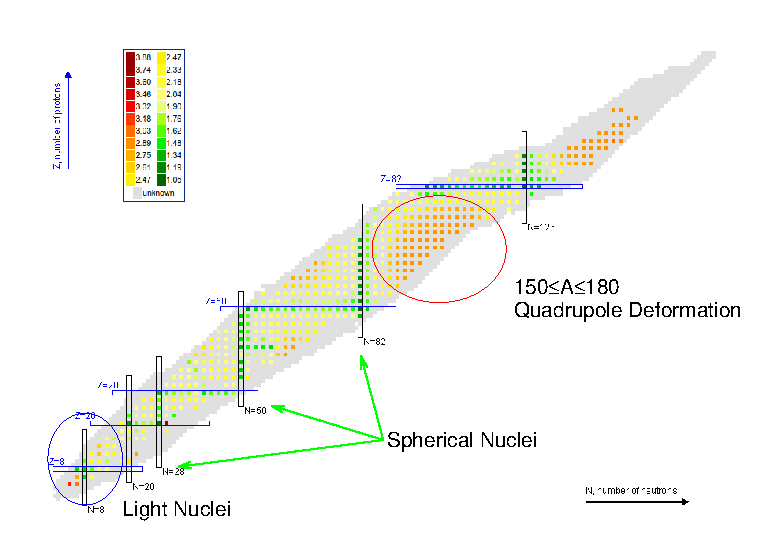
\includegraphics[width=\textwidth]{Chart_of_Nuclides_def.eps}
\caption{Chart of nuclides showing the varying degrees of deformation (R$_\frac{4}{2}$ values for even-even nuclei). Orange colored squares mark a well-deformed ground state, with green representing spherical nuclei.}
\label{fig:chart_nuclides}
\end{center}
\end{figure}
% \newpage

The first of such phenomenon is the existence of small surface oscillations of spherical nuclei, in which the nucleus can exhibit a macroscopic, collective motion of nucleons about the spherical equilibrium shape. These vibrations about the spherical shape are well-documented and studied throughout the spherical mass ranges of the Chart of Nuclides as an excellent example of collective degrees of freedom in the nucleus \cite{Casten_text,Aprahamian_118Cd}. These vibrational quanta, or phonons, also manifest in higher-order excitations (a two-phonon vibration, a three-phonon vibration, etc) as superimposed vibrations built on top of other vibrations.

Vibrations, however, are not the only collective degree of freedom afforded to the nucleons in the nucleus; collective rotations of nucleons about an axis are abundant in nuclei \cite{Casten_text,Wong_text}. For spherical nuclei, a nuclear rotation is energy degenerate, as there is no change in the fundamental frequency of oscillation, but in deformed nuclei, we find strong experimental evidence of collective rotations about the different axes. Whenever a quadrupole deformed nucleus rotates about an axis, it will emit electric quadrupole radiation (E2 type radiation) \cite{Rowe_Wood_text}. We subsequently observe this strong rotational motion in the transition probabilities between nuclear states (B(E2) measurements quantized with a single-particle estimate) in Figure \ref{fig:nucl_rotation}, where the entire region of deformation exhibits strong ($>$50~Weisskopf unit strength) transitions, a very strong indication of collective motion.

An open question then arises: are there superimposed vibrations on top of a deformed ground state, much like the vibrations about a spherical shape?

\begin{figure}[h!]
\centering
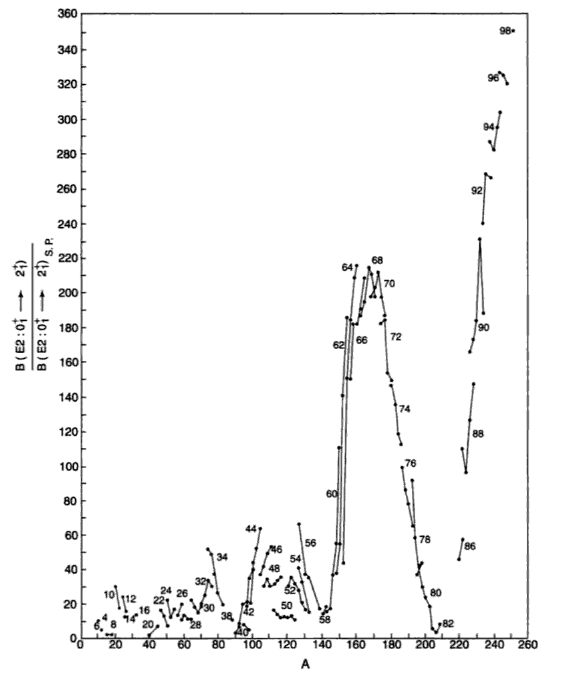
\includegraphics[width=0.95\textwidth]{B(E2)_rotations_Casten.png}
\caption{Measured B(E2) transition probabilities in single-particle units as a function of A, highlighting the region of deformation (as well as heavier actinide region) where strong nuclear rotations exist \cite{Casten_text}. \label{fig:nucl_rotation}}
\end{figure}
\newpage



% From this qualitative picture, we can observe several nuclear structure phenomena at a glance. Immediately, we see the \textit{magic} nuclei, incredibly well-bound and stable nuclei where Z or N are equal to 2, 8, 20, 28, 50, 82, or 126. This is an effect of the nuclear shell model (an analogue to the atomic electron shell model), where nuclei will fill sequential, discrete shells with nucleons, which can be used to determine properties of the nucleus by examining which shells are filled (or unfilled) with either protons or neutrons. We can represent the structure of the very light nuclei (fewer than $\sim$20 nucleons), as well as the nuclei near shell closures, with models like the nuclear shell model. However, the shell model begins to lose its applicability and interpretability as we add larger numbers of nucleons to the system, and as the nuclear ground state becomes less spherical.

\section{Deformation in Nuclei}\label{sec:nuclear_deformation}
% Spherical nuclei behave quite predictably under the shell model, yet as we stray farther away from the closed shells at the magic numbers and into the realm of deformed nuclei, this model begins to break down and becomes extremely (if not impossibly) complicated and computationally intensive. For perspective, ``To quote the famous example of Talmi, in $^{154}_{62}$Sm$_{92}$, approximately 3$\times$10$^{14}$ [J$^\pi$=]2$^+$ states can be constructed with" its combination of protons and neutrons via shell model considerations \cite{Casten_text}. The gravity behind this statement should not be understated, as the Samarium-154 nucleus contains a \textit{modest} number of nucleons, even in comparison to the similarly deformed nucleus, yet significantly more massive, $^{184}_{74}$W$_{110}$. If we are to realistically model the structure of nuclei (most of which are \textit{not} spherical, especially above A$\approx$20), more exotic methods must be implemented by expanding the microscopic nature of particle-hole excitations in the nucleus. This is done by introducing pairing correlations into the nuclear wavefunctions, in a departure from the single-particle nature of the shell model. 

%rotational nuclei, deformed ground state

Description of collective motion for a deformed nucleus begins by treating the nuclear radius as a liquid drop with the statically deformed shape shown in Equation \ref{eq:def_radius}, and then allowing the deformation parameters to deviate in small amplitudes. The work contained in this dissertation is strictly concerned with static, prolately deformed nuclei, or where $\gamma$=0 and $\beta>$0, although other nuclear shapes exist for negative values of $\beta$ (oblate, axially asymmetric, etc). This deformed nuclear shape is equivalent to a permanent quadrupole deformation in the ground state, or where $\lambda$=2 from Equation \ref{eq:def_radius}. It is also convenient and prudent to recast the angular momentum of states in the deformed nucleus as a projection of the total angular momentum along the axis of symmetry (K$^\pi$); this is beneficial, as it helps us easily identify and distinguish the different types of collective motion in deformed nuclei. K$^\pi$ can further be distinguished by the parity of states, as is typical by a $\pi$=(-1)$^\lambda$ rule, where this is also a clue to the asymmetry of nuclear wave functions.


Effects due to the pairing of nucleons in discrete shells and subshells in the nucleus have a profound effect on the structure of states in the deformed nucleus. In one of the most important pairing effects, the pairing of fermions in discrete shells forbids particles from occupying the same space, so when two protons or neutrons pair together to create an excitation (or as the even-even nucleus resides in the ground state). However, there is an energy intrinsic to the nucleus at which two nucleons will break their tendency to couple together as pairs; this pairing gap for protons and neutrons (2$\Delta_{\pi}$ \& 2$\Delta_{\nu}$ respectively) is taken from \cite{MANG_pairing1965353}, and is a measure of the odd-even staggering of energies caused by the pairing interaction in the nuclear binding energy. In the rare-earth region of nuclei, this pairing gap is experimentally observed near $\sim$1.5-2.0~MeV, where the states below this energy are the signatures of macroscopic collective motion of nucleons (or in terms of pairing, multiple quasiparticle pairs acting in the form of vibrational phonons) as a whole, in a dramatic shift away from independent/single particle excitations \cite{Bohr_pairing1958}. These pairing effects then bring rise to the idea of nuclear excitations being created via quasiparticle pairs; this is stated in stark contrast to the rigid rules of the shell model where fermions (in the case of particle-hole states) will have defined occupancy of shells, and instead can exhibit partial occupancies. Above the pairing gap, we notice a sharp increase in level density, where we have state-mixing occurring between the particle, quasiparticle pair, and collective configurations, and as such, finding a `pure' collective vibration becomes increasingly difficult \cite{Casten_text,Heyde_text}.


% The energies of quasiparticle excitations simplifies the picture of the shell model immensely, in that these energies are expressed relative to the absolute Fermi energy, which condenses the entire occupancy of the shell model down to a few excitations relative to this Fermi surface \cite{Casten_text}. 
% Since the quasiparticle energies are constructed with respect to the pairing gap 2$\Delta$, we can see experimental evidence of this pairing gap, which affects the level density, the sphericity of surface shape, and the microscopic character of states \cite{Casten_text}. With this key dinstinction between collective and single particle interactions in mind, the collectivity of states, not only below the pairing gap, but across the entire continuum of nuclear states is of paramount importance.  %The role pairing has on the nuclear excitation is that coherent pairs of nucleons cannot be formed above this gap, meaning the states above the gap \textit{cannot} be attributed to pair correlations. Any states below the pairing gap are surmised to be macroscopic collective vibrations. Data in the literature points to very few two-particle excitations below the pairing gap of any particular nucleus. 

The pairing gap for a particular nuclei $^A_Z$X$_N$ can be calculated with Equations \ref{eq:pairing_gapP} and \ref{eq:pairing_gapN}, where E(N,Z) is the binding energy of the nucleus X for the particular neutron number N and proton number Z combination, and E(N,Z+1) is the binding energy of a nucleus that has an added proton, E(N,Z+3) is the nuclear binding energy of the nucleus with three added protons, and so on. For example, the proton pairing gap for $^{162}$Dy would involve the binding energies of $^{162}$Dy, $^{163}$Ho, $^{165}$Tm, $^{161}$Tb, and $^{159}$Eu, for the respective entries in Equation \ref{eq:pairing_gapP}.

\begin{align}
2\Delta_{\pi}=\frac{1}{8}[16E(N,Z)+9E(N,Z+1)+E(N,Z+3)+9E(N,Z-1)+E(N,Z-3)] \label{eq:pairing_gapP}\\
2\Delta_{\nu}=\frac{1}{8}[16E(N,Z)+9E(N+1,Z)+E(N+3,Z)+9E(N-1,Z)+E(N-3,Z)] \label{eq:pairing_gapN}
\end{align}

\subsection{Vibrations in Deformed Nuclei}
Given some excitation energy, the deformed nucleus' excitations are not necessarily treated as single particle excitations, but instead as a movement of multiple nucleons \textit{collectively} (as a whole) throughout the nuclear shape as it rotates. In the mid-20$^{th}$ Century, theoretical treatments to describe a deformed nucleus emerged as the geometric collective model of Bohr and Mottelson \cite{BohrMott_text}, and one of the beauties of of this descriptive model was the near-immediate appearance of low-lying surface oscillations (in this case, nuclear vibrations) about the deformed ground shape \cite{BohrMott_text}, as well as the prevalence of fundamental nuclear rotations. These two modes of collective motion, vibration and rotation, make up the basic degrees of freedom available to a deformed nucleus, where, in stark contrast to the degenerate vibrations of a spherical nucleus, a vibration in a deformed nucleus can be along any of the axes of symmetry according to a time-dependent multipole expansion of the deformed shape. In its lowest order ($\lambda$=2 expansion of Equation \ref{eq:def_radius}), the nucleus \textit{can} exhibit quadrupole oscillations around its equilibrium shape in one of two possible types, a $\gamma$-vibration or a $\beta$-vibration. The notation and phenomenology behind these modes of vibrations alludes to the `direction' of oscillation with respect to the Hill-Wheeler coordinate parameterization mentioned earlier in \S\ref{sec:Nuclei_quantum_system}. For example, the $\gamma$-vibration is a dynamic oscillation that breaks axial symmetry (the parameter $\gamma$) to maintain a K$^\pi$=2$^+$ projection of angular momentum, while the $\beta$-vibration maintains both axial symmetry, as well as a K$^\pi$=0$^+$ projection of angular momentum (an oscillation of quadrupole deformation $\beta$). Note the positive parity, which indicates a reflection symmetry for the nuclear shape and corresponding wave functions. Crude cartoon visualizations of these quadrupole vibrations can be seen in Figures \ref{fig:beta_vibration} and \ref{fig:gamma_vibration}. In these pictures, the schematic on the left looks down the axis of symmetry (represented by bold, black lines), with the side view on the right. Thin black lines outline the deformed equilibrium shape, with dashed red lines showing the extent of the dynamic, quadrupole oscillations; blue arrows are meant to guide the eye as to how the nucleus changes shape. 

\begin{figure}[h!] 
\begin{center}
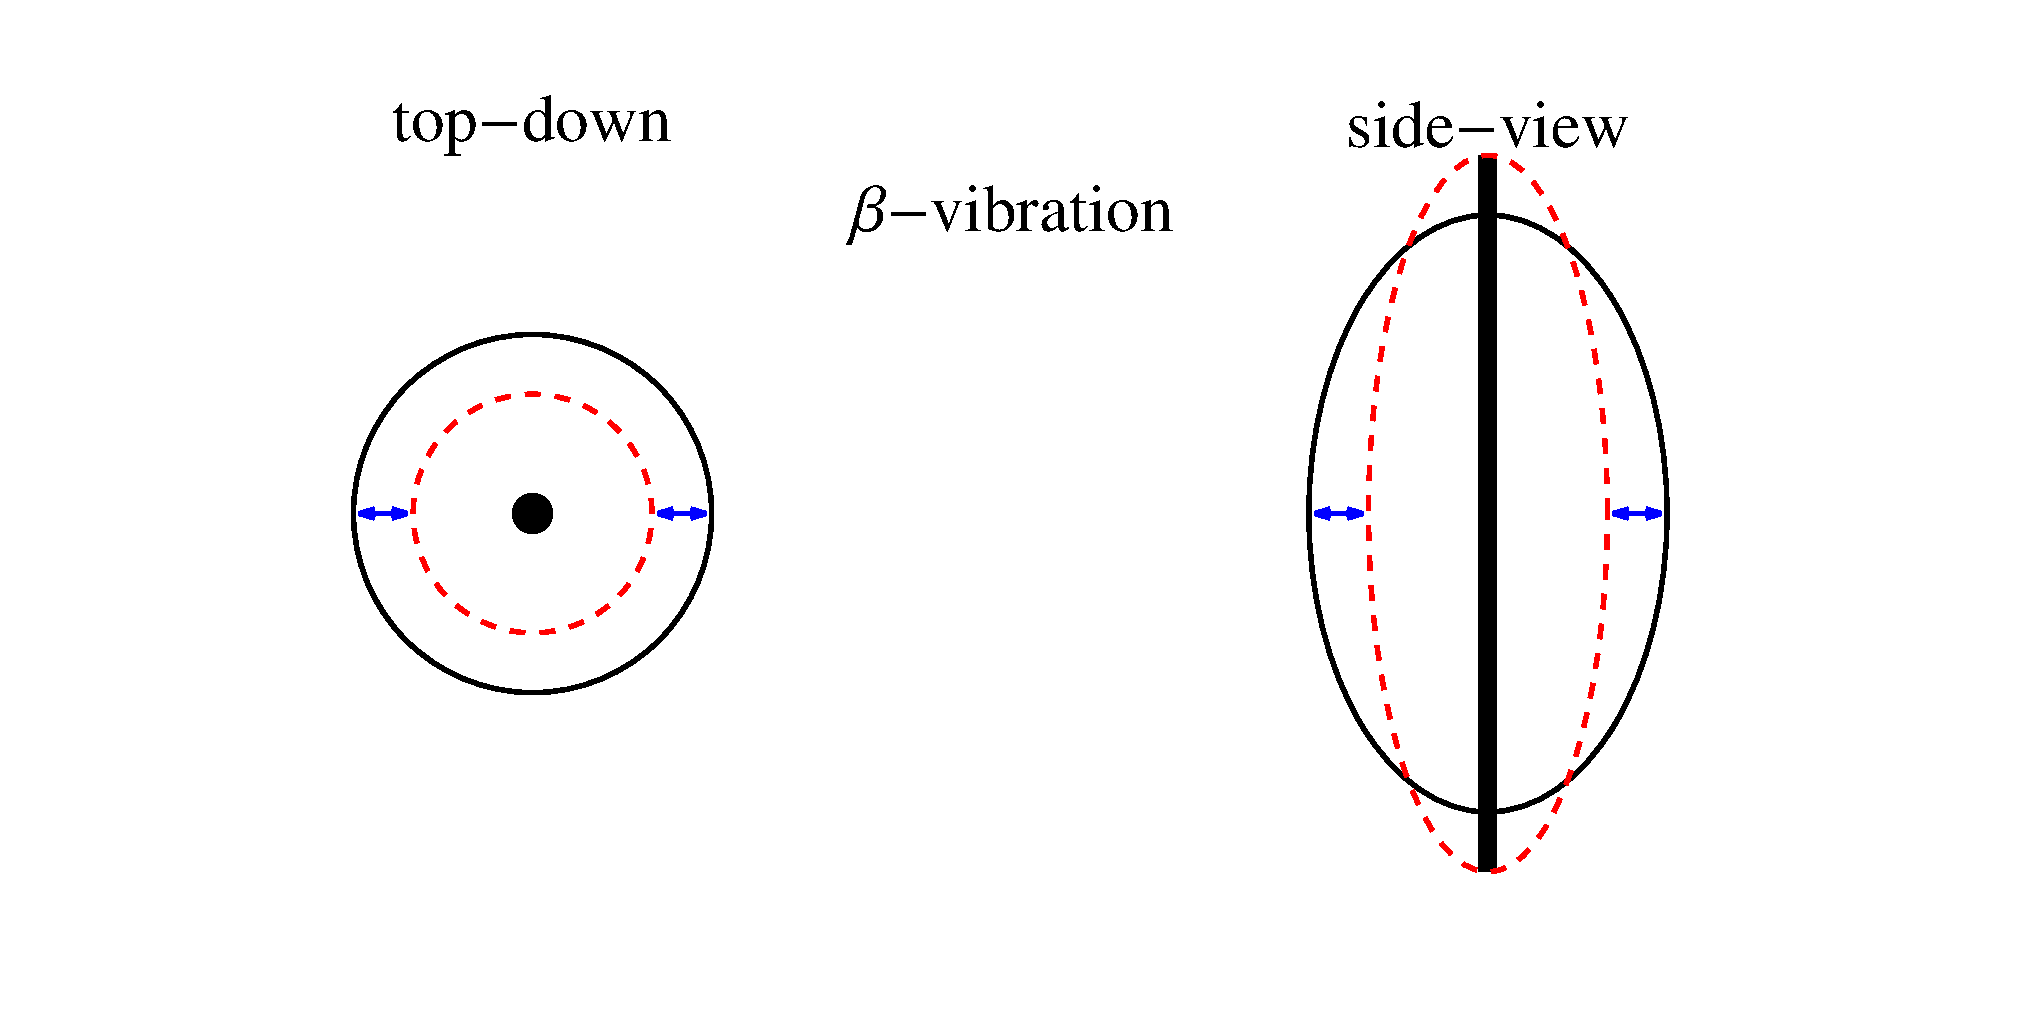
\includegraphics[width=\textwidth]{SciDraw_beta_vibration.eps}
\caption{Schematic of the $\beta$ quadrupole vibration about a deformed equilibrium shape.}
\label{fig:beta_vibration}
\end{center}
\end{figure}

\begin{figure}[h!] 
\begin{center}
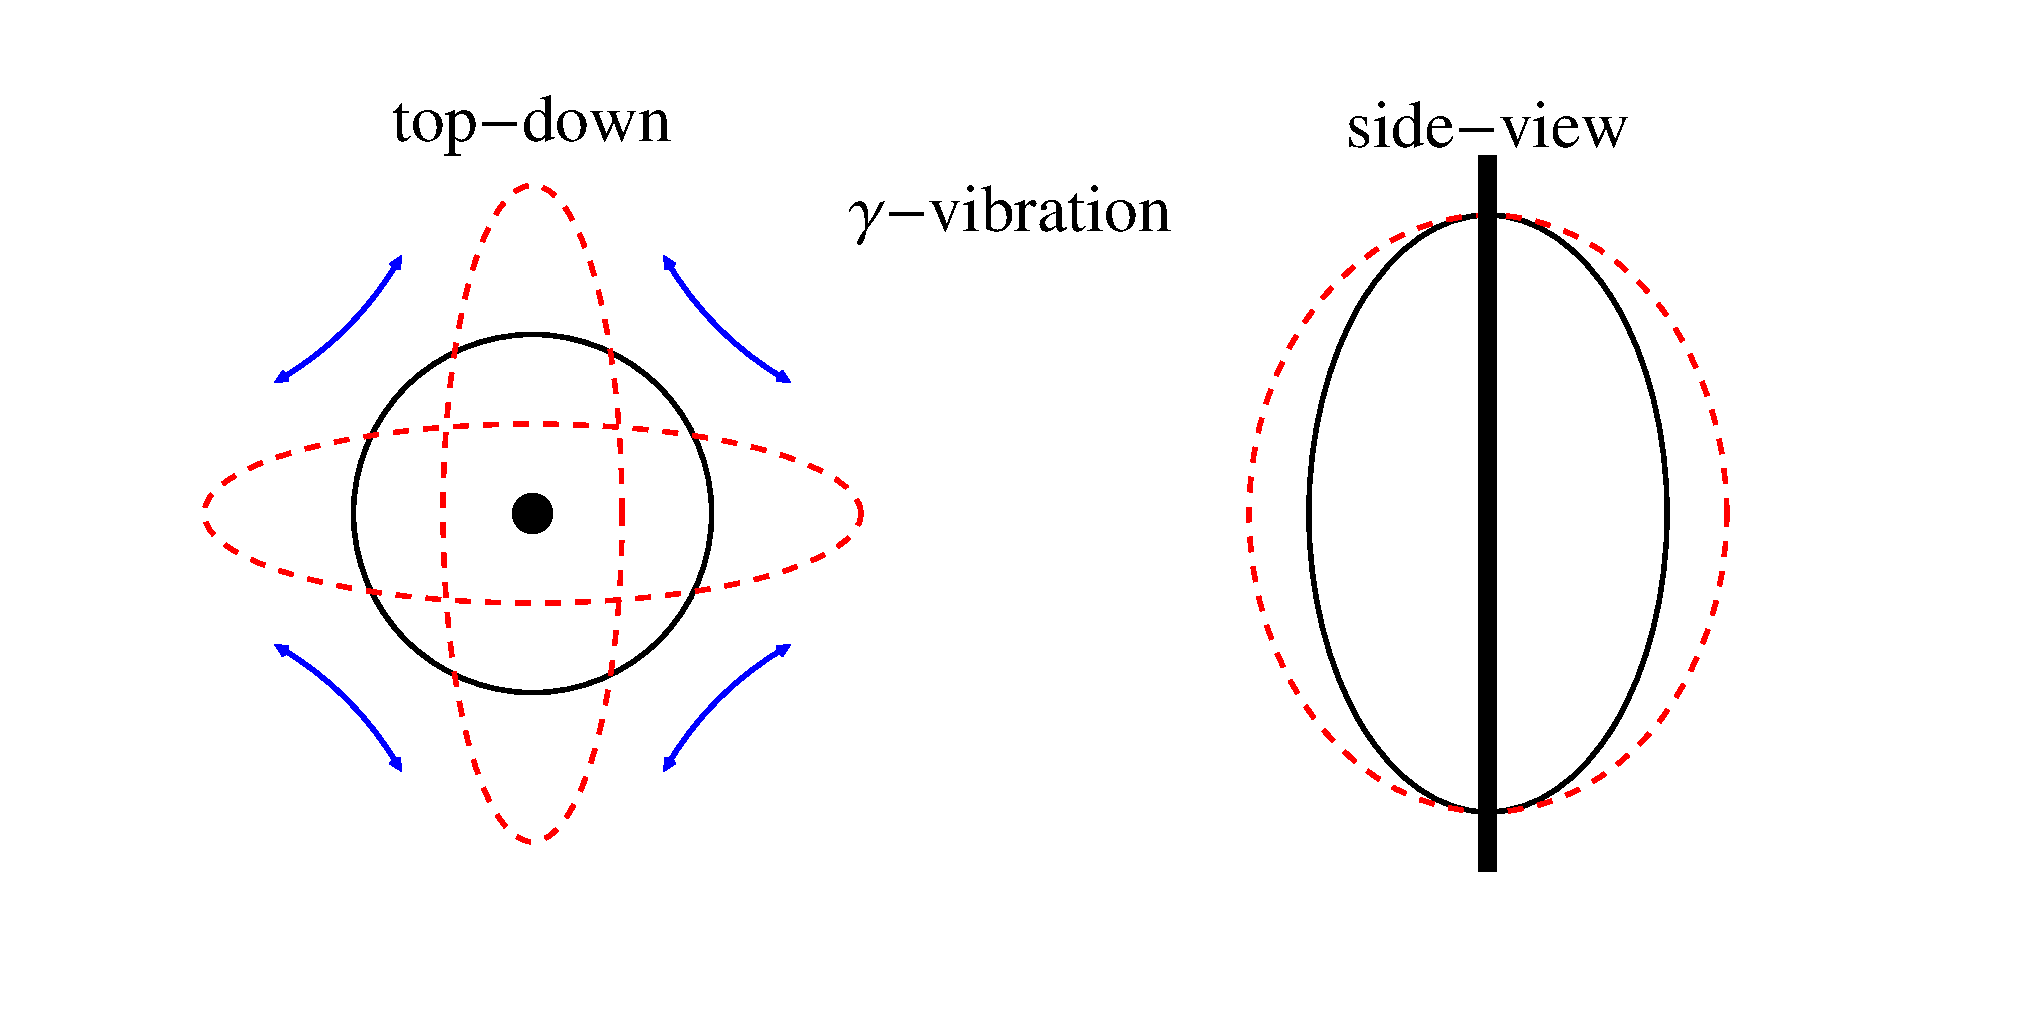
\includegraphics[width=\textwidth]{SciDraw_gamma_vibration.eps}
\caption{Schematic of the $\gamma$ quadrupole vibration about a deformed equilibrium shape.}
\label{fig:gamma_vibration}
\end{center}
\end{figure}

If a single vibrational phonon can be superimposed on the collective rotational ground state, how feasable is the two-phonon case for deformed nuclei? Linear combinations of the quadrupole phonon structure would involve the $\gamma\gamma$ (with either a 0$^+$ or 4$^+$ K$^\pi$ projection), $\beta\gamma$ (K$^\pi$=2$^+$), \& $\beta\beta$ vibrations (again, K$^\pi$=0$^+$). As an analogue to the classical harmonic oscillator problem, the addition of multiple phonon quanta will increase the energy of the system by some proportional amount, so we would expect a 2 phonon vibration to be double the energy of the 1 phonon vibration, or that E$_{phonon}\propto$N$_{phonon}$. \textit{In theory}, all modes of vibration should be obvious and abundant, but we will see that this is not immediately the case for deformed rare-earth nuclei given the current state of experimental data, especially with varying degrees of anharmonicity at play.

A further study in deformed nuclei is on the higher order octupole ($\lambda$=3 expansions of Equation \ref{eq:def_radius}) vibrations and if they can also exist, but the motions of the nuclear surface are significantly more difficult to envision as a drawing, especially on a 2-dimensional piece of paper. However, qualitatively, the octupole vibration is an asymmetric vibration about the quadrupole deformed nucleus in a `pear'-like oscillation. The octupole vibration (in spherical nuclei) manifests as a K$^\pi$=3$^-$ projection on the axis of symmetry, with asymmetric wave functions (and shape) due to the negative parity. However, in contrast to the degenerate quadrupole modes of K=0,2 in deformed nuclei, we expect a split-degeneracy of this K$^\pi$=3$^-$ projection into a quartet of possible projections, K$^\pi$=0$^-$, 1$^-$, 2$^-$, and 3$^-$ \cite{BohrMott_text} in the deformed nucleus.

%[PHONON EXPLANATION SOMEWHERE!!!!]
%really need to lay out some base for the phonon structure, energetics, etc
% The collective model is a purely geometric model of the behavior of nuclei, but is only broadly applicable in a moderate range of deformed nuclei. Alternative theories exist in an attempt to formulate a unified theory of structure that spans the bulk of the Chart of Nuclides, even in contrast to the somewhat limited scope of the shell model and geometric collective model. Beyond this traditional Bohr and Mottelson formalism, evolution of nuclear structure studies erupted in the early 1970s with Lie Algebraical based formulations.
%, even in contrast to the shell-model and geometric collective model.

% Iachello and Arima devised the Interacting Boson Approximation (IBA) to exploit the power of algebraic groups to model quantum systems, like the atomic nucleus. Exact symmetries from the set of algebraic groups can describe nuclear structure phenomena such as excitation energies, reduced transition probabilities, and branching ratios, very quickly and and with widespread success. An elegant treatment, the IBA models the nucleus' valence nucleons as aggregate pairs of \textit{s} and \textit{d} bosons, with L=0 and L=2, respectively; the set of all substates of boson, the single monopole and five non-degenerate quadrupole bosons (\textit{s}, \textit{d$_{-2}$}, \textit{d$_{-1}$}, \textit{d$_{0}$}, \textit{d$_{1}$}, and \textit{d$_{2}$}) span a 6-dimensional space, represented by the unitary Lie Algebra group U(6). The decomposition of the U(6) group into the triplet subgroups of U(5), SU(3), \& O(6) lays down the framework to describe fundamental properties of nuclei. Each subgroup describes a separate `category' of nuclei, with textbook examples of nuclei that exhibit analogues to the expected geometrical behavior, with U(5) representing a purely harmonic vibrator, O(6) providing symmetries to describe an axially asymmetric `$\gamma$-soft' nucleus, and SU(3) gives rise to the deformed rotor. Each of these symmetries gives rise to irreduceable representations within the IBA, from which, we can make statements about the structure of states in the nucleus.
%Each subgroup contains distinct properties about the nucleus, including expected energies of excited states, transition probabilities between states, as well as selection rules for decays 
% The IBA is not without its limitations, the basis states set up by each subgroup cannot perfectly reproduce the specific nuclear structure of most nuclei, but at the very least, it provides a baseline understanding of structure.

% By forming the nuclear Hamiltonian ($\mathcal{H}\Psi=E\Psi$) in terms of the s or d boson creation and annihilation operators ($s^\dagger$, $\tilde{s}$, $d^\dagger$, $\tilde{d}$), we can write the standard IBA Hamiltonian as Equations \ref{eq:IBA_H} and \ref{eq:IBA_Q}. The structure that arises from one of the three subgroups is referred to as a \textit{dynamical symmetry} \cite{Casten_text}, where each symmetry contains distinct properties about the nucleus, including expected energies of excited states, transition probabilities between states, as well as selection rules for decays. For example, the extreme limiting case of the SU(3) symmetry states that the lowest K=0,2 bands stem from the same irreduceable representation, and as such, strong transitions from these states cannot be connected to the ground state band \cite{Casten_text}. We will find that in many cases, using the strict limits of each symmetry offers very little room for flexibility in a realistic, nuclear system. So from here, we can easily represent nuclei belonging to the three dynamical symmetries by this three parameter space, $\varepsilon$, $\kappa$, and $\chi$. Calculations for any nucleus can now be done by varying one or more of these parameters, with extreme ease, and without adding needless complexity to the system.
% \begin{align}
% \mathcal{H}(\varepsilon,\chi,\kappa)=\varepsilon n_d+\kappa\mathcal{Q}\cdot\mathcal{Q}\label{eq:IBA_H}\\
% \mathcal{Q}=s^\dagger\tilde{d}+d^\dagger\tilde{s}+\chi[d^\dagger\tilde{d}]^2\label{eq:IBA_Q}
% %\frac{\varepsilon}{\kappa}=4N\frac{1-\zeta}{\zeta}\label{eq:IBA_param}
% \end{align}

% A useful way to visualize the parameter space that describes U(5), SU(3), and O(6) nuclei is best seen in the IBA Symmetry Triangle, seen in Figure \ref{fig:Casten_Triangle}. This Symmetry Triangle maps out the parameter space of $\varepsilon$, $\kappa$, and $\chi$ that correspond to the limits of the different U(6) symmetries. However, this implies that nuclei do not have to ascribe to the very rigid limits of any particular symmetry (this is generally the case for most nuclei); `transitional' approaches must be made, where the open parameters for each symmetry become intermediate values along the `legs' or `arcs' in the IBA symmetry triangle (Figure \ref{fig:Casten_Triangle}). 
% 
% Physical phenomena are kept close at hand with the IBA with this low-parameter model; on a general scale with the IBA Hamiltonian (Equation \ref{eq:IBA_H}), we can attribute the first term, $\varepsilon n_d$, to the a spherical shape and structure, with any physics that determines deformation governed by the $\kappa\mathcal{Q}\cdot\mathcal{Q}$ term. One of the fundamental aspects of nuclear structure inside the IBA Hamiltonian (and throughout most models) is the importance of E2 transitions, in this case, simply related to $\mathcal{Q}$ by Equation \ref{eq:IBA_E2}, where e$_B$ is an effective boson charge \cite{Casten_text}.
% \begin{equation}\label{eq:IBA_E2}
% \mathcal{T}(E2)=e_B\mathcal{Q}
% \end{equation}

% These simplistic approaches to describing nuclear structure phenomena are a common theme with the IBA, by keeping the physics represented by the algebraic symmetries very accessible, while also providing limiting cases of `ideal' behavior from any of the pure dynamical symmetries.
%cite a bunch of IBA papers in the field here

%SU(3) is too strict (Casten 278)
%[IBA 1969-1975]
%PUBLISHED IN 87

%SHOULD ONLY HAVE TO GO INTO DETAIL ABOUT SU(3)
% \begin{figure}[h!] 
% \begin{center}
% 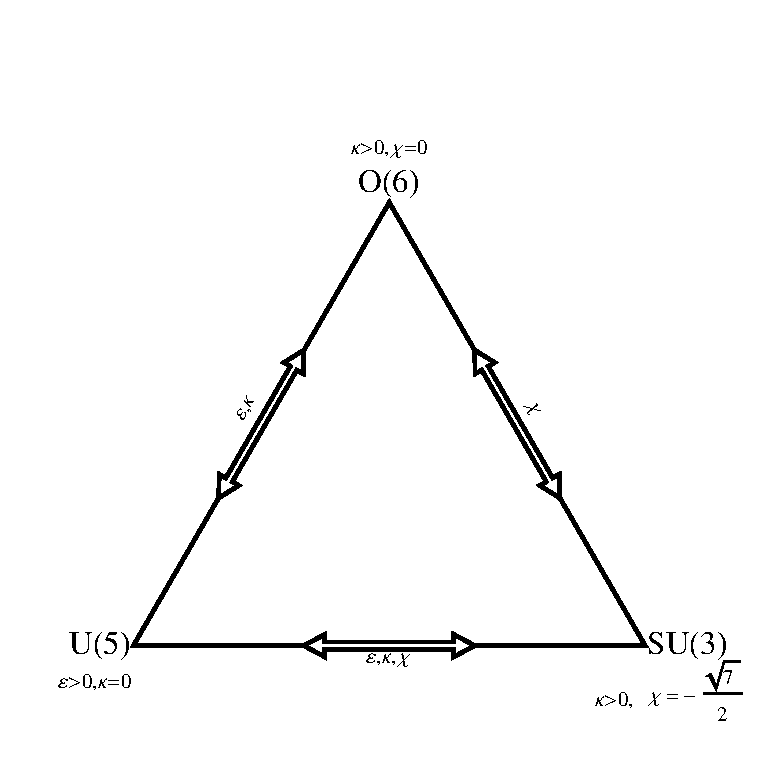
\includegraphics[width=\textwidth]{Casten_Triangle.eps}
% \caption{IBA triangle containing SU(3), U(5), \& O(6) symmetry limits with corresponding $\varepsilon$, $\kappa$, and $\chi$ parameters. Arrows on the `legs' of the triangle indicate which parameters are varied to perform a transitional nucleus' calculation.}
% \label{fig:Casten_Triangle}
% \end{center}
% \end{figure}

%IBA+F boson to take care of negative parity states (Barfield ref)
\section{Excited States in Deformed Nuclei}\label{sec:excitedstates}
The question then arises: what would these quadrupole and octupole vibrations look like represented as low-lying excited states in the level scheme of a well-deformed rotational nucleus? A cartoon level scheme representing the lowest lying quadrupole and octupole vibrations is given in Figure \ref{fig:phonon_def}, where we can immediately see the ensemble of states corresponding to each vibration, and each vertical `band' lines up with rotational members a particular vibrational state. Starting in the bottom left, we see the low-lying K$^\pi$=2$^+$ and 0$^+$ bands as the $\gamma$ and $\beta$-vibration (where one would expect near $\sim$1~MeV excitation energy). Then, continuing upward, the single-phonon vibrations of $\gamma$ and $\beta$ type have their corresponding two-phonon counterparts and combinations ($\beta\beta$, $\beta\gamma$, and $\gamma\gamma$) drawn at twice the excitation energy that assumes a completely harmonic vibration.

\begin{figure}[h!] 
\begin{center}
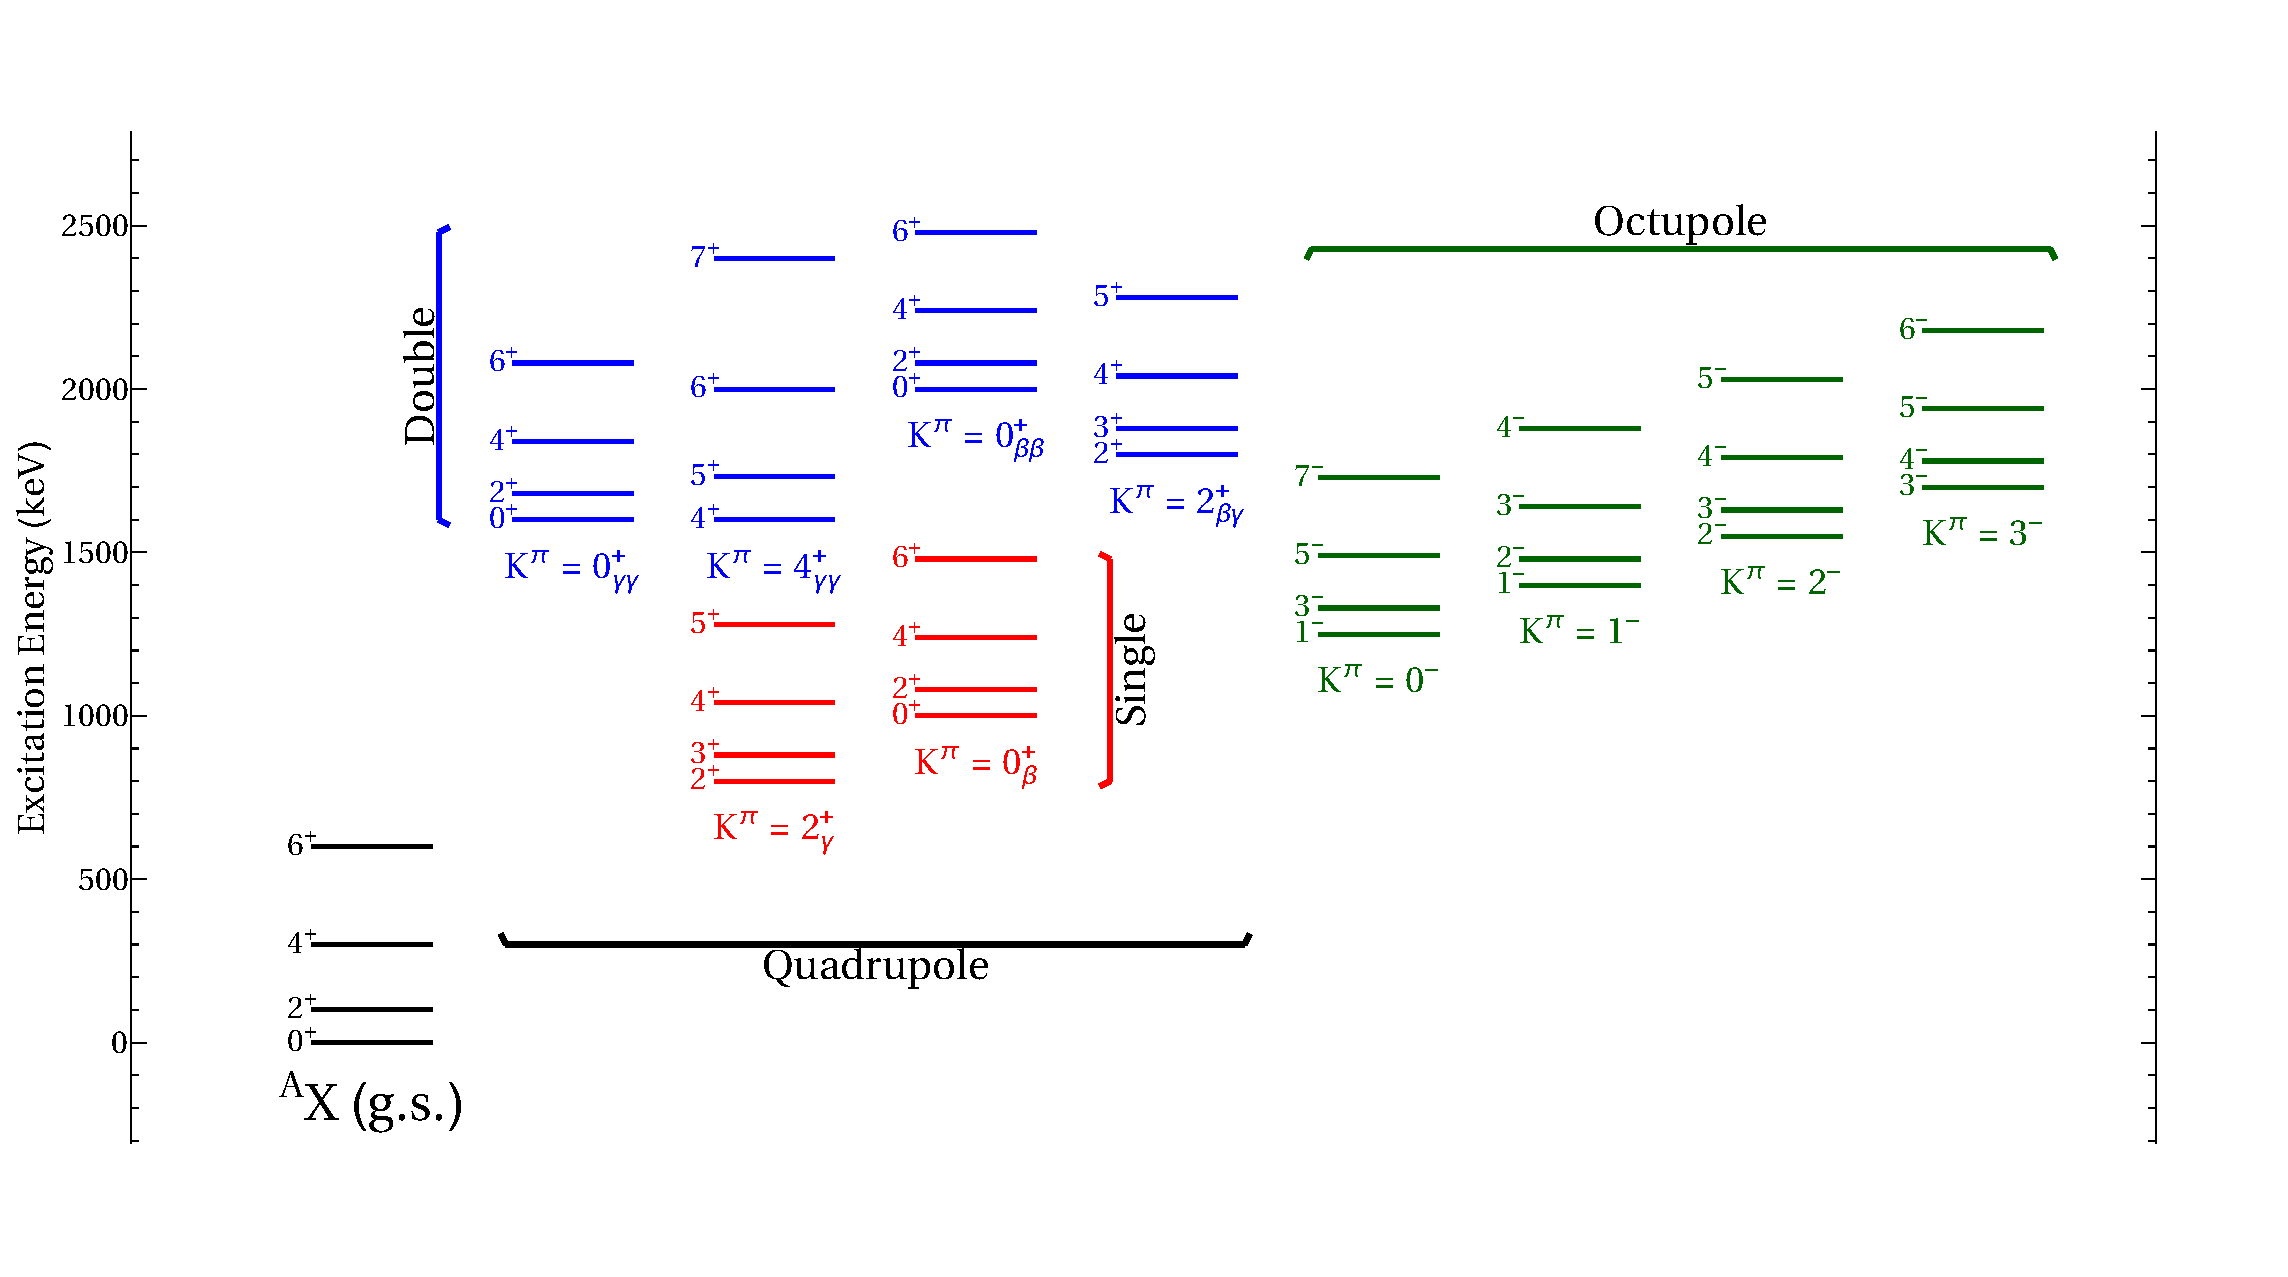
\includegraphics[width=\textwidth]{phonon_deformed.pdf}
\caption{Schematic level scheme of the single- and double-phonon vibrational (quadrupole and octupole) bands expected in deformed nuclei (color online).}
\label{fig:phonon_def}
\end{center}
\end{figure}

Nuclear rotations are superimposed on the base vibration expected for each type of phonon as band excitations, (single quadrupole/octupole and double quadrupole) according to the J(J+1) rule set out in Equation \ref{eq:rotation} for low values of K, of which would include the single- and double-phonon vibrational states (K=0,2,4). These additions of rotational energy directly correlate to higher-lying members of a band, with $\mathcal{I}$ being the moment of inertia for the nucleus. The rotational excitations in a band carry a set of spins related to the band's value of K; for K$\neq$0, J progresses through K,K+1,K+2... where only even spins occur in a K=0 band \cite{Greiner_Maruhn_text}.

\begin{equation}\label{eq:rotation}
E_{rot}=\frac{\hbar}{2\mathcal{I}}[J(J+1)] % for low values of K, at least
\end{equation}

% The lowest lying state of a particular band will (with the exception of a K$^\pi$=0$^-$ band) always have J$^\pi$=K$^\pi$ (\textit{e.g.} the bandhead of the K$^\pi$=0$^+$ band will be a J$^\pi$=0$^+$ excitation), where the spins and parities of other members (the superimposed rotations) of the band are selected by the selection rules outlined in Table \ref{tab:JK_selection}. In short, K$^\pi$=0$^\pm$ will contain \textit{every other} spin-parity, while any other projection of K simply counts up J$^\pi$ from the bandhead value. For example, a K$^\pi$=0$^+$ band will have J$^\pi$=0$^+$, 2$^+$, 4$^+$ (and so on) members, a K$^\pi$=0$^-$ band will contain similarly structured 1$^-$, 3$^-$, 5$^-$ (\textit{ad infinitum}) members, where a K$^\pi$=7$^+$ band has 7$^+$, 8$^+$, and so on.
% 
% \begin{table}[h!]
% \centering
% \begin{tabular}{r|c|c|c}
% & K$^\pi$=0$^+$ & K$^\pi$=0$^-$ & K$^\pi\neq$0$^\pm$ \\
% \hline
% \hline
% J$^\pi_0$= & K$^+$ & (K+1)$^-$ & K$^\pm$  \\ 
% \hline
% J$^\pi_1$= & (K+2)$^+$ & (K+3)$^-$ & (K+1)$^\pm$  \\ 
% \hline
% J$^\pi_2$= & (K+4)$^+$ & (K+5)$^-$ & (K+2)$^\pm$  \\ 
% \hline
% $\vdots$ & $\vdots$ & $\vdots$ & $\vdots$  \\ 
% \end{tabular}
% \caption{Selection rules used to determine J$^\pi$ values of rotational members of a specific K$^\pi$ band. \label{tab:JK_selection}} %    
% \end{table}

In Figure \ref{fig:phonon_def}, we immediately see a key (and long-lived) question in nuclear structure physics: What are the nature of 0$^+$ excitations? From this ideal, toy picture, we already see three possible ways to make a K$^\pi$=0$^+$ excitation. Understanding the nature of these common, low-lying excitations in nuclei has been a cornerstone of nuclear structure in the rare-earth region for decades. Experimentally, the searches for the nature of 0$^+$ have been cloudy from the evidence of double-phonon states across the entire rare-earth region such as the $\gamma\gamma$-type vibration in several nuclei (\cite{Garrett_twogammaEr_1997}, \cite{Lehmann_doublegamma168Er_1998}, \cite{Aprahamian2002}) that exhibit strongly collective, anti-aligned combinations of the $\gamma$-vibrational phonon.

%%%%%%%%%%
Experimentally, many deformed rare-earth nuclei exhibit a low-lying excited K$^\pi$=0$^+$ and K$^\pi$=2$^+$ band, and were assumed to be the $\beta$ and $\gamma$ vibration, respectively. In practice, however, this assumption of vibrational character has come under fire in recent years and tends to fall apart due to several factors. First, we do not have a complete, unambiguous characterization of each 0$^+$ state in the rare-earth region as a collective $\beta$-vibration; this stems from a lack of lifetime information (and thus transition probability information) of the K$^\pi$=0$^+$ bands in rare-earth nuclei.

\begin{figure}[h!]
\begin{center}
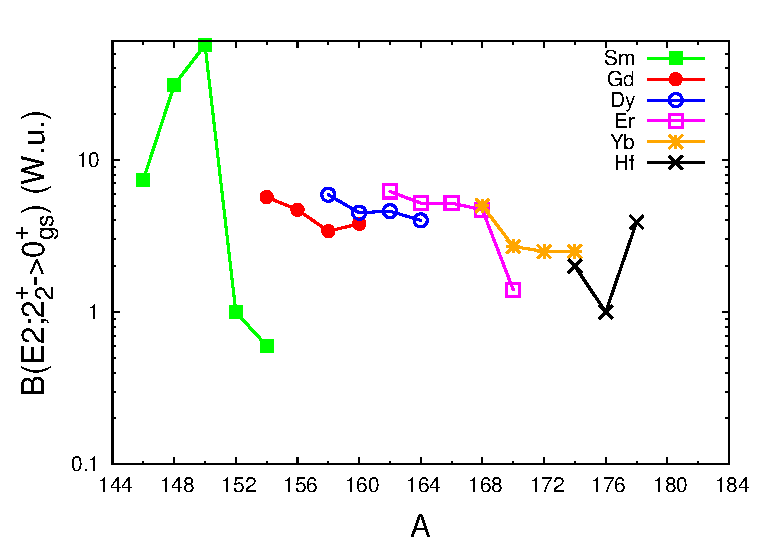
\includegraphics[width=0.88\textwidth]{Rare_Earth_2g_BE2.eps}\\
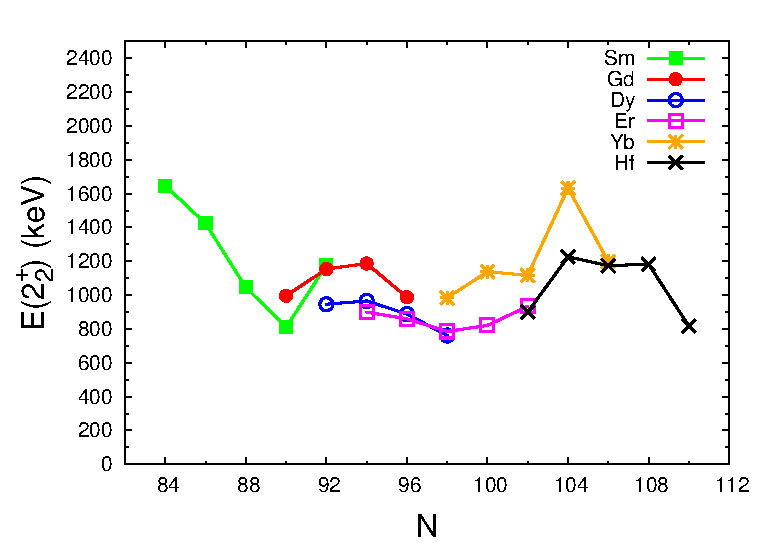
\includegraphics[width=0.88\textwidth]{Rare_Earth_2g_N.eps}
\end{center}
\caption{Absolute B(E2;2$^+_\gamma\rightarrow$0$^+_{gs}$) (in Weisskopf units) measurements for rare-earth nuclei, showing the uniformity of the $\gamma$-vibration in a deformed nucleus. The bottom plot shows the energy of the 2$^+$ bandheads as a function of N, highlighting the smoothly varying energies. \label{fig:Rare_Earth_2g_BE2}}
\end{figure}

Second, examination of the B(E2) transition probabilities and energies of the lowest-lying 0$^+$ and 2$^+$ bands yields a contrasted picture for each (assumed to be) vibrational type, shown in Figures \ref{fig:Rare_Earth_2g_BE2} and \ref{fig:Rare_Earth_02_BE2}. In the case of $\gamma$-vibrational characteristics, we observe a smoothly varying energies across the entire region, with the same behavior for the overall collectivity of these states (falling around 5~Weisskopf unit strength). However, the $\beta$-vibrational systematics become quickly obscured, with both obvious gaps in the lifetime information, an order of magnitude variance of the transition probabilties, and a less than smooth variance in energies like their $\gamma$-vibrational cousins! 



\begin{figure}[h!]
\begin{center}
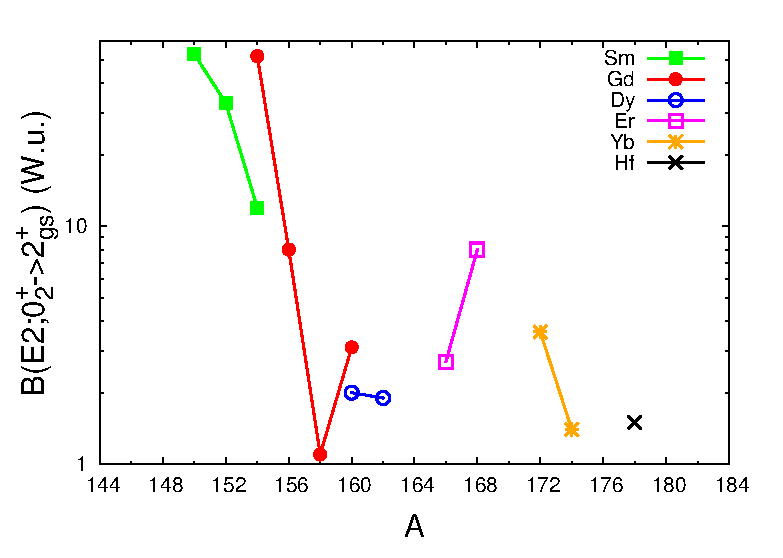
\includegraphics[width=0.88\textwidth]{Rare_Earth_02_BE2.eps}\\
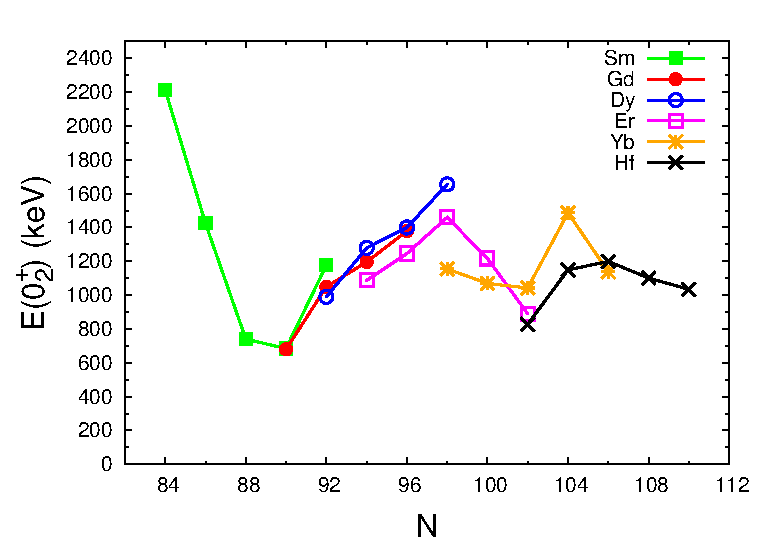
\includegraphics[width=0.88\textwidth]{Rare_Earth_0s_N.eps}\\
\end{center}
\caption{Absolute B(E2;0$^+_2\rightarrow$2$^+_{gs}$) (in Weisskopf units) measurements for rare-earth nuclei, showing the scattered experimental data that spans an order of magnitude variance. The bottom plot shows the energy of the 0$^+_2$ bandheads as a function of N, which shows a slightly more variant energy systematic than the 2$^+$ bandheads. \label{fig:Rare_Earth_02_BE2}}
\end{figure}

The emergence of the nuclear data that gives this unclear picture (particularly of the scattered B(E2) strengths) has garnered significant skepticism of \textit{any} vibrational degrees of freedom in the nucleus \cite{Garrett_betavib2001}. The story is \textit{still} unclear on the nature of any vibrational states in deformed nuclei due to the incomplete data surrounding it; if any clarification is to be made, we need lifetime information to say one way or the other.


By a similar merit for the octupole vibration, in Figure \ref{fig:phonon_def} we see the split quartet of low-lying negative parity states, as expected, yet these $\lambda$=3 excitations are not as well studied as their quadrupole counterparts \cite{Casten_text}. Several different phenomena occur in the low-lying negative parity states of deformed nuclei, including an inversion in the energy ordering of states as N increases, irregularities among the transition probabilities (as a function of $\Delta$K) throughout the rare-earth region of nuclei, among others \cite{Borner_collective1999,Casten_text}. Continue the multipole expansion to higher-order terms, and the hexadecapole ($\lambda$=4) vibrations appear. Again, we state here that these negative parity states and higher-order vibrational phonons have not seen the same order of experimental rigor and study as their $\lambda$=2 counterparts have; this work hopes to aid in the lack of vital lifetime information on low-lying negative parity states in the deformed region of nuclei. Systematic behavior of negative parity states (as well as the strength of quadrupole vibrations) varies wildly across the entire rare-earth region of nuclei and have been caught in the epicenter of experimental focus in nuclear structure in the past several decades. 

Much like the quadrupole counterparts, we can also picture a structure of coupled quadrupole-octupole-type phonons to either octupole or quadrupole phonons, further increasing the possible K-projections available to study \cite{Pascu_octupole_2015}. For example, a 2$^+\otimes$3$^-$ coupling can produce projections of 1$^-$, 2$^-$, 3$^-$, 4$^-$ \& 5$^-$, if we follow the same parity and triangle selection rules inherent to quantum systems. 

% In terms of the IBA, particular energetics and selection rules emerge from each dynamical symmetry that govern the overall behavior of the nuclear structure. For example, a pure SU(3) deformed rotator has specific ratios of reduced transition probabilities expected, as well as an expected grouping of K=0,2 excited bands inside of the same irreduceable representation \cite{Casten_text}. For example (and in stark contrast to the geometric model where they are discrete types of vibration), the K=0 band is interpreted as an excitation built on top of the K=2 $\gamma$-vibrational band, where we would expect to observe strong transitions between the bands, with weak transitions to the ground state band.
%outline some IBA symmetries and expected B(E2)'s or whatever
%The Pauli principle has a profound effect on the evolution of nuclear structure; energies of excited states and branching ratios are affected by the pairing of nucleons





  
\section{Historical Impetus in Experimental Nuclear Structure}\label{sec:study_of_0plus}
Experimentally, how have these low-lying excitations in deformed nuclei been studied in the past? The study of collective vibrational states has been a pressing issue in nuclear structure for decades, with the constant evolution of experimental techniques and theoretical models throughout the mid-to-late 20$^{th}$ Century \cite{Casten_text,PhysRevC.54.679,KORTEN_1993}. Categorization of 2$^+$ $\gamma$ vibrational bands across the region of deformation arose quickly, but their significantly more elusive cousins in the 0$^+$ states proved to be more difficult to ascertain an origin. A major contributor to their elusiveness stems from the difficulty experimentalists had in detection of these states in the first place; experimentation was simply not senstitive enough to capture signatures of the L=0 states! 

Near the turn of the millennium, however, in one of the pioneering (and one of the most-cited) works in the field, Lesher \textit{et.~al} found a surprising, completely unprecedented number of excited 0$^+$ states in deformed $^{158}$Gd \cite{Lesher_158Gdpt}. This work utilized the Q3D magnetic spectrograph at M\"{u}nich with two-nucleon transfer reactions, a particularly adept way to find J$^\pi$=0$^+$ excitations, where seven new 0$^+$ excitations (of thirteen total) were discovered. The Q3D was to later be used by D. Meyer in 2006 to continue this newly sparked renaissance of nuclear structure studies on the nature of 0$^+$ excitations in deformed nuclei \cite{Meyer_pt0_2006}, measuring 84 new 0$^+$ states. 

Recall from \cite{Rowe_Wood_text} the Pauli principle that governs nucleon pairing; first, the pairing of nucleons governs the J=0 ground state of even-even nuclei. Second, in a two nucleon transfer reaction, (p,t) or (t,p), the paired neutrons entering or exiting the nucleus will preferrentially couple to J$^\pi$=0$^+$ states. For an even-even nucleus with a 0$^+$ ground state, transfer reactions have a high overlap to this mode of excitation to J$^\pi$=0$^+$, giving the Q3D spectrograph its sensitivity. In the two nucleon transfer reactions angular distributions of outgoing tritons (or protons) are collected at various angles with respect to the beam direction by the opening of the spectrometer and bent through a series of 3 dipole magnets to a focal-plane detector (see Figure \ref{fig:Q3D}). Differing energies of ejectiles are bent by various amounts to the focal-plane detector, where positional dependence in the detector is directly related to the energy of the excited state populated ($E_x$), according to Equation \ref{eq:Q3D_E}. The remarkable resolution produced by the setup of quadrupole and dipole magnets propeled the Q3D above previously unattainable levels of discrimination, and has forever changed the field of nuclear structure.

\begin{equation}\label{eq:Q3D_E}
E_{ejectile}=E_{projectile}-Q-E_x-E_{C.O.M.}
\end{equation}

\begin{figure}[ht]
\begin{center}
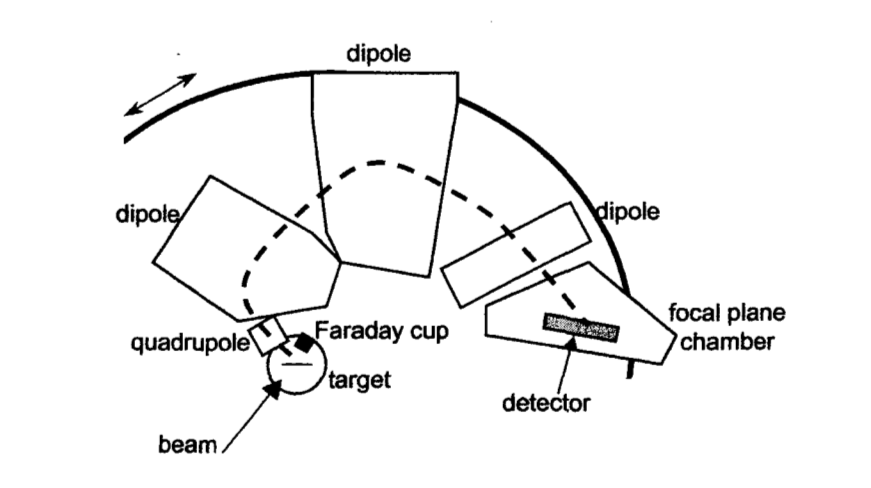
\includegraphics[width=\textwidth]{Q3D_spectrometer.png}
\caption{Schematic of the Q3D magnetic spectrograph at M\"{u}nich used for precision (p,t)/(t,p) spectroscopy \cite{Meyer_thesis}.}
\label{fig:Q3D}
\end{center}
\end{figure}


In the case of a $\Delta$L=0 transition, the angular distribution of detected particles will be extremely forward-peaked; this is an easily observed experimental signature, and is completely unique to $\Delta$L=0, as the measured intensity (differential cross section) can drop by an order of magnitude from $\sim$5$^\circ$ to $\sim$17$^\circ$ \cite{Meyer_pt0_2006}. Confirmation of the J$^\pi$=0$^+$ assignments can be made by comparing the relative cross sections from the experimental data to a Distorted Wave Born Approximation (DWBA) calculation, where an example of this can be seen in Figure \ref{fig:158Gdpt} for the 0$^+$ states in $^{158}$Gd.

\begin{figure}[ht]
\begin{center}
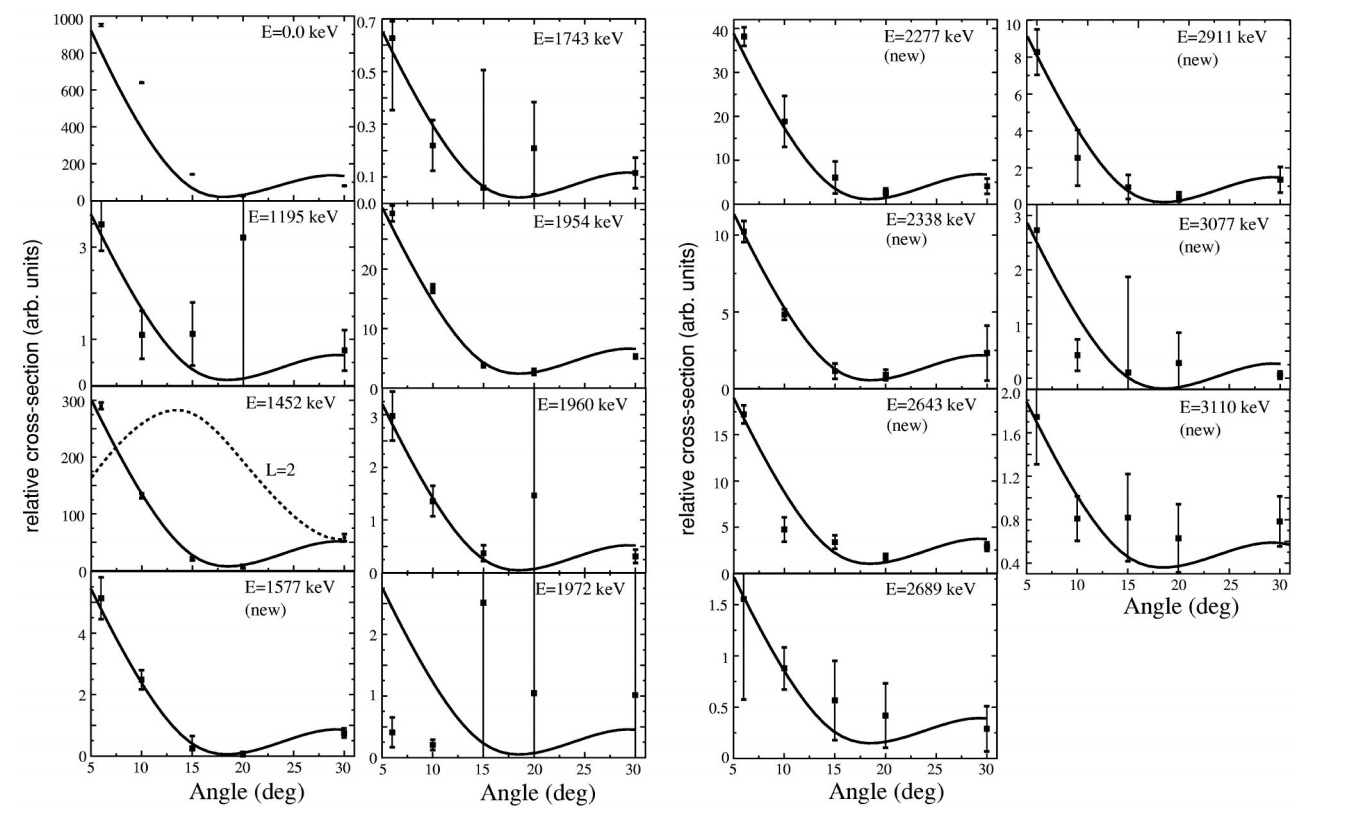
\includegraphics[width=\textwidth]{158Gd(pt).png}
\caption{Angular distribution data for all 0$^+$ states in $^{158}$Gd observed in the (p,t) reaction in \cite{Meyer_pt0_2006}. A DWBA calculation for an L=2 transition is shown as a dotted line in the E=1452~keV plot to show the unique nature of the L=0 transitions (in solid black).}
\label{fig:158Gdpt}
\end{center}
\end{figure}

This renaissance of (p,t)/(t,p) reaction studies has emerged in the past decade, as well as a coordinated flurry of theoretical and experimental efforts and campaigns to begin to answer the still open and important query of the nature of 0$^+$ excitations in the rare-earth region of nuclei \cite{WuAprahamian_multiphonon_1994, Aprahamian2004, Borner_collective1999, Garrett_betavib2001,RevModPhys.83.1467, Bonatsos_collective02009, Clark_pairtransfer2009, Pietrella_beta_2004, Zamfir_doubleoctupole_2002, Sun_0plusnature_PSM_2003}. Figure \ref{fig:Number_0s_Rare_Earth} shows the number of 0$^+$ states for rare earth nuclei, due in large part to the two nucleon transfer reaction studies by Meyer and Lesher \cite{Lesher_158Gdpt,Meyer_pt0_2006}.

\begin{figure}[ht]
\begin{center}
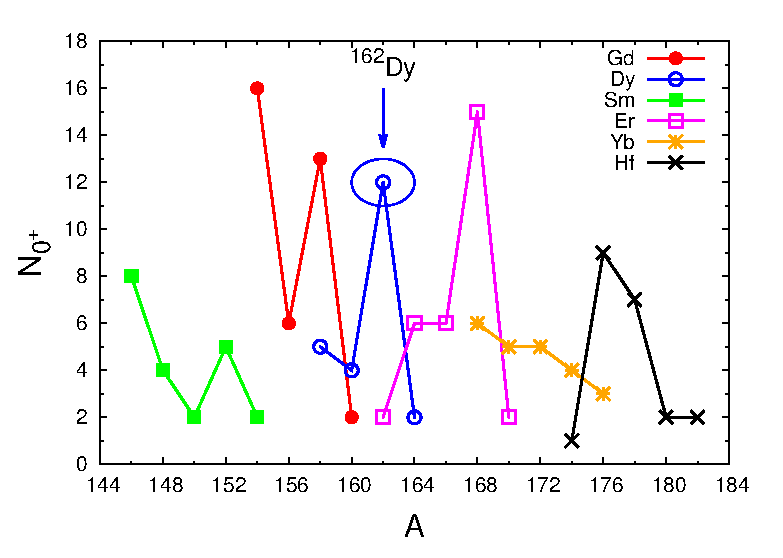
\includegraphics[width=0.95\textwidth]{Gd_Dy_0s_Number.eps}
\end{center}
\caption{Number of 0$^+$ states in rare earth isotopes of Sm, Gd, Dy, Er, Yb, and Hf. $^{162}$Dy is highlighted with a blue circle. \label{fig:Number_0s_Rare_Earth}}
\end{figure}
\newpage
%[MENTION THAT TRANSFER REACTION STRENGTHS TELL US A LITTLE ABOUT 0+ STATES]
In their recent review \cite{RevModPhys.83.1467}, Heyde \& Wood outline several criteria (key experimental fingerprints) to sucessfully elucidate the true nature of these 0$^+$ excitations. 
%, as well as significant proposals to improve the microsopic theories to describe the structure of nuclei far away from shell closures.

\begin{itemize}
\item[I.] Two nucleon transfer reaction strengths, (p,t) or (t,p)
\item[II.] Monopole E0 strengths, $\rho^2$(E0)
\item[III.] Absolute reduced transition probability measurements, B(E2;0$^+_i\rightarrow$2$^+_{g.s.}$)

\end{itemize}

Individually, the experimental quantities listed above cannot fully probe any collective nature of excitations within the nucleus, but in tandem, can uncover much of the mystery of the makeup of nuclear states.

In many cases (due in part to the pioneering (p,t) measurements made by \cite{Lesher_158Gdpt,Meyer_pt0_2006}) throughout the rare-earth region of nuclei, two nucleon transfer reaction strengths are available; the relative cross sections can provide a clue to pairing configurations in nucleons \cite{RevModPhys.83.1467}. This implies that a large relative cross section between two-nucleon transfers will signify a large single- or two-quasiparticle nature of a particular excited state. Historically, inflated two-nucleon transfer reaction cross sections between 0$^+$ states were observed as evidence of rapid shape change of the nucleus \cite{Clark_pairtransfer2009}. Multinucleon transfer reactions also offer a double-pronged attack, in that the spectroscopy can also find/confirm the existence of 0$^+$ excitations, recalling the (p,t) reactions outlined in \S \ref{sec:study_of_0plus}.

Monopole E0 transitions, the $\gamma$-ray forbidden decay of a 0$^+\rightarrow$0$^+$ transition, provide insight into a unique facet of the nuclear structure, as the transition is directly related to the mean-square nuclear radius, and thus, the extent of deformation. The measurement of E0 transitions offers clues to the nature of 0$^+$ states, but these experimental signatures are far from easy to obtain \cite{Heyde_text}. Since a $\gamma$-ray carries \textit{at least} one unit of angular momentum away from the nucleus, and no angular momentum transfer takes place in a 0$^+\rightarrow$0$^+$ transition, the nucleus must decay via internal conversion electrons. The transition probability of an E0 transition differs in form from the traditional $\gamma$-ray reduced transition probability (see \S \ref{sec:redtab}), but is expressed by the monopole strength, the internal conversion electron analogue, $\rho^2$(E0), instead. A similar amount of experimental and theoretical effort is being made in regards to the E0 transitions in rare-earth nuclei \cite{Ilie_E02011}. %Recent studies using the IBA have examined the behavior of E0 transitions in nuclei \cite{Ilie_E02011} at both the limits of the SU(3) symmetry and in the middle of the symmetry triangle, with connections to the collectivity of states discussed.

Finally, the absolute B(E2) transition probabilities (inversely proportional to the lifetime of excited states) are the largest clue to the collectivity of states, as they hold a vital part in testing both the IBA and the geometric collective model. The measurement of excited state lifetimes (as seen in the upcoming \S \ref{sec:why_lifetimes}) are the main focus on this work. 
%Garrett [REF HERE] (among many others) has shown that shape coexistence (similarities of nuclear shapes between states) is prevalent in excited states of $^{154}$Sm and $^{154}$Gd, nuclei close to the N=80 shell closure and not fully deformed shape, as well as the existence of double-phonon excitations in A~110 Cadmium isotopes [REF HERE]. 

Strong octupole shape correlations have been experimentally observed in spherical/transitional nuclei (and recently in neutron-rich $^{144}$Ba) by the observation of strong E3 multipolarity radiation that decays to the ground state \cite{Bucher_Octupole144Ba_2016,Garrett_2009_negShapeCoex}. Similarly, strong quadrupole-octupole coupling has been observed in the form of 2$^+\otimes$3$^-$ coupling in several cases by the observation of K$^\pi$=2$^-\rightarrow$2$^+_\gamma$ transitions \cite{Pascu_octupole_2015,Spiecker_E1strength,Soloviev_QuadHex}. In all of these cases, we see and stress the importance of reduced transition probabilities connecting nuclear states. One experimental observable that points toward any octupole correlation (as a means to measure reflection asymmetry, a signature of octupole deformation) is the measurement of E3-multipolarity radiation, which we do not employ in this work due to the lack of detection of this type of radiation. However, significant (albeit less than straightforward) emphasis is placed in the measurement of E1 radiation to study octupole vibrations in the deformed rare-earth region \cite{Pascu_octupole_2015,Soloviev_QuadHex}. 

%NEED TO TALK ABOUT HOW OCTUPOLE STATES HAVE BEEN STUDIED TOO
%REFERENCE THE DIFFERENT IBA WORKS DONE IN THE RARE-EARTH REGION

% \section{$\gamma$-ray Emission \& the Electromagnetic Interaction}
% For nuclear excitations well below the energy threshold for particle emission (a majority of excited states in nuclei), the preferred method to de-excite the nucleus is via the emission of a $\gamma$-ray. %This is extremely beneficial to the experimentalist in the laboratory, as modern detectors and instrumentation have evolved in such a way to make $\gamma$-ray spectroscopy a straightforward and common practice. 
\section{Assessing Nuclear Structure from Decay Radiation}
%Decay radiation in any form is the basis for nuclear structure phenomena, since any observed radiation must contain information about the configuration of the nucleus as it brings the nucleus from some initial state to a final state.
The detection of electromagnetic $\gamma$ radiation is of great value when studying the structure of the nucleus. Since $\gamma$-decay of the nucleus is one of the dominant methods of de-excitation for states below the energy threshold for particle emission, a link (some quantum mechanical operator) between two quantum states can be made via the electromagnetic Coulomb process. Usually expressed as a matrix element, Equation \ref{eq:matrix_element} is the manifestation of observables from some corresponding operator (in this case, the electromagnetic operator acting on the nuclear eigenfunctions). In the case of electromagnetic decays, the matrix elements of the E2 multipole transition operators remain a key facet of nuclear structure, as the quadrupole electromagnetic operator drives collective quadrupole transitions in nuclei, lending its importance almost immediately. Similarly, the other multipole expansions of the electromagnetic operator (isovector dipole, isoscalar dipole, octupole, etc.) directly link the charge distributions of two nuclear states, such as the E3 operator for octupole shape change.

\begin{equation}\label{eq:matrix_element}
\mathcal{M}_{fi}=\langle\psi_f\vert\mathcal{H}\vert\psi_i\rangle
\end{equation}

When studying excited states in nuclei, measurement of the transition probability (related to the matrix element) becomes the basis for understanding nuclear structure phenomena. 

% \subsection{Why Measure Lifetimes?}
\label{sec:why_lifetimes}
The transition probability ($\mathcal{W}$) for a $\gamma$-decay that de-excites the nucleus from an initial state to a final state can be expressed in terms of the mean lifetime ($\tau$), the average time the nucleus stays in an excited state, or by the half-life (\textit{t$_{1/2}$}). The exact relationship can be seen in Equation \ref{eq:life_halflife}.

\begin{equation}\label{eq:life_halflife}
\mathcal{W}=\frac{1}{\tau}=\frac{\ln2}{t_{1/2}}
\end{equation}

For an excited state with multiple $\gamma$-decay channels, we can expand the total $\mathcal{W}$ as a sum of all transition probabilities weighted by the branching ratio (BR$_i$) and internal conversion coefficient ($\alpha_i$) of each transition (Equation \ref{eq:BR_W}).

\begin{equation}\label{eq:BR_W}
\mathcal{W}=\sum_i\frac{BR_i}{\tau(1+\alpha_i)}
\end{equation}

The number of full mathematical derivations of Fermi's Golden Rule from time-dependent perturbation theory rivals that of Talmi's estimation of 2$^+$ configurations in Samarium-154 ($\sim$3$\times10^{14}$) \cite{Casten_text}. The exhaustive treatment can be seen in much greater detail in various sources (\cite{Wong_text},\cite{Heyde_text},\cite{BlattWeiss_text}), where (in this work) we will start with Fermi's Golden Rule \cite{Wong_text} in Equation \ref{eq:FermisGR}.

\begin{equation}\label{eq:FermisGR}
\mathcal{W}=\frac{2\pi}{\hbar}\vert\langle\psi_f\vert \mathcal{H}_{EM,int}\vert\psi_i\rangle\vert^2\rho(E_\gamma)
\end{equation}

Here, we can see the direct relationship between the nuclear matrix element and $\gamma$-ray energy-dependent density of states ($\rho$(E$_\gamma$)) to the transition probability, $\mathcal{W}$. This square of the matrix element describes the coupling of the nuclear-based interaction Hamiltonian to an external electromagnetic field, which brings the nucleus from some initial state $\vert\psi_i\rangle$ to a final state $\vert\psi_f\rangle$. This transition, for $\gamma$-decay in the nucleus, is represented by the electric or magnetic multipole operator(s) of order $\lambda$, $\mathcal{O}_{\lambda}$. From Wigner-Eckhart theory, we can remove any angular momentum dependence from the full matrix element ($\vert\mathcal{M}_{fi}\vert$=$\langle\psi_f\vert \mathcal{H}_{int}\vert\psi_i\rangle$) to give us the reduced transition probability in Equation \ref{eq:Wig_B}.

\begin{equation}\label{eq:Wig_B}
  B(\pi\lambda;J_i\rightarrow J_f)=\vert \mathcal{M}_{fi}\vert^2=\frac{1}{2J_i+1}\vert\langle J_f\vert\vert \mathcal{O}_{\lambda}\vert\vert J_i\rangle\vert^2
\end{equation}

Performing a multipole (and subsequent series) expansion of $\mathcal{O}_{\lambda}$ into the spherical Bessel functions, spherical harmonics, and the nuclear current density $\mathcal{J}$($\vec{r}$) (Equations \ref{eq:OE_operator} and \ref{eq:OM_operator}) \cite{Wong_text}, we arrive at Equation \ref{eq:W_B}.

%[explain matrix element as electromagnetic operator WONG182]
\begin{align}
  \mathcal{O}_{\lambda\mu}(E\lambda)=-\frac{(2\lambda+1)!!}{c(\lambda+1)k^{\lambda+1}}\mathcal{J}(\vec{r})\cdot\vec{\nabla}\times(\vec{r}\times\vec{\nabla})(j_\lambda(kr)Y_{\lambda\mu}(\theta,\phi))       \label{eq:OE_operator}\\
\mathcal{O}_{\lambda\mu}(M\lambda)=-\frac{(2\lambda+1)!!}{c(\lambda+1)k^{\lambda}}\mathcal{J}(\vec{r})\cdot(\vec{r}\times\vec{\nabla})(j_\lambda(kr)Y_{\lambda\mu}(\theta,\phi))\label{eq:OM_operator}
\end{align}

\begin{equation}\label{eq:W_B}
\mathcal{W}=\frac{8\pi}{\hbar}\frac{(\lambda+1)}{\lambda[(2\lambda+1)!!]^2}\left(\frac{E_\gamma}{\hbar c}\right)^{2\lambda+1}B(\pi\lambda;J_i\rightarrow J_f)
\end{equation}

%\subsection{Importance of Transition Probabilities}
Now, simply recall Equation \ref{eq:BR_W} to make Equation \ref{eq:BE2exp}, an extremely important quantity for nuclear structure studies, as every non-constant quantity can be determined in laboratory experiments. 

\begin{equation}\label{eq:BE2exp}
B(\pi\lambda; J_i \rightarrow J_f)=\frac{\hbar}{8\pi}\mathcal{F}(\pi\lambda)\frac{BR}{\tau (1+\alpha)}\frac{\lambda[(2\lambda+1)!!]^2}{(\lambda+1)}\left(\frac{\hbar c}{E_\gamma}\right)^{2\lambda+1}
\end{equation}

In Equation \ref{eq:BE2exp}, $\mathcal{F}$($\pi\lambda$) is a measure of the mixing from differing multipolarity $\gamma$ radiation; For pure E1, E2, or M1 transitions, this factor collapses to unity, where $\mathcal{F}$($\pi\lambda$) for mixed E2 \& M1 radiation follows the relations in \ref{eq:FE2} \& \ref{eq:FM1}:

\begin{equation}\label{eq:FE2}
\mathcal{F}(E2)=\frac{\delta^2}{1+\delta^2}
\end{equation}
\begin{equation}\label{eq:FM1}
\mathcal{F}(M1)=\frac{1}{1+\delta^2}
\end{equation}

The multipole mixing fraction $\delta$ is an experimentally measured quantity (to be discussed later) as a ratio of the E2/M1 transition strengths.

\subsection{Importance of Transition Probabilities}\label{sec:redtab}
To provide a comparison of the relative collectivity of a transition on a meaningful scale, it is generally prudent to express B($\pi\lambda$) in terms of a Weisskopf estimate. This formulation assumes that only one nucleon is involved in a particular transition \cite{Wong_text}, and is given in Equations \ref{eq:BwE} and \ref{eq:BwM} for electric-type transitions and magnetic-type transitions, respectively.

\begin{equation}\label{eq:BwE}
B(E\lambda)=\frac{0.12^{2\lambda}}{4\pi}\left(\frac{3}{\lambda+3}\right)^2A^\frac{2\lambda}{3}
\end{equation}
\begin{equation}\label{eq:BwM}
B(M\lambda)=0.12^{2\lambda-2}\frac{10}{\pi}\left(\frac{3}{\lambda+3}\right)^2A^\frac{2\lambda-2}{3}
\end{equation}

These `Weissskopf Units' (W.u.) act as a normalization or `yardstick' for collective strength in nuclei, as B($\pi\lambda$)$\gg$1 imply strong collective motion in the nucleus. In the rare-earth region, nuclear collectivity is generally dominated by nuclear rotation, an incredibly collective phenomenon with transition rates upwards of 100+ Weisskopf units! However, from our presvious observations of vibrational phenomena in deformed nuclei, we observe order(s) of magnitude weaker transition strengths for the rare earth nuclei. Weisskopf units are not universally adopted however, with some (especially older) works relying on the natural units of e$^2$b$^\lambda$. Transition probabilities in this work are reported in W.u., but for the purposes of unit conversion, Table \ref{tab:Weisskopf_conversion} shows this conversion for E1, M1, E2, and E3 transition probabilities for both $^{160}$Gd and $^{162}$Dy.

\begin{table}[ht]
\centering
\caption{WEISSKOPF CONVERSIONS FOR $^{160}$GD AND $^{162}$DY \label{tab:Weisskopf_conversion}}

\begin{tabular}{rlcl|r|l}
 & $\pi\lambda$ &&  $^{160}$Gd & $^{162}$Dy \\ \hline\hline
1~mW.u.& E1 & = & 1.90    & 1.91    & e$^2$b\\
1~W.u. & E2 & = & 5.16E-7 & 5.25E-7 & e$^2$b$^2$\\
1~W.u. & E3 & = & 1.52E-9 & 1.56E-9 & e$^2$b$^3$ \\
1~W.u. & M1 & = & 1.79    & 1.79    & $\mu_N^2$ \\
\end{tabular}\\
\vspace{10pt}
\begin{normalsize}
Unit conversion for transition probabilities from Weisskopf units to e$^2$b$^\lambda$ ($\mu_N^2$ for M1s) for $^{160}$Gd and $^{162}$Dy.
\end{normalsize}
\end{table}

To give these transition probabilities context in a vibrational sense, the electric and magnetic multipole operator is proportional to the phonon annihilation operator, $\textit{\textbf{b}}$ in the vibrational model \cite{Wong_text}. This is again, analogous to the classic harmonic oscillator problem in quantum mechanics, where the basis states that make up the eigenfunctions of the phonon creation/destruction operators. Since the matrix element of this annihilation operator and two harmonic oscillator states is $\sqrt N_{phonon}$, the reduced transition probability for a $\gamma$-decay that destroys an N$_{phonon}$ state will be proportional to the number of phonons in the state, N$_{phonon}$, outlined in Equation \ref{eq:phonon_annihil}.

\begin{equation}\label{eq:phonon_annihil}
\mathcal{O}_\lambda\propto\textbf{\textit{b}}_\lambda\rightarrow \langle\psi_f\vert\textbf{\textit{b}}_\lambda\vert\psi_i\rangle=\sqrt N_{phonon}\rightarrow B(\pi\lambda)\propto N_{phonon}
\end{equation}

This fact implies the transition probability for a double phonon vibrational state will be enhanced in relation to the already inflated B(E2) of a single phonon vibration (in W.u.). These high B(E2) values should be a `signature' of collective motion, however, recall that the B(E2) strength is inversely proportional to the energy of the $\gamma$-ray (B(E2)$\propto$E$_\gamma^{-5}$), meaning higher energy transitions will be suppressed in relation to the lower energy transition probabilities. The delicate balance between interband and full de-exciting transitions must be stressed to fully understand the structure of these states. 

Transition probabilities can also be compared to the `Alaga' rules to provide a benchmark of relative transition strength. The Alaga rules imply that the intrinsic matrix elements for two transitions leaving the same level will be identical (an assumption that the parent state is a rotational excitation), so the ratio of their reduced transition probabilities are only dependent on the square of the Clebsch-Gordan coefficients (Equation \ref{eq:Alaga}). As a first-order approximation, these rules agree remarkably well with experimentally measured B(E2) values, especially for the lowest spin members of a rotational band (again, the bulk of this work). 

\begin{equation}\label{eq:Alaga} 
\frac{B(E2;J_i\rightarrow J_f)}{B(E2;J_i\rightarrow J_f^\prime)}=\frac{\langle J_i K_i 2 (\Delta K)\vert J_f K_f\rangle^2}{\langle J_i K_i 2 (\Delta K)\vert J_f^\prime K_f\rangle^2}
\end{equation}

Of course, a limitation behind the Alaga rules is that it only gives relative transition probabilities, where the absolute B(E2) is needed, and also can only be used to compare transition probabilities for multiple decays out of the same parent state. 
%[this is on page 211 Wong]
%TALK ABOUT BE2S in IBA
\section{Decay and Structure Systematics in the 150$<$A$<$180 Region}\label{sec:Structure_systematics}
Throughout all of the assertions in \cite{RevModPhys.83.1467} and a flurry of experimental and theoretical efforts preceeding and succeeding it, the jury is still out on the nature of low-lying excitations in rare-earth nuclei and the evolution of collectivity with nuclear deformation. Globally, the lifetimes presented in this work aim to elucidate some of the mystery behind the systematic behavior (or lack thereof) of quadrupole and octupole vibrations in deformed nuclei. Before the emergence of 0$^+$ studies with the Q3D spectrometer, there were very few known 0$^+$ excitations in literature, and even less with accompanying lifetime measurements! Historically, the 0$^+$ bands are populated far weaker than their 2$^+$ $\gamma$-band cousins, making direct measurement of their lifetimes with techniques like Coulomb Excitation much less straightforward. Many of the lifetime measurements made in this work are new, in an region of nuclei where literature lifetimes (especially lifetimes of 0$^+$ states) are scarce. Figures \ref{fig:SmSystematics}, \ref{fig:GdSystematics}, \ref{fig:DySystematics}, \ref{fig:ErSystematics}, \ref{fig:YbSystematics}, and \ref{fig:HfSystematics} show the even isotopes of rare-earth nuclei throughout varying degrees of deformation (marked by the R$_{\frac{4}{2}}$ value). Each set of level schemes displays the ground state band, excitation energies of the first excited 2$^+$ bandhead, the energies of all excited 0$^+$ states, literature B(E2) values (in W.u.) for any 2$^+$ or 0$^+$ de-excitations, as well as the proton \& neutron pairing gap (2$\Delta_\pi$ in green and 2$\Delta_\nu$ in blue) for each isotope (calculated from Equations \ref{eq:pairing_gapP} and \ref{eq:pairing_gapN} in \cite{Bender_pairing2000} \& \cite{MANG_pairing1965353}).

\subsection{K$^\pi$=0$^+$,2$^+$ Systematics in Samarium, Gadolinium, and Dysprosium Nuclei}
At the low-mass end of the rare-earth region, which includes Sm, Gd, and Dy isotopes, we are presented with a series of rapidly-changing deformations in the nucleus, as well as a sharp drop in collectivity of the 0$^+_2$ bandheads as they decay to the ground state. The paradigms of the $\beta$-vibration seem to be abundant in nuclei like $^{150}$Sm and $^{154,156}$Gd, with distinctly collective decays to the ground state. However, these nuclei are not considered fully deformed (noted by their R$_\frac{4}{2}\leq$3), so their existence as collective vibrations do not answer our question whether or not deformed nuclei can exhibit collective quadrupole vibrations. We also see the same pockets where we lack lifetime information for all 0$^+$ states in the region, notably $^{146}$Sm, $^{154}$Gd, and $^{156,158}$Dy nuclei. Yet again, the collectivity of the 2$^+$ $\gamma$ bands are consistently well-behaved, speaking to the stability of this vibrational excitation. In all cases except $^{158}$Gd, any candidates for the $\beta$-vibration are well below the pairing gaps drawn for each nucleus, and is to be expected; this case of $^{158}$Gd's most collective decay from a 0$^+$ lying above the pairing gap is extremely curious, and unfortunately does not clear up the nature of 0$^+$ bands in deformed nuclei!

\begin{landscape}
\begin{figure}[ht] 
\begin{center}
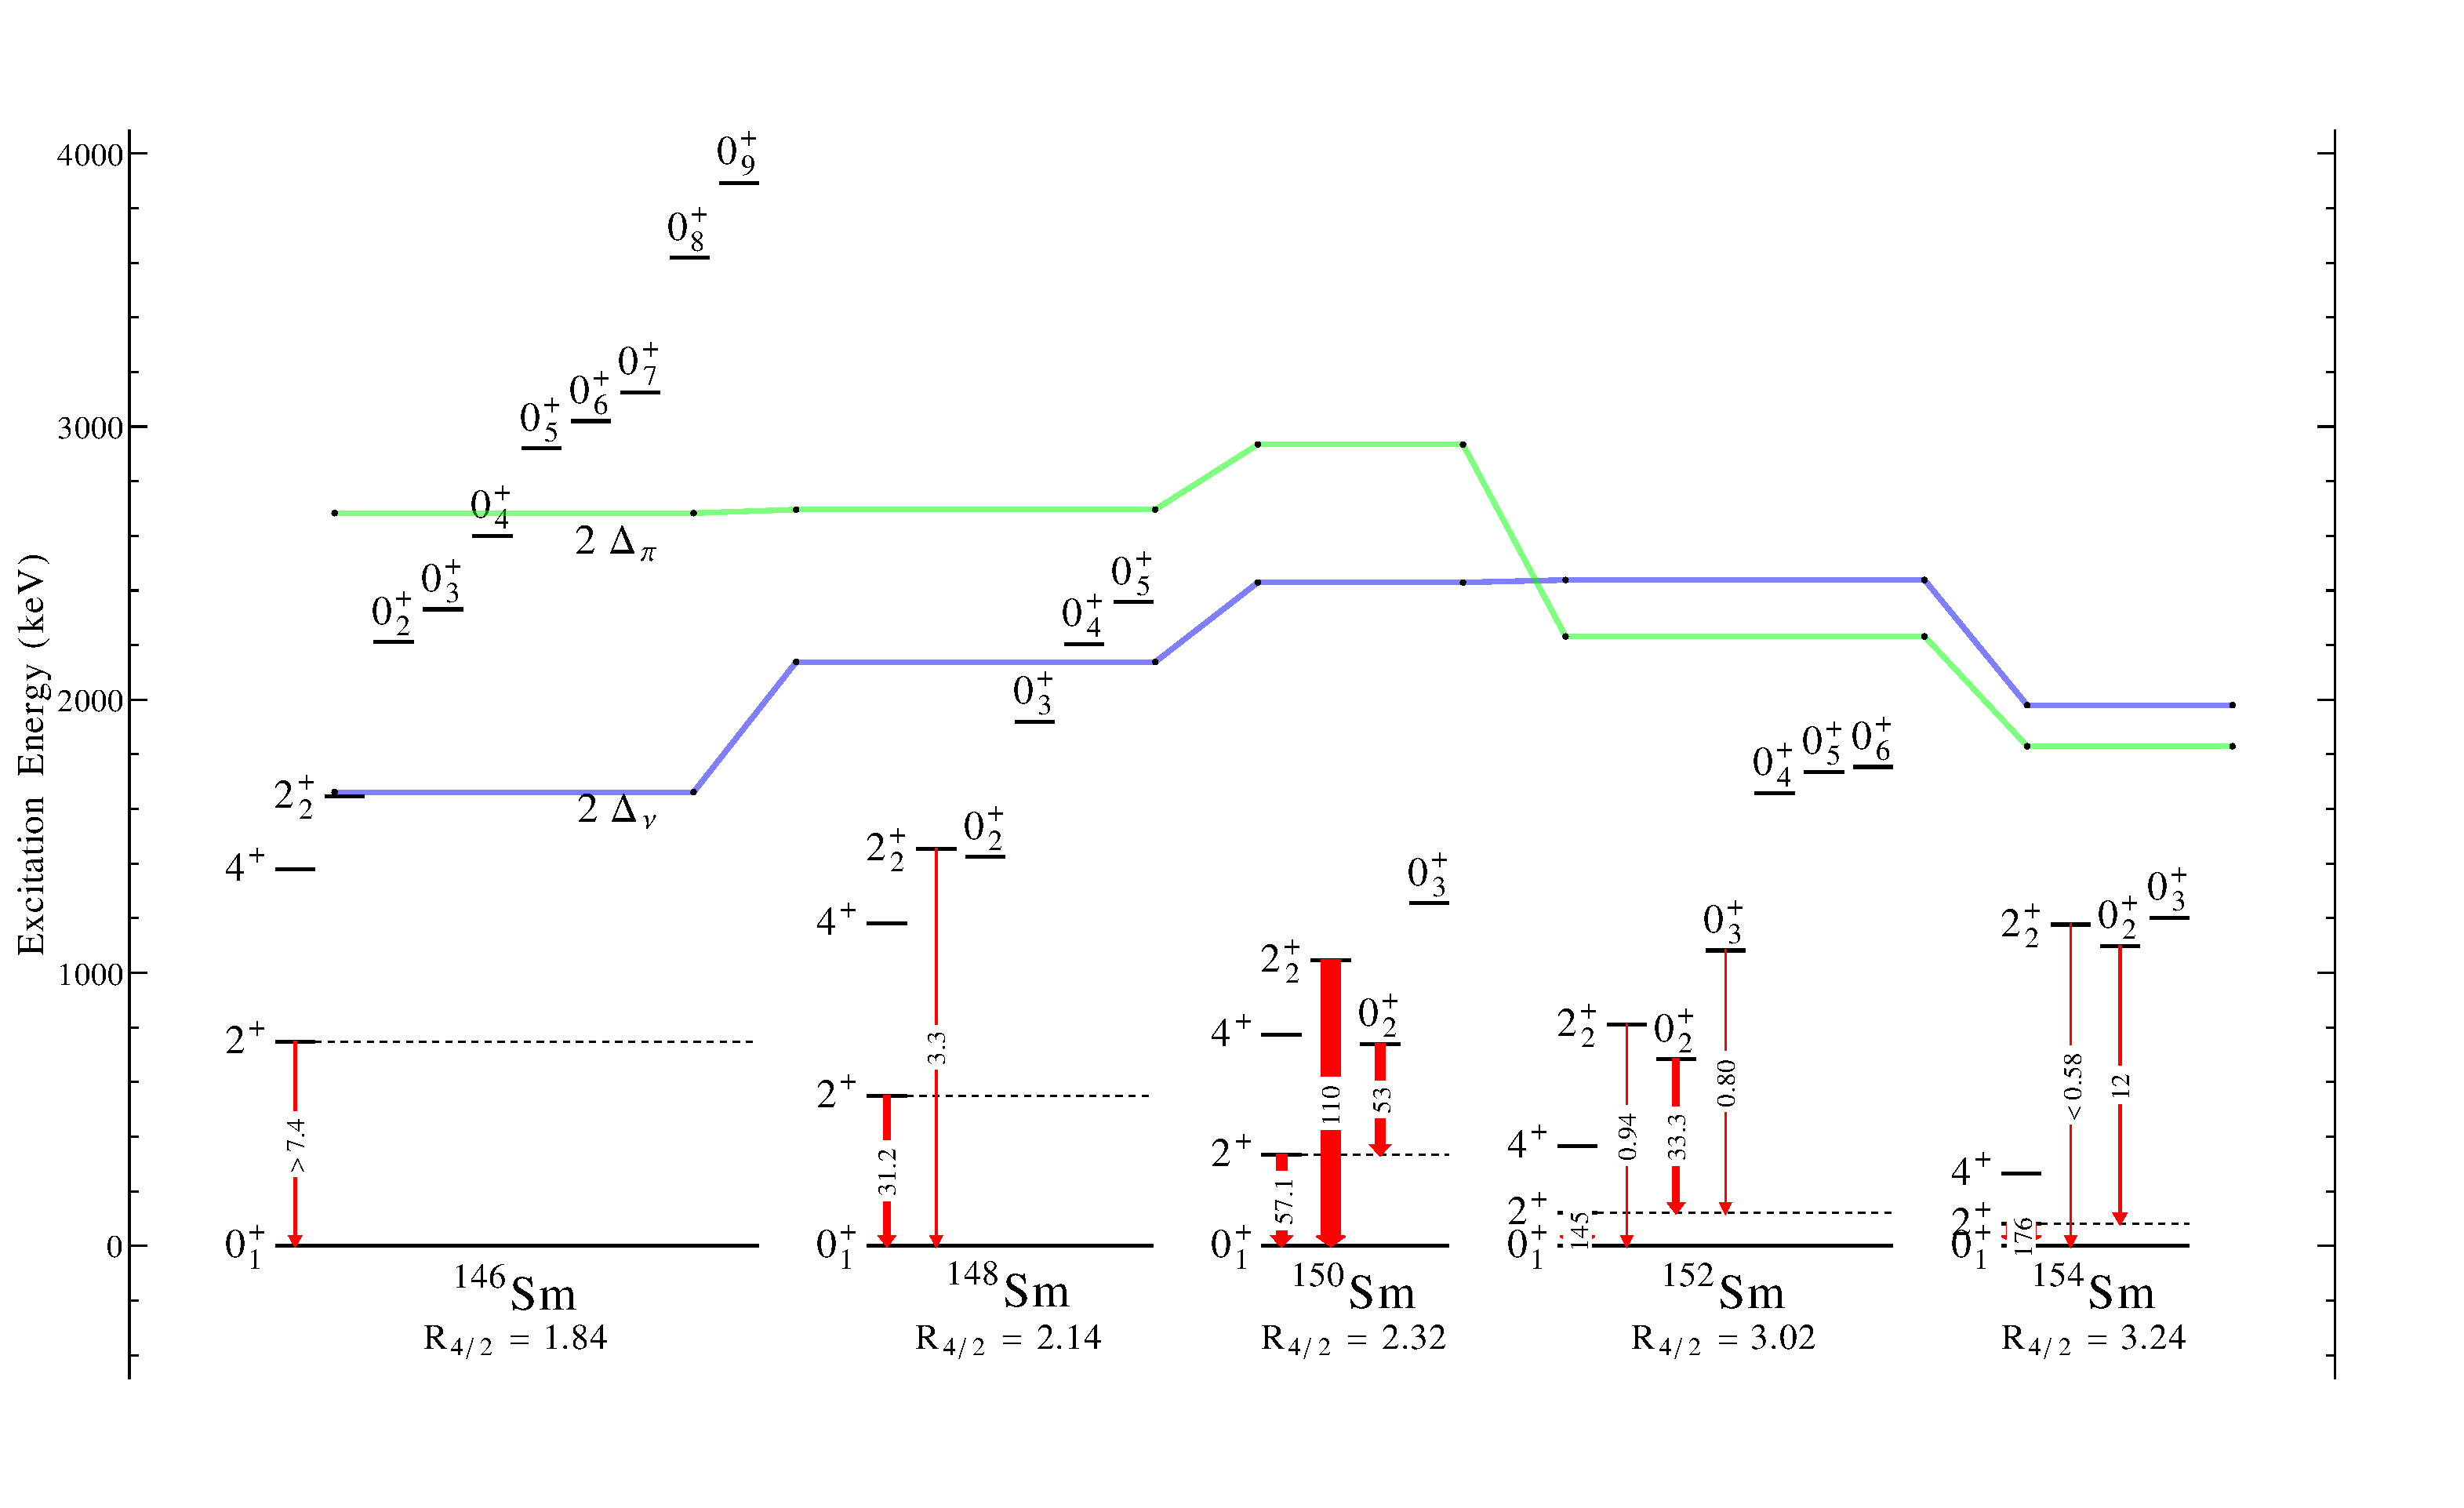
\includegraphics[height=0.8\textheight]{SciDraw_SmSystematics.pdf}
\caption{Systematics for the energies of excited 0$^+$ states, the first excited 2$^+$ bandhead, and low-lying ground state band members for even-even Samarium nuclei. Proton and neutron pairing gaps (2$\Delta_\pi$ and 2$\Delta_\nu$, respectively) are drawn in green and blue and are calculated from Equations \ref{eq:pairing_gapP} and \ref{eq:pairing_gapN}. Transition arrows represent known experimental B(E2) measurements for 0$^+$ bandheads and 2$^+$ bandheads (in W.u. where known).
\label{fig:SmSystematics}}
\end{center}
\end{figure}
\end{landscape}

% \subsection{K$^\pi$=0$^+$,2$^+$ systematics in Gadolinium Nuclei}

\begin{landscape}
\begin{figure}[ht] 
\begin{center}
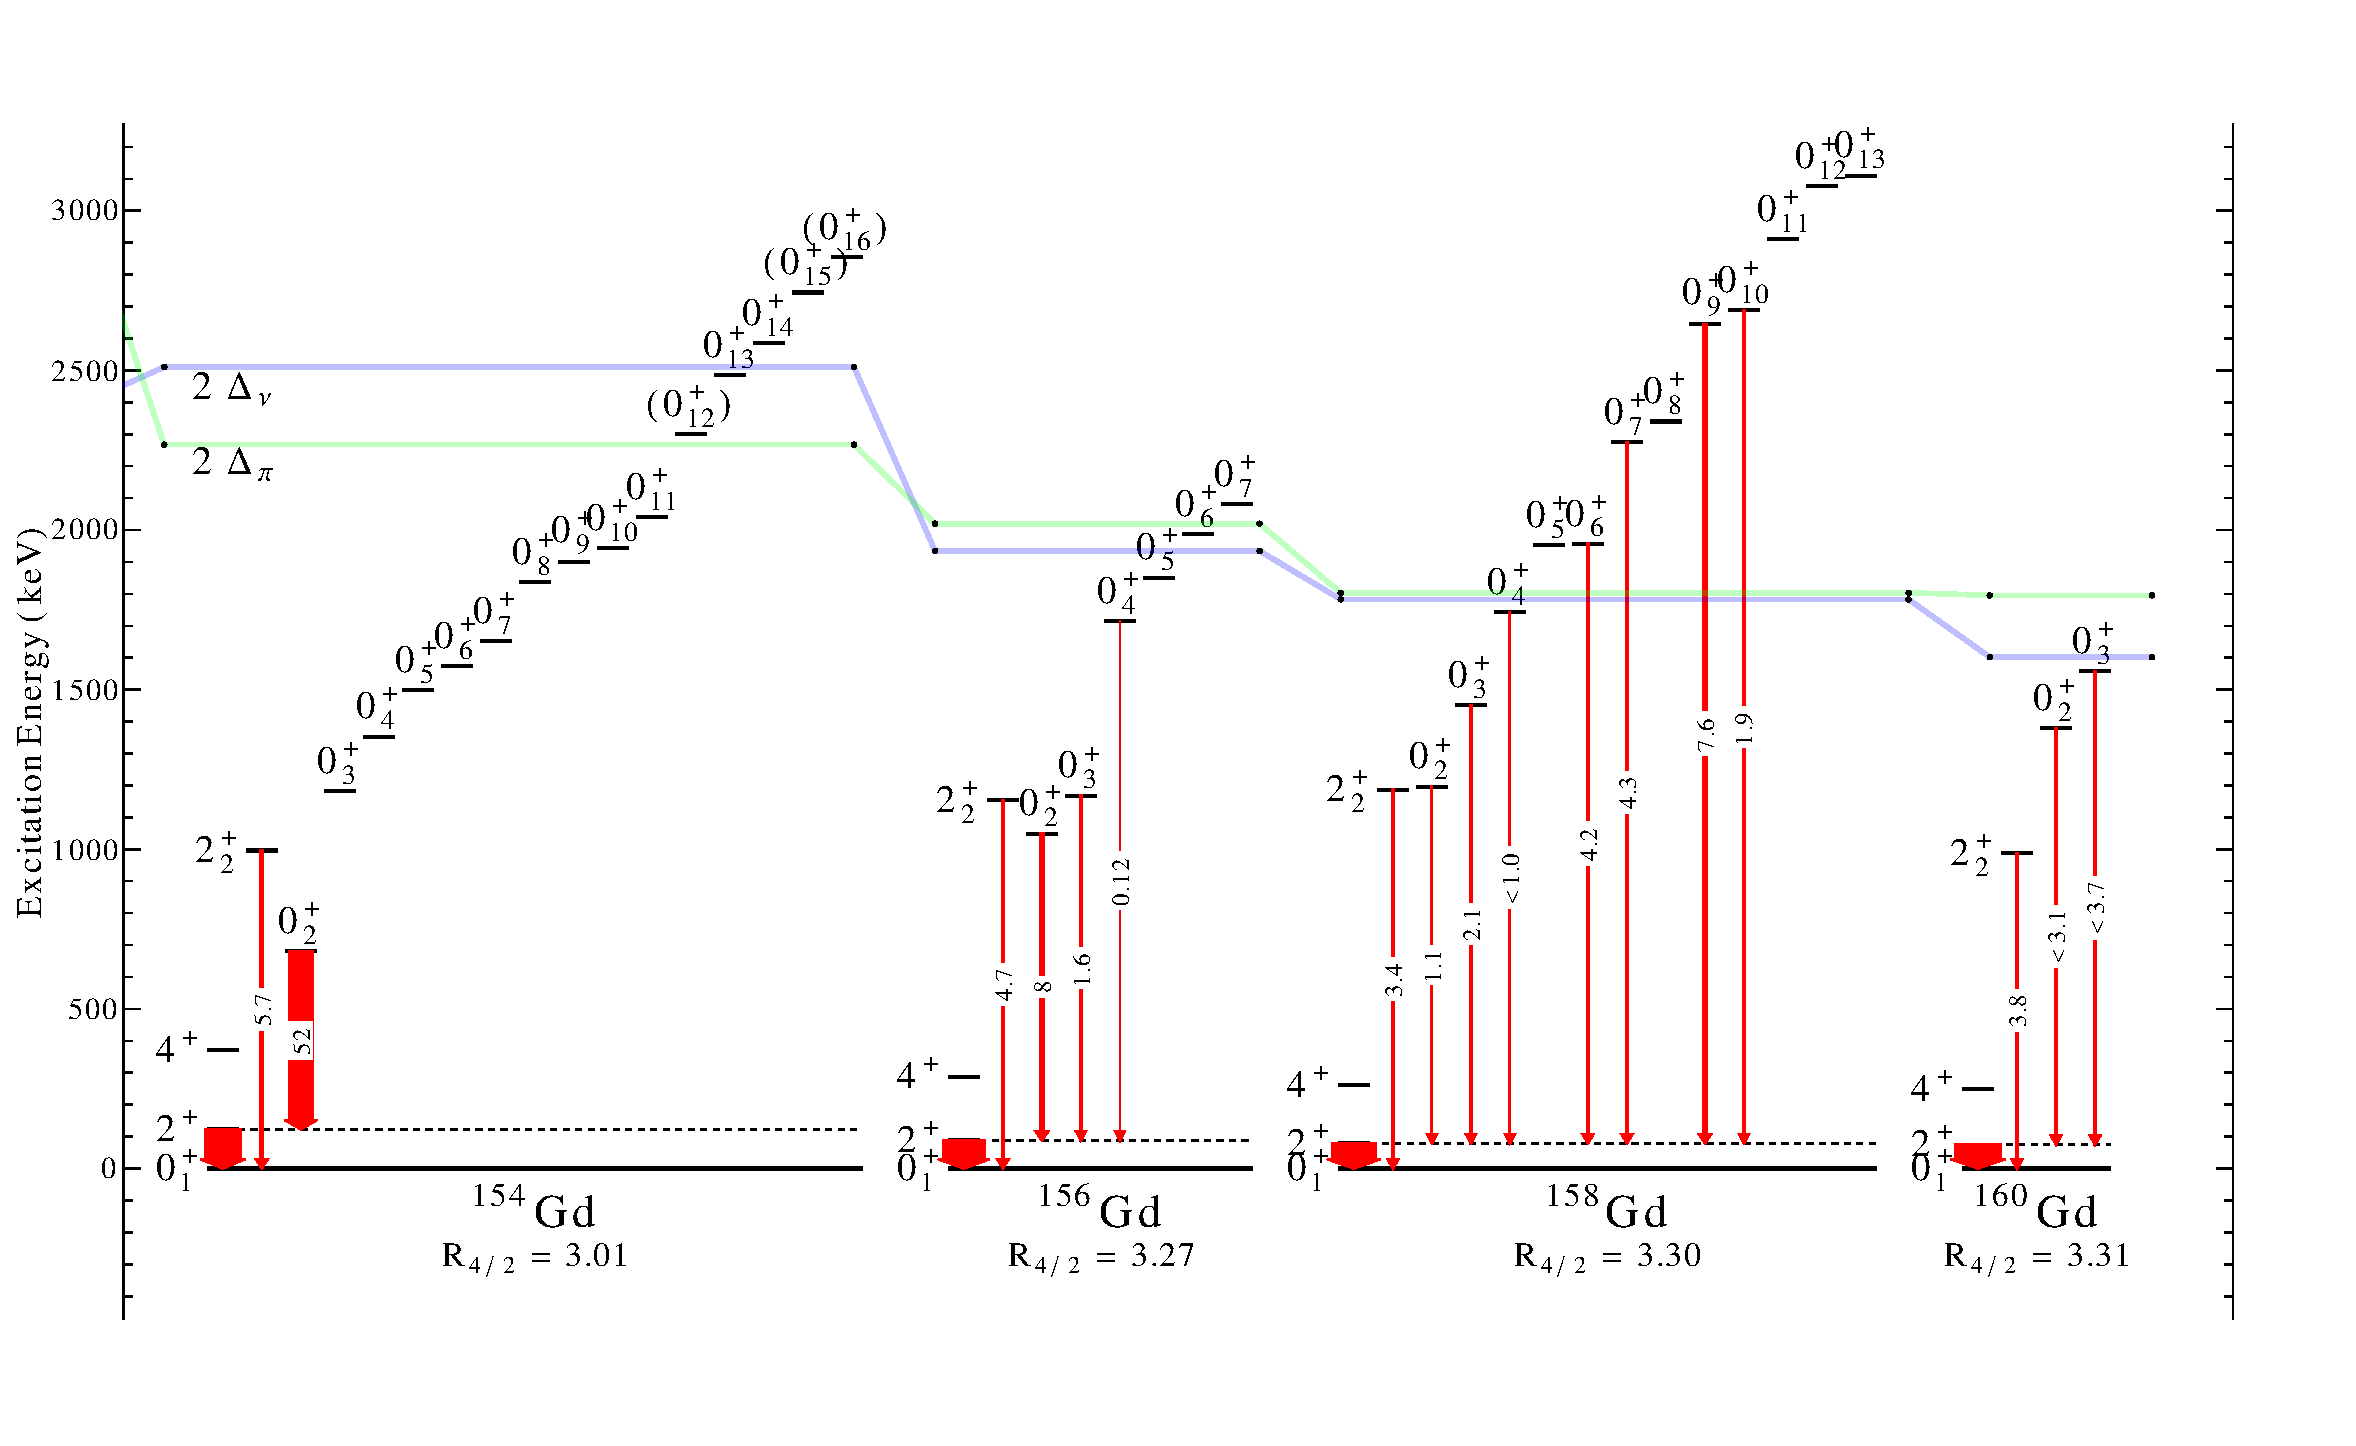
\includegraphics[height=0.8\textheight]{SciDraw_GdSystematics.pdf}
\caption{Systematics for the energies of excited 0$^+$ states, the first excited 2$^+$ bandhead, and low-lying ground state band members for even-even Gadolinium nuclei. Proton and neutron pairing gaps (2$\Delta_\pi$ and 2$\Delta_\nu$, respectively) are drawn in green and blue and are calculated from Equations \ref{eq:pairing_gapP} and \ref{eq:pairing_gapN}. Transition arrows represent known experimental B(E2) measurements for 0$^+$ bandheads and 2$^+$ bandheads (in W.u. where known).
\label{fig:GdSystematics}}
\end{center}
\end{figure}
\end{landscape}

% \subsection{K$^\pi$=0$^+$,2$^+$ systematics in Dysprosium Nuclei}

\begin{landscape}
\begin{figure}[ht] 
\begin{center}
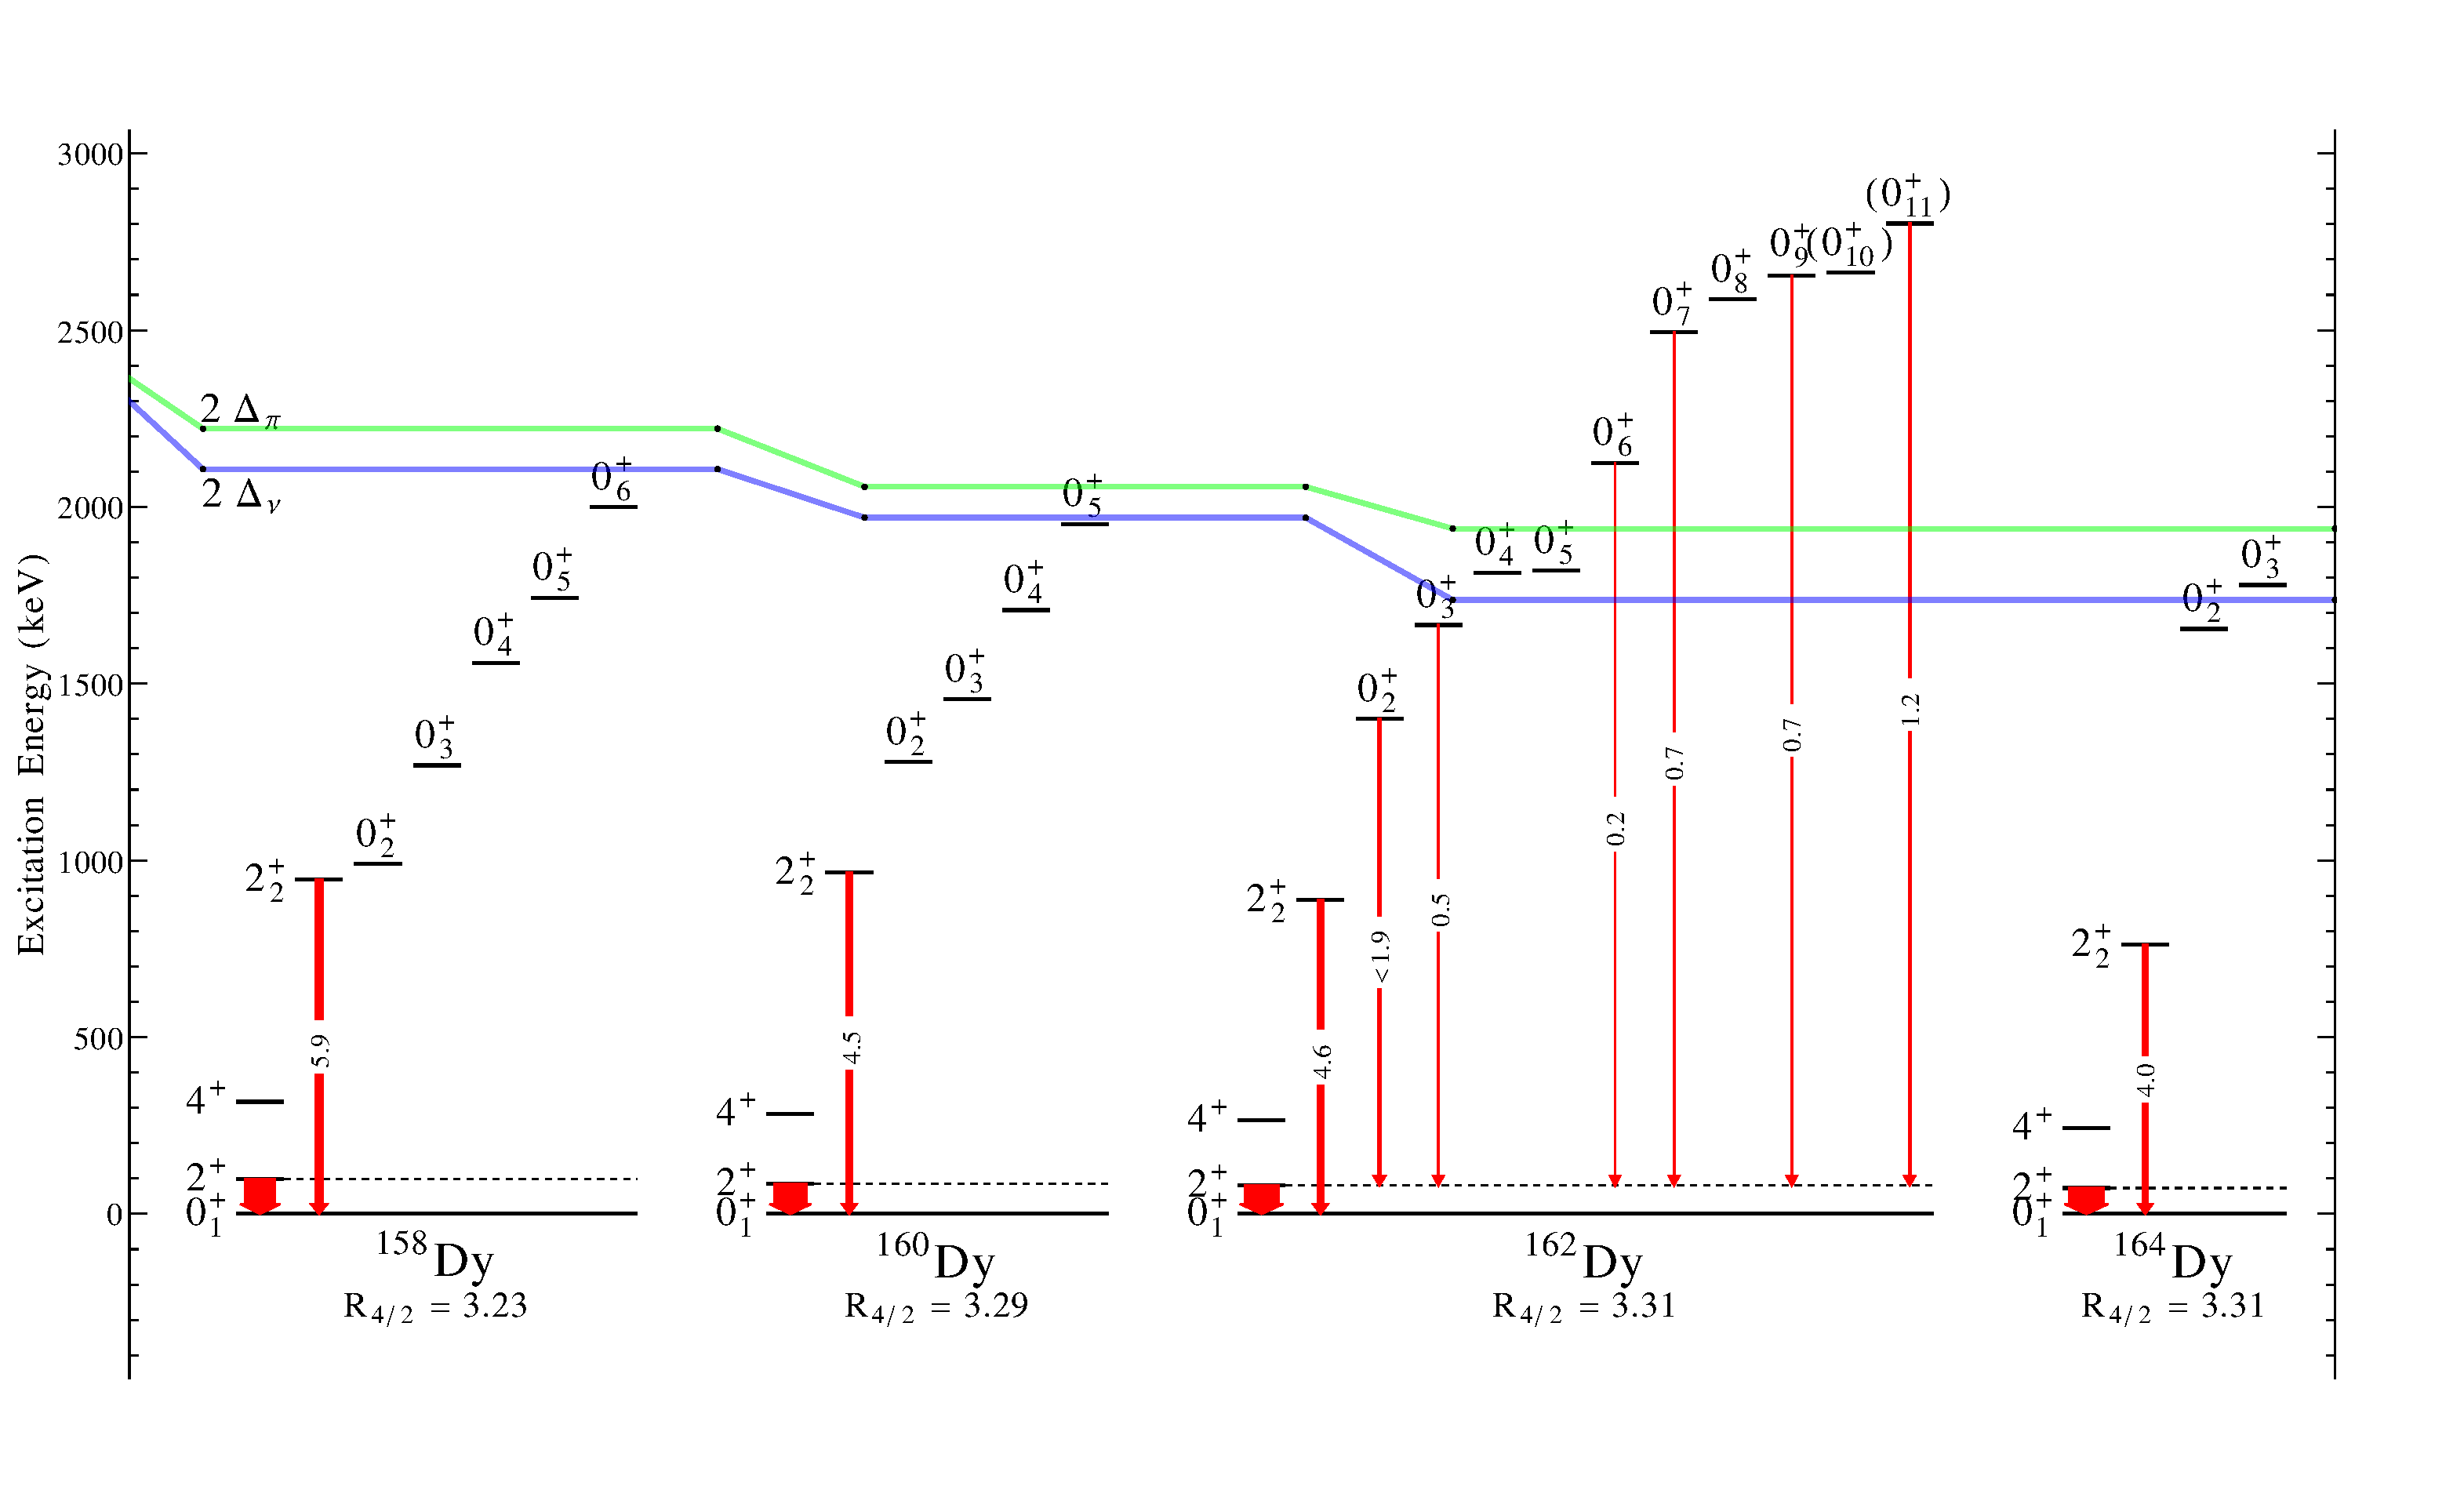
\includegraphics[height=0.8\textheight]{SciDraw_DySystematics.pdf}
\caption{Systematics for the energies of excited 0$^+$ states, the first excited 2$^+$ bandhead, and low-lying ground state band members for even-even Dysprosium nuclei. New transition probabilities are presented in $^{162}$Dy, with the widths proportional to B(E2) values (in W.u.); also shown are the proton and neutron pairing gap (2$\Delta_\pi$ and 2$\Delta_\nu$, respectively) for each isotope.
\label{fig:DySystematics}}
\end{center}
\end{figure}
\end{landscape}

\subsection{K$^\pi$=0$^+$,2$^+$ Systematics in Erbium, Ytterbium, and Hafnium Nuclei}
At the heavier end of the region, we echo some of the same rhetoric as the preceeding nuclei, in that lifetime information for all 0$^+$ states is lacking in select places, but we still retain \textit{some} semblance of the $\beta$-vibration in nuclei like $^{166}$Er and $^{172}$Hf, as well as an overall behavior of the $\gamma$ vibration across the entire chain of isotopes. In contrast, however, these nuclei are all well-deformed, and would be great nuclei to study the feasability of vibrations on top of deformed ground states (take $^{168}$Er for example).

\begin{landscape}
\begin{figure}[ht] 
\begin{center}
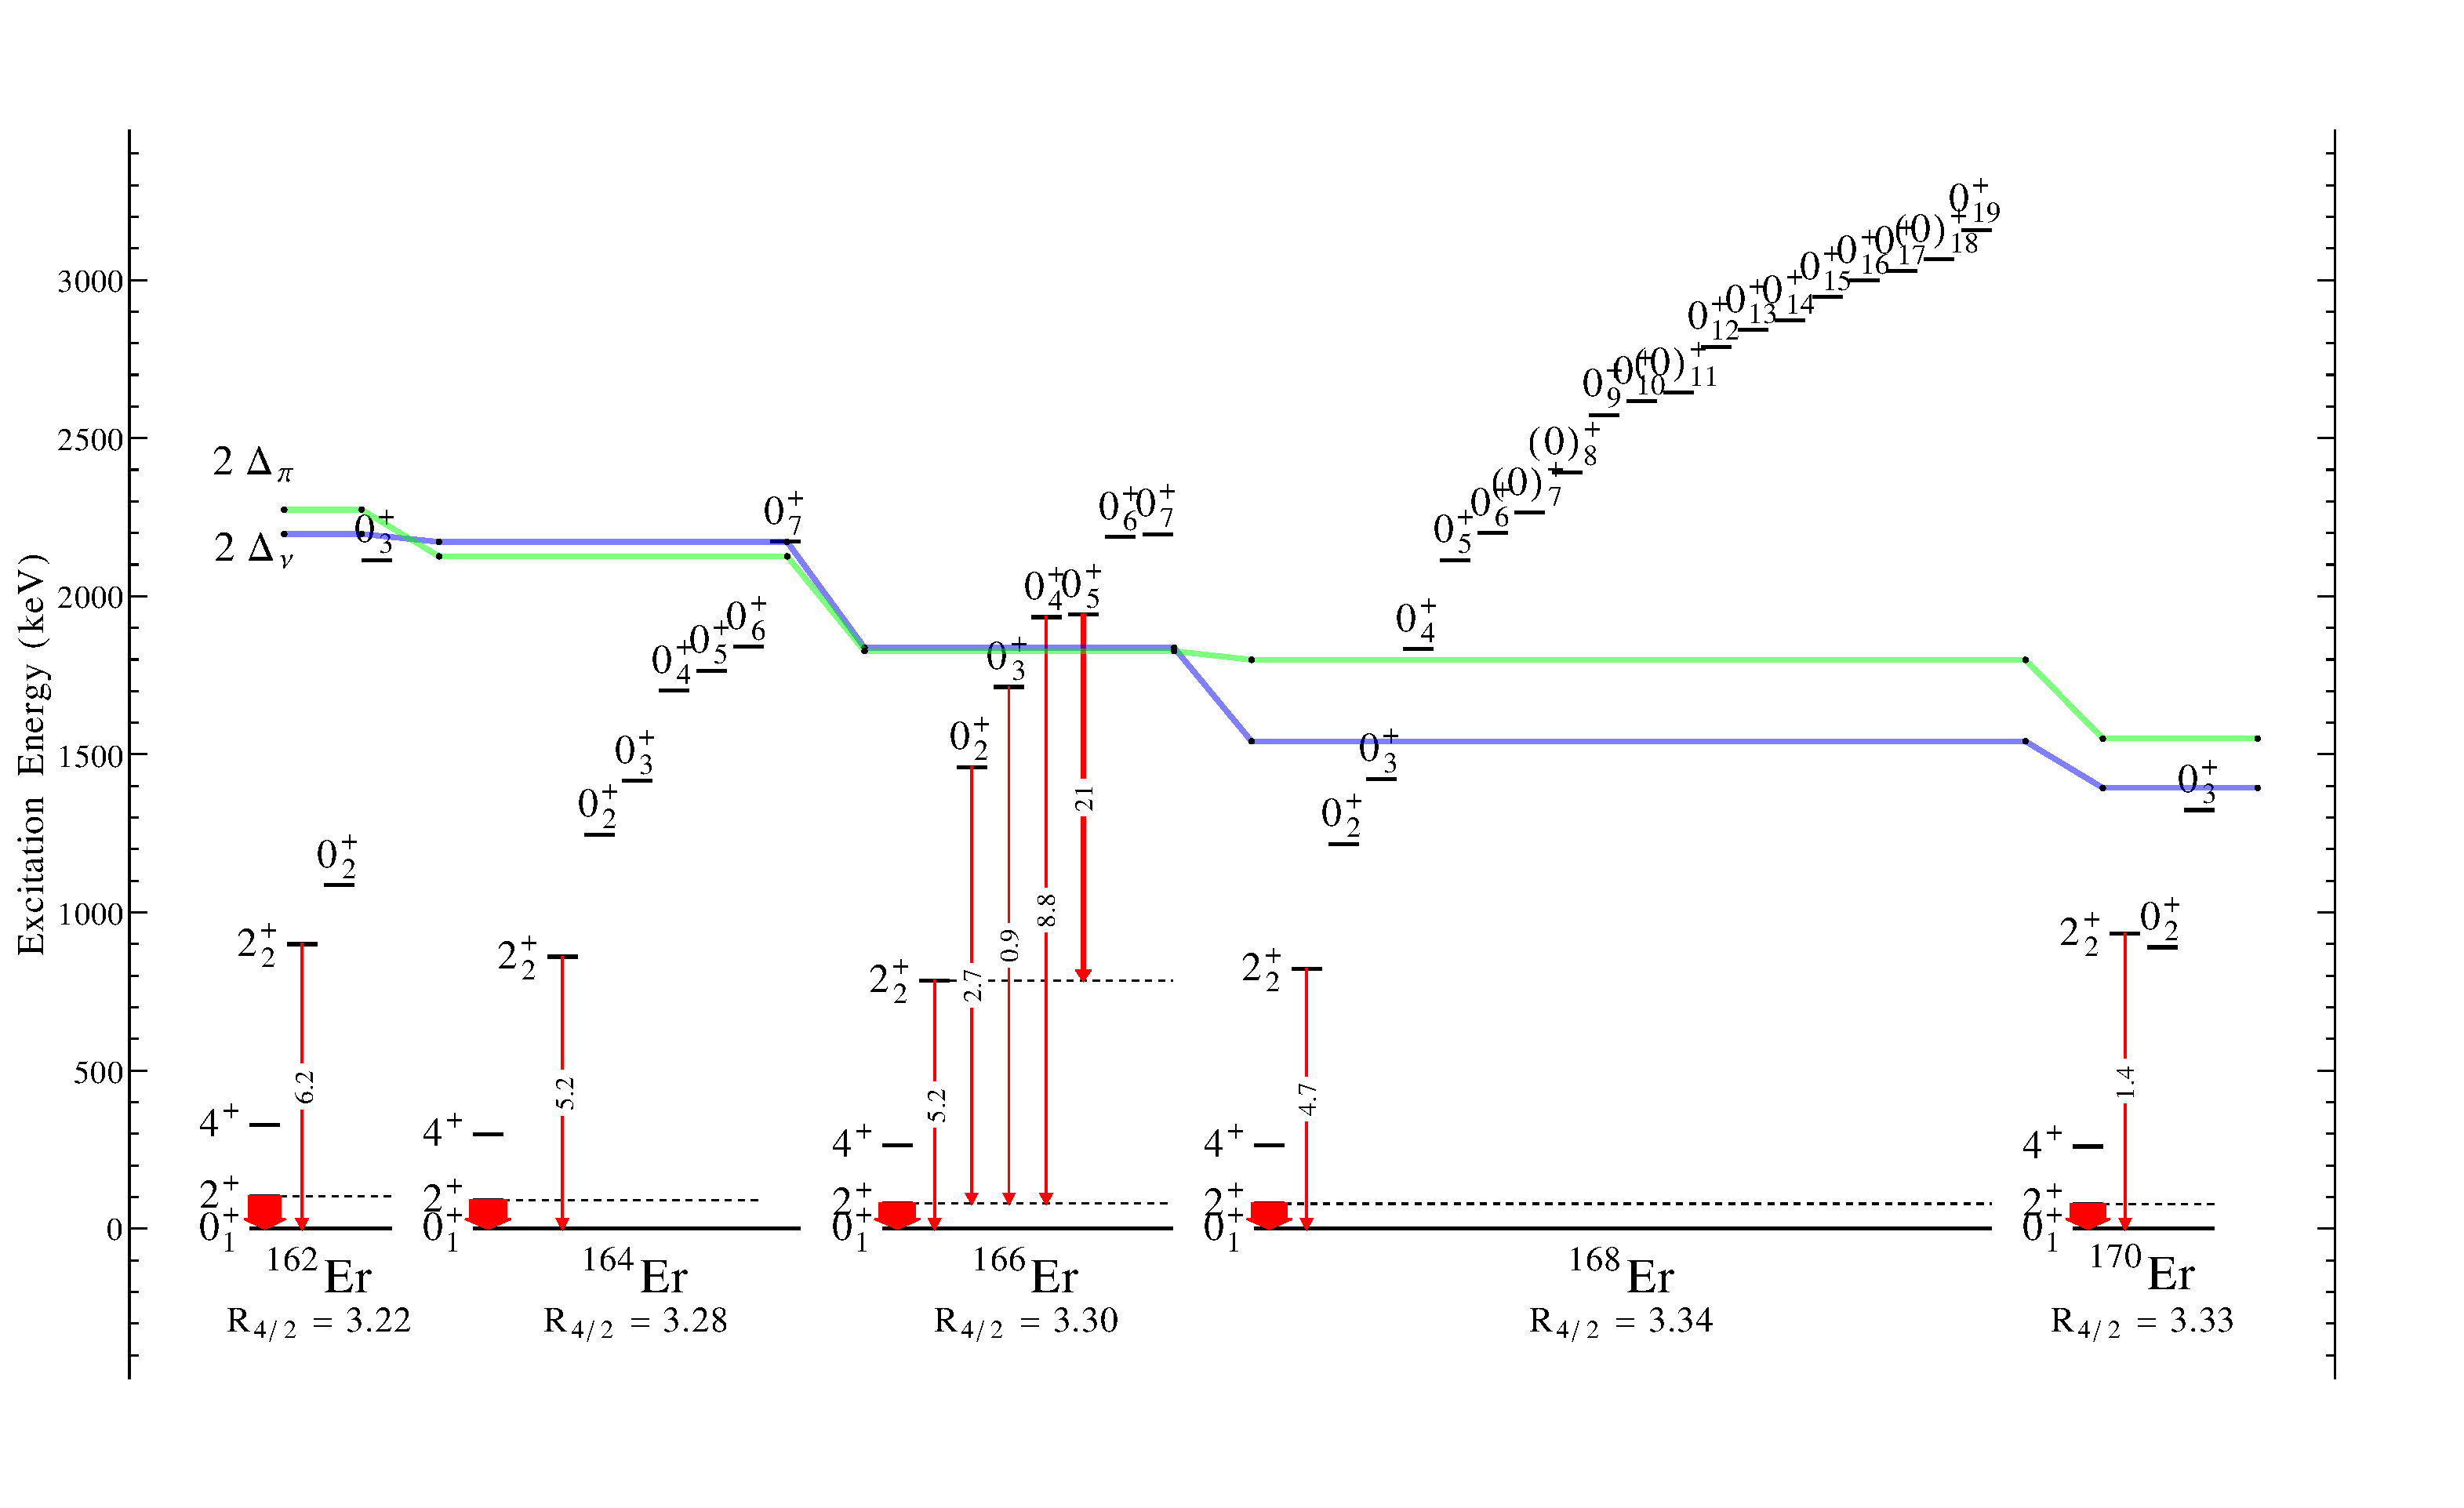
\includegraphics[height=0.8\textheight]{SciDraw_ErSystematics.pdf}
\caption{Systematics for the energies of excited 0$^+$ states, the first excited 2$^+$ bandhead, and low-lying ground state band members for even-even Erbium nuclei. Proton and neutron pairing gaps (2$\Delta_\pi$ and 2$\Delta_\nu$, respectively) are drawn in green and blue and are calculated from Equations \ref{eq:pairing_gapP} and \ref{eq:pairing_gapN}. Transition arrows represent known experimental B(E2) measurements for 0$^+$ bandheads and 2$^+$ bandheads (in W.u. where known).
\label{fig:ErSystematics}}
\end{center}
\end{figure}
\end{landscape}

% \subsection{K$^\pi$=0$^+$,2$^+$ systematics in Ytterbium Nuclei}
\begin{landscape}
\begin{figure}[ht] 
\begin{center}
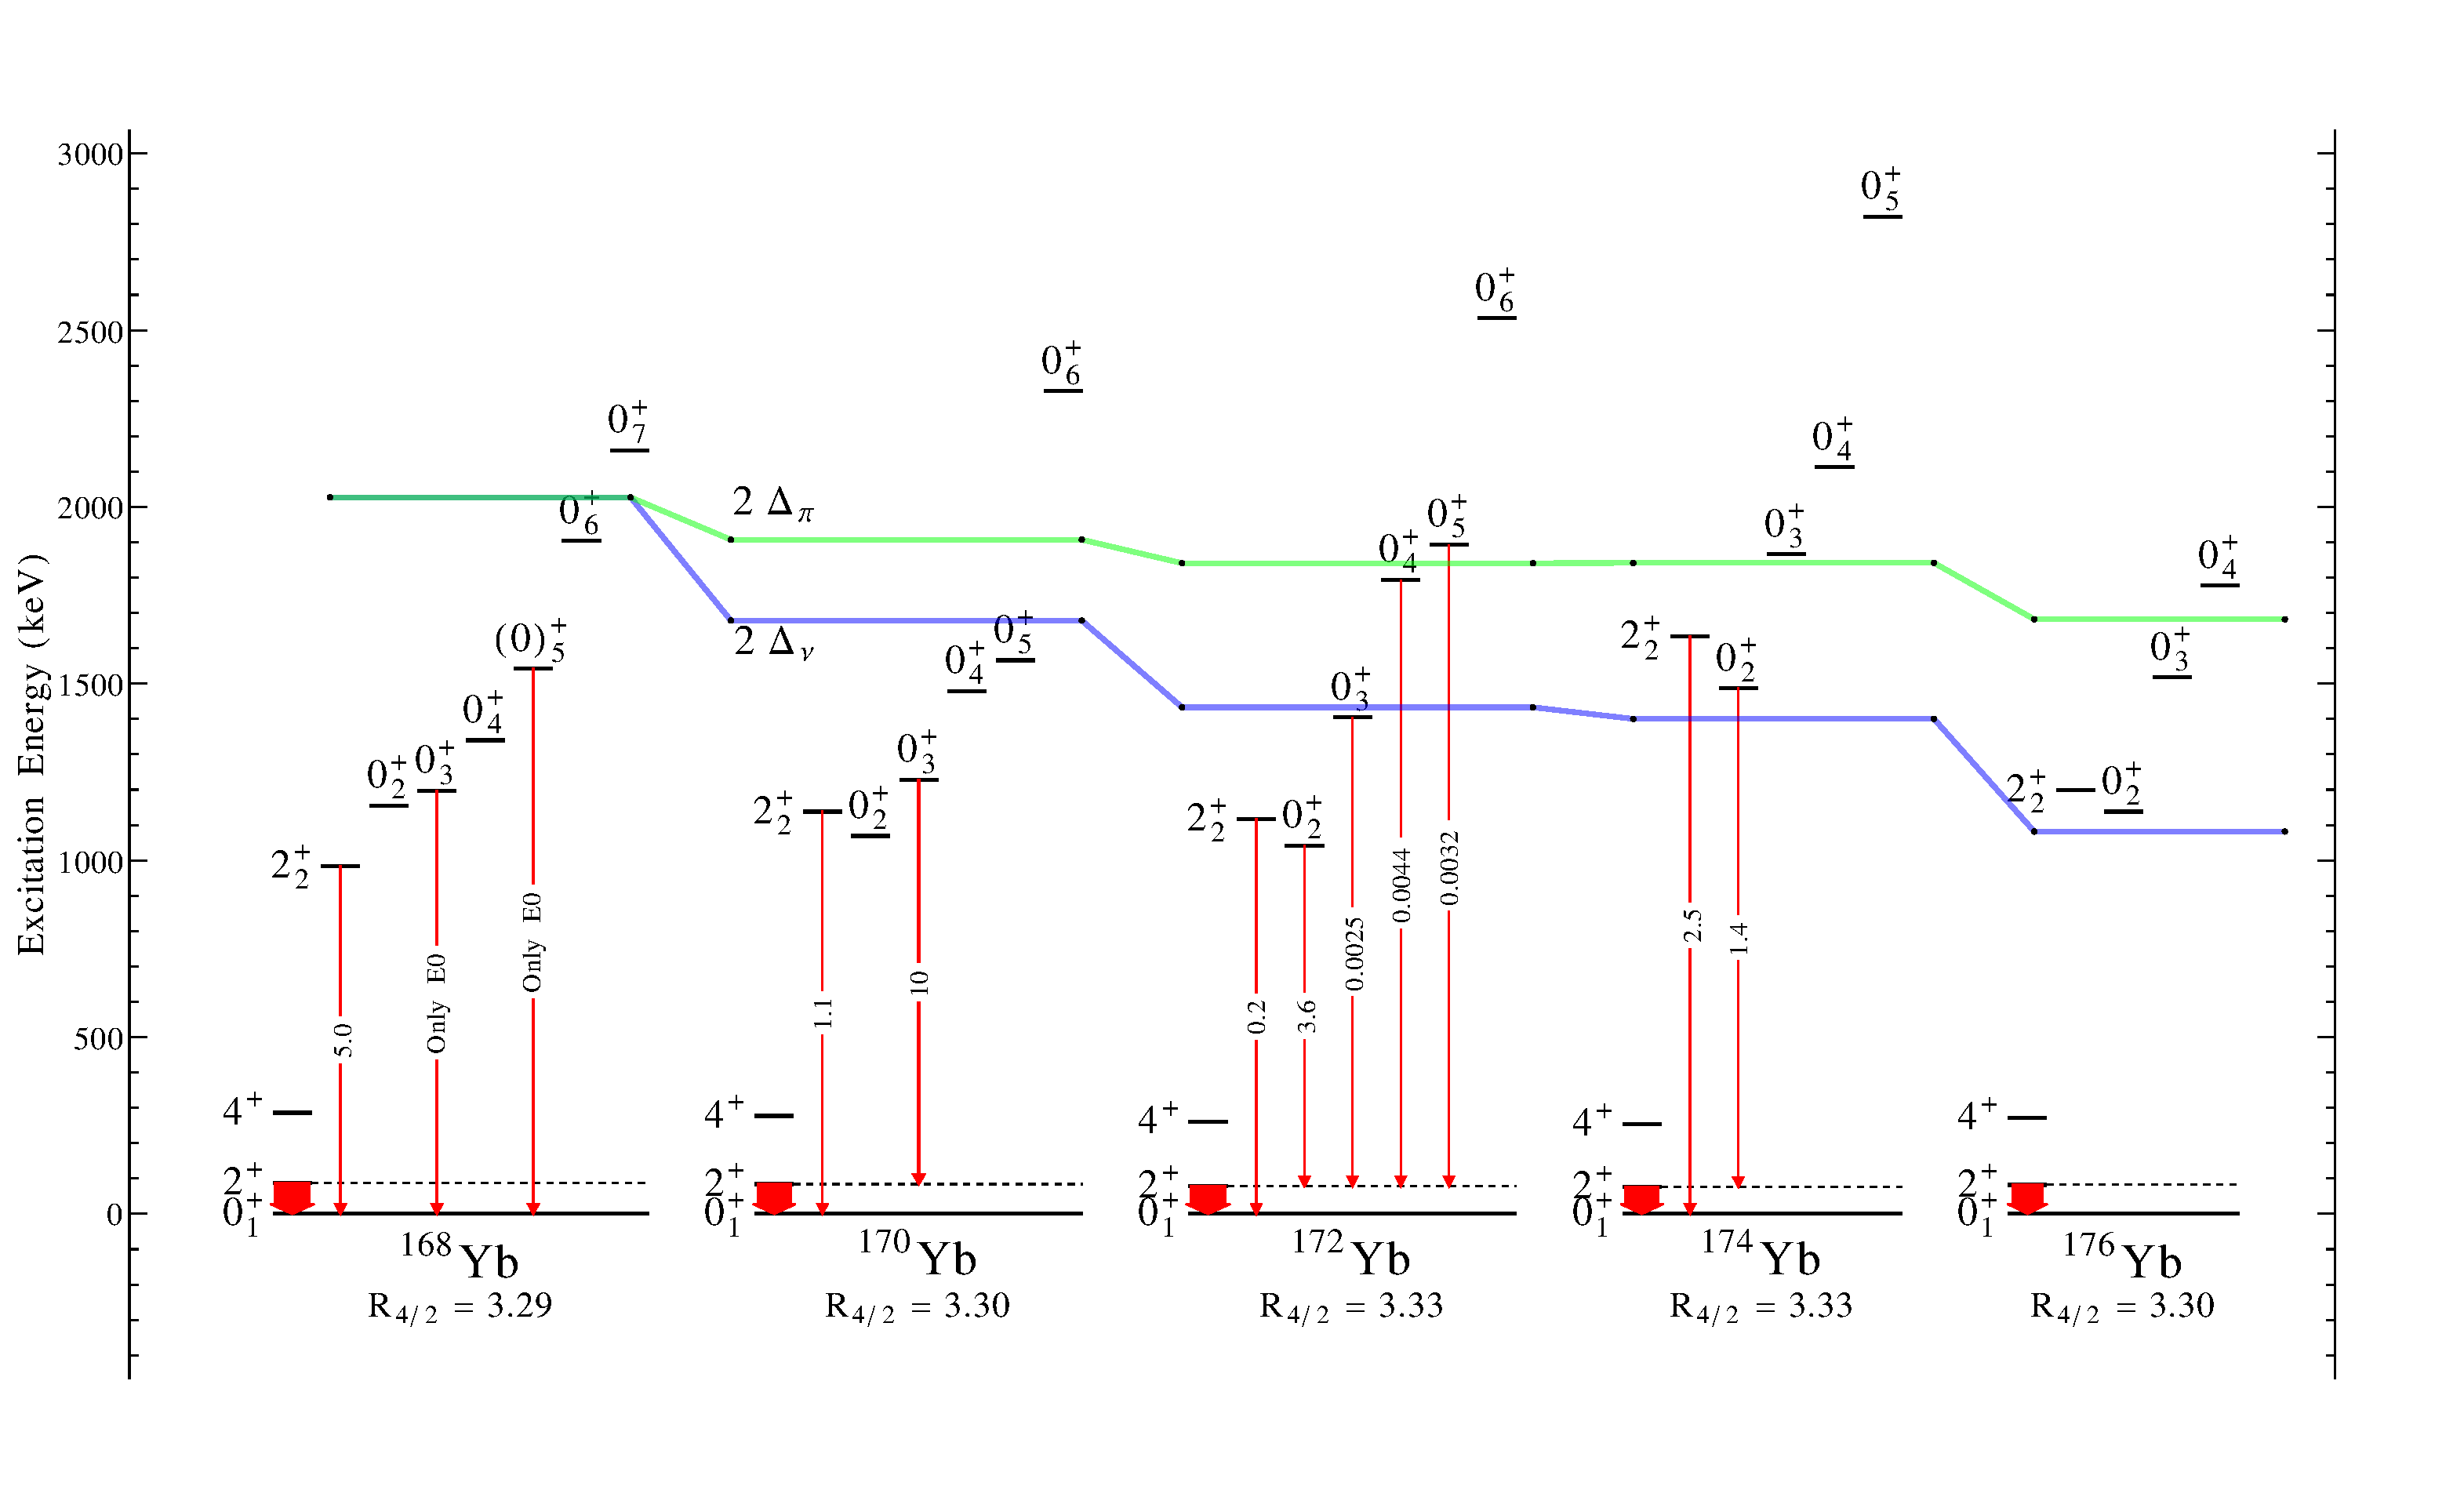
\includegraphics[height=0.8\textheight]{SciDraw_YbSystematics.pdf}
\caption{Systematics for the energies of excited 0$^+$ states, the first excited 2$^+$ bandhead, and low-lying ground state band members for even-even Ytterbium nuclei. Proton and neutron pairing gaps (2$\Delta_\pi$ and 2$\Delta_\nu$, respectively) are drawn in green and blue and are calculated from Equations \ref{eq:pairing_gapP} and \ref{eq:pairing_gapN}. Transition arrows represent known experimental B(E2) measurements for 0$^+$ bandheads and 2$^+$ bandheads (in W.u. where known).
\label{fig:YbSystematics}}
\end{center}
\end{figure}
\end{landscape}
% \subsection{K$^\pi$=0$^+$,2$^+$ systematics in Hafnium Nuclei}

\begin{landscape}
\begin{figure}[ht] 
\begin{center}
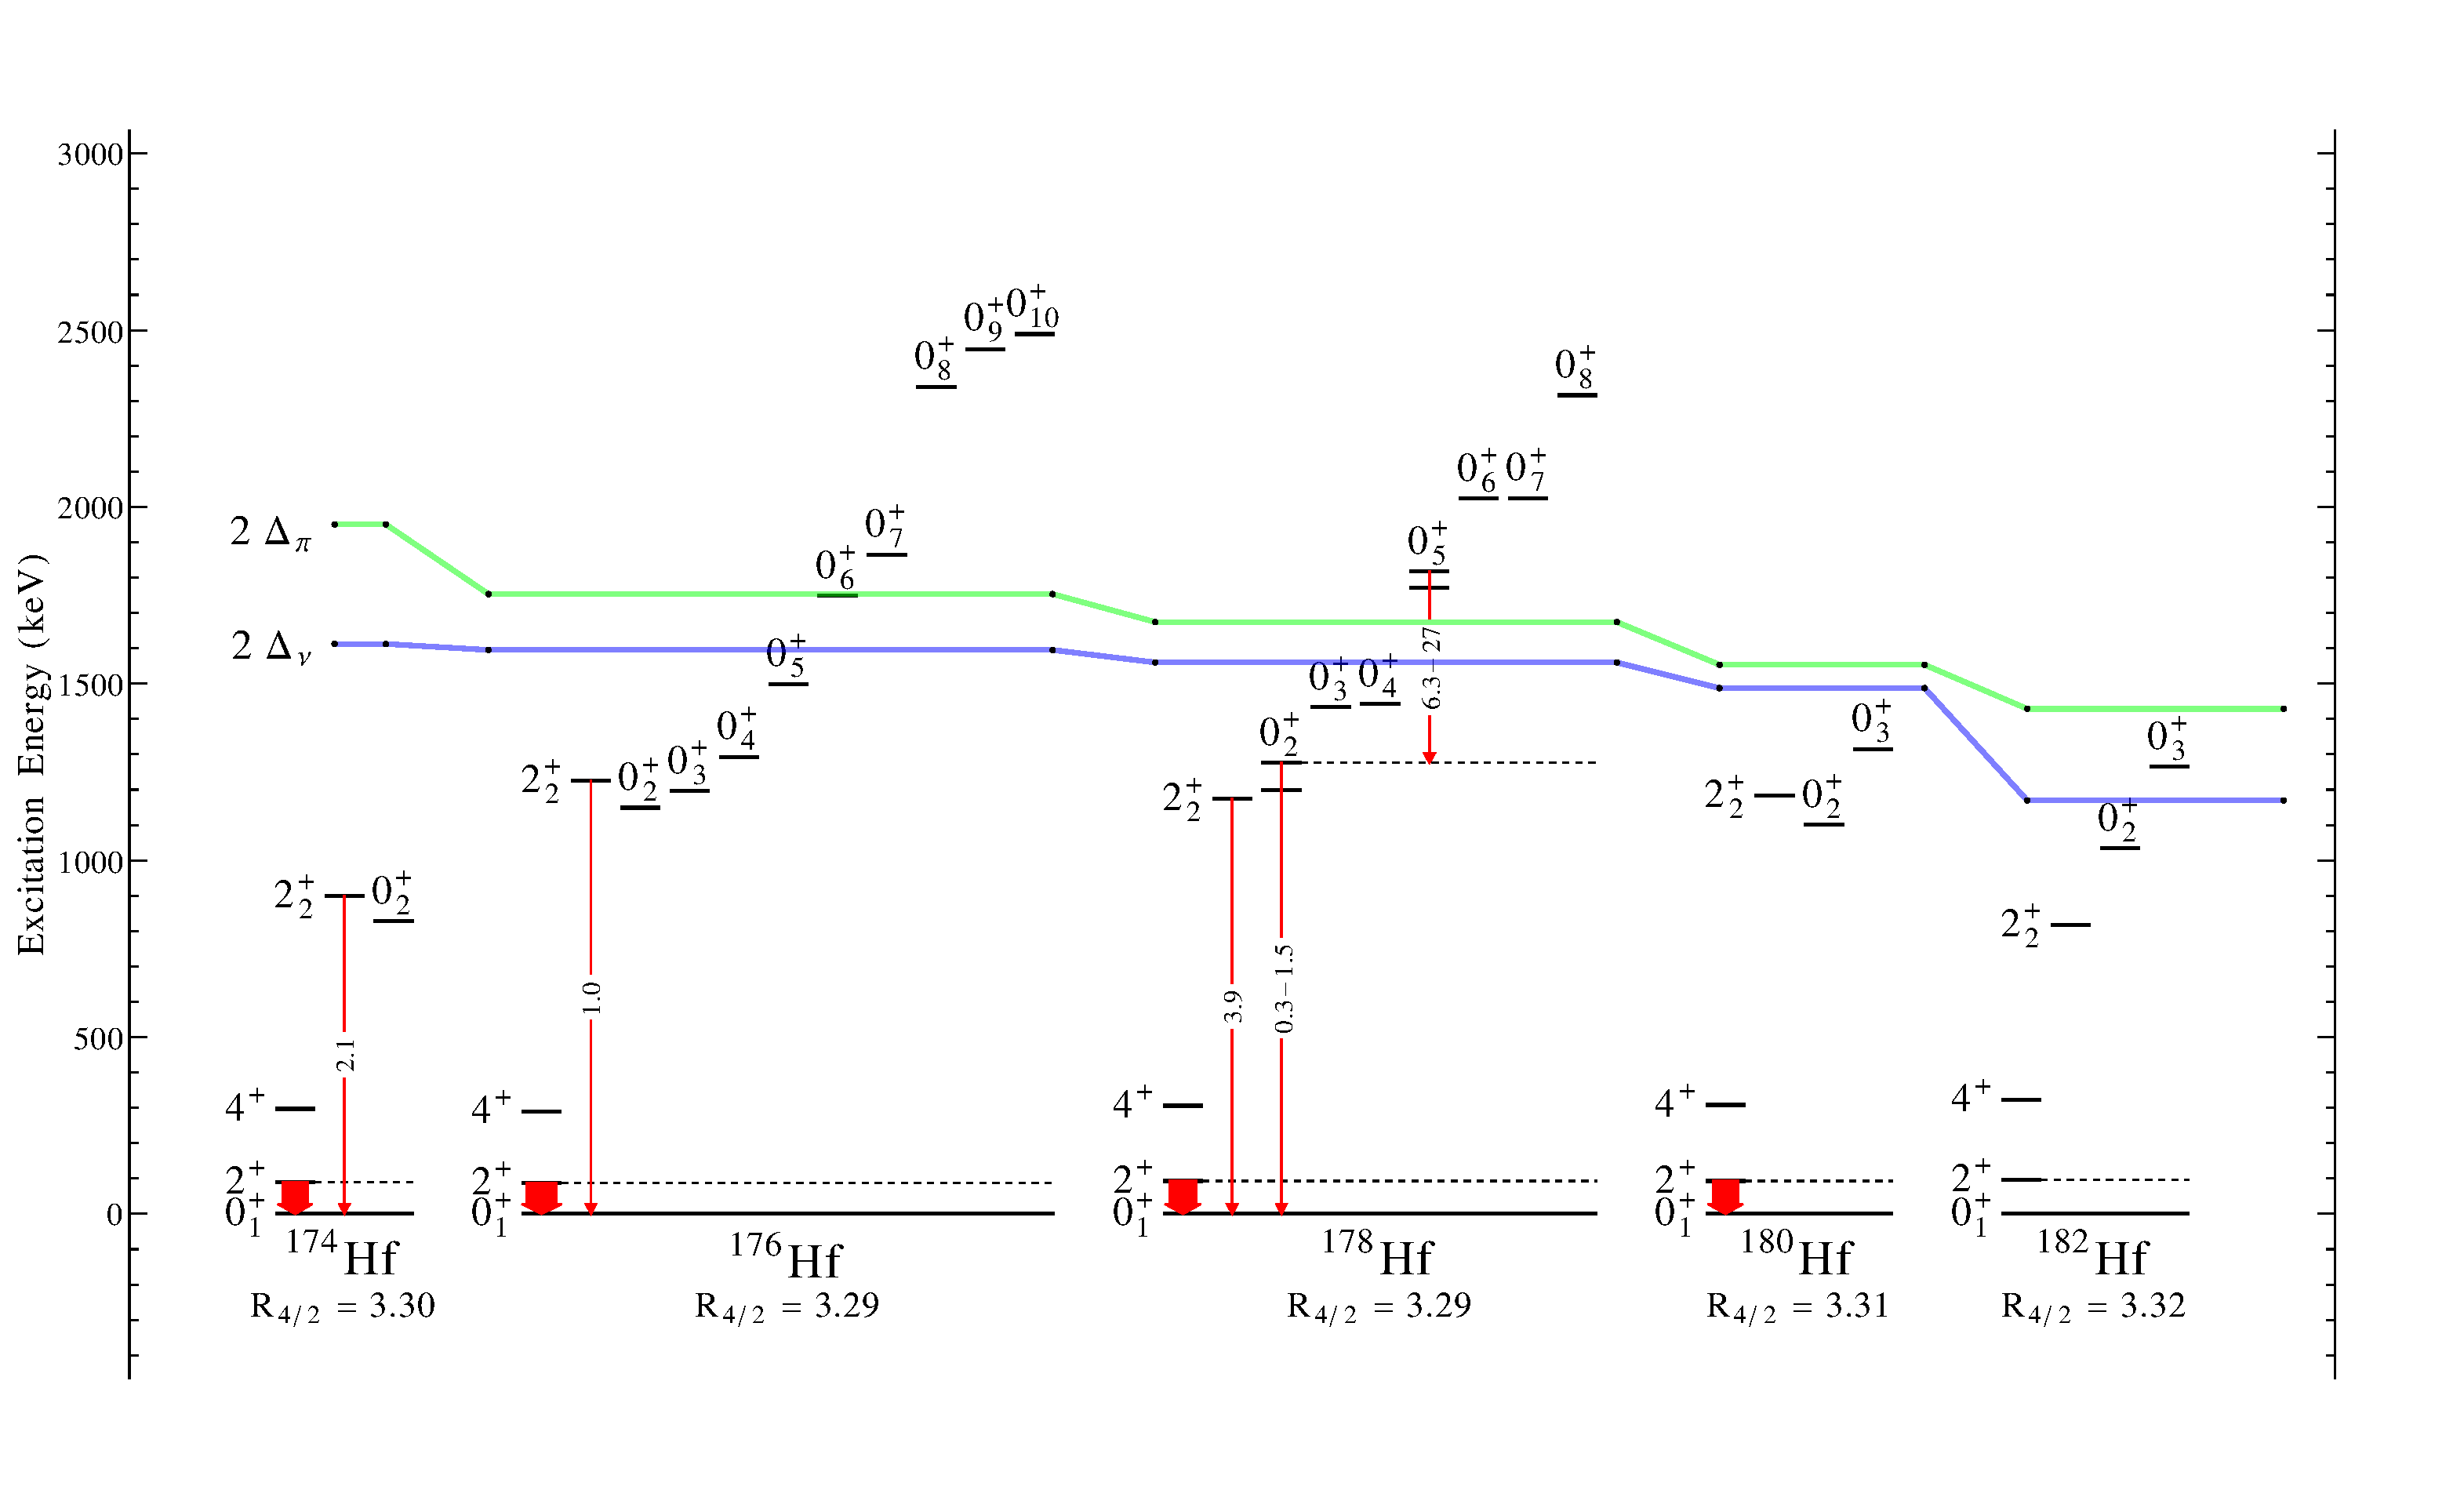
\includegraphics[height=0.8\textheight]{SciDraw_HfSystematics.pdf}
\caption{Systematics for the energies of excited 0$^+$ states, the first excited 2$^+$ bandhead, and low-lying ground state band members for even-even Hafnium nuclei. Proton and neutron pairing gaps (2$\Delta_\pi$ and 2$\Delta_\nu$, respectively) are drawn in green and blue and are calculated from Equations \ref{eq:pairing_gapP} and \ref{eq:pairing_gapN}. Transition arrows represent known experimental B(E2) measurements for 0$^+$ bandheads and 2$^+$ bandheads (in W.u. where known).
\label{fig:HfSystematics}}
\end{center}
\end{figure}
\end{landscape}

In these figures, we can immediately observe some key motivations for performing lifetime measurements in the rare earth region. First, there are currently pockets where we lack literature lifetime information for 0$^+$ excitations in the 150$<$A$<$180 region, especially for states below the proton and neutron pairing gaps, where we would expect to find macroscopic collective motion. Second, in the Gadolinium nuclei, a particular suppression of the collectivity of the lowest-lying 0$^+$ state appears as the static deformation increases. This decrease in collective strength complements the long-standing irregularities in collective strength of 0$^+$ excitations, highlighted by the otherwise `well-behaved' collectivity of the lowest lying K$^\pi$=2$^+$ bands \cite{Casten_0plusbehavior2005, Bonatsos_collective02009}. Lastly, this general inconsistency in collective strength of the 0$^+$ states must be further investigated (previous studies include \cite{Sharpey-Schafer2011,SharpeySchafer_beta2011,Garrett_02_beta}) to match the assertions provided in \cite{RevModPhys.83.1467}. It is entirely reasonable to make the case for strongly collective $\beta$-vibrations in spherical or transitionally deformed nuclei with strong B(E2)s to the ground state 2$^+$, (see $^{150,152}$Sm in Figure \ref{fig:SmSystematics} and $^{154}$Gd in \ref{fig:GdSystematics}) where R$_{\frac{4}{2}}<$3, but as we move to the well-deformed, rotational limit of nuclei, the story definitively changes, and the behavior of the lowest-lying 0$^+$ state changes drastically! Nuclei in the rare-earth region along the line of stability have been hallmarks of spectroscopic knowledge, being some of the most well-studied nuclei for decades, giving us a well-defined goal to characterize the multitude of states where we have a wealth of knowledge as a foundation!

%We also see the various double-phonon cases of 166Er and 178Hf, yet these excitations are only a few in the vast sea of 0+ excitations in rare-earth nuclei. 









\subsection{Negative Parity States in Gadolinium and Dysprosium Nuclei}


We can also see the lack of lifetime information for low-lying negative parity states in rare-earth nuclei, of which, we will study the same cases ($^{160}$Gd and $^{162}$Dy) for the isotopic chains of even-even rare-earth nuclei. Figures \ref{fig:GdSystematics_Octupole} and \ref{fig:DySystematics_Octupole} show the energy systematics for the lowest-lying negative parity bands across isotopes. Immediately again, we see the enegies of the negative parity states mentioned in \S \ref{sec:excitedstates} in regards to the shifting and re-ordering of the split negative parity bands. Again, just like the K$^\pi$=0$^+$ bands, crucial lifetime information for these states is scarce (only 6 lifetimes of negative parity states are known in Dysprosium nuclei); given the number of excitations below the pairing gap (where we expect to see collective excitations), measurement of the B(E1) transition probabilities can allude to any octupole correlations as a phonon excitation in the nuclei discussed in this work, yet the most important piece of experimental evidence (which still remains out of the scope of the experiments performed in this work) is the absolute B(E3) transition probabilities linking states. Enhanced B(E1) strengths have been attributed to the octupole vibration as a type of reflection asymmetry, but are not a smoking gun of the octupole vibration, but more and more nuclei in the rare-earth region display an enhanced degree of dipole strength in the octupole vibration \cite{Soloviev_QuadHex,Pascu_octupole_2015}. 

\begin{landscape}
\begin{figure}[ht] 
\begin{center}
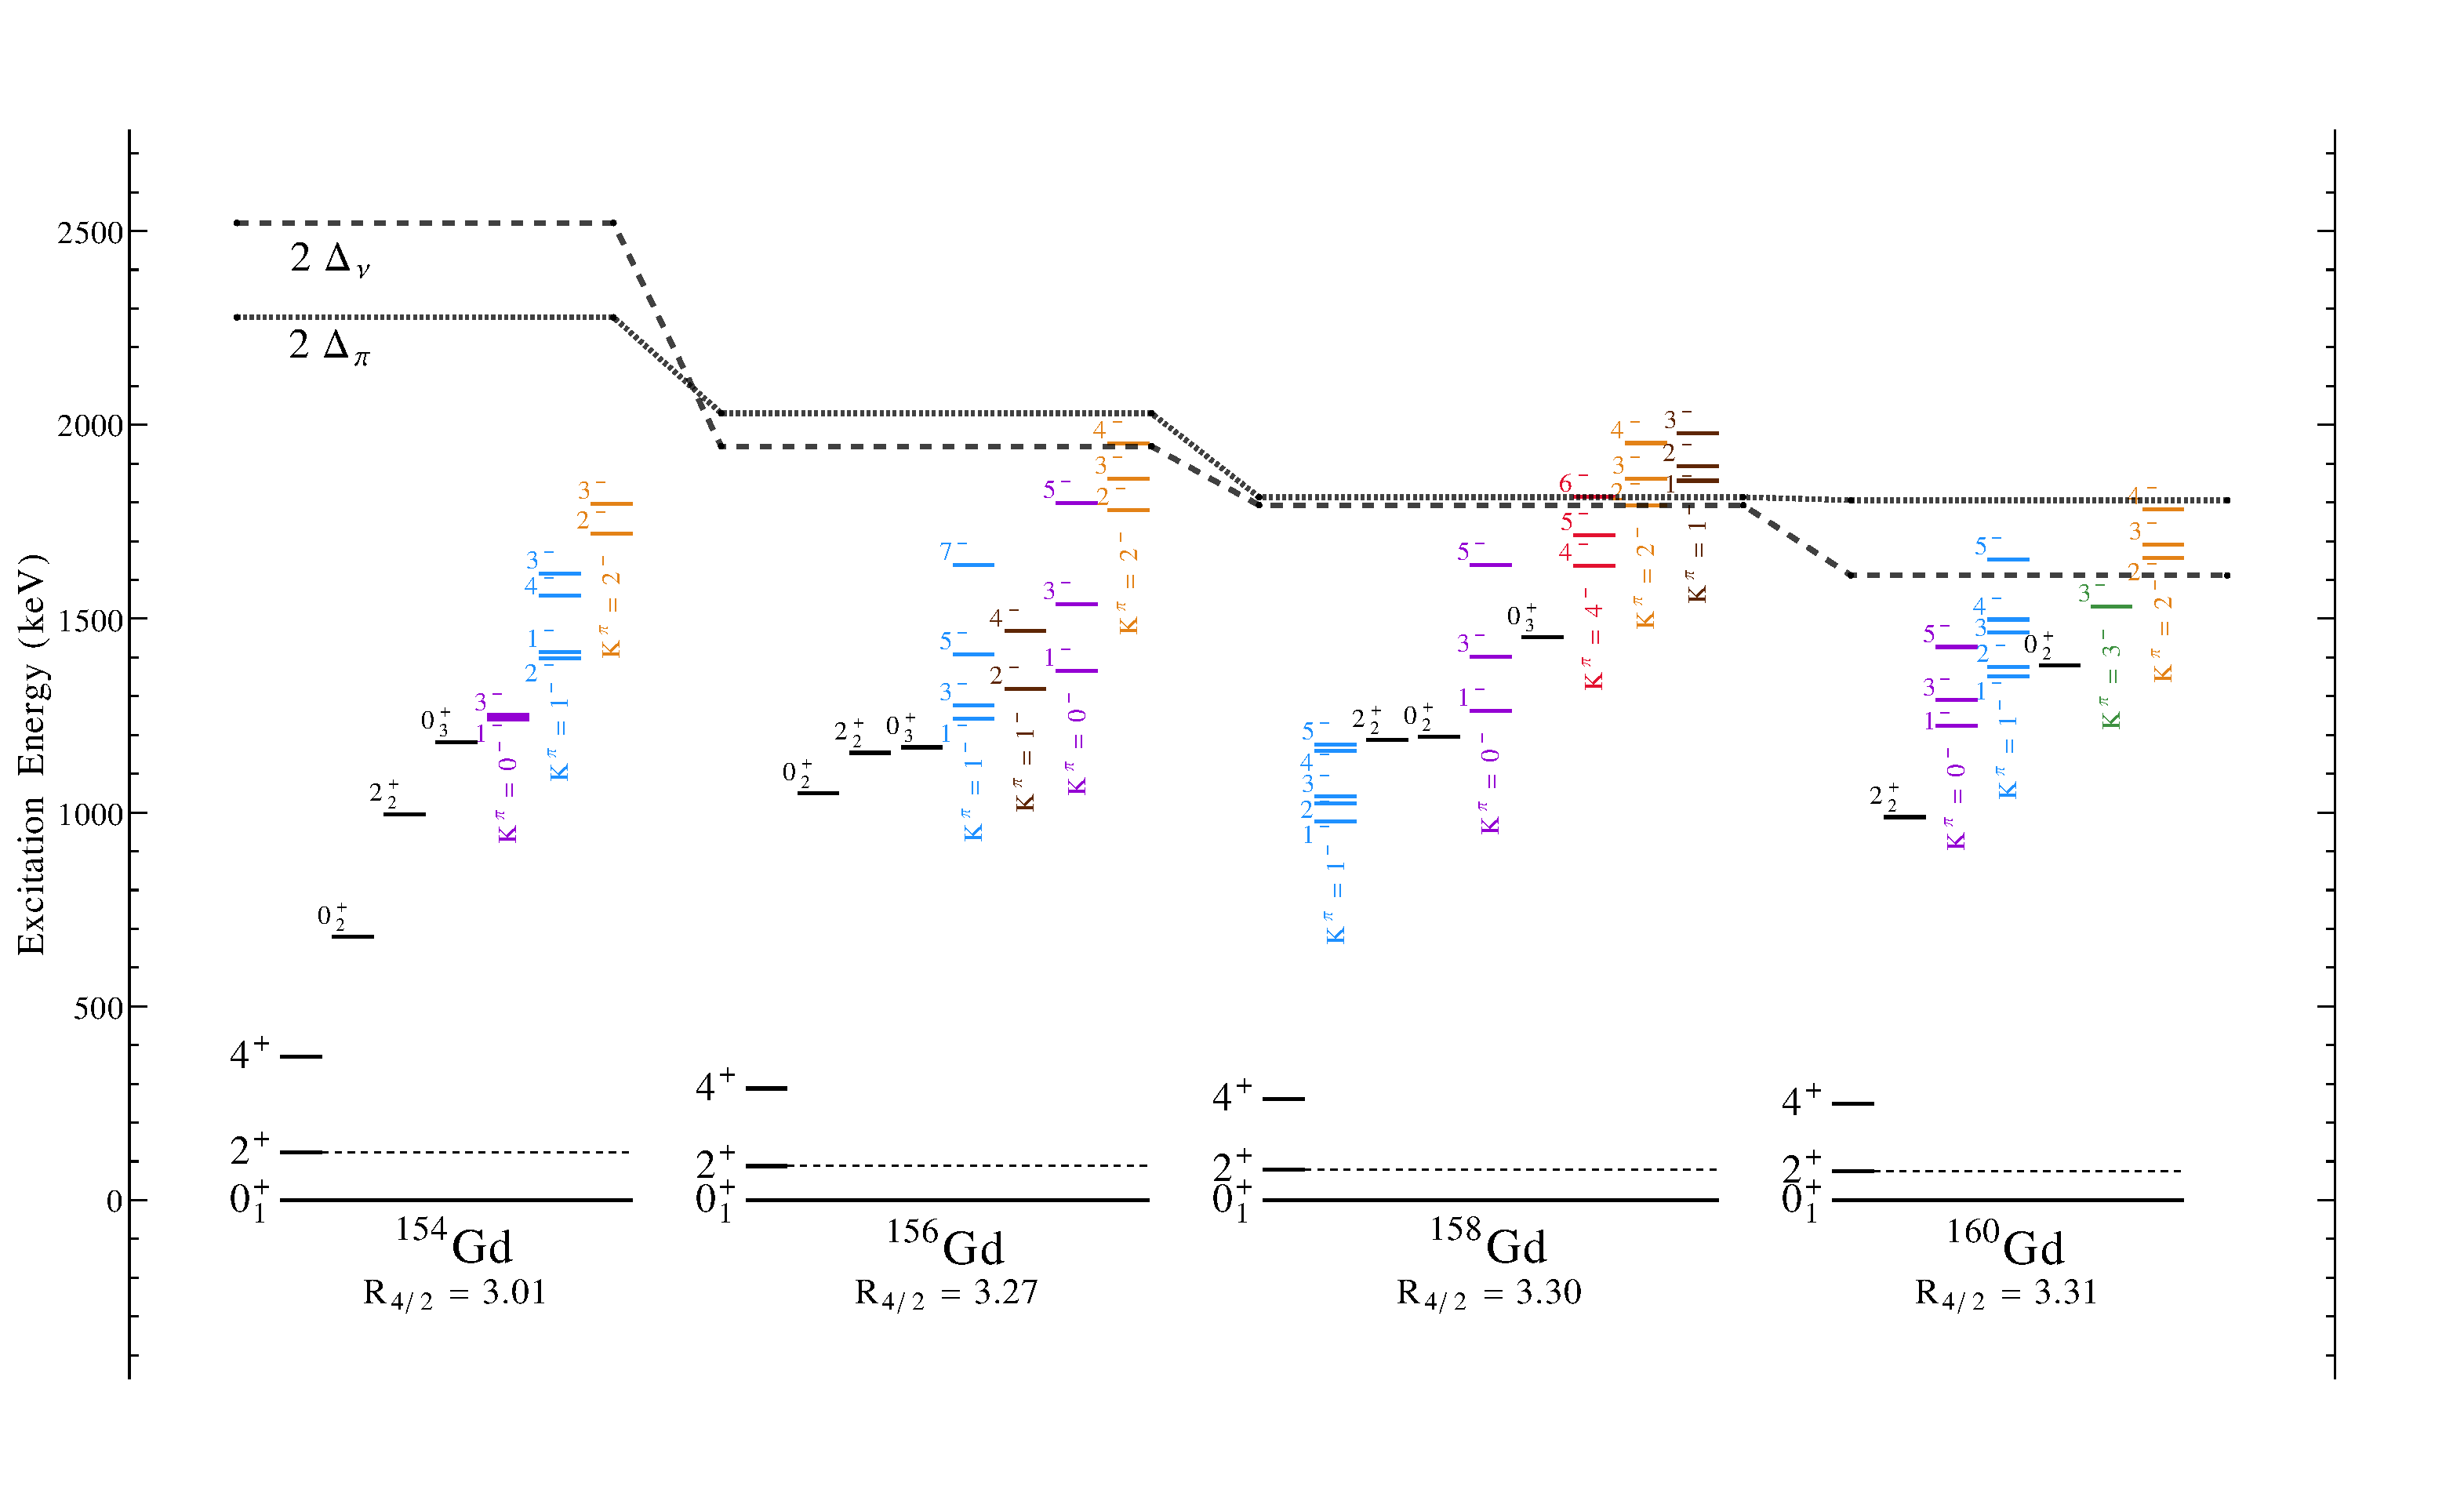
\includegraphics[height=0.8\textheight]{SciDraw_Gd_Octupole_Systematics_FULL.pdf}
\caption{Systematics for the energies of excited negative parity states, the first excited 2$^+$ bandhead, and low-lying excited 0$^+$ states below the pairing gap (2$\Delta_\pi$ and 2$\Delta_\nu$) for even-even Gadolinium nuclei.}
\label{fig:GdSystematics_Octupole}
\end{center}
\end{figure}
\end{landscape}

\begin{landscape}
\begin{figure}[ht] 
\begin{center}
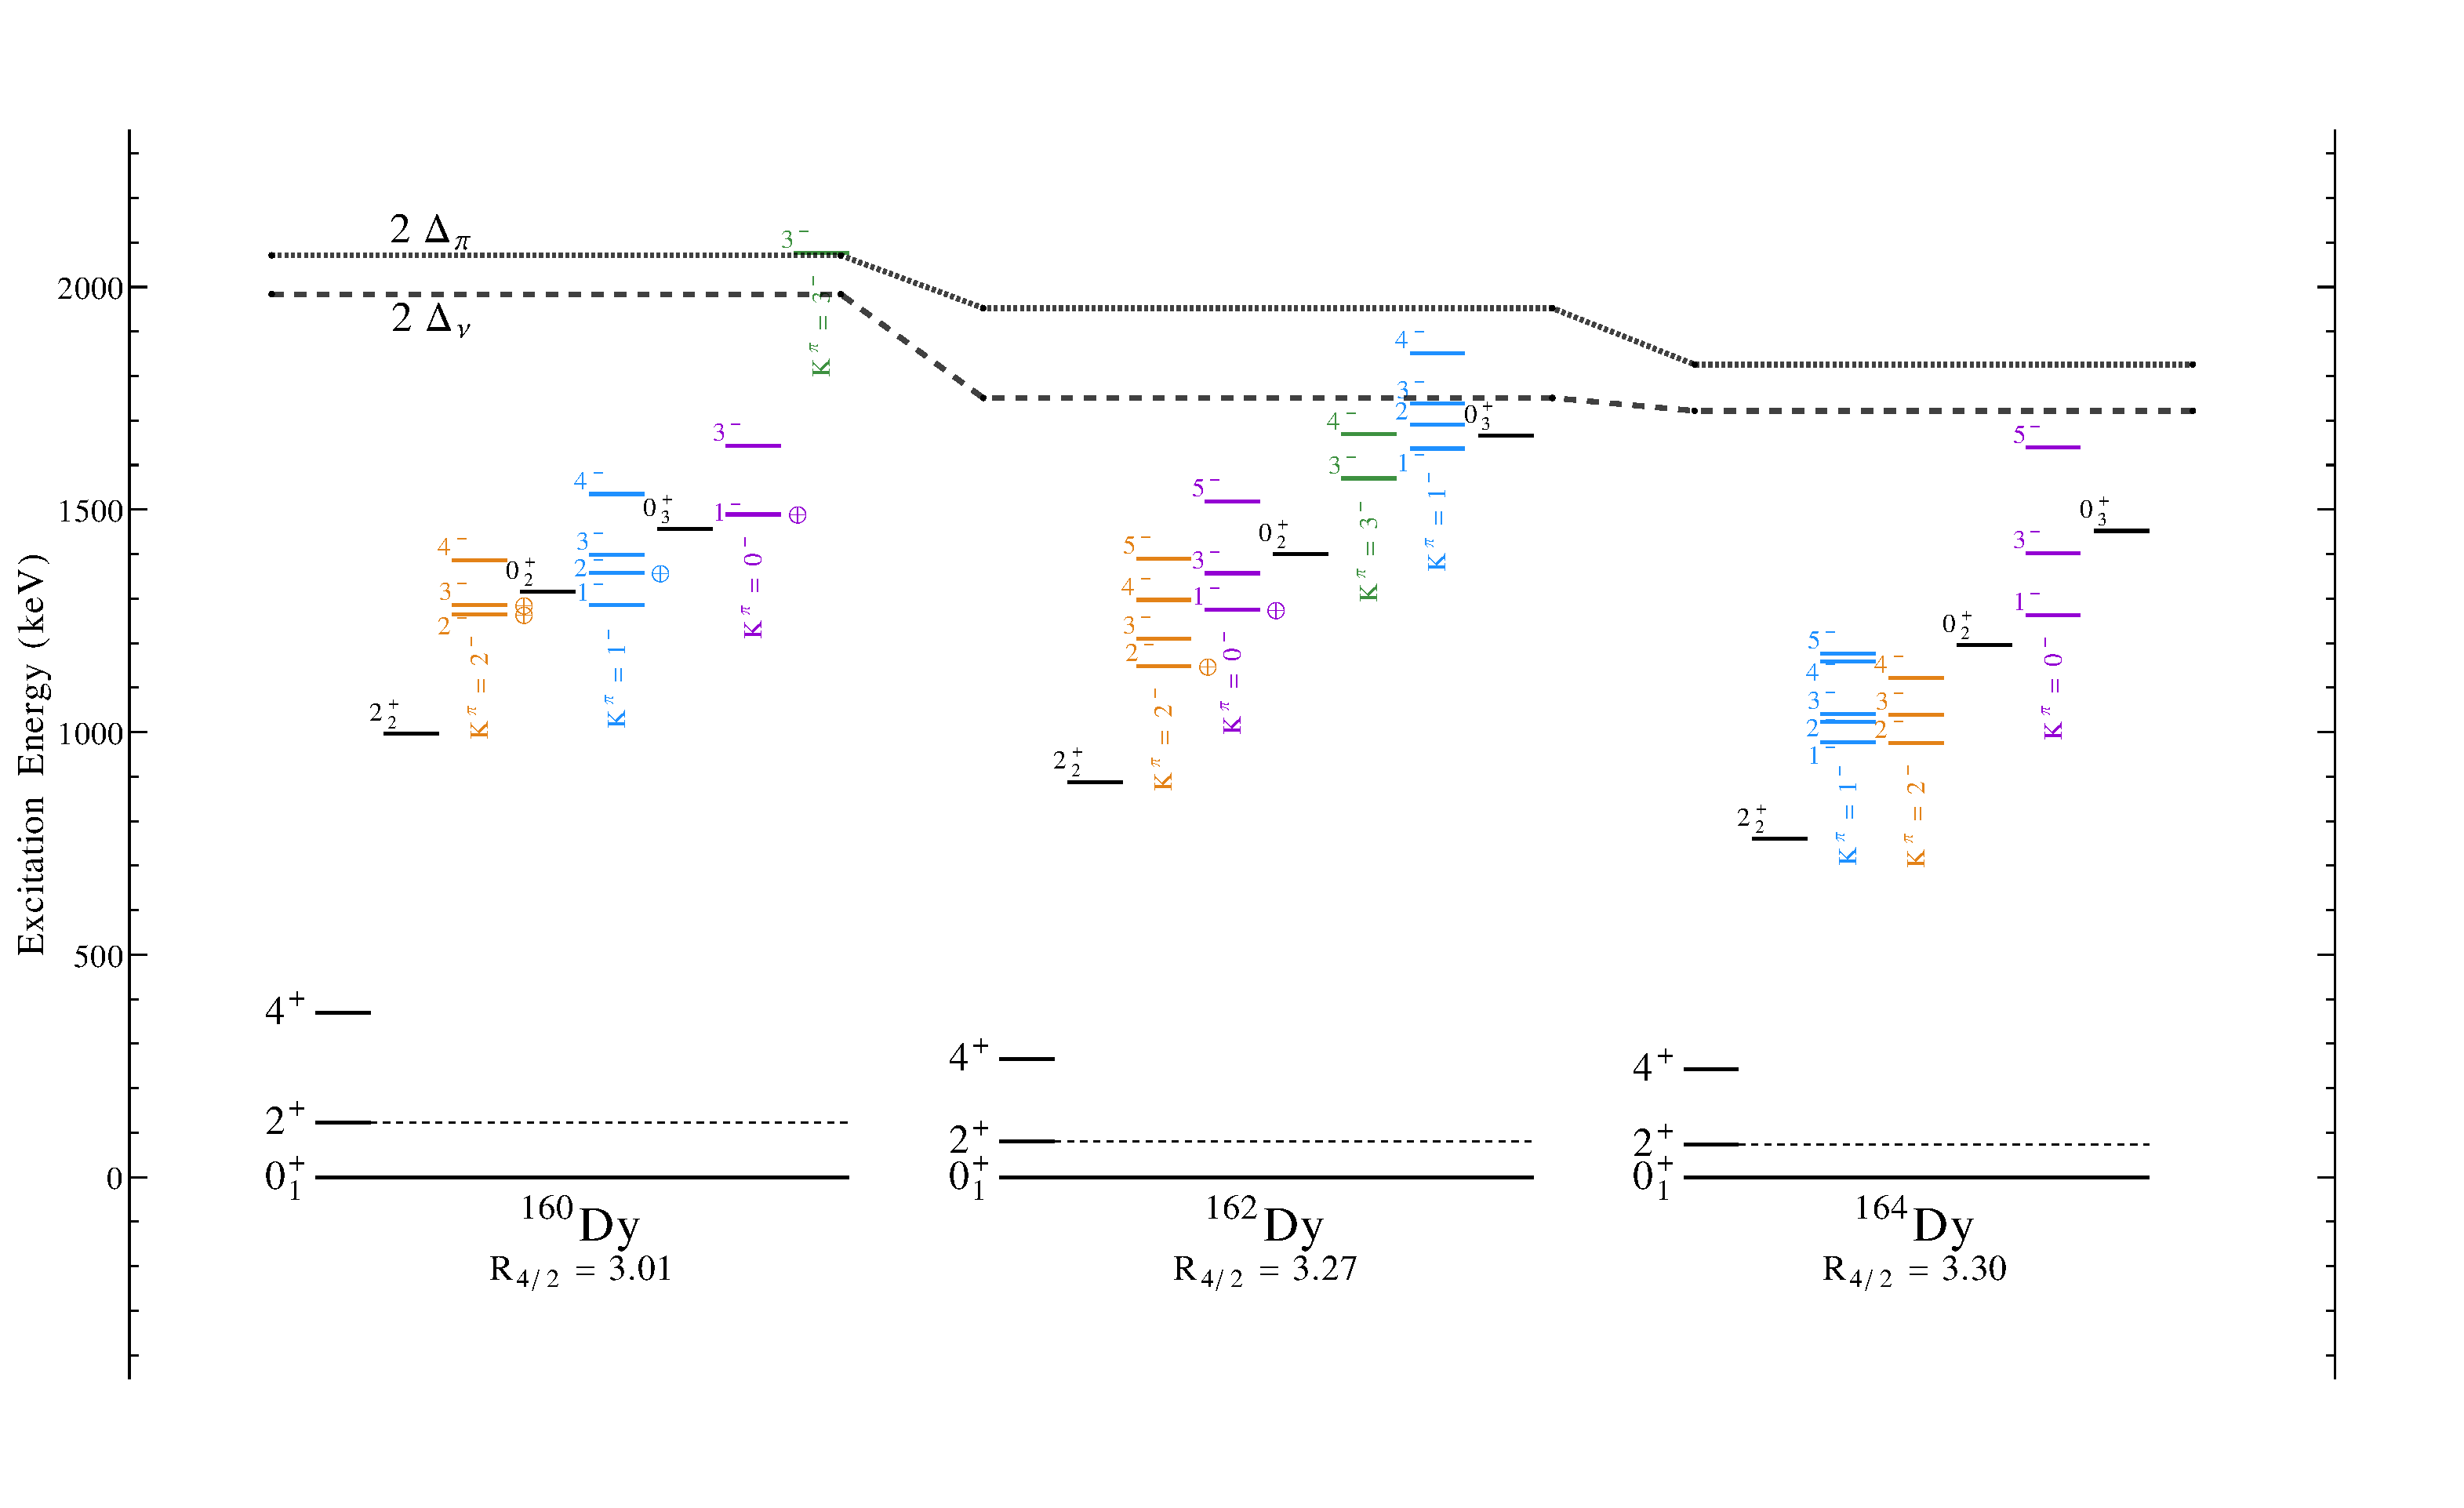
\includegraphics[height=0.8\textheight]{SciDraw_DySystematics_Octupole.pdf}
\caption{Systematics for the energies of excited negative parity states, the first excited 2$^+$ bandhead, and low-lying excited 0$^+$ states below the pairing gap (2$\Delta_\pi$ and 2$\Delta_\nu$) for even-even Dysprosium nuclei. States with a `$\oplus$' marker indicate where a literature lifetime measurement exists.}
\label{fig:DySystematics_Octupole}
\end{center}
\end{figure}
\end{landscape}

\subsection{Multiphonon Configurations in Deformed Nuclei}

We end discussion of the systematics of rare-earth nuclei with any known multiphonon configurations (K$^\pi$=0$^+$,4$^+$ $\gamma\gamma$ type, K$^\pi$=0$^+$ $\beta\beta$). Figure \ref{fig:RareEarth_Multiphonon} contains a series of level schemes of rare-earth nuclei with measured and confirmed two-phonon states; these states are evident by the observation of collective decays to known collective states. For example, the 4$^+$ $\gamma\gamma$-vibration in $^{166}$Er decays via a 7.4~Weisskopf unit B(E2) to the bandhead of the 2$^+$ $\gamma$-vibration (it then subsequently decays via a collective B(E2) to the ground state). As with previous assertions about the `reliability' of the $\gamma$-vibration as a paradigm of nuclear collective vibrations, Figure \ref{fig:Rare_Earth_2g_BE2} shows the absolute  B(E2;2$^+_\gamma\rightarrow$0$^+_{gs}$) measurements in the literature from the K$^\pi$=2$^+$ bandheads, simply to highlight its uniformity over the entire deformed rare-earth region. The trend for Samarium nuclei is drastic, but these isotopes lie in a region of extremely fast shape-change, from nearly spherical to fully deformed within a few nucleons! In a perplexing change of rhetoric in the rare-earths, we observe (and continue to investigate) that many well-deformed nuclei do not exhibit the traditional Bohr-Mottelson behavior of a collective $\beta$-vibration existing as the lowest-lying 0$^+$ state. Instead, many of these lowest-lying 0$^+$ states exist as the $\gamma\gamma$-vibration, with distinctly collective transitions to the 2$^+$ $\gamma$-band. Truly, whether or not the notion of a traditional $\beta$-type vibration is valid seems to be lacking in the deformed case, from the current experimental data. Compare the number of known 0$^+$ $\gamma\gamma$ configurations to the preceeding Figures (\ref{fig:SmSystematics,fig:GdSystematics,fig:DySystematics,fig:ErSystematics,fig:YbSystematics,fig:HfSystematics}) that highlight the status of lifetime measurements of the states and we observe the distinct lack of structure information that still plagues the rare-earth region. No known $\beta\gamma$-vibrations have been observed in the rare-earth nuclei at any excitation energy via a collective transition to a collective $\beta$ or $\gamma$-vibration. However, the 0$^+_5$ state in $^{178}$Hf \textit{could} be the first experimental evidence of a $\beta\beta$ vibration, pending the confirmation of the 0$^+$ state as a collective $\beta$-vibration; as it stands now, the collectivity of the $\beta$-band is tentative, ranging from non-collective to a distinct level of collectivity. If the lowest 0$^+$ band in $^{178}$Hf is indeed a collective $\beta$-vibration, we already have the experimental evidence of a collective transition from another K$^\pi$=0$^+$ band built on top of it, making the 0$^+_5$ band a $\beta\beta$-vibration.

\begin{landscape}
\begin{figure}[ht] 
\begin{center}
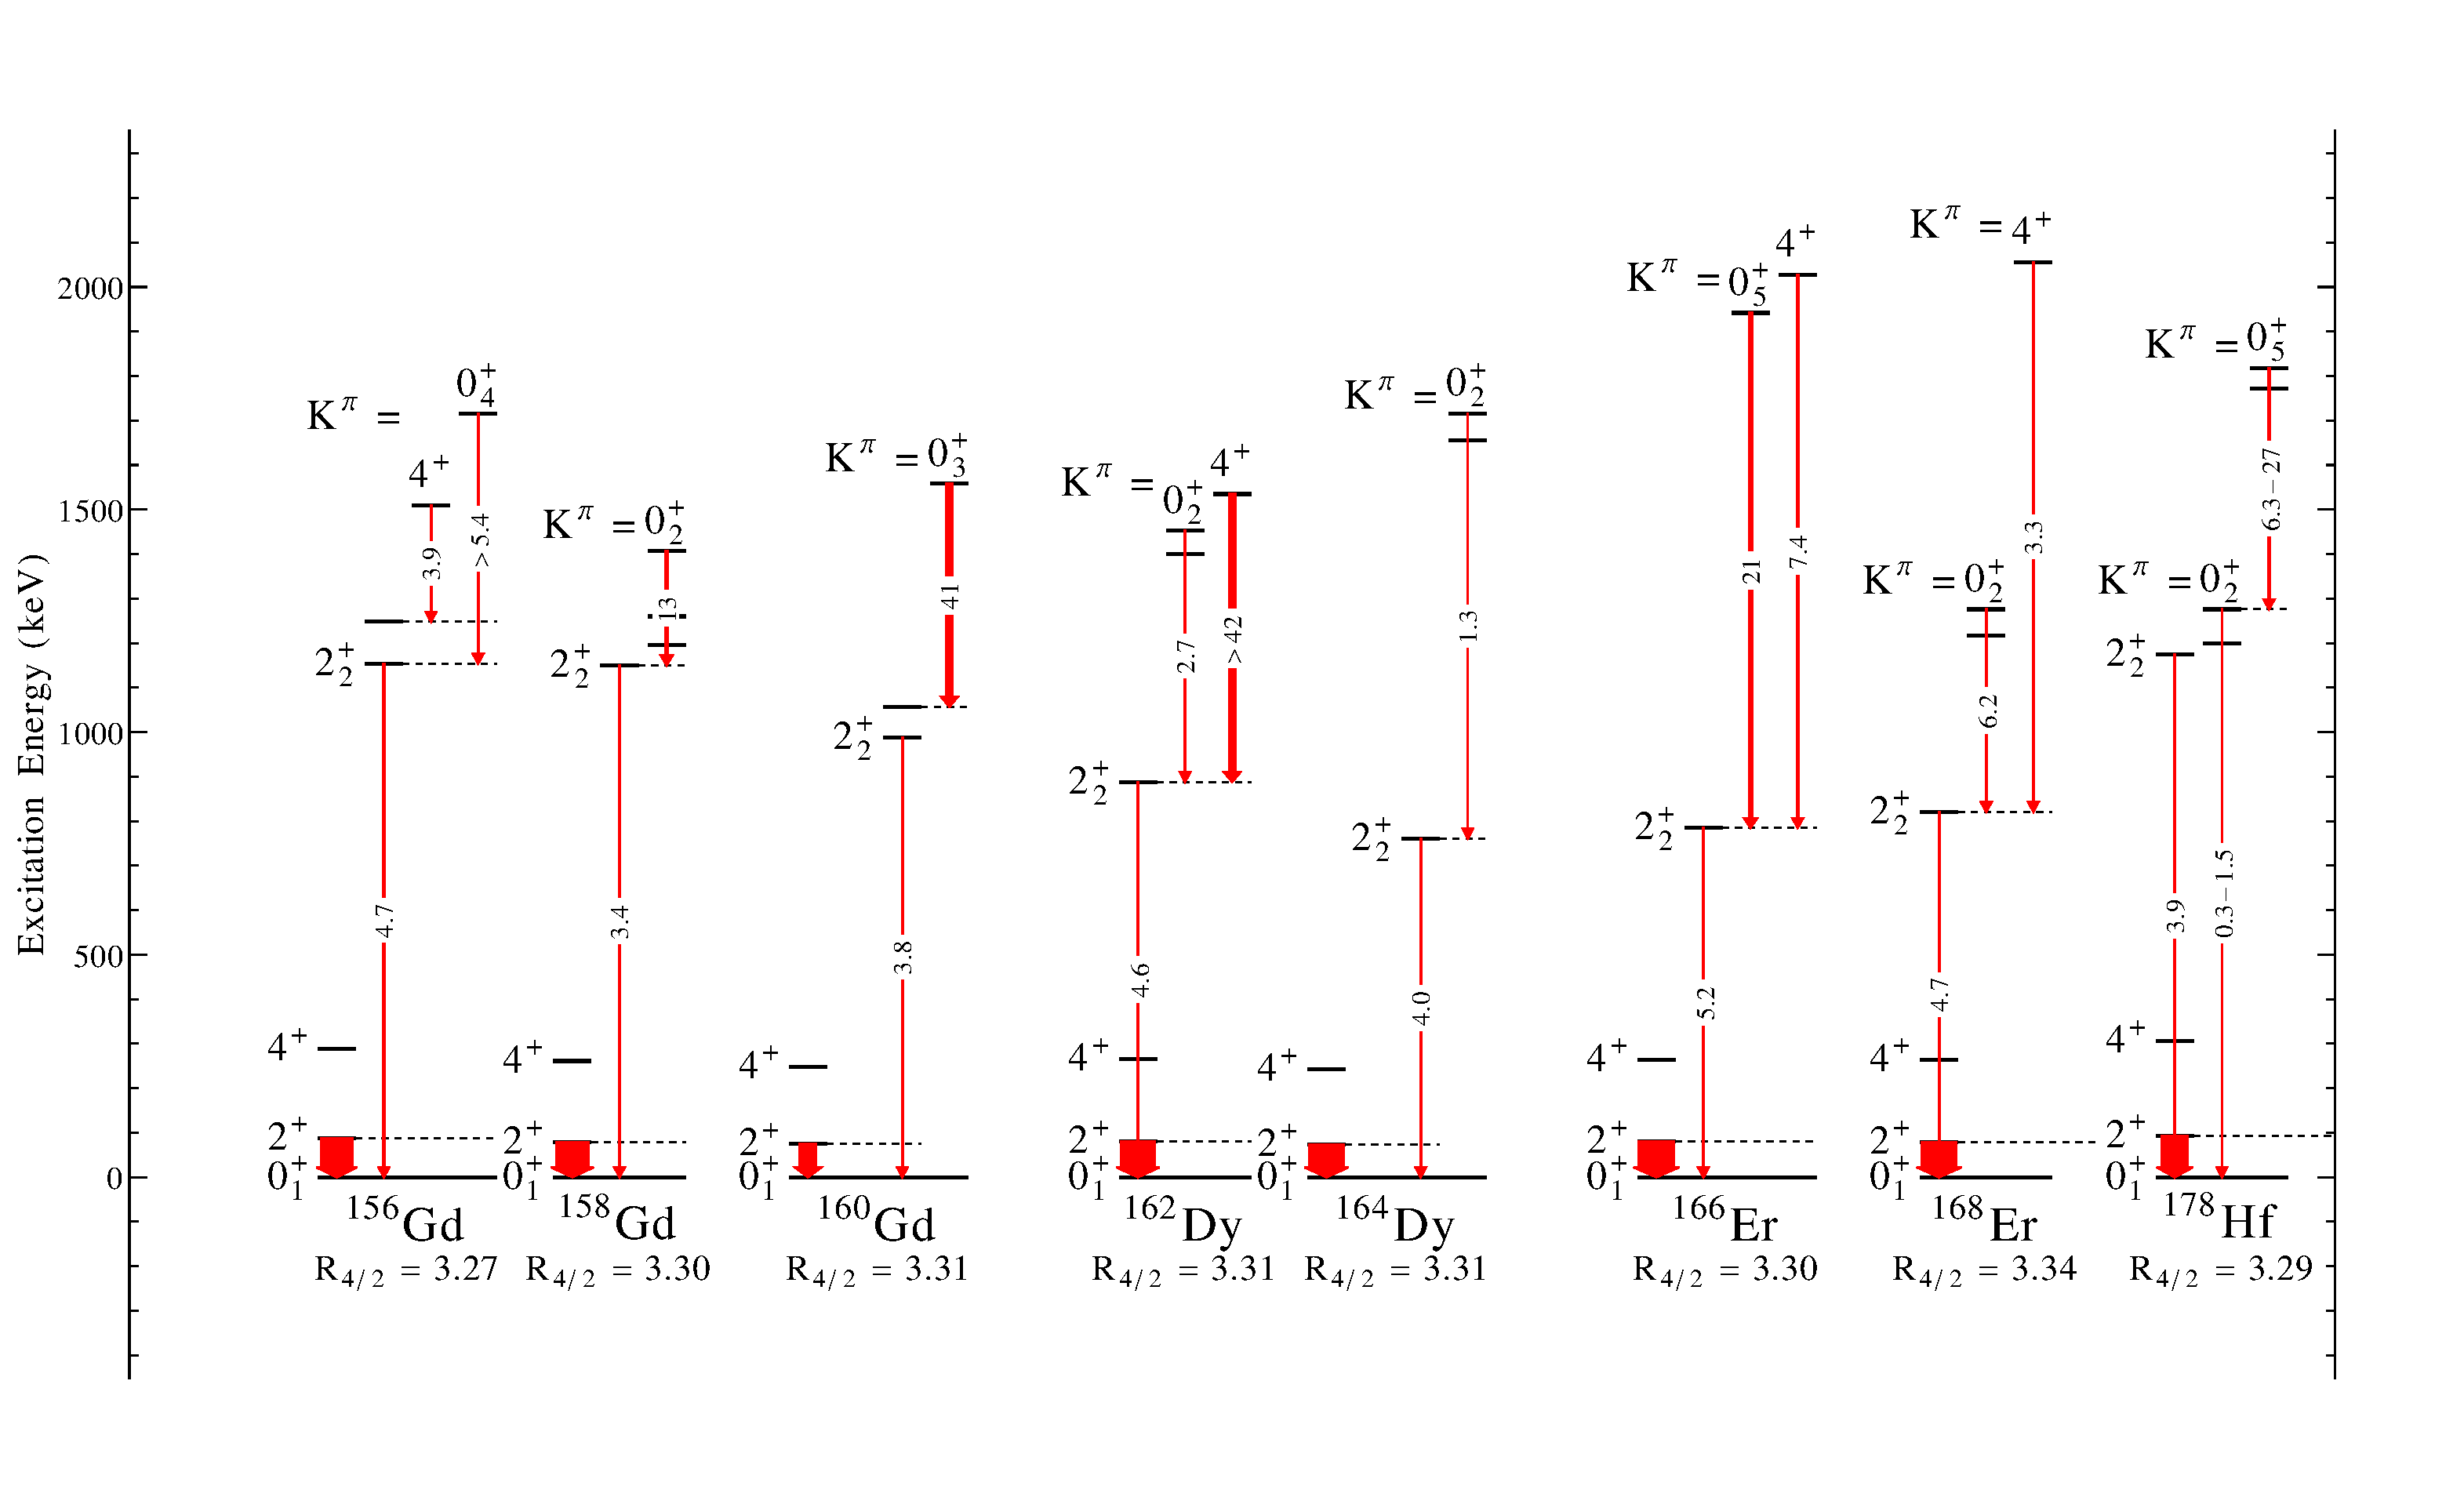
\includegraphics[height=0.8\textheight]{Multiphonon_RareEarths.pdf}
\caption{Summary of all known multiphonon ($\gamma\gamma$, $\beta\gamma$, or $\beta\beta$) configurations in rare-earth nuclei, absolute B(E2) from literature are shown in Weisskopf units to signify collective decays to $\gamma$-vibrational and/or potential $\beta$-vibrational states.
\label{fig:RareEarth_Multiphonon}}
\end{center}
\end{figure}
\end{landscape}

Furthermore, we stress that this problem in nuclear structure is very open, with varied systematic behavior of all K=0 bands in deformed nuclei. In some cases, a collective $\beta$ vibration can be found as the lowest-lying 0$^+$ state, or at a higher excitation energy, in others, the lowest-lying 0$^+$ acts like a collective two-phonon vibration built on top of the $\gamma$-vibration, and in others, one of the higher excitations acts as a $\gamma\gamma$-vibration. Surely, the issue at hand of the nature of 0$^+$ excitations is a wide-open question in nuclear structure, and has been for decades, with a multitude of questions to answer. Can the deformed nucleus act as a near-infinite quantum system with all vibrational degrees available and afforded to it? If we observe well-behaved vibrations in the form of the $\gamma$ bands as the lowest 2$^+$ bands, why do we not have the same B(E2) systematics of the $\beta$-vibration as the lowest 0$^+$ bands? Is the $\beta$ vibration even viable for well-deformed nuclei; if not, what is happening to the $\beta$ vibration across chains of nuclei in the rare-earth region? 


Gadolinium-160 and Dysprosium-162 nuclei both have a very well-deformed shape (R$_\frac{4}{2}$=3.31) as well as a modest number of confirmed and tentative 0$^+$ excitations to study the fasability of vibrational degrees of freedom superimposed on top of a rotational ground state. Literature lifetimes for most states (especially 0$^+$ states and the negative parity states of interest for any octupole correlations) in these nuclei are also scarce, further motivating the lifetime measurements. A great deal of effort and importance is placed on the evolution of nuclear structure across isotopic changes, or at least in a regional scale on the chart of nuclides; the emergence of nuclear data aids in the simultaneous evolution of theoretical efforst to explain the various nuclear structure phenomena at the forefront of nuclear physics. In order to fully ascertain the nature of low-lying excitations (whether they are macroscopic, collective vibrations superimposed on top of a deformed ground state, multiconfigurative particle-quasiparticle states, or something completely different), consistent, precise, and accurate lifetime measurements of excited states must be performed in nuclei where we already have a wealth of spectroscopic knowledge to aid in the characterization of states. 


  %
% Chapter 2
%

\chapter{EXPERIMENTS AND DATA ACQUISITION}

\section{Lifetime Measurements of Excited States}\label{sec:lifetime_measurement_techniques}
The measurement of excited state lifetimes remains an integral part in discerning information about the structure of the nucleus. An abundance of techniques, applicable/sensitive lifetime ranges, and facilities can be implemented to measure these lifetimes in the massive landscape of existing isotopes in nuclei. A schamatic of experimental measures available for use with several lifetime measurement techniques can be found in Figure \ref{fig:VariousLifetimeMeasurements}:

\begin{figure}[h!] 
\begin{center}
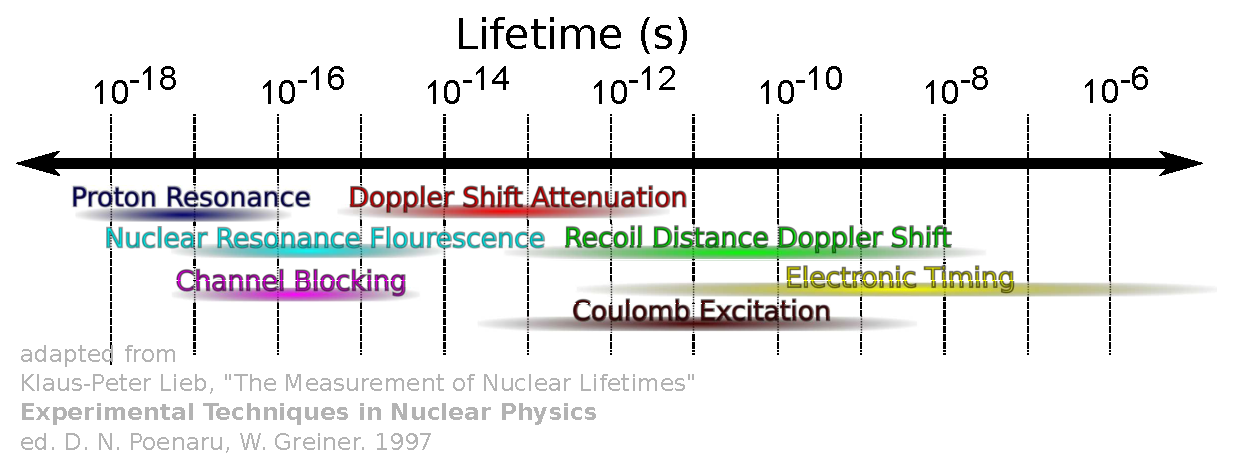
\includegraphics[width=0.95\textwidth]{lifetimes-techniques-full.eps}
\caption{Techniques available to nuclear physicists to measure lifetimes as short as a few attoseconds (10$^{-18}$~s) to the more long-lived lifetimes on the order of microseconds (10$^{-6}$~s) (Adapted from \cite{Poenaru_text}, courtesy of M.~K. Smith).}
\label{fig:VariousLifetimeMeasurements}
\end{center}
\end{figure}

The various lifetime measurement techniques span a tremendous and continuous range of possible lifetimes for nuclear excitations, from $\sim$10$^{-18}$ to $\sim$10$^{-6}$~s, and can be applied to the vast majority of the $\sim$3339 known nuclei in existence (stable and unstable). Several lifetime measurement techniques directly measure the lifetime (or a lifetime-dependent factor in the case of the Doppler Shift Attenuation Method) via various means; techniques like the Recoil Distance Doppler Shift, Coulomb Excitation, and Electronic Timing rely on fast-timing techniques for multiple $\gamma$-ray and/or particle coincidences to measure the lifetimes of metastable states. These direct lifetime measurements apply to the longer-lived excitations (picosecond and above lifetimes), and are contrasted with the more exotic, indirect methods (Proton Resonance, Nuclear Resonance Flourescence, and Channel Blocking) that measure the partial or total Lorentzian energy ($\Gamma\approx\hbar$/$\tau$) width(s) to extract the lifetime of a state. Each lifetime measurements also has its own set of experimental advantages and challenges in addition to their respective sensitive ranges of lifetime measurement. For example, Electronic Timing can measure lifetimes over a very broad range of lifetimes by measuring the time between successive decays into and out of a state, but is limited by the requirement that the particular state desired must be populated via a cascade from higher-lying levels or by charged particle decays. Coulomb excitation offers a relatively simple measurement technique, in that it can directly deduce nuclear lifetimes by measuring the reduced transition probability for direct population of a desired state from the ground state, however, for decays that are not directly linked to the ground state via $\gamma$ decay, this method rapidly increases in complexity. The Recoil Distance Doppler shift method utilizes Doppler-type effects to measure intensities of decay radiation as a function of target position (which then correlates to a nuclear lifetime). This picosecond-range lifetime measurement technique is highly tunable to the precise needs of the experimentalist, yet the methodology and necessary experimental equipment needed can become cumbersome and sophisticated.

Specifically, level lifetimes in the tens to hundreds of femtosecond ($\sim$10$^{-15}$ s) range can be measured with the Doppler Shift Attenuation Method (DSAM), a technique that exploits a recoiling nucleus to produce Doppler shifted $\gamma$-rays when observed at various laboratory angles. The magnitude of the Doppler shift is reliant on a lifetime-dependent factor, which we can easily extract from experiments in the laboratory. DSAM holds a unique place in the overall landscape of lifetime measurement techniques in that it is almost exclusively sensitive in this near-femtosecond timescale. The level lifetimes from DSAM can then be quickly extracted from the angular energy shift(s) of any $\gamma$-rays that de-excite the nucleus.  All of the presented lifetimes in this work are measured with this DSAM technique at the University of Kentucky.

\section{DSAM-INS Formalism}
A $\gamma$-ray observed from a recoiling nucleus will be energy-shifted linearly as a function of the laboratory angle, \textit{$\theta_{lab}$}, shown in Equation \ref{eq:F(tau)}. This angular dependence on the energy is due to observation of Doppler shifted energies of the $\gamma$-ray, based on the detection angle, $\theta_{lab}$, as a $\gamma$ ray observed as the nucleus recoils `away' from the observer will be `red-shifted' down in energy, and inversely (energies will be `blue-shifted') for a $\gamma$ ray observed for nuclei that recoil `towards' the detector.

\begin{equation} \label{eq:F(tau)}
E_{\gamma}(\theta_{lab})=E_{\gamma,o}[1+\beta F(\tau) \cos(\theta_{lab})]
\end{equation}

Here, \textit{E$_{\gamma,o}$} is the unshifted $\gamma$-ray energy, \textit{F}(\textit{$\tau$}) is an attenuation factor, dependent on the lifetime of the excited state (to be discussed in detail in \S \ref{sec:AD_Ft}, as this is one of the key experimental quantities we measure), and $\beta$ is the ratio of the recoil velocity of the target nucleus to the speed of light, \textit{c}; this recoil velocity is derived in Pelte and Schwalm \cite{Pelte_text} from the kinematics involving conservation of momentum and energy in the laboratory frame, and is given by Equation \ref{eq:betarecoil}. 

\begin{equation} \label{eq:betarecoil}
\beta=0.04635 \frac{A_n}{A_n+A_A}\sqrt{\frac{E_n}{A_n}}
\end{equation}

The mass numbers of the bombarding particle and solid target are \textit{A$_n$} and \textit{A$_A$}, respectively, with the bombarding particle energy given by E$_n$ in MeV. In (n,n$^{\prime}\gamma$) experiments, \textit{A$_n$} is unity, while \textit{A$_A$} must take into account the full molecular weight of the target, \textit{e.g.} for Dysprosium-Oxide powder ($^{162}$Dy$_2^{16}$O$_3$), \textit{A$_A$}=162$\times$2+16$\times$3=372. For rare-earth nuclei and \textit{E$_n$}$<$5~MeV, the nuclear recoil velocities are generally less than 1~\% of the speed of light, meaning relativistic effects do not need to be taken into account as they normally would with other lifetime measurement techniques (\textit{e.g.} Recoil Distance Doppler Shift measurements). For example, the recoil velocity $\beta$ for a $^{162}$Dy$_2^{16}$O$_3$ molecule recoiling from a bombarding neutron of 3.1~MeV is 2.1878e-~4. Lifetimes, then, are measured via the single experimental observable, the energy of the $\gamma$ ray as a function of angle; this is achieved at the University of Kentucky with High Purity Germanium detectors with high-resolution $\gamma$-ray spectroscopy to measure precise energy shifts. This excellent energy resolution provided by HPGe detector systems is ideal to measure the $\sim$200-300~eV energy shifts needed, as older fast NaI(Tl) detectors cannot distinguish peaks at such a fine-grain resolution. To highlight this centroid energy shift, Figure \ref{fig:spectra_shift_DSAM} shows a 1902.055~keV $\gamma$-ray Doppler shifting as the detector changes laboratory angle, with the centroids drawn to guide the eye.

\begin{figure}[h] 
\begin{center}
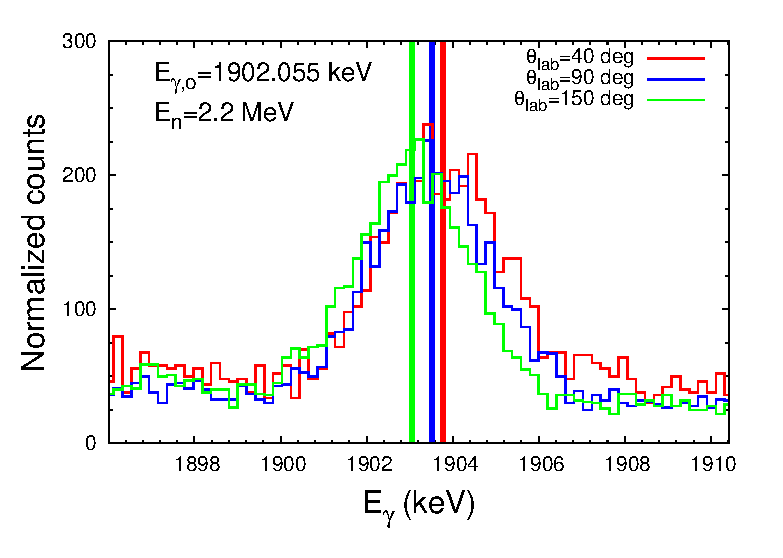
\includegraphics[width=0.97\textwidth]{spectra_shift_DSAM.eps}
\caption{Doppler shift of an E$_\gamma$=1902.055~keV de-excitation from the $\theta_{lab}$=40, 90, and 150 degrees in red, blue, and green, respectively. The vertical lines mark the centroid of each peak of corresponding color.}
\label{fig:spectra_shift_DSAM}
\end{center}
\end{figure}


From Equation \ref{eq:F(tau)}, the only undetermined parameter is \textit{F}(\textit{$\tau$}), an attenuation factor directly dependent on the specific lifetime of the decaying state, formulated by Blaugrund in ref. \cite{BLAUGRUND_DSAM_1966} to be an effect of the recoil nuclei slowing down in the target medium while they decay. \textit{F}(\textit{$\tau$}) can be calculated via multiple formulations, where all formulations rely on an understanding of the nuclear and electronic stopping power of a medium to produce this lifetime dependent attenuation, as the inelastic interaction of the bombarding particle is directly related to these stopping powers. In this work, the Winterbon formalism will be used, where the underlying framework is outlined in \cite{WINTERBON_1975} and \cite{Belgya_DSAM1996}, where an exact solution was obtained for the attenuation factor \textit{F}(\textit{$\tau$}) in terms of the electronic stopping power, the nuclear scattering cross sections, and target density. Key improvements were made to this attenuation factor calculation in the early 1970s by taking the possibility of nuclear deflection during the recoil as well as slowing inside the material lattice into account. This refinement is a necessary addition with the use of large, molar amounts and physical weights of target material, where the electronic stopping power of the medium plays a finite aspect in the calculation of the Winterbon curve; previous (Lindhard and Blaugrand) formulations of the theoretical \textit{F}(\textit{$\tau$}) factors were unable to successfully represent both the nuclear and electronic stopping powers correctly, vastly and systematically underestimating the attenuation. Further advancement of the Winterbon formalism was investigated in \cite{PETERS_DSAM2013}, with attention being placed on the chemical makeup of the target to better characterize the lattice relaxation needed to quantify the nuclear recoil inside the sample. This placed an important focus on the dependence on the oxide powder's consistency and packing density of the molar quantity of the target material inside a container (in our case, a polyethelene vial) when calculating the Winterbon curve.
% [NEED LARGE AMOUNT OF MATERIAL TO PROVIDE STOPPING POWERS (LATTICE NEEDS TO RELAX)]

Note that energy shifts (and thus F($\tau$)) must \textit{always} be positive, in that energies of DSAM $\gamma$ rays are higher at forward angles and lower at backward angles for any realistic system. We will encounter some of the limitations behind measurement of $\gamma$ ray energies via DSAM shortly, and oftentimes, the measured energy shift is either consistent with zero or negative. These limitations in an extraction of F($\tau$) are products of either a lifetime that is outside the range of DSAM, or other factors including sample self-attenuation and/or coincidence with background radiation to blur the centroid energy shift of a particular $\gamma$ ray.

\section{(n,n$^{\prime}\gamma$) Experiments at the University of Kentucky}
DSAM requires the nucleus to be moving as it decays from an excited state for it to be effective, and the preferred probe to excite the nucleus used at the University of Kentucky Accelerator Laboraty (UKAL) is the inelastic scattering of neutrons. The inelastic scattering reaction imparts some velocity to the target nuclei, fulfilling the base requisite for DSAM, that the target is moving as it decays. In years past, thermal neutrons from various fission sources have been utilized to perform the inelastic scattering reactions, but the accessibility of monoenergetic neutrons has made UKAL a popular and unique setting in the realm of experimental structure physics. Energetic neutrons cannot be accelerated with a standard electrostatic accelerator due to their neutral charge-state, so non-thermalized neutrons must be produced via a primary reaction. This mechanism is outlined in Equation \ref{eq:3HQvalue}.
\begin{equation} \label{eq:3HQvalue}
\text{${}^3$H(p,n)${}^3$He, Q = -0.763 MeV}
\end{equation}

This $^3$H(p,n) reaction produces quasi-monoenergetic neutrons, tunable to a desired energy in a 0.5~-~5.5~MeV bombarding neutron energy range, ideal for studying the low-lying states in nuclei. UKAL uses their on-site 7~MV single-ended Van DeGraff accelerator to accelerate a bunched, pulsed beam (at a frequency of 1.875~MHz) of protons to impinge on a pressurized (slightly above atmospheric at $\sim$110 kPa) tritium gas cell, prompting the reaction to produce a forward cone of neutrons. A slight energy spread is present in the outgoing neutrons due to a thin molybdenum foil to prevent the gas cell from out-gassing upstream, which would catastropically contaminate the entire beamline with radioactive $^3$H. This energy straggling is minute, however, providing a $\sim$2.5\% energy spread on average at 50-100~keV standard deviation on neutron energy \cite{Belgya_DSAM1996}. %A forward-monitor measurement of this neutron energy spread is shown in [FIGURE HERE AND ASK SHELLY ABOUT FWD MONITOR] and is typically on the order of $\sim$50~keV. 

The choice of neutrons as a probe can be justified for multiple reasons, and brings its set of distinct advantages; the inelastic scattering and low-spin transfer leaves the nucleus in excited, aligned states with relatively low angular momentum. Generally, spin 5$^{\pm}$ states are the practical limit of angular momentum that can be imparted in an inelastic scattering reaction with neutrons at the University of Kentucky. This low-spin population of states is because the spin-1/2 neutron would naturally not be able to produce a higher spin state without the addition of a very large amount of angular momentum during the inelastic scattering reaction. The neutral charge of the neutron also implies that the scattering reaction is not impeded by the Coulomb barrier; this means that levels are populated very close to the bombarding neutron energy. Lastly, the excited states populated by inelastic neutron scattering are generally nonselective, in that either single-particle excitations or collective states can be populated, allowing the study of both types of excitation. The Doppler Shift method also offers the unique ability to tune bombarding neutron energies to populate states at or very near their threshold energies. This effect is two-fold: first, the experimentally determined F($\tau$) factor from Equation \ref{eq:F(tau)} is directly dependent on the incoming neutron energy, so minimization of the neutron energy is key to extraction of the lifetime, so the `observed' F($\tau$) will be inflated for higher neutron energies. Secondly, this `dialing-in' of neutron energy can completely remove any lifetime inflation due to feeding from higher-lying states; DSAM is unique in this aspect because the other methods of measuring a nuclear lifetime will be unable to remove this feeding, or in some cases (such as the Gamma Ray Induced Doppler Broadening technique), the feeding will manifest as a large uncertainty in measurement.

DSAM following inelastic neutron scattering is not without its downsides or experimental challenges to overcome. Since the target has significant thickness and involves molar quantities of target powder, $\gamma$ rays from deep inside the sample will be attenuated in their trajectory out of the sample. This has a two-fold effect, in that the absolute intensity must be corrected for (explained in detail in \S \ref{sec:gambit_correction}) low-energy $\gamma$ rays that could easily become fully attenuated and absorbed by the target material, and that any lifetimes extracted from the linear shift of energy \textit{may} not be trustworthy, as the energy attenuation is strongly angular dependent, effectively `flattening' the Doppler energy shift. 

The ensemble of (n,n$^\prime\gamma$) experiments performed at UKAL can be achieved with the relatively simple experimental setup, shown in Figure \ref{fig:ExpSetup}.

\begin{figure}[h!] 
\begin{center}
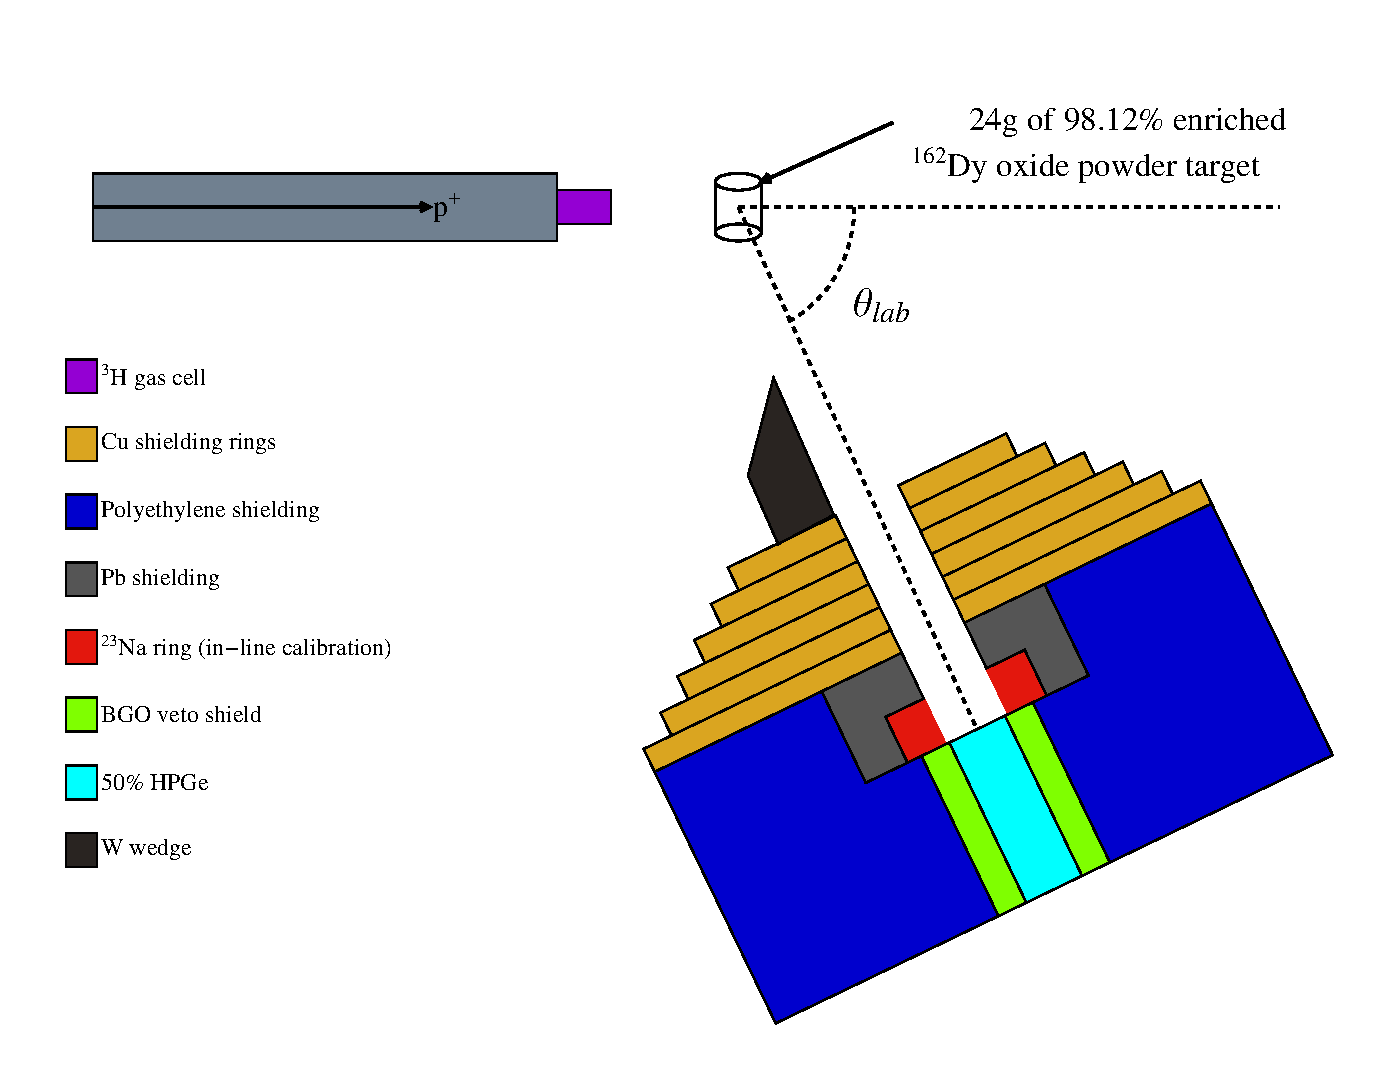
\includegraphics[width=0.97\textwidth]{SciDraw_ExpSetup_Dy.eps}
\caption{Sample Experimental Setup at UKAL for $\gamma$-singles measurements (Made in M. Caprio's SciDraw software for Mathematica \cite{Caprio2005107})}
\label{fig:ExpSetup}
\end{center}
\end{figure}

The single 50\% relative efficiency Ortec HPGe planar detector (named after the 1904 Kentucky Derby winner Elwood) sits $\sim$125~cm away from the end of the beamline on a goniometer equipped circular track $\sim$2~m in radius to observe $\gamma$-rays at various laboratory angles. In Figure \ref{fig:ExpSetup}, the target (a cylindrical polyethelene vial of enriched target powder) is suspended a few ($\sim$4) inches away from the end of the tritium gas cell, where monoenergetic neutrons will inelastically scatter off the target, prompting $\gamma$ decay from the sample to be observed by the HPGe detector. The proximity of the target in relation to the end of the tritium gas cell ensures that the highest possible neutron flux from the forward cone of neutrons will strike the majority of the target material. The castle of passive shielding materials are two-fold in use: to lower background radiation in spectra and to diminish fast neutron damage to the HPGe detector itself. The viewing channel of the detector is lined with copper plating to absorb fast neutrons from the tritium gas cell at the end of the beamline. In addition, borated polyethelene surrounds the detector to reduce secondary \& tertiary scattering of neutrons and $\gamma$-rays from reaching the detector; the typical ensemble of lead rings also aid in regular $\gamma$ background reduction. Lastly, a wedge of tungsten is placed in direct view of the tritium gas cell to act as a shadow bar to prevent neutrons from directly entering the detector from the gas cell. An ensemble of BGO (Bismuth Germanate Oxide) scintillators are placed annularly around the HPGe detector to further aid in Compton scattering background suppression; these scintillation detectors provide an anti-coincidence to veto background events that occur, actively cleaning spectra.

Spectra are generated from the Time of Flight (TOF) technique to discriminate background events from prompt $\gamma$ events; a time-to-amplitude converter (TAC) measures the relative time between events in the HPGe detector and a beam pick-off signal near the end of the beamline. At UKAL, the events in the HPGe act as the `start' and the pick-off serves as the `stop' as to not flood the electronics from pick-off signals that do not result in detected radiation. The concept of the TOF technique is that particles and $\gamma$-rays require different amounts of time to reach a detector, dependent on their velocity (neutrons of a velocity $\ll$ \textit{c} take longer to reach a detector than a $\gamma$-ray traveling at the speed of light). This time difference between measured events is recorded by the TAC, and TOF spectra are generated through a built-in single channel analyzer (SCA). Specifically at UKAL though, the neutron events occur \textit{first} as they scatter off the various materials (mainly primary scattering off iron) in between the target and detector face, while the speed of light $\gamma$-ray events occur in the larger peak. The resultant spectrum is used to properly gate the experimental datasets in the analog-to-digital converter (ADC) by only selecting corresponding prompt $\gamma$-ray events from the histogram. An example of a typical TOF spectrum from experiments at UKAL is shown in Figure \ref{fig:TOF_spec}.

\begin{figure}[h] 
\begin{center}
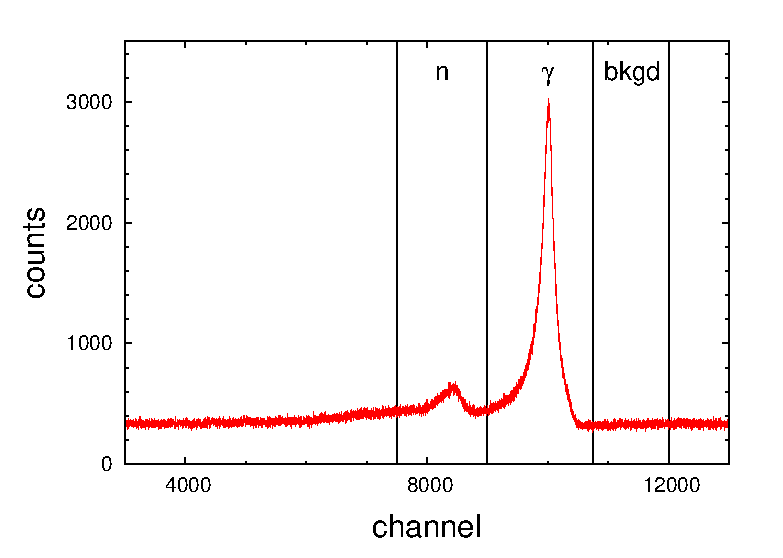
\includegraphics[width=0.97\textwidth]{TAC_spectrum.eps}
\caption{Typical TOF spectrum with labeled regions for corresponding $\gamma$, neutron, and background events.\label{fig:TOF_spec}} %Note the passage of time to the left, starting at the prompt $\gamma$-ray peak, followed by a neutron bump, and wrapping back around the x-axis.
\end{center}
\end{figure}

The single-detector setup and $\gamma$-singles based experiments provide more distinct downsides to lifetime measurements via DSAM at the University of Kentucky in particular. The limitations of not using $\gamma$-$\gamma$ coincidences can have profound implications on the visibility and overall statistics of spectra gathered from the experiment(s); being able to apply timing gates on individual $\gamma$-decays is an extremely powerful tool in determining decay patterns, cascades, and lower-intensity peaks for interband decays. One detector setups require a considerable length to the experimental campaign, and is a severe limitation to the facilities, where the experimenters must enter the target room periodically throughout the run to physically move the detector across the entire range of angles used in the measurements, and must systematically scan through the entire range one angle at a time. Given an unlimited amount of beamtime with little to no deadlines, this is not a problem, however, a modest amount of statistics for $\gamma$-decays observed in a typical measurement require up to (in some cases in excess) a week of continuous beamtime for a single neutron energy angular distribution. 
% Background-subtracted spectra are then generated by subtracting any events that correspond to the random background region from the prompt $\gamma$-ray gated events from the TAC spectrum in Figure \ref{fig:TOF_spec}.

\subsection{Excitation Function Measurements}
Typically, the first measurements to be made are excitation function measurements; these supplement the $\gamma$-singles nature of the angular distribution measurements, to help infer the ideal bombarding neutron energy for peak $\gamma$-ray population rates. In stark contrast to the angular distributions where the neutron energy is kept constant, the excitation functions modulate the bombarding neutron energy to provide the $\gamma$-ray population strengths as a function of neutron energy. Similarly in contrast, the HPGe detector is kept at a constant laboratory angle of 90 degrees with respect to the beamline. An extremely powerful tool, these excitation functions provide important insight into the nature of any observed $\gamma$-rays; for a particular excited state that de-excites via multiple channels, the corresponding $\gamma$-rays will have both the same a) quantitative threshold, and b) qualitative shape. The absolute threshold allows previously unidentified or unplaced $\gamma$-ray transitions to be placed into a known level scheme, as the threshold for the de-excitation must match the level energy. If the populated level's spin are high (5$^\pm$), the threshold will be higher than the level energy, as the bombarding neutron must have higher linear momentum (energy) to successfully provide enough angular momentum transfer during the reaction. The qualitative shape of the excitation functions is heavily dependent on the initial spin and parity of the de-exciting level, making $\gamma$-ray discrimination and identification from different levels a trivial task. This identical shape also allows the relative intensities of $\gamma$-rays to be inferred (independent of the absolute intensities we can gather from the angular distribution measurements), since we can take the ratio of matched-shape excitation functions. An example of two matching $\gamma$-ray transitions from the same level (J$^\pi$=5$^-$), contrasted with a $\gamma$-ray from another level (J$^\pi$=1$^-$) is shown in Figure \ref{fig:matching_exf}. 

\begin{figure}[h] 
\begin{center}
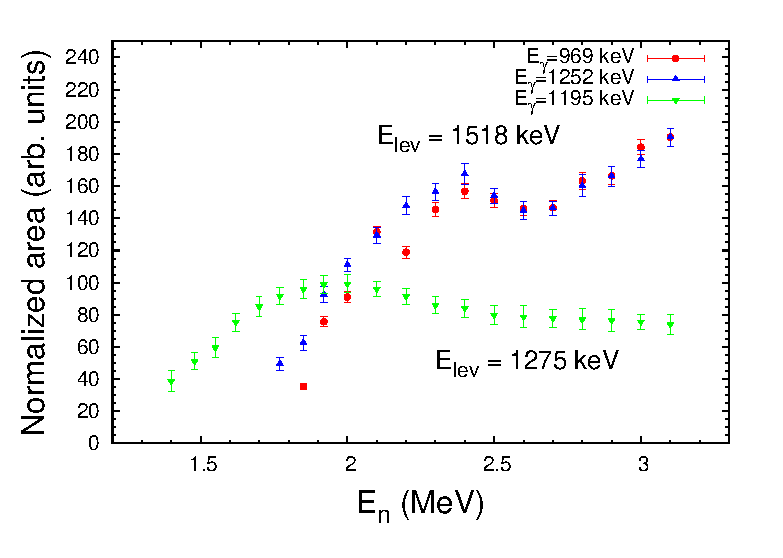
\includegraphics[width=0.97\textwidth]{matching_exf.eps}
\caption{Superimposed excitation functions for two gamma rays (E$_\gamma$=969 \& 1252~keV) leaving the same level (E$_{lev}$=1518~keV), and a single 1195~keV $\gamma$-ray leaving a separate E$_{lev}$=1275~keV level in $^{162}$Dy. The different thresholds and shape of the 1195~keV and 969~keV de-excitations imply that these decays are from two different levels, clearly showing their placement in the level scheme.}
\label{fig:matching_exf}
\end{center}
\end{figure}

The excitation function measurements serve as a quasi-replacement for $\gamma$-$\gamma$ coincidences in a particular experiment, as it allows retention of good statistics that one would get from $\gamma$-singles spectroscopy. With $\gamma$-$\gamma$ coincidences, a level scheme can be built extremely easily, because coincident $\gamma$-decay chains into and out of levels are unquestionably vivid in multiple HPGe detectors; this is not the case in a $\gamma$-singles experiment, since a) particular $\gamma$-rays appear only in the single HPGe detector, and b) discrimination of decay chains is impossible with $\gamma$-singles. The excitation function allows a level scheme to be built in a similar fashion to $\gamma$-$\gamma$ coincidences, while only requiring a single detector, because threshold energies are obvious, and that the qualitative shape of the excitation functions will be identical. Without either implemented technique (excitation function measurements or $\gamma$-$\gamma$ coincidences), proper $\gamma$-spectroscopy would be rendered impossible, as we would no longer be able to confidently place $\gamma$ decays to levels or assign level lifetimes from the Doppler Shift Attenuation measurements.
%[EXPAND ON THIS, CAN BUILD LEVEL SCHEME IN SIMILAR WAYS, ETC].
\subsection{Angular Distribution Measurements}
To extract the lifetimes of excited states, the angular distribution of gamma rays must be measured, specifically, the energy dependence of $\gamma$ rays as a function of lab angle; this is achieved at UKAL with the same single High-Purity Germanium detector used in the excitation function measurements. By physically moving the HPGe detector to different laboratory angles on the circular track, we can extract multiple observable quantities from the angular distribution measurements. First, \textit{F}(\textit{$\tau$}) is found by plotting \textit{E$_{\gamma}$} as a function of cos($\theta$); the relation in Equation \ref{eq:F(tau)} states that the centroid energy shift of a $\gamma$-ray will be linear with cosine, with \textit{F}(\textit{$\tau$}) being the slope. Comparison of this experimental \textit{F}(\textit{$\tau$}) factor with the theoretical calculation for \textit{F}(\textit{$\tau$}) allows extraction of a lifetime \textit{$\tau$} for the decay radiation and excited state. Special care must be taken when measuring the lifetimes, because higher-lying levels can introduce feeding transitions into lower-lying states, inflating the measured lifetimes. Since the theoretical \textit{F}(\textit{$\tau$}) factor is directly dependent on the recoil velocity (the bombarding neutron energy), additional inflation will also be introduced when extracting lifetimes for levels far below the bombarding neutron energy. Performing the excitation function measurements first allows for the minimization of lifetime inflation while maximizing population rate for a particular excited state, as we know the approximate population as a function of bombarding neutron energy.   

When the nucleus decays from an aligned state, the classical radiation pattern of the $\gamma$-ray can be expressed by the sum of even Legendre polynomials as a function of $\cos(\theta)$ (Equation \ref{eq:angdistW}), where the coefficients for each order polynomial are directly related to the multipolarity of the transition. Realistically, only the coefficients a$_2$ and a$_4$ are considered, since the higher order terms correspond to the contributions from the insignificantly intense multipolarities for $\Delta$J$>$2.
%SHOW DERIVATION FIGURE HERE

\begin{equation} \label{eq:angdistW}
W(\theta)=\sum_{\text{even k}}\alpha_k\text{P}_k\cos(\theta) \Rightarrow W(\theta) \approx \text{A}_0[1+\text{a}_2\text{P}_2\cos(\theta)+\text{a}_4\text{P}_4\cos(\theta)]
\end{equation}

The anisotropic nature of the $\gamma$ radiation produced arises from the fact that parity conserving nuclear reactions, \textit{e.g.} (n,n$^{\prime}\gamma$), and a defined beam direction, create a plane of interaction . Otherwise, the random orientation of nuclei in space would mean all multipolarities of $\gamma$ radiation  have isotropic angular distributions. By comparing the relative magnitude and sign of the a$_2$ and a$_4$ coefficients, limits can be placed on both the spin and parity of the de-exciting level, because dipole and quadrupole radiation patterns have distinct shapes (shown in Figure \ref{fig:multipole_diff}). These same Legendre Polynomial coefficients can also be compared to theoretical calculations to extract multipole mixing fractions ($\delta$) for mixed-multipolarity transitions. This multipole mixing fraction is simply the ratio of E2 transition strength to M1 transition strength:

\begin{equation} \label{eq:multipolemixing}
\delta=\frac{\langle\eta\vert E2 \vert\nu\rangle}{\langle\eta\vert M1 \vert\nu\rangle}
\end{equation}

\begin{figure}[h] 
\begin{center}
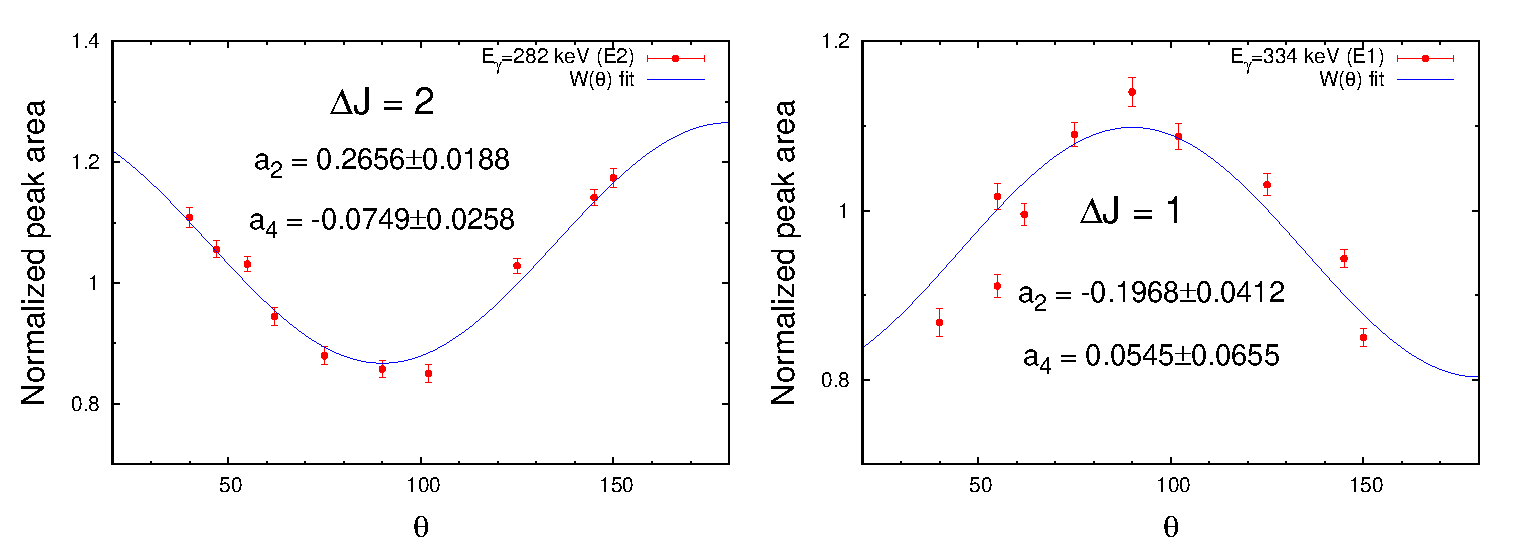
\includegraphics[width=0.97\textwidth]{multipole_diff.eps}
\caption{Angular distributions for two different multipolarity $\gamma$-rays in $^{162}$Dy, an E2 transition of E$_\gamma$=282~keV (the 6$^+_{gs}\rightarrow$4$^+_{gs}$ transition) \& an E1 transition of E$_\gamma$=334~keV (a 3$^-\rightarrow$2$^+_\gamma$ transition), showing distinct, inverted shapes.}
\label{fig:multipole_diff}
\end{center}
\end{figure}

Lastly, the angular distributions allow us to measure the absolute intensity of emitted $\gamma$-rays from the A$_0$ coefficient. In experiments with static, symmetric detectors (\textit{e.g.} two detectors at 90$^{\circ}$), only the relative intensity of $\gamma$ rays can be extracted. Though seemingly simple in form and funciton, the $\gamma$-singles measurements made at UKAL are an incredibly powerful tool that yield a wealth of knowledge about the structure of the nucleus.

\section{Experimental Campaigns}
Two sets of experimental campaigns were performed at the University of Kentucky to measure the level lifetimes for deformed rare-earth nuclei, $^{160}$Gd and $^{162}$Dy. Both targets were acquired from Oak Ridge National Laboratory in the form of an isotopically enriched oxide powder (specifically, $^{160}$Gd$_2^{16}$O$_3$ \& $^{162}$Dy$_2^{16}$O$_3$); the sample powder was then placed into a 1.5$^{\prime\prime}$ diameter by 3$^{\prime\prime}$ height cylindrical polyethelene vial for the experiments.
\subsection{The $^{160}$Gd Campaign}\label{sec:Gd_exp}
In July/August of 2012 and 2013, inelastic neutron scattering experiments were performed to study the low-lying excitations of $^{160}$Gd. The 29.4564~g of 98.12~\% enriched powder vial was placed 4.82~cm from the end of the $^3$H gas cell and 119.3~cm from the face of the detector for all experiments. First, an excitation function measurement was performed at the neutron energies shown in Table \ref{tab:GdExF}:

\begin{table}[h!]
% \centering
\begin{center}
\caption{NEUTRON ENERGIES: $^{160}$GD \label{tab:GdExF}} %  $\sim$75~keV steps were used at the lower energies ($\le$2~MeV) to enhance the resolution of the threshold and population shape for low-lying excitations.   
E$_n$ (MeV)\\
\begin{tabular}{c|c|c|c|c|c|c|c}
\hline
\hline
1.40 & 1.50 & 1.60 & 1.70 & 1.80 & 1.90 & 2.00 & 2.075  \\ 
\hline
2.15 & 2.225 & 2.3 & 2.375 & 2.45 & 2.525 & 2.6 & 2.625  \\
\end{tabular}\\
\vspace{10pt}
\end{center}
Bombarding energy of neutrons used to populate the excitation functions for the $^{160}$Gd experiment.
\end{table}

Once proper $\gamma$-ray identification and placement in the level scheme was completed from examining the excitation functions, angular distributions were measured at three (3) bombarding neutron energies, 1.5, 2.0, and 2.8~MeV at the angles shown in Table \ref{tab:GdAD}.

\begin{table}[h!]
% \centering 
\begin{center}
\caption{DETECTOR ANGLES: $^{160}$GD  \label{tab:GdAD}}
$\theta_{lab}$\\
\begin{tabular}{l|c|c|c|c|c|c|c|c|c|c}
\hline
\hline
E$_n$=1.5, 2.0, \& 2.8~MeV & 40$^{\circ}$ & 55$^{\circ}$ &  62$^{\circ}$ & 75$^{\circ}$ & 90$^{\circ}$ & 102$^{\circ}$ & 125$^{\circ}$ & 137$^{\circ}$ & 145$^{\circ}$ &  150$^{\circ}$\\
%\hline
%E$_n$=2.0~MeV& 40$^{\circ}$ & 55$^{\circ}$ &  62$^{\circ}$ & 75$^{\circ}$ & 90$^{\circ}$ & 102$^{\circ}$ & 125$^{\circ}$ & 137$^{\circ}$ & 145$^{\circ}$ &  150$^{\circ}$\\
%\hline
%E$_n$=2.8~MeV& 40$^{\circ}$ & 55$^{\circ}$ &  62$^{\circ}$ & 75$^{\circ}$ & 90$^{\circ}$ & 102$^{\circ}$ & 125$^{\circ}$ & 137$^{\circ}$ & 145$^{\circ}$ &  150$^{\circ}$\\
%\hline
\end{tabular}\\
\vspace{10pt}
\end{center}
Angles used for lifetime measurements for the suite of $^{160}$Gd experiments at 1.5, 2.0, and 2.8~MeV bombarding neutron energies.
\end{table}


\subsection{The $^{162}$Dy Campaign}\label{sec:Dy_exp}
Throughout August of 2013 and March of 2014, we performed an excitation function measurement and three (3) angular distributions to measure lifetimes of levels for levels $\leq$~1.6, 2.2, and 3.1~MeV in excitation energy. Similarly to the $^{160}$Gd experiments, the 24~g of 98.12~\% enriched powder vial was placed 4.80~cm from the end of the $^3$H gas cell and 120.2~cm from the face of the detector for all experiments. The excitation function measurement was taken first to discern the population rate for levels and $\gamma$-rays similar to the $^{160}$Gd; this allowed us to estimate the beam-on time required to give good statistics for desired and important $\gamma$-rays. 

\begin{table}[h]
% \centering
\begin{center}
\caption{NEUTRON ENERGIES: $^{162}$DY \label{tab:DyExF}}
E$_n$ (MeV)\\
\begin{tabular}{c|c|c|c|c|c|c|c|c|c}
\hline
\hline
1.40 & 1.48 & 1.55 & 1.62 & 1.70 & 1.775 & 1.85 & 1.925 & 2.0 & 2.1 \\ 
\hline
2.2 & 2.3 & 2.4 & 2.4 & 2.5 & 2.6 & 2.7 & 2.8 & 2.9 & 3.0 
\end{tabular}\\\vspace{10pt}
\end{center}
Bombarding energies of neutrons used to populate the excitation functions for the $^{162}$Dy experiment. $\sim$75~keV steps were used at the lower energies ($\le$2~MeV) to enhance the resolution of the threshold and population shape for low-lying excitations.
\end{table}

Following the procedure of the $^{160}$Gd experiments, the angular distributions were measured to extract level lifetimes from $^{162}$Dy. The specific angles used for each angular distribution are given in Table \ref{tab:DyAD}, and are drawn in Figure \ref{fig:SciDraw_angular_distributions}, where angles in black are used in all angular distributions, angles in red are used in the E$_n$=1.6~MeV measurements and blue angles correspond to the angles used in E$_n$=2.2 \& 3.1~MeV runs.

\begin{table}[b]
% \centering 
\begin{center}
\caption{DETECTOR ANGLES: $^{162}$DY \label{tab:DyAD}}
$\theta_{lab}$\\
\begin{tabular}{l|c|c|c|c|c|c|c|c|c|c}
\hline
\hline
E$_n$=1.6~MeV & 40$^{\circ}$ & 55$^{\circ}$ &  62$^{\circ}$ & 75$^{\circ}$ & 90$^{\circ}$ & 102$^{\circ}$ & 125$^{\circ}$ & \textbf{137$^{\circ}$} & \textbf{145$^{\circ}$} &  150$^{\circ}$\\
\hline
E$_n$=2.2~MeV & 40$^{\circ}$ & \textbf{47$^{\circ}$} & 55$^{\circ}$ &  62$^{\circ}$ & 75$^{\circ}$ & 90$^{\circ}$ & 102$^{\circ}$ & 125$^{\circ}$ & \textbf{140$^{\circ}$} &  150$^{\circ}$\\
\hline
E$_n$=3.1~MeV & 40$^{\circ}$ & \textbf{47$^{\circ}$} & 55$^{\circ}$ &  62$^{\circ}$ & 75$^{\circ}$ & 90$^{\circ}$ & 102$^{\circ}$ & 125$^{\circ}$ & \textbf{140$^{\circ}$} &  150$^{\circ}$\\
\hline
\end{tabular}\\\vspace{10pt}
\end{center}
Angles used for lifetime measurements for the suite of $^{162}$Dy experiments at 1.6, 2.2, and 3.1~MeV bombarding neutron energy. Angles in bold are to emphasize differences in measurements.
\end{table}

\begin{figure}[h!]
\centering
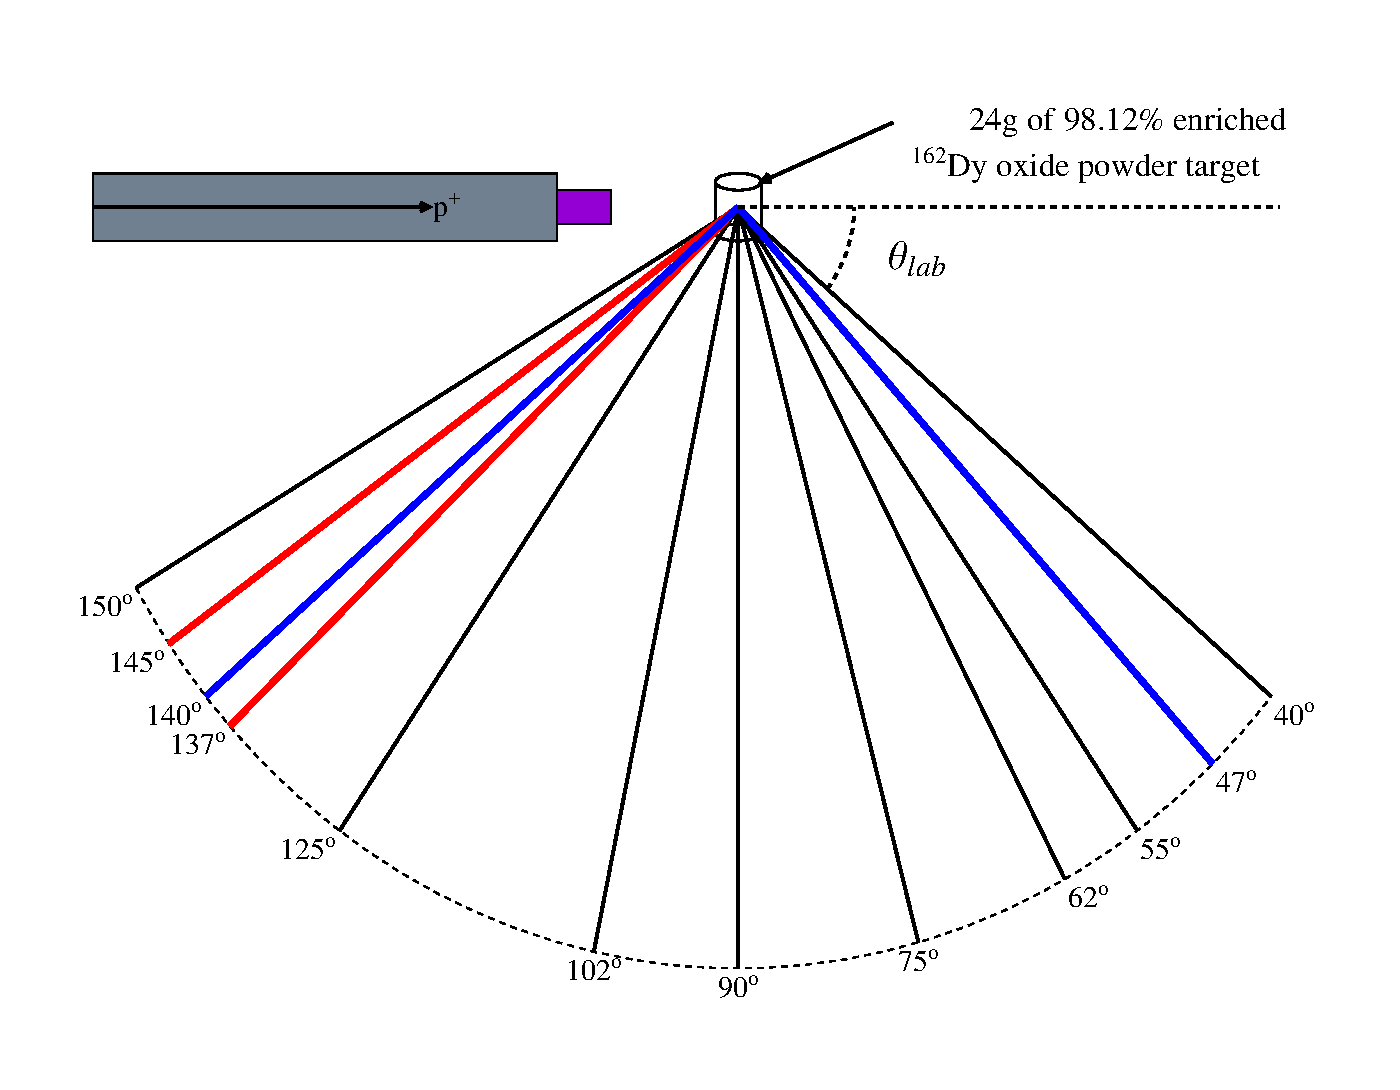
\includegraphics[width=0.95\textwidth]{SciDraw_angular_distributions.eps}
\caption{Angles used in $^{162}$Dy(n,n$^\prime\gamma$) angular distributions. Angles in black are used in all measurements, while angles in red (137$^o$ and 145$^o$) are used for the E$_n$=1.6~MeV measurements and angles in blue are used for both E$_n$=2.2 and 3.1~MeV datasets. \label{fig:SciDraw_angular_distributions}}
\end{figure}

Once data is collected for both experimental campaigns, we carry out the analysis process to extract the various experimental quantities needed for nuclear structure studies (lifetimes of excited states, branching ratios/absolute intensities of $\gamma$-rays, etc) outlined in \S \ref{chp:Analysis}.
  %
% Chapter 3
%

\chapter{DATA ANALYSIS} \label{chp:Analysis}

\section{Calibrations and Corrections}
In order to account for systematic errors inherent to the laboratory, several corrections and calibrations must be made to ensure proper $\gamma$-ray spectroscopy. A suite of in-beam ($^{24}$Na \& $^{60}$Co) and offline calibration ($^{226}$Ra \& $^{152}$Eu) sources were implemented during the experimental campaigns to provide the numerous corrections that must be made; successful calibration hinges on the implementation of a wide energy range of strong calibration lines that do not shift. An ADC nonlinearity, a detector efficiency, and a target sample self-absorption correction are all applied to energy calibrated spectra before the analysis of data can begin.

\subsection{Energy Calibrations}\label{sec:energy_calibrations}
Proper energy calibration is vital to the success of DSAM lifetime measurements; the precision in peak centroid location determines the sensitivity of the lifetime  measurement, as centroid energy shifts for longer-lived levels ($\sim$1~ps) can be as small as 20~eV. With its large range of energetic decays (from 185~keV to 2.4~MeV shown in Table \ref{tab:226Ralines}), $^{226}$Ra is an ideal candidate to energy calibrate our spectra; the $^{226}$Ra spectrum from the $^{162}$Dy(n,n$^\prime\gamma$) experiments can be seen in Figure \ref{fig:226Ra_spectrum}. Angular distribution measurements saw the presence of an in-line calibration source in the form of annular-shaped ring of $^{23}$Na that had been irradiated with a separate, on-site neutron source to produce radioactive $^{24}$Na. The $\beta$-decay to $^{24}$Mg$^*$ leads to a cascade of two intense $\gamma$-rays, 1368.626 and 2754.007~keV, providing a calibration point at a higher energy than a typical $^{60}$Co source can provide (1173.228 \& 1332.492~keV). This sodium ring is placed around the detector crystal to ensure the two calibration $\gamma$-rays are not attenuated by the passive shielding from the experimental setup shown in Figure \ref{fig:ExpSetup}. While far from an ideal candidate for an energy calibration point, radioactive $^{28}$Al from a $^{27}$Al(n,$\gamma$) channel will emit a high intensity $\gamma$-ray at 1778.785~keV; this peak originates from the aluminum housing for the HPGe detector and is often not well-defined in width, especially compared to the traditional Radium and Cobalt sources normally used, and as such, the $^{28}$Al should not be a main energy calibration point. A table of all online and offline calibrations used in the $^{160}$Gd and $^{162}$Dy experiments can be found in Table \ref{tab:calib_params}. 

\begin{landscape}
\begin{table}[ht]
% \centering
\begin{center}
\caption{CALIBRATION LINES: $^{226}$RA DECAY-CHAIN \label{tab:226Ralines}}

% $^{226}$Ra decays\\
% \makebox[\textwidth]{
\begin{tabular}{c|c||c|c||c|c||c|c}
\hline
E$_\gamma$ (keV) & I$_\gamma$ (rel) & E$_\gamma$ (keV) & I$_\gamma$ (rel) & E$_\gamma$ (keV) & I$_\gamma$ (rel) & E$_\gamma$ (keV) & I$_\gamma$ (rel)  \\
\hline \hline
186.053(4)  &  3.502(28)  & 487.090(70)  &  0.431(6)   & 1120.287(10) &  14.66(103) & 1661.280(60)  &  1.063(17) \\ \hline
241.997(3)  &  7.130(50)  & 580.130(30)  &  0.369(6)   & 1155.190(20) &  1.611(19)  & 1729.595(15)  &  2.791(22) \\\hline
258.870(40) &  0.525(5)   & 609.312(7)   &  44.83(314) & 1238.110(12) &  5.750(46)  & 1764.494(14)  &  15.03(105) \\\hline
274.800(50) &  0.472(6)   & 665.453(22)  &  1.506(12)  & 1280.960(20) &  1.411(16)  & 1847.420(25)  &  1.994(20) \\\hline
295.224(2)  &  18.09(127) & 768.356(10)  &  4.780(38)  & 1377.669(12) &  3.895(31)  & 2118.550(30)  &  1.137(11) \\\hline
351.932(2)  &  35.04(245) & 785.960(90)  &  1.097(12)  & 1385.310(30) &  0.782(9)   & 2204.210(40)  &  4.820(39) \\\hline
455.000(70) &  0.287(6)   & 806.174(18)  &  1.250(13)  & 1401.500(40) &  1.311(12)  & 2293.400(120) &  0.298(8) \\\hline
480.430(20) &  0.336(5)   & 934.061(12)  &  3.041(24)  & 1509.228(15) &  2.065(31)  & 2447.860(100) &  1.525(14) \\
\end{tabular}
% }\\ 
\vspace{10pt}
\end{center}
Energies (in keV) and relative intensities (in arbitrary units) for $\gamma$-ray emissions from the $^{226}$Ra decay chain used in data calibrations for this work.
\end{table}
\end{landscape}

\begin{figure}[ht]
\begin{center}
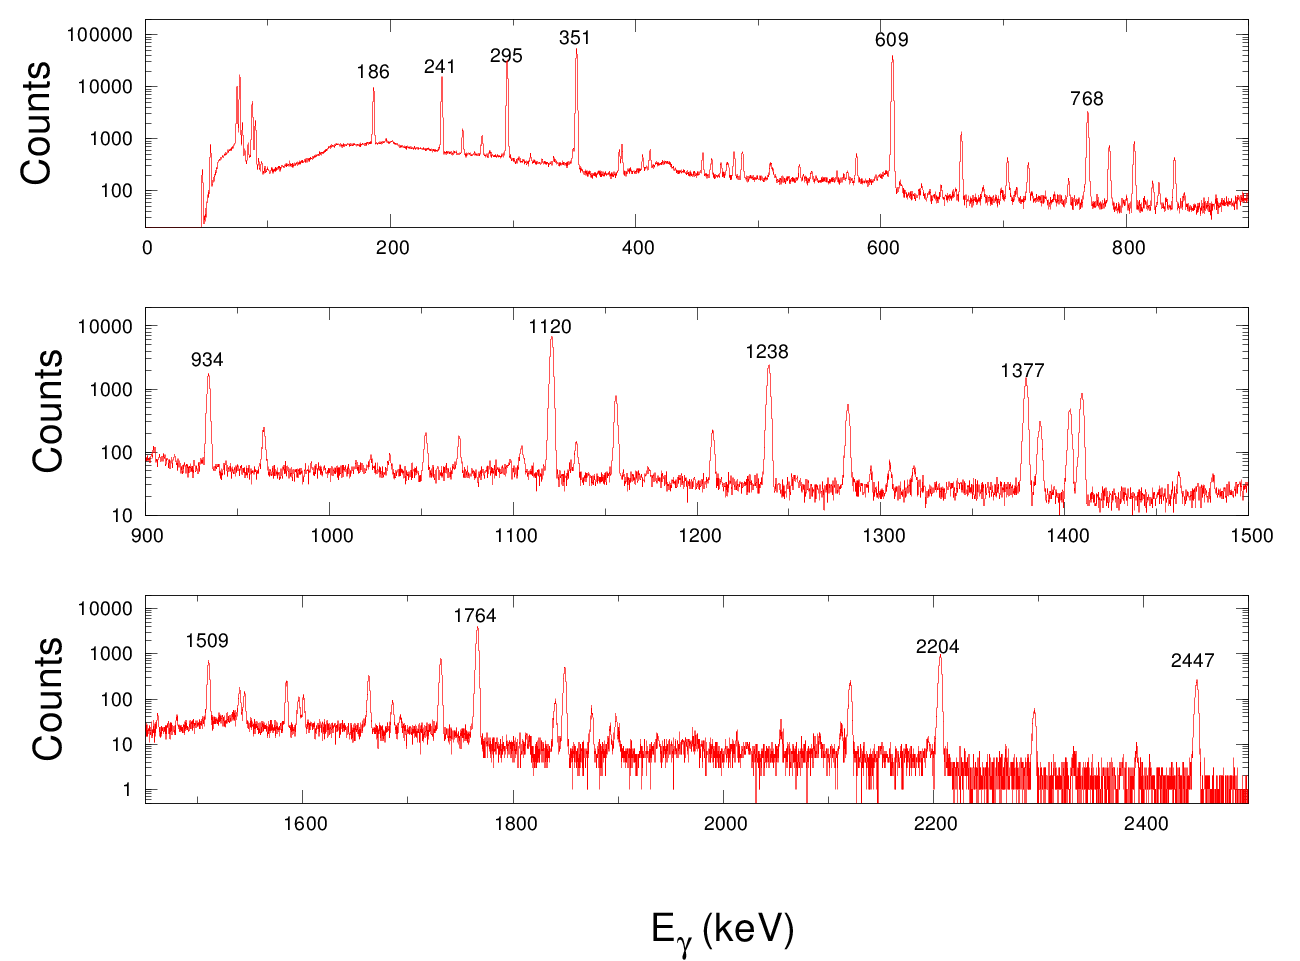
\includegraphics[width=0.95\textwidth]{calibration_226Ra.png}
\end{center}
\caption{Spectrum from a $^{226}$Ra calibration run during the $^{162}$Dy experiments. Sampled, higher intensity peaks are labeled by their energy in keV (refer to Table \ref{tab:226Ralines}).\label{fig:226Ra_spectrum}}
\end{figure}

\begin{landscape}
\begin{table}[ht]
% \centering
\begin{center}
\caption{ENERGY CALIBRATIONS: $^{160}$GD AND $^{162}$DY \label{tab:calib_params}} 

$^{160}$Gd(n,n$^\prime\gamma$) calibration E$_\gamma$ (keV)\\
% \makebox[\textwidth]{
\begin{tabular}{c|c|c|c|c|c|c}
\hline
\hline
E$_n$=1.5~MeV & 1173.228 & 1332.492  & 2223.245  \\ 
\hline
E$_n$=2.0~MeV &  1173.228 & 1332.492  & 2223.245    \\ 
\hline
E$_n$=2.8~MeV  &  1173.228 & 1332.492  & 1778.885 & 2223.245    \\ 
\hline
Excitation Function & 185.002 & 351.932 & 609.312 & 1120.287 &  1764.494 & 2223.245  \\ 
\end{tabular}
% }

\vspace{5mm}
% \centering
$^{162}$Dy(n,n$^\prime\gamma$) calibration E$_\gamma$ (keV)\\
% \makebox[\textwidth]{
\begin{tabular}{c|c|c|c|c|c|c|c|c}
\hline
\hline
E$_n$=1.6~MeV & 185.002 &  1173.228 & 1332.492 &  2223.245  \\ 
\hline
E$_n$=2.2~MeV & 185.002 &   1173.228 & 1332.492 &   2223.245    \\ 
\hline
E$_n$=3.1~MeV  & 351.932 & 609.312 & 1120.287 & 1173.228 & 1332.492 & 1764.494 & 2223.245 & 2754.007  \\ 
\hline
Excitation Function & 185.002 & 351.932 & 609.312 & 1120.287 &   1764.494 & 2223.245  \\ 
\end{tabular}
% }\\ 
\vspace{10pt}
\end{center}
Calibration points used for all $^{160}$Gd and $^{162}$Dy spectra energy calibrations, given in keV.
\end{table}
\end{landscape}

The linear energy calibrations from the $^{162}$Dy(n,n$^\prime\gamma$) experiments can be seen in figure \ref{fig:energy_calib}:

\begin{figure}[ht]
\begin{center}
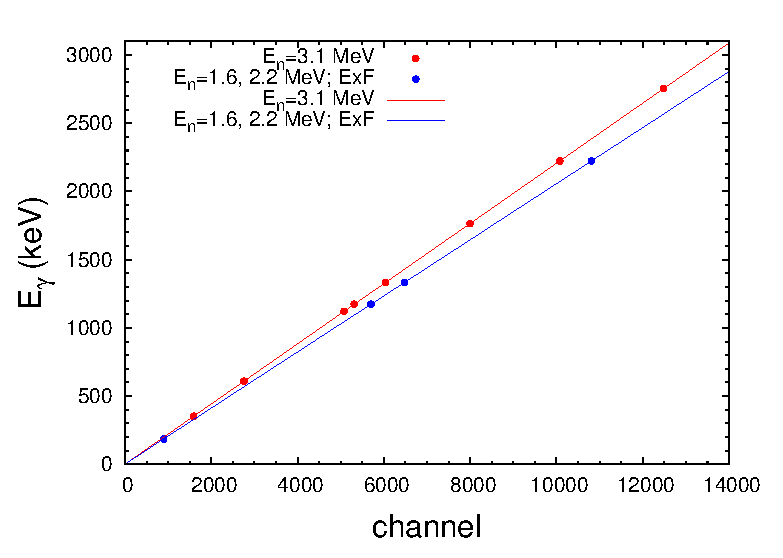
\includegraphics[width=0.97\textwidth]{310_energy_calib.eps}
\caption{Linear energy calibration, taken from the three $^{162}$Dy(n,n$^{\prime}\gamma$) angular distributions and single excitation function (ExF in the legend).}
\label{fig:energy_calib}
\end{center}
\end{figure}

The difference in linear energy calibrations is the result of a change in gain settings between the two $^{162}$Dy experiments; the excitation function measurements and E$_n$=1.6 \& 2.2~MeV angular distributions occurred in August of 2013, while the single E$_n$=3.1~MeV angular distribution took place months later, in March of 2014. The specific difference in energy calibration can be seen in Figure \ref{fig:energy_calib}, where the electronics gain settings were changed (a natural, necessary, and sometimes unintentional occurrence in the laboratory). %The molar quantity of stable target material used in the DSAM experiments means we are not constrained by any natural radioactivity of the sample.

\subsection{Nonlinearity Calibrations}\label{sec:nonlinearity_calibration}
The first of these corrections is an ADC nonlinearity calibration, where a binning nonlinearity is introduced in the data acquisition's ADC. In the ideal case, an ADC correlates an analog voltage to a specific bin (in this case, the energy of a $\gamma$-ray on the absissca), with the bins being equally spaced and sized. We, of course, do not live in a perfect world, and some bins cover a larger energy range than others, generating an easily correctable error in the measurement of peak centroids. To perform this offline correction, a radioactive $^{226}$Ra source is placed at the same location the target is suspended, and is allowed to decay. Since the multitude of decays from $^{226}$Ra have very well defined and precise centroids, we can compare the measured position of these peaks to literature values for the peak centroids. By plotting a relationship between the change in channel as a function of energy, we can generate the specific nonlinearity curve to make the correction. Generally, the nonlinearity correction introduces a $\pm$2 channel difference (at most a 0.5~keV correction), and this nonlinearity can be fit to an order 5 polynomial, shown in Figure \ref{fig:dsnonlin}:

\begin{figure}[ht]
\begin{center}
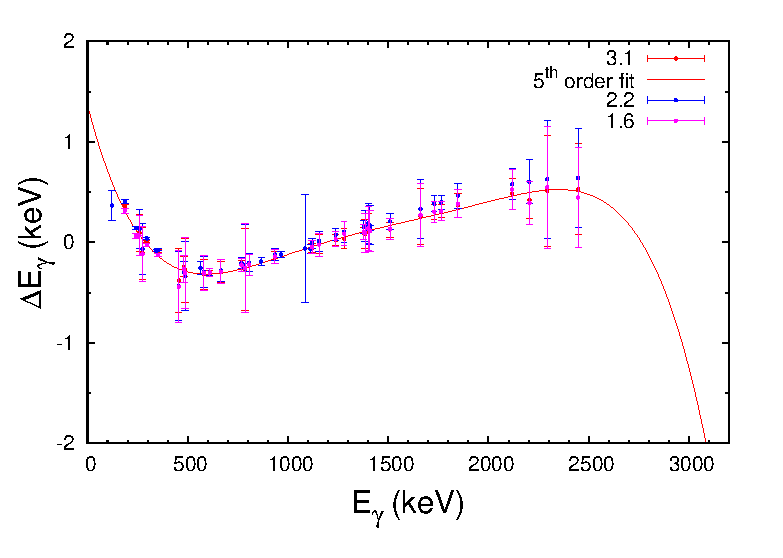
\includegraphics[width=0.97\textwidth]{310_dsnonlin_color.eps}
\caption{Order-5 polynomial nonlinearity correction, taken from the $^{162}$Dy(n,n$^{\prime}\gamma$) angular distribution with E$_n$=3.1~MeV}
\label{fig:dsnonlin}
\end{center}
\end{figure}
Special care must be taken to ensure a realistic polynomial fit for the ADC nonlinearity; polynomials of high order can gravely mis-characterize the ADC behavior outside of the range of calibration points used (in our case, $^{226}$Ra decays). In Figure \ref{fig:dsnonlin}, the downward turn in the fifth-order extrapolation above 2.5~MeV $\gamma$-rays would be magnified for higher order odd polynomials, and would turn upward (at a similarly unrealistic rate) for the even polynomials. To justify the use of an order-5 polynomial, the highest energy $\gamma$-ray observed in the $^{162}$Dy experiments is a 2779~keV de-excitation, keeping in line with a $\sim\pm$1~keV nonlinearity correction.
\subsection{Efficiency Calibrations}\label{sec:efficiency_calibration}
High Purity Germanium detectors have an intrinsic detection efficiency, dependent on the energy of a particular $\gamma$-ray that enters the Ge crystal; higher energy $\gamma$-rays have a lower probability of depositing their entire energy into the detector, so this must be accounted for in angular distribution data to get correct $\gamma$-ray intensities. The same spectrum from the nonlinearity calibrations is used, as we can simply compare the measured intensities of $\gamma$-rays from the $^{226}$Ra source to the literature values of $\gamma$-ray intensity. This efficiency correction is shown in Figure \ref{fig:polyfit} as a function of \textit{E$_\gamma$}:

\begin{figure}[ht]
\begin{center}
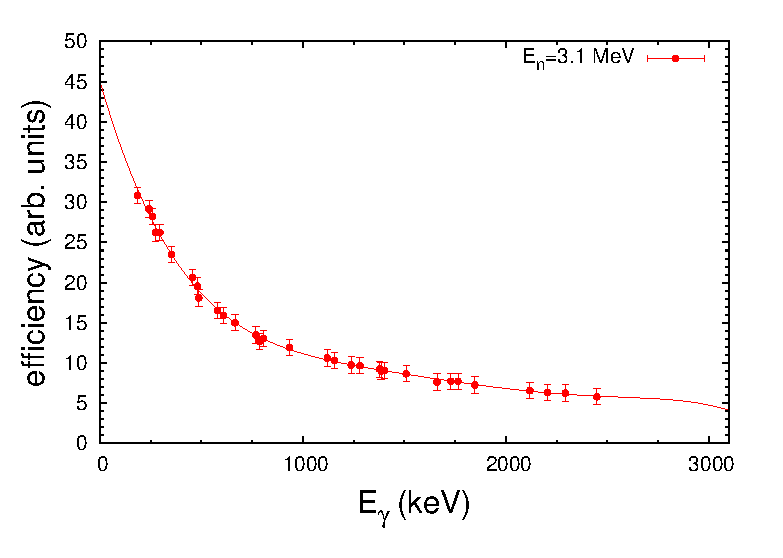
\includegraphics[width=0.97\textwidth]{310_polyfit_color.eps}
\caption{Fifth-order relative efficiency curve taken from the $^{162}$Dy(n,n$^{\prime}\gamma$) angular distribution with E$_n$=3.1~MeV
\label{fig:polyfit}}
\end{center}
\end{figure}

\subsection{Self-Absorption Corrections}\label{sec:gambit_correction}
One of the key characteristics of the Winterbon formalism for determining \textit{F}(\textit{$\tau$}) as a funciton of \textit{$\tau$} is the use of large quantities of target material to provide sufficient nuclear and electronic stopping power \cite{WINTERBON_1975}. Of course, a downside to using these molar quantities of powder targets is that incoming neutrons and outgoing $\gamma$-rays will be attenuated by the physical thickness of material. Much like the efficiency calibration, the self-absorption correction must be made to get proper $\gamma$-ray intensities, since low-energy gamma rays may be drastically attenuated by the thickness of the sample. Both the physical geometry of the experimental setup and size of the sample affect this highly-angular dependent correction, used solely in the angular distribution data in the presented analysis. The {\tt GAMBIT} (\cite{ENGELBRECHT1970187}, \cite{CONTE_NUMERICAL_text}, \cite{GAMBIT_BORING1960}) codes and subroutines are well-equipped to perform this correction for any experiment performed at UKAL involving a cylindrical target cell; {\tt GAMBIT} takes into account differential elastic neutron cross sections (\textit{$\frac{d\sigma_n}{d\Omega}$} at 0$^\circ$ and 180$^\circ$), total neutron cross sections ($\sigma_{n,\textit{tot}}$), elastic neutron scattering cross sections ($\sigma_{n,\textit{el.}}$), and the photon absorption cross sections ($\sigma_{\gamma}$ for each composite material found in the sample ($^{162}$Dy$_2^{16}$O$_3$). Figure \ref{fig:gambit} shows the multiplicative factor needed to give the correct peak areas from this self-absorption of $\gamma$-rays as a function of $\theta_{lab}$. Factors near unity indicate little to no correction is needed (at higher energies, a $\gamma$-ray can easily escape the physical target), while a significant correction must be made to low-energy ($<$200 keV) $\gamma$-rays that are partially or heavily attenuated by the sample. 

\begin{figure}[ht]
\begin{center}
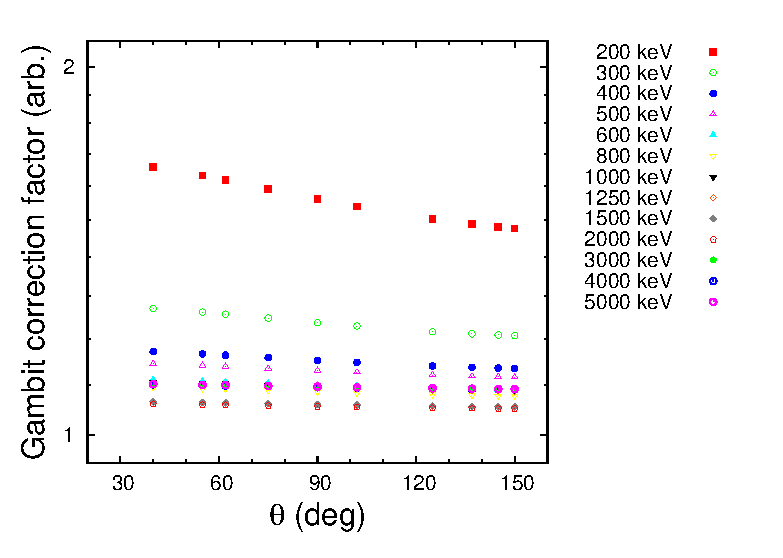
\includegraphics[width=0.97\textwidth]{gambit.eps}
\caption{Multiplicative factor calculated by {\tt GAMBIT} to correct for the angular dependent $\gamma$-ray self-absorption by a finite-size target. \label{fig:gambit}}
\end{center}
\end{figure}

This self-absorption correction given by {\tt GAMBIT} is sufficient and appropriate for use in the (n,n$^\prime\gamma$) experiments at UKAL, even though much more modern approaches to characterize the self-absorption exist. Molecular dynamics calculations can be made to generate this angularly and energetically dependent attenuation, but require a much higher amount of computational power to complete. Since the newer, refined methods do not offer a more efficient or accurate self-absorption calculation, we can confidently use the more simplistic approach given by the {\tt GAMBIT} code.

\section{Statistical Analysis}
The wealth of information that can be extracted from $\gamma$-ray spectroscopy hinges on consistent, precise statistical analysis of spectra. An example of a properly TOF gated, energy calibrated, and background subtracted spectrum can be seen in Figure \ref{fig:examplespec}:

\begin{figure}[h]
\begin{center}
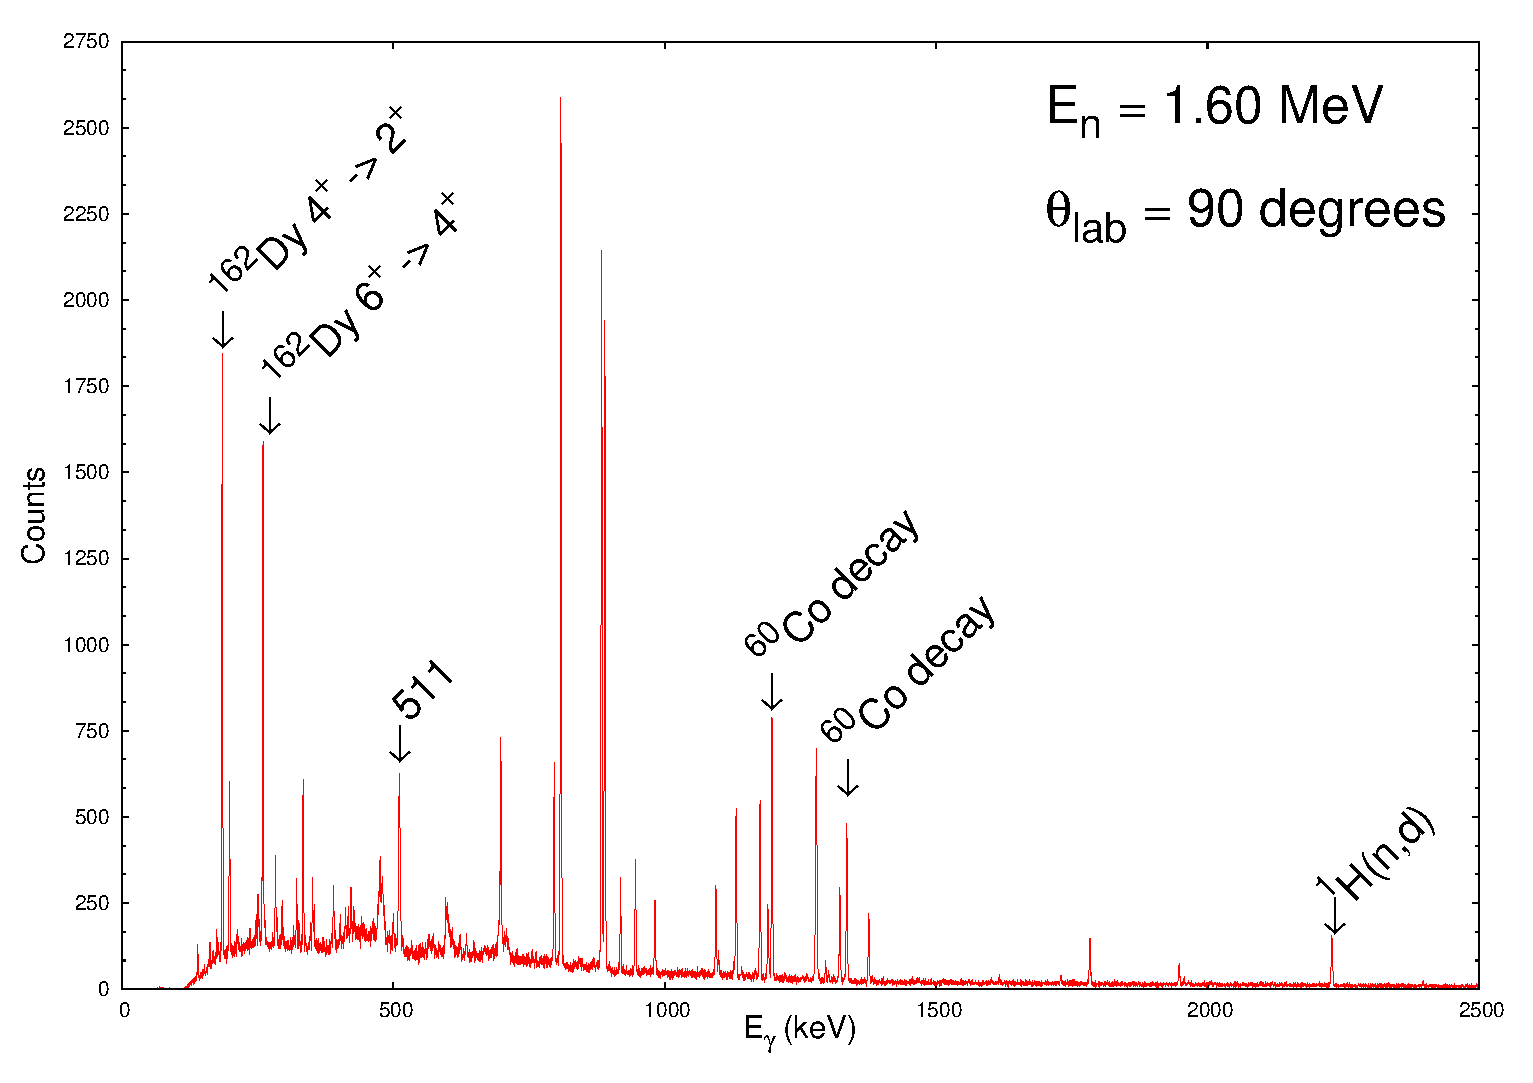
\includegraphics[width=0.95\textwidth]{samplespec.eps}
\caption{Example of an energy-calibrated spectrum from the $^{162}$Dy angular distribution at E$_n$=1.6~MeV and $\theta_{lab}$=90$^\circ$, outlining typical background levels and miscellaneous $\gamma$-ray transitions.
\label{fig:examplespec}}
\end{center}
\end{figure}

\subsection{Fitting Procedures}\label{sec:fitting_procedures}
A $\gamma$-ray event recorded in the HPGe detector will manifest itself as a skewed, defined-width gaussian distribution on the histogram of the form shown in Equation \ref{eq:gaussian}, and is fit according to:

\begin{equation}\label{eq:gaussian}
y=\sum_k \frac{A_k}{(2\pi)^\frac{1}{2}\sigma}e^{-\frac{1}{2}\left(\frac{Z-Z_k}{\sigma}\right)^2}\left[1+P_{left,1}\left(\frac{Z-Z_k}{\sigma}\right)^4+P_{left,2}\left(\frac{Z-Z_k}{\sigma}\right)^{12}\right]
\end{equation}

The multiple parameter fitting procedure in Equation \ref{eq:gaussian} can be qualitatively described as measures of \textit{$\sigma$}, the width of the peak, \textit{Z$_k$}, the centroid location of a peak, \textit{A$_k$}, the peak height, and two parameters relating to the low-energy tail (a measure of the skewedness of the gaussian), \textit{P$_{left,1}$} \& \textit{P$_{left,2}$}. This trailing edge is the result of Bremsstrahlung escape from the detector itself \cite{Knoll_text}, but is necessary to accurately fit low-intensity peaks that exist as a doublet with higher-intensity peaks. For a given peak, three parameters are interpolated separately into a $\chi^2$ fit, the width, $\sigma$, and the two left-polynomial terms, \textit{P$_{left,1}$} \& \textit{P$_{left,2}$}. Typically, the polynomial terms are a small, but significant contribution (\textit{P$_{left,1}$}$<$0.010), and $\sigma$ is bounded between $\sim$2 and $\sim$7 channels ($\sim$0.5 to $\sim$1.5~keV energy resolution). These open parameters are iteratively fit one at a time to best recreate the shape of the gaussian distribution in the histogram; once all peaks have been properly fitted, the fit parameters are exported to a peak list with peak areas, centroids (subsequently the energy of the $\gamma$-ray), and the associated statistical errors from each parameter. \textit{F$_i$tP$_i$c} \cite{FitPic_Fribourg} was used to interpolate fit parameters for all experimental data in both $^{160}$Gd and $^{162}$Dy. Peaks are assigned to groups with up to five other peaks to ensure a locally linear background for each gaussian. 
\subsection{Observable Extraction}
From the peak list, we can extract a wealth of knowledge about the decay radiation observed, even with the seemingly basic information gained from fitting the peaks in a given histogram.
\subsubsection{Excitation Functions}\label{sec:excitation_functions}
Although no direct measurable quantities ($\gamma$-ray energies, branching ratios, etc) can be extracted from the excitation function data, previously unplaced $\gamma$ rays can be assigned to de-exciting levels simply by looking at the raw threshold of $\gamma$-ray population. Two plots per $\gamma$-ray are generated, the relationship between E$_\gamma$ and E$_n$, and peak area as a function of E$_n$; the first plot allows confirmation that each peak is fit uniformly, where the relationship between peak area and neutron energy will allow us to determine an approximate threshold energy. Any modulation of the $\gamma$-ray energy as a function of bombarding neutron energy is a signature of non-uniform peak fitting or that another $\gamma$-ray of similar energy has been populated in the level scheme at a different threshold. When this latter case occurs, the peak area as a funciton of neutron energy will also show a corresponding bump at the same threshold. An example of this ensemble of plots is shown in Figure \ref{fig:sample_exf}:


\begin{figure}[h!]
\begin{center}
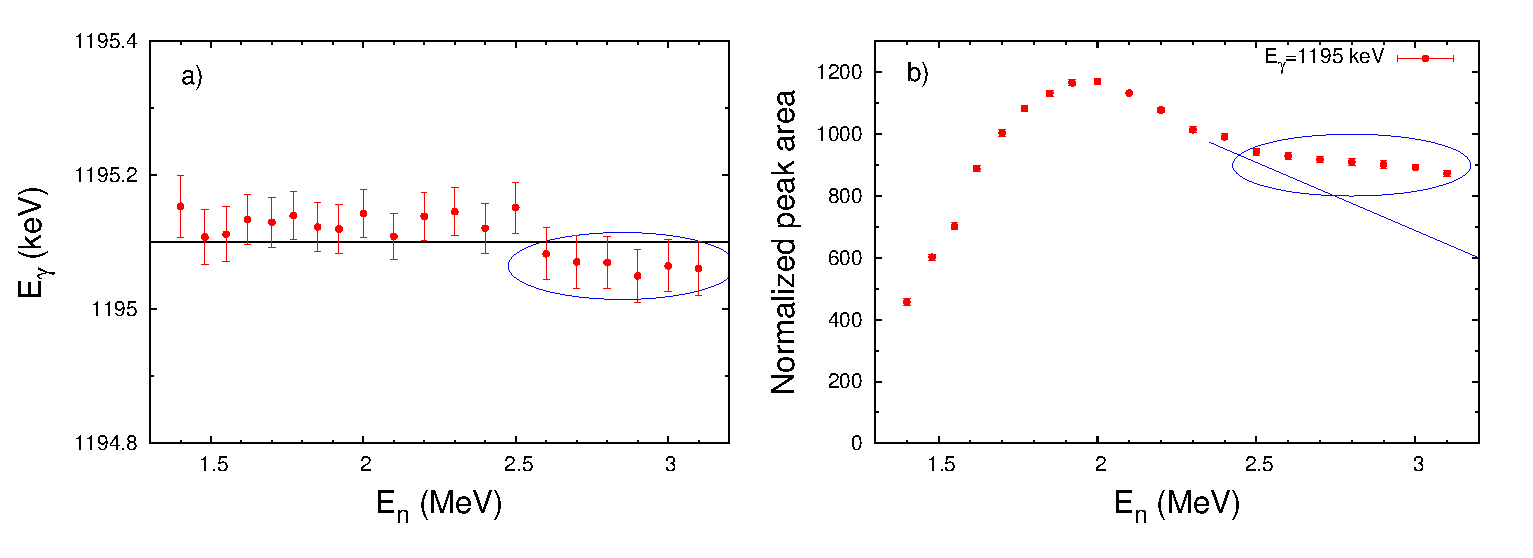
\includegraphics[width=0.97\textwidth]{sample_exf.eps}
\caption{A set of plots from a typical excitation function for a single $\gamma$-ray transition, in `a)', E$_\gamma$ vs. E$_n$, and in `b)', the peak area vs E$_n$. Note the dip in $\gamma$-ray energy at 2.6~MeV, and corresponding bump in peak area (shown as a blue ellipse to guide the eye), indicating a second transition of a similar (slightly lower) energy being populated.
\label{fig:sample_exf}}
\end{center}
\end{figure}

The absolute threshold energies for $\gamma$-rays are used to determine where a $\gamma$-ray comes in, and to determine which level is providing the de-excitation, a problem that would otherwise require $\gamma$-$\gamma$ coincidence measurements. Since the excitation functions give $\gamma$-ray placements in the nucleus, we are no longer reliant on the more complex coincidence measurements. 

Figure \ref{fig:ExF_difference_140_230} shows an example of the population rate of a $\gamma$-decay in $^{162}$Dy by superimposing multiple neutron energy spectra on top of each other. Take note that the E$_n$=1.4 and 1.7~MeV datasets are below the energy threshold of the level that the 1647~keV decay leaves, with a sharp increase of counted statistics just above the level energy threshold, growing until a well-defined gaussian peak is seen at E$_n$=2.3~MeV.

\begin{figure}[h!]
\begin{center}
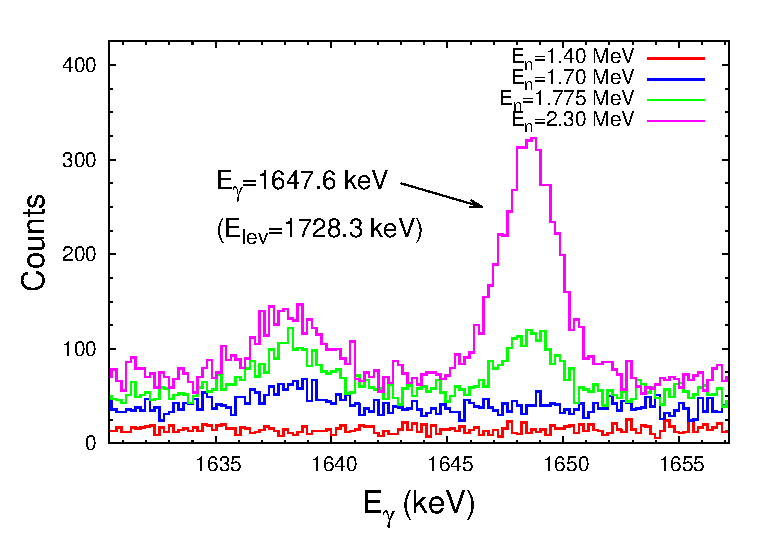
\includegraphics[width=0.97\textwidth]{ExF_difference_140_230.eps}
\caption{Spectra from four bombarding neutron energies (E$_n$=1.4, 1.7, 1.775, and 2.3~MeV datasets) to show the typical increase of statistics for a single peak, a 1647~keV decay from the 1728~keV state in $^{162}$Dy. Note the peak area emerge just above the level energy threshold (1.775~MeV neutron dataset), with optimal statistics in the E$_n$=2.3~MeV set.
\label{fig:ExF_difference_140_230}}
\end{center}
\end{figure}

Proper placement of $\gamma$-rays in the level scheme is vital to confident, precise measurement of level lifetimes, absolute intensities, and multipole mixing fractions. Although the experiments at UKAL are not designed to find new J=0 states (\textit{e.g.} something the Q3D spectrometer can better achieve with two nucleon transfer reactions), tentative spin assignments and/or confirmation of spin can be placed with information from both the excitation functions and angular distributions. J=0 excitations should have a threshold very close to the energy of the state, as there is very little angular momentum needed to populate the state, and since inelastic neutron scattering can only realistically populate up to spin 5$^\pm$ states (a consequence of the limited angular momentum transfer from the spin-$\frac{1}{2}$ neutron to the nucleus during inelastic scattering), stringent upper limits on the spin and parity of a parent level can be placed by examining the spin and parity of the daughter state. For example, if a transition between two levels is energetically feasible, we know that the spin and parity of the parent state will be within $\pm$2 units of angular momentum of the daughter level because only $\Delta$J$<$2 multipolarities are observed in the laboratory with any appreciable or measurable intensity, as the relative intensity of E3, E4 and higher multipolarities are orders of magnitude less intense than the strong E2 quadrupole radiation observed in the lab.  For example, in cases where the daugher level is spin-5, we know that the parent state will be spin-3 or spin-4, due to the low spin-population of inelastic neutron scattering. 

%[ENERGY THRESHOLDS TO PLACE UNASSIGNED GAMMA RAYS]
\subsubsection{Angular Distributions}\label{sec:AD_Ft}
Spectra from the angular distributions have all corrections applied (nonlinearity, detector efficiency, and self-absorption), where the peak list is separated and sorted into groups based on the $\gamma$-ray energy as a function of angle. Careful bounding of groups must be made to ensure good $\gamma$-ray separation in the event of a close-lying doublets, while maintaining sufficient overhead to account for large-order Doppler energy shifts (very short lifetimes on the order of $\sim$10~fs). 

%[TALK ABOUT ACTUAL CALCULATION OF F($\tau$) factor]
In order to extract the lifetime of a particular state, precise calculation of the theoretical values for \textit{F}(\textit{$\tau$}) (Winterbon curve) must be made to compare the extracted \textit{F}(\textit{$\tau$}) from the Doppler shifted $\gamma$-rays. This calculation is achieved via {\tt v1pgm}, which takes into account the calculated recoil velocity from Equation \ref{eq:betarecoil}, the target density and atomic weight of each element in the target, and a range of lifetimes to iterate over (from 1~fs to 10~ps). Since the target does not change composition or density, the only input parameter that changes is the nuclear recoil velocity, dependent solely on the bombarding neutron energy. The calculated Winterbon curves for the $^{162}$Dy experiments can be seen in Figure \ref{fig:ftau_all}, with an emphasis to highlight the ideal range ($\sim$10~-~$\sim$600~fs) to measure lifetimes with DSAM. In general, \textit{F}(\textit{$\tau$}) is constrained by the uncertainties in electronic and nuclear stopping powers, resulting in $\sim$10\% uncertainty in the attenuation factor \cite{Belgya_DSAM1996}; this uncertainty is propagated to the extracted lifetime's uncertainty.

\begin{figure}[ht]
\begin{center}
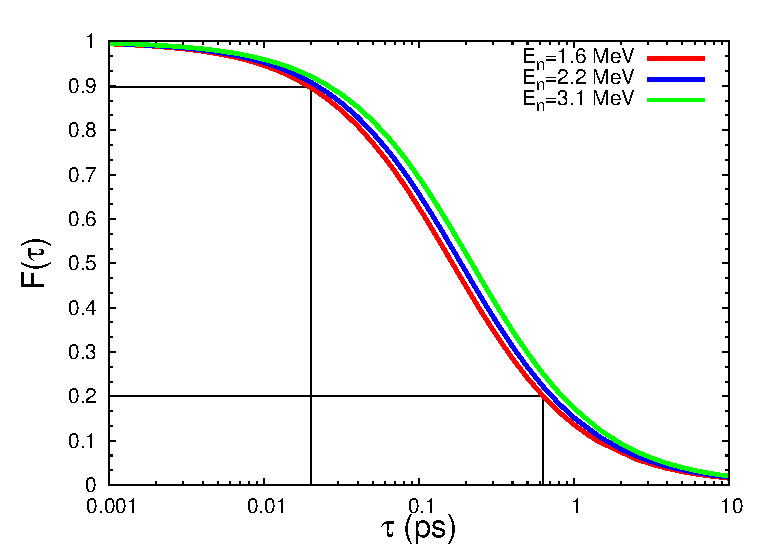
\includegraphics[width=0.97\textwidth]{ftau_all.eps}
\caption{Calculated Winterbon curves (\textit{F}(\textit{$\tau$}) as a function of \textit{$\tau$}) for E$_n$=1.6, 2.2, and 3.1~MeV $^{162}$Dy angular distributions. Sensitive lifetime ranges from DSAM are shown as vertical black lines, with the corresponding \textit{F}(\textit{$\tau$}) values as horizontal lines.
\label{fig:ftau_all}}
\end{center}
\end{figure}

Direct comparison of the experimental \textit{F}(\textit{$\tau$}) value to the calculated Winterbon curve for a particular $\gamma$-ray is straightforward; in Figure \ref{fig:DSAM_example}, the measured slope of the Doppler shift of 0.665 correlates to a \textit{$\tau$} of 21~fs. For excited states with only one de-exciting transition, the extracted $\gamma$-ray lifetime is equivalent to the level lifetime, where level lifetimes with multi-channel $\gamma$-ray de-excitations are extracted from the weighted average of all de-exciting \textit{F}(\textit{$\tau$}) values, weighted by the uncertainty in each measured F($\tau$). This standard statistical average can be explicitly seen in Equation \ref{eq:weighted_average} taken from \cite{Bevington_text}. Special care must be taken, however, to ensure accurate and precise Doppler shifts are obtained from the various de-excitation channels from a level. In several cases for low energy and/or intensity $\gamma$ rays, the shift (magnitude of F($\tau$)) will be negative or consistent with zero; in this case, any lifetime deduced from the Doppler shift is not accounted in the weighted average of the level lifetime. The same rules apply when a particular $\gamma$ ray has the potential to be coincident with a background line, where the F($\tau$) value may be unreliable. As a rule of thumb, F($\tau$) should be about 1$\sigma$ variance from zero to be considered a good candidate for DSAM, however, this is sometimes impossible if the physical lifetime is on the precipice of the sensitive range of lifetimes DSAM can measure. Large upper uncertainties are not uncommon for the near-picosecond lifetimes with `shallow' values for F($\tau$) measured with DSAM (e.g. 3000$^{+4800}_{-1300}$~fs for the 1666~keV state in $^{162}$Dy), yet another experimental challenge we must overcome when measuring the lifetimes of states.

\begin{equation}\label{eq:weighted_average}
\widehat{F(\tau)}=\frac{\sum_{i} F_i(\tau) \sigma^{-2}_i}{\sum_{i}\sigma^{-2}_i}, \sigma^2(\widehat{F(\tau)})=\frac{1}{\sum_i \sigma^{-2}_i}
\end{equation}

\begin{figure}[ht]
\begin{center}
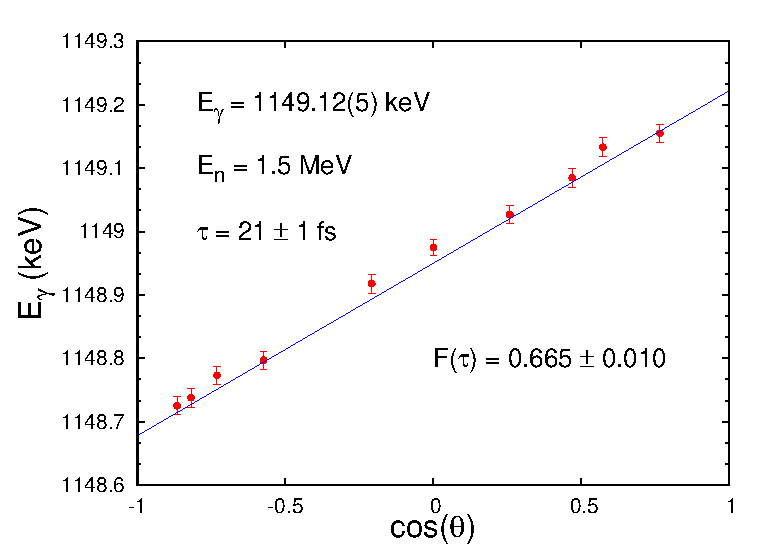
\includegraphics[width=0.97\textwidth]{DSAM_example.eps}
\caption{Example Doppler Shift for a 1149~keV $\gamma$-ray populated in the 1.5~MeV $^{160}$Gd(n,n$^\prime\gamma$) experiment. Here, the \textit{F}(\textit{$\tau$}) value of 0.665 $\pm$ 0.010 corresponds to a lifetime of 21 $\pm$ 1 fs.
\label{fig:DSAM_example}}
\end{center}
\end{figure}

Further refinement of any spin assignments made in the literature can be deduced by examining the a$_2$ and a$_4$ coefficients from Equation \ref{eq:angdistW}; isotropic or near-isotropic angular distributions could suggest significant multipole mixing of $\gamma$ radiation, as pure E2, E1, or M1 radiation will mimic the classical radiation patterns displayed in Figure \ref{fig:multipole_diff}. The decay radiation pattern leaving a 0$^+$ excitation will also be isotropic in the angular distribution, as this is the equivalent of an unaligned decaying state. The angular distributions can be used to confirm or deny tentative spin-0 states by examining the angular distribution, but this technique should not be used to find new 0$^+$ excitations (two nucleon transfer reactions are still a much higher resolution method). For all angular distributions presented in this work, the peak areas are normalized in a way to ensure the angular distribution of the decay from the first excited 0$^+$ state is isotropic (a$_2$ consistent with 0). This is justified in \cite{Lesher_160Gd0s}, where multiple angular distribution normalizations were examined: once with the above normalization, and once where we normalized the peak area to another tentative (now repudiated) 0$^+$ state with disastrous results. Under this secondary normalization, strong E2 transitions that show no mixing ceased to have the same qualitative shape of a pure quadrupole in Figure \ref{fig:multipole_diff}, implying this was not a suitable candidate for normalization (or as an isotropic 0$^+$ $\rightarrow$ 2$^+$ transition). Special care must also be taken with the evaluation of the angular distributions, as there are multiple ways to create an isotropic distribution, via proper mixing of multipole radiation (admixtures of E2 and M1 radiation).

If the angular distribution is not isotropic or indicative of a pure quadrupole or dipole radiation (Figure \ref{fig:multipole_diff}), then the $\gamma$-ray may be of a mixed multipolarity. This commonly occurs in transitions where J$^\pi_i$ $\approx$ J$^\pi_f$, but is not to be confused with an E0 monopole transition, which is strictly forbidden by $\gamma$ decay and must occur via internal conversion electrons. In order to characterize this mixing, we compare the a$_2$ and a$_4$ coefficients to theoretical calculations of the same a$_2$ and a$_4$ coefficients for a particular J$^\pi$ value for a level, assuming there is no mixing. The statistical model for a compound nucleus is used to calculate cross sections for a (n,n$^\prime\gamma$) reaction with the target nucleus being treated as an optical model potential (the combination of a real Woods-Saxon potential with a diffuse, imaginary Gaussian surface potential). The {\tt FORTRAN} code used to achieve this calculation is {\tt CINDY} (a Hauser-Feschbach formalism taken from \cite{SHELDON197399}). The multipole mixing fraction (effectively a$_2$ and a$_4$) is then varied in the statistical model to reproduce the angular distribution for a possible J$^\pi$; the direct comparison of experimental Legendre Polynomial coefficients to those calculated in this statistical model lead directly to $\chi^2$ as a function of $\delta$, the multipole mixing fraction. Any $\gamma$-ray observed in our experiments that has a known placement in the level scheme can be added to the optical model to perform this $\chi^2$ minimization, where the smallest value of $\chi^2$ corresponds to the optimal value of $\delta$ for a particular de-excitation. These experimental mixing fractions aid in the calculation of the reduced transition probabilities for mixed multipolarity $\gamma$ decays given in Equation \ref{eq:BE2exp}, also using Equations \ref{eq:FE2} or \ref{eq:FM1}. An example extraction of $\delta$ from the angular distribution of $\gamma$-rays can be seen in Figure \ref{fig:delta_mixing_example}; $\chi^2$ is minimized locally for this $\gamma$ ray at a $\delta$ value $\sim$1, which indicates $\sim$50\% E2/M1 mixing. In Figure \ref{fig:delta_mixing_example}, the top left plot shows the measured angular distribution of the 1308~keV $\gamma$ ray, with {\tt CINDY} calculations for a range of starting spins decaying to a spin-4 state. The intersection of the black ellipse and the colored ellipses (calculations) correspond to the projections in the bottom plot, where we verify the lowest $\chi^2$ value on the y-axis for a particular delta on the x-axis for the 4$^+\rightarrow$4$^+$ transition.

\begin{figure}[ht]
\begin{center}
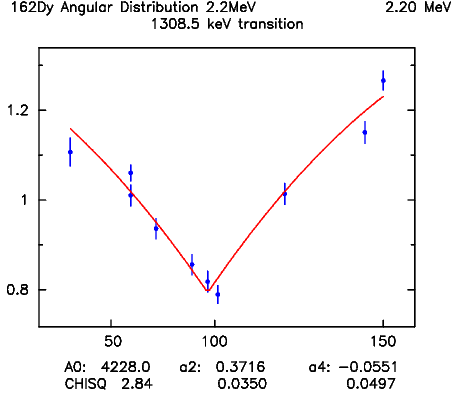
\includegraphics[height=0.25\textheight]{1308_AD_fit.png}
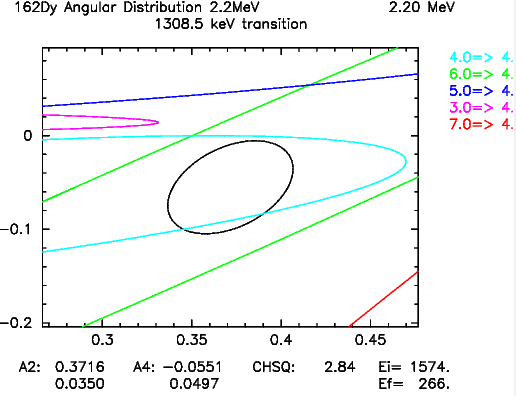
\includegraphics[height=0.25\textheight]{1308_AD_chisq_fit.png}\\
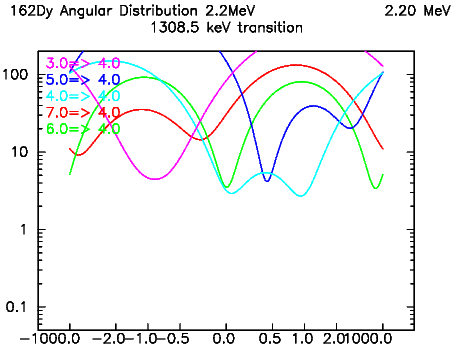
\includegraphics[width=0.73\textwidth]{1308_AD_delta_chi.png}\\
\caption{Example extraction of multipole mixing fraction ($\delta$) for a 4$^+\rightarrow$4$^+$ transition in $^{162}$Dy. Top-left plot: angular distribution of the 1308~keV $\gamma$ ray. Top-right plot: {\tt CINDY} comparison for a range of initial spins (color online) decaying to the final spin of 4; intersections with the black ellipse mark local/global minima of $\chi^2$ vs $\delta$. Bottom plot: projection of {\tt CINDY} comparison as $\chi^2$ as a function of $\delta$ minimization (note the lowest $\chi$ value corresponds to the $\delta\approx$1 for the cyan-colored 4$^+\rightarrow$4$^+$ transition). (color online) \label{fig:delta_mixing_example}}
\end{center}
\end{figure}
%add in an example figure of mixing and the chi squared minimzation process????
%possibly add in U=V+iW

To round out the cadre of important experimental information, we can extract the absolute intensity of $\gamma$-rays that de-excite the nucleus from the angular distribution data. The \textit{A$_o$} coefficient from Equation \ref{eq:angdistW} is proportional to the absolute intensity, and simply needs to have the efficiency \& self-absorption corrections applied to the measured \textit{A$_o$} (gross peak area). The branching ratios immediately follow from the absolute intensities, since we know all $\gamma$-decay channels open to a particular level, and these are used to calculate absolute transition probabilities (Equation \ref{eq:BE2exp}).



  \chapter{RESULTS}\label{sec:lifetime_inflation}
When reporting the lifetimes in this work, it is prudent to distinguish which bombarding neutron energy angular distribution is used, as the lifetimes are sensitive to inflation from multiple sources. First, recall Figure \ref{fig:ftau_all}, where we observe inflation of the extracted lifetimes due to the calculation of \textit{F}($\tau$) from a higher neutron energy, and thus, a modified value for the nuclear and electronic stopping powers that allows us to extract the lifetime. To minimize this effect, the neutron energy is carefully chosen under the time constraints imposed by accelerator availability. Specific neutron energies were selected with the aid of the excitation function measurements. Second, the extracted lifetime can be inflated due to level-feeding effects from higher-lying excitations in the nucleus; for these reasons, lifetimes are reported from the \textit{lowest} energy threshold possible to reduce this effect of observed lifetime inflation. As decays from higher-lying levels feed a state, the decay width (and thus lifetime) of the state are artificially inflated; this effect is observed throughout the most fundamental measurements of nuclear lifetimes \cite{Casten_text,Wong_text}. An example of the proportional lifetime inflation for two excited states caused by level-feeding and bombarding neutron energy differences can be seen in Figure \ref{fig:lifetime_inflation}. 

\begin{figure}[h!]
\begin{center}
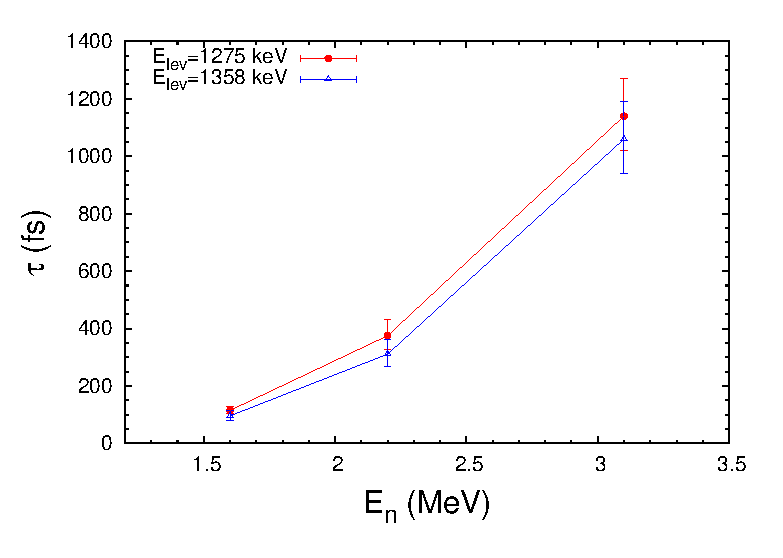
\includegraphics[width=0.85\textwidth]{lifetime_inflation_example.eps}
\caption{Lifetime inflation of the measured lifetimes for two levels (E$_{lev}$=1275~keV and E$_{lev}$=1358~keV) in $^{162}$Dy caused by effects due to a higher bombarding neutron energy and unknown level-feeding from higher-lying states. \label{fig:lifetime_inflation}}
\end{center}
\end{figure}

For the interest of discussion in \S \ref{chp:discussion}, lifetimes are separated into smaller, more digestable tables based on their corresponding discussion sections (\textit{e.g.} a table containing lifetimes of 0$^+$ states, one for the 2$^+_\gamma$ band, etc). Unless otherwise noted, tables in this chapter will contain experimentally determined level energies, $\gamma$-ray energies, branching ratios measured from our angular distributions, multipole mixing fractions where applicable, and the lifetime of the state with applicable uncertainties for all of the above quantities.
%preface to results being listed in preparation for discussion, separated by 
\section{$^{160}$Gd Results}
Results from the $^{160}$Gd campaign were published in \cite{Lesher_160Gd0s}, where this work also outlines and reiterates the major results taken from the suite of experiments in \S \ref{sec:Gd_exp}. A level scheme outlining all measured lifetimes in the $^{160}$Gd campaign is shown in Figure \ref{fig:160Gd_All}, with previously existing literature lifetimes in blue and new lifetime measurements in red. Prior to the presented results in this work, Gadolinium-160 has a complete paucity of lifetime information as a whole (most notably for 0$^+$ bands and negative parity bands), and as such, we add 29 new lifetimes, a factor of 7 increase, to the pool of placed literature values.

\begin{landscape}
\begin{center}
\begin{figure}[h!]
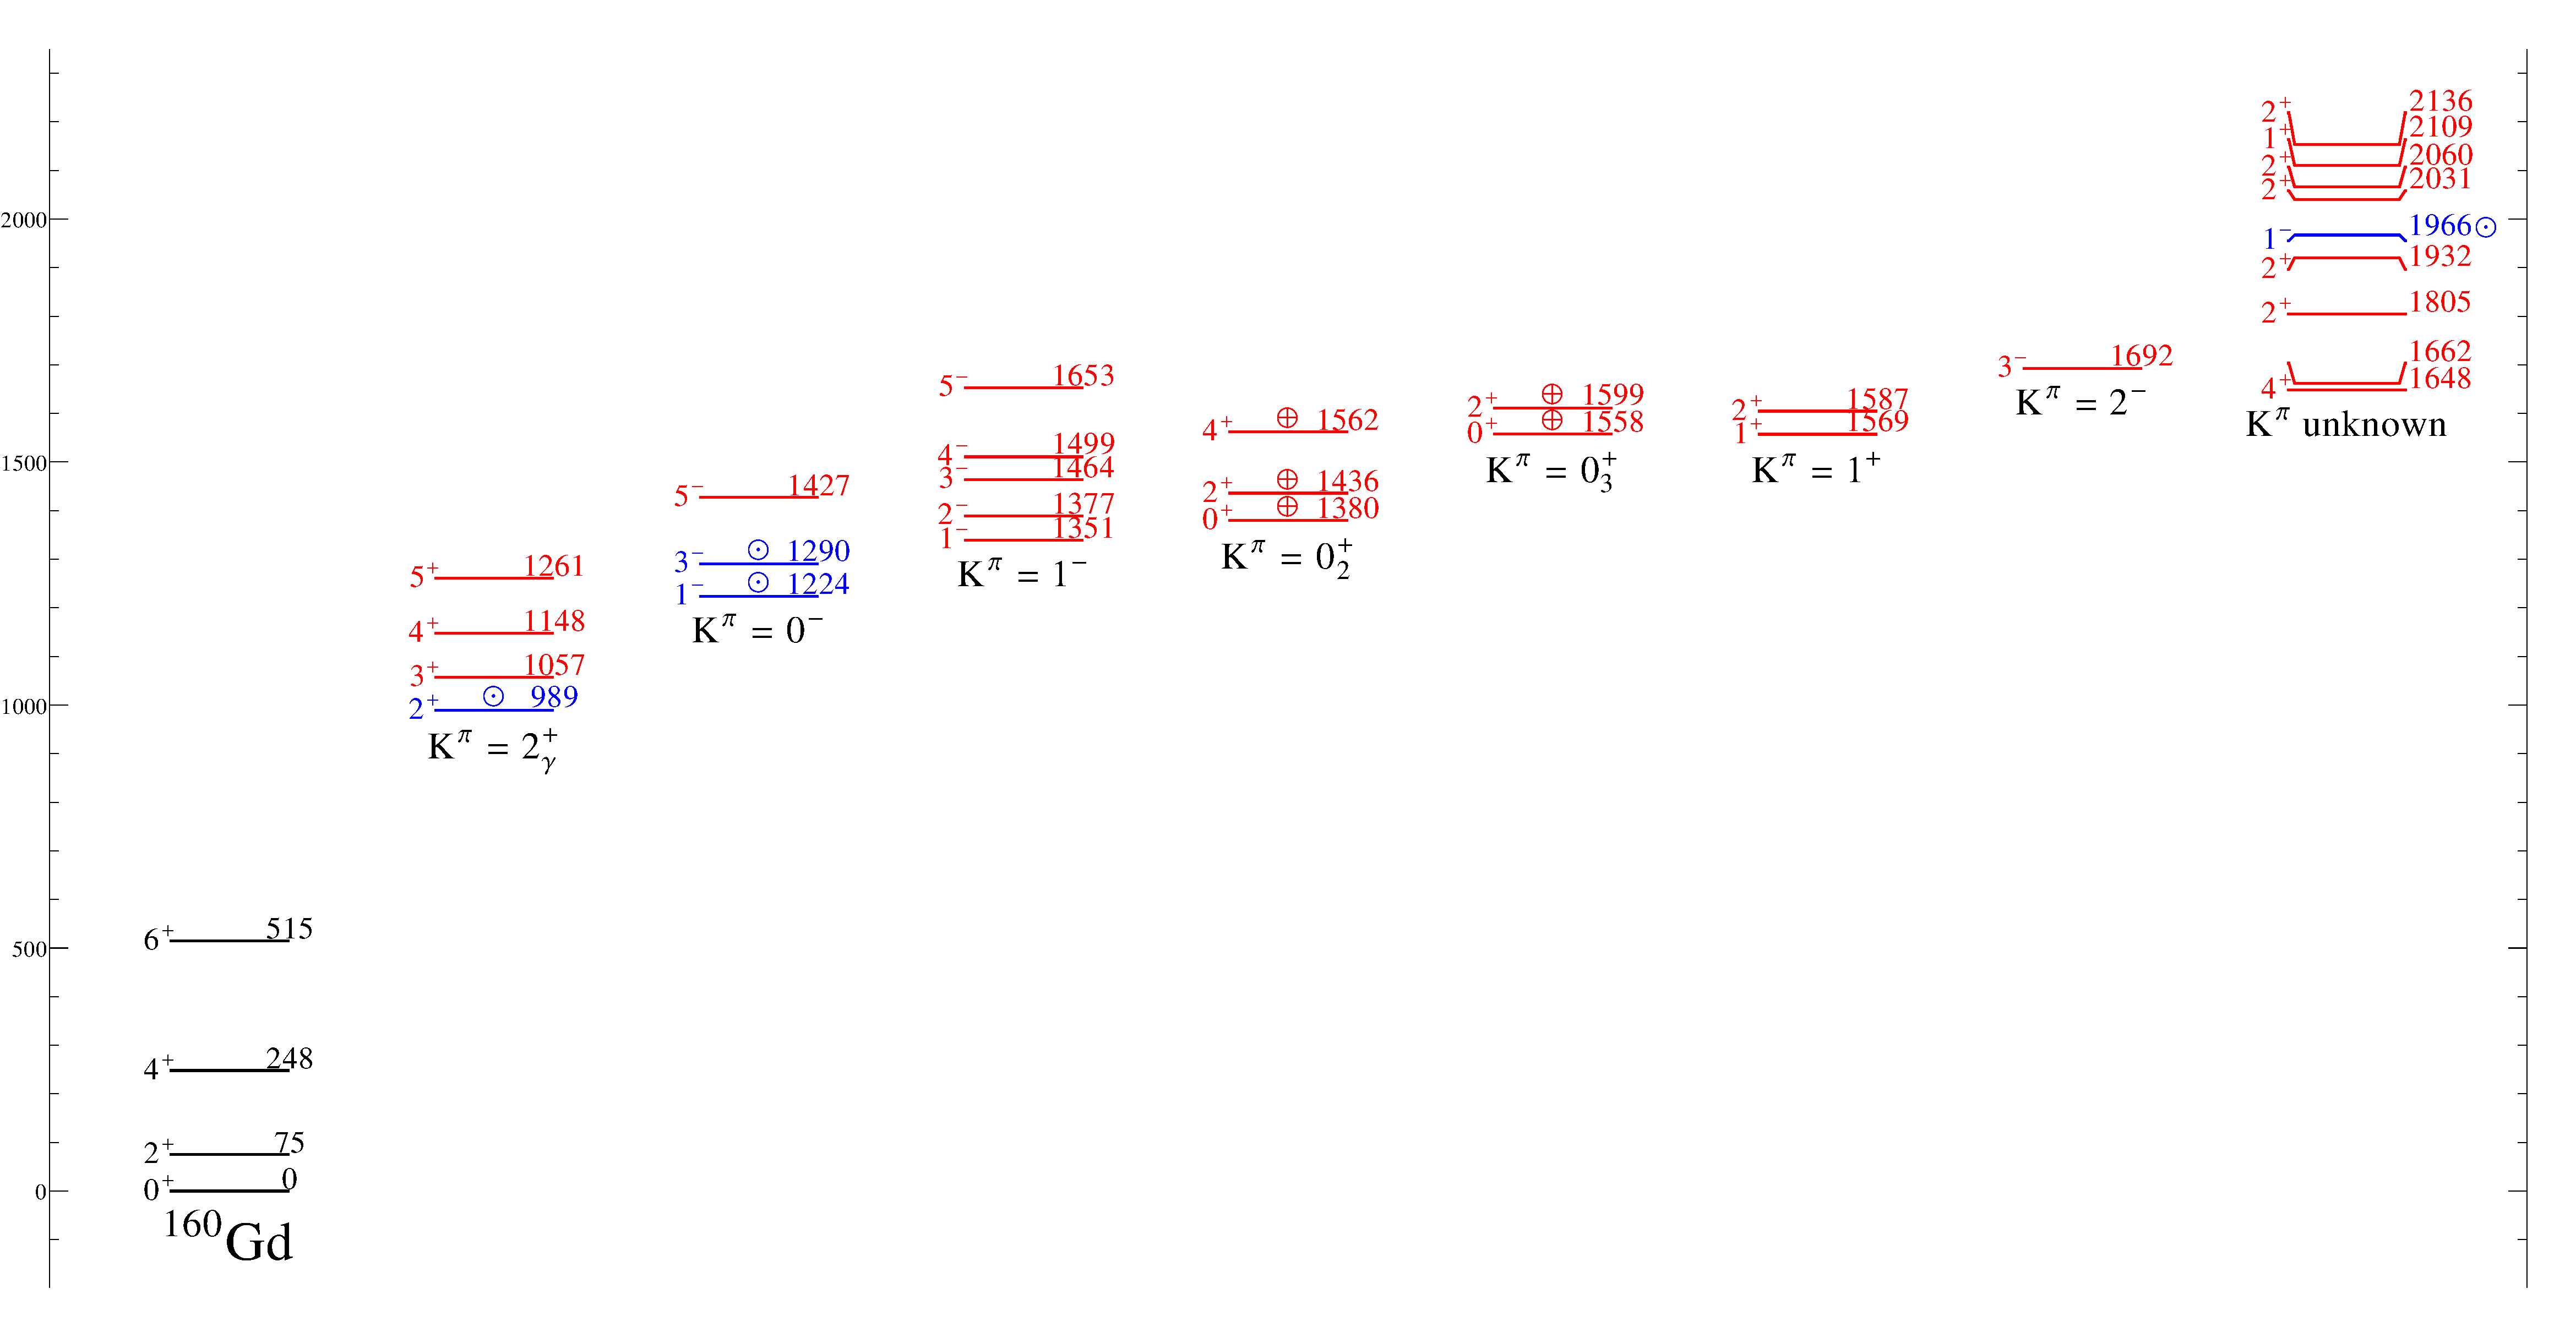
\includegraphics[height=0.85\textheight]{160Gd_All.pdf}
\caption{Level scheme for all level lifetimes measured in the $^{160}$Gd experiments, with confirmed band and spin assignments shown. Previously measured lifetimes are in blue, with newly presented lifetimes in red. Individual levels and bands will be discussed in following sections.
\label{fig:160Gd_All}}
\end{figure}
\end{center}
\end{landscape}

High resolution angular distribution measurements were performed by Govor in \cite{Govor_160Gd_2009} and provide us with an overall benchmark for our measurements, and as a whole, our reported $\gamma$-ray intensities, angular distribution coefficients, and multipole mixing ratios are found to be in good agreement with the work. One key contrasted element in our work with the Govor paper is the use of monoenergetic neutrons for DSAM-INS rather than the continuum energies of reactor neutrons to extract the lifetimes in addition to any decay information ($\gamma$-ray energies, multipole mixing fractions, etc). A visual representation of the all the measured lifetimes in $^{160}$Gd is shown in Figure \ref{fig:160Gd_viz_lifetimes}, with literature values in black and new lifetimes in red (corresponding to lifetime extracted from the E$_n$=1.5~MeV dataset), green for 2.0~MeV neutrons, and blue for the final dataset using 2.8~MeV neutrons bombardement. %This figure also serves to show which bombarding neutron energies are used to extract level lifetimes (to minimize the inflation outlined as an example in Figure \ref{fig:lifetime_inflation}).

\begin{figure}[h!]
\begin{center}
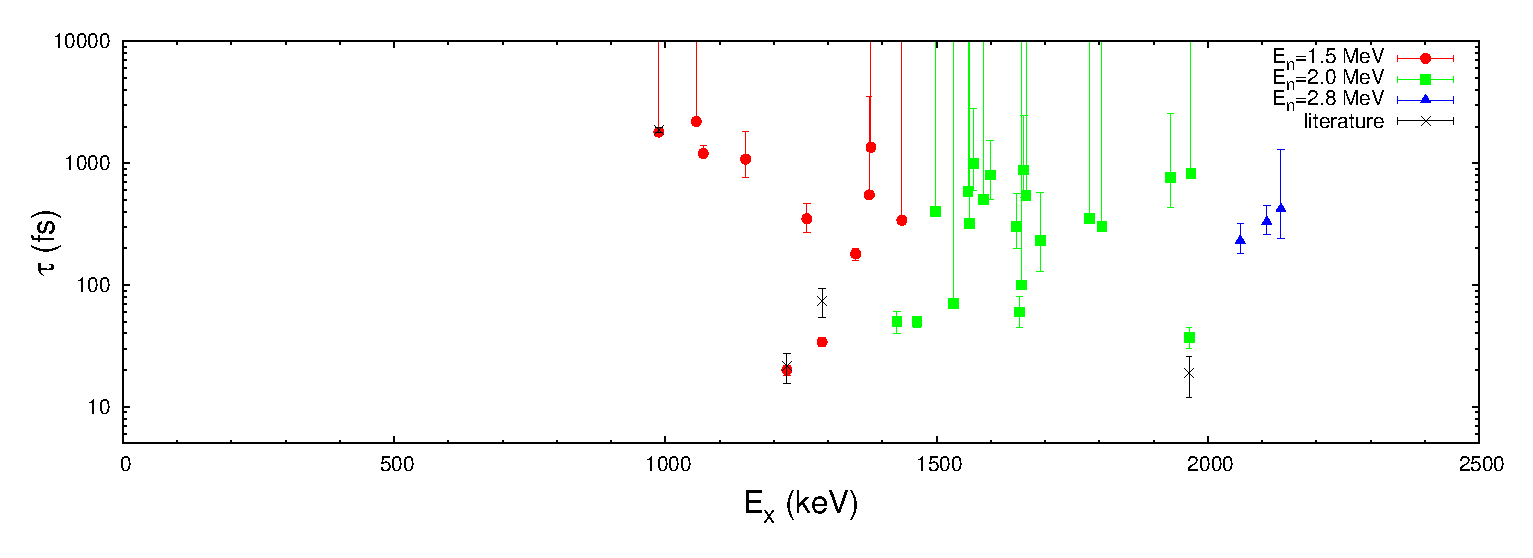
\includegraphics[width=0.95\textwidth]{160Gd_viz_lifetimes.eps}
\caption{Visual representation of all measured lifetimes with respect to literature values (in blue). Each separate color outlines the specific regimes ($<$1.5~MeV, 1.5~-~2.0~MeV, and $>$2.0~MeV excitation energy) of energies studied in the $^{160}$Gd angular distributions. \label{fig:160Gd_viz_lifetimes}}
\end{center}
\end{figure}

An example of the E$_n$=2.0~MeV angular distribution singles-spectrum for $^{160}$Gd(n,n$^\prime\gamma$) can be seen in Figure \ref{fig:160Gd_200_spectrum} with select peaks labeled for reference.

\begin{figure}[h!]
\begin{center}
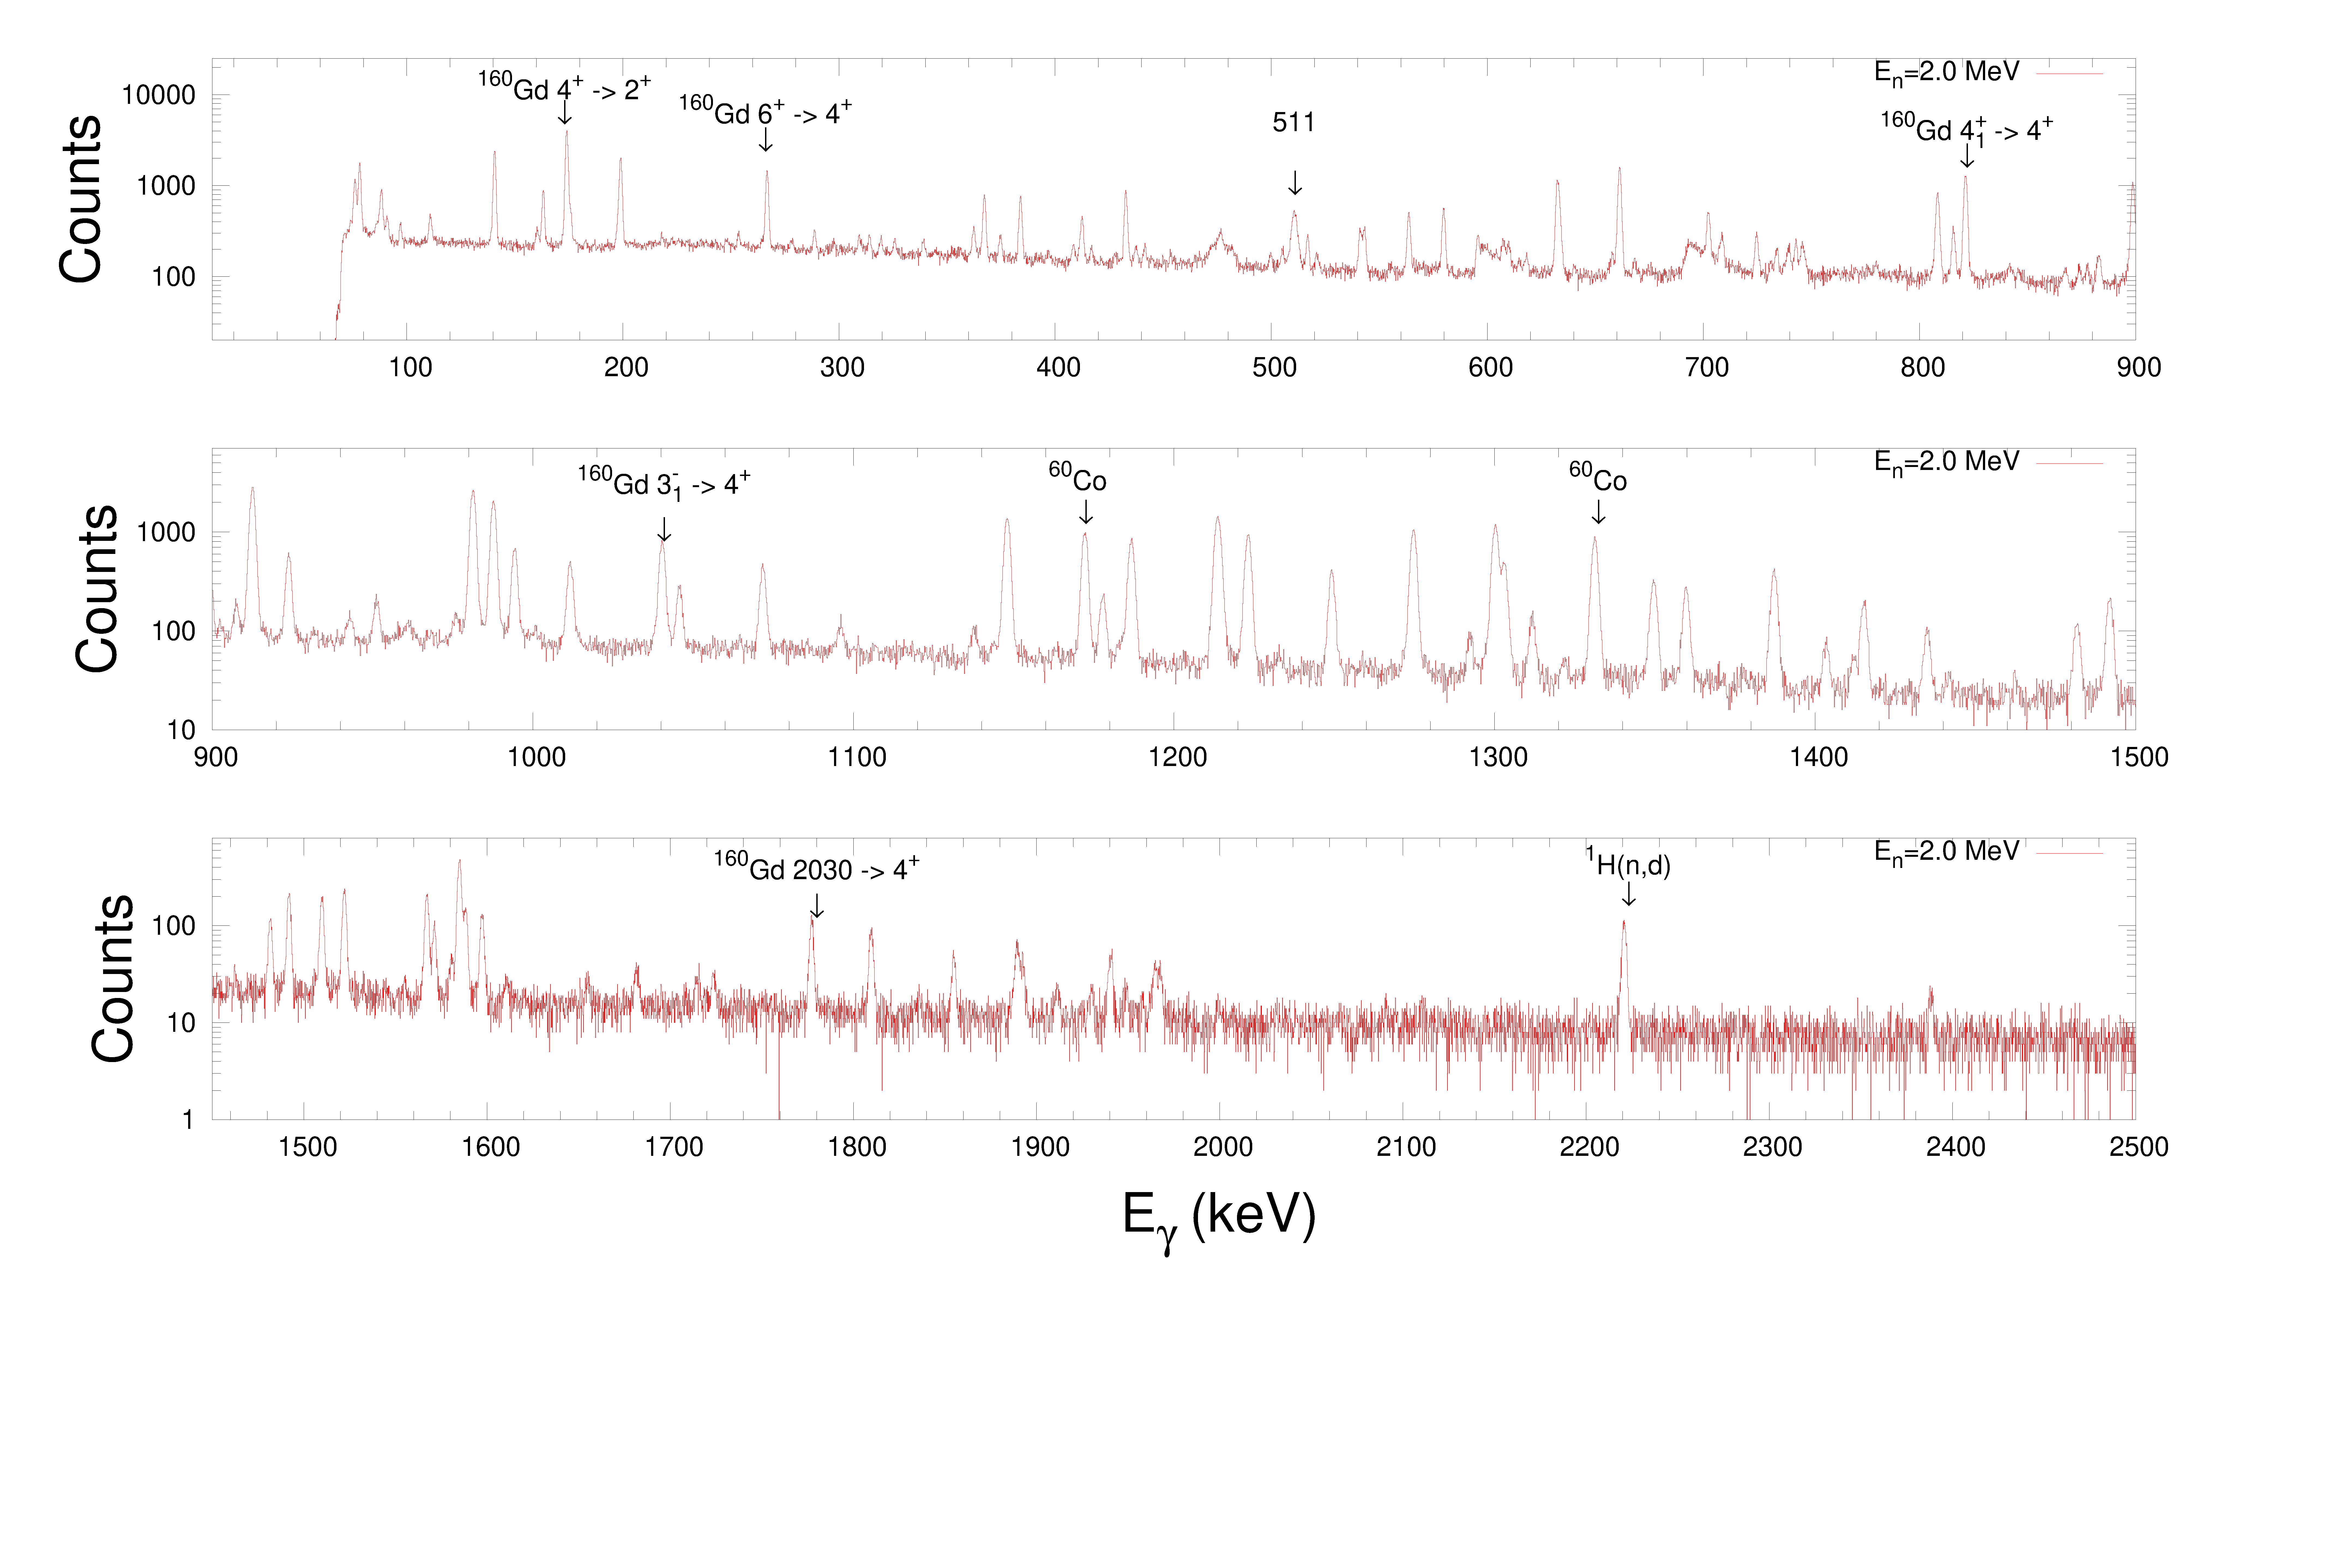
\includegraphics[width=0.95\textwidth]{160Gd_200_spectra.eps}
\caption{Singles spectra from the $\theta_{lab}$=90$^\circ$ and E$_n$=2.0~MeV angular distributions of $^{160}$Gd. \label{fig:160Gd_200_spectrum}}
\end{center}
\end{figure}

% visualization and preface to results (overview)
\subsection{Lifetimes of 0$^+$ States}
%lifetimes of 0$^+$ states overview
The tabulation of lifetimes for the 0$^+$ bands in $^{160}$Gd is given in Table \ref{tab:160Gd_0s_all}. In many cases, F($\tau$) values for $\gamma$ rays were small, and as such, we are only able to extract lower limits for the level lifetimes. Further refinement of the level lifetime for the E$_{\rm x}$=1599~keV state was provided in [TBA REF], where any negative (and consequently impossible) F($\tau$) attenuation factors were removed from the weighted average for the level lifetime.

\begin{landscape}
\begin{table}[h!]
\begin{center}
\caption{K$^\pi$=0$^+$ BANDS: $^{160}$GD  \label{tab:160Gd_0s_all}}
% \makebox[\textwidth]{
\begin{tabular}{cccccccccc}
E$_{level}$ (keV) & E$_\gamma$ (keV) & J$^\pi_{K^\pi_i}$ & J$^\pi_{K^\pi_f}$ & $\tau$ (fs) & BR & Mult. &  B(E2) (W.u.) & B(E1) (mW.u.)\\
\hline
\hline
1379.70 (7) & 1304.46 (5) & 0$^+_{0^+_2}$ & 2$^+_{0^+_1}$ & $>$1350 & 1.000 & E2 & $<$3.10 & \\
1436.47 (4) & 1187.81 (5) & 2$^+_{0^+_2}$ & 4$^+_{0^+_1}$ & $>$340  & 0.667 & E2 & $<$13.1 & \\
            & 1361.05 (6) & 2$^+_{0^+_2}$ & 2$^+_{0^+_1}$ &         & 0.243 & E2/M1$^{[a]}$ & $<$2.42 & \\
            & 1436.34 (6) & 2$^+_{0^+_2}$ & 0$^+_{0^+_1}$ &         & 0.090 & E2 & $<$0.68 & \\
1561.59 (6) & 1046.67 (6) & 4$^+_{0^+_2}$ & 6$^+_{0^+_1}$ & $>$320  & 0.572 & E2 & $<$22 & \\
            & 1313.03 (6) & 4$^+_{0^+_2}$ & 4$^+_{0^+_1}$ &         & 0.428 & E2/M1$^{[b]}$ & $<$0.4 & \\   
            \hline
1558.30 (7) & 1483.06 (6) & 0$^+_{0^+_3}$ & 2$^+_{0^+_1}$ & $>$590  & 1.000 & E2 & $<$3.74 & \\
1599.00 (4) &  309.32 (6) & 2$^+_{0^+_3}$ & 3$^-_{0^-_1}$ & 800$^{+730}_{-300}$  & 0.037 & E1 &  & 0.34$^{+0.13}_{-0.31}$ \\
            &  374.78 (6) & 2$^+_{0^+_3}$ & 1$^-_{0^-_1}$ &              & 0.062 & E1 &  & 0.32$^{+0.12}_{-0.29}$ \\
            &  541.53 (6) & 2$^+_{0^+_3}$ & 3$^+_{2^+_\gamma}$ &         & 0.154 & E2/M1$^{[c]}$ & 41$^{+16}_{-37}$ & \\     
            & 1523.59 (6) & 2$^+_{0^+_3}$ & 2$^+_{0^+_1}$ &              & 0.418 & E2/M1$^{[d]}$ & 0.34$^{+0.68}_{-0.32}$ & \\
            & 1598.85 (6) & 2$^+_{0^+_3}$ & 0$^+_{0^+_1}$ &              & 0.329 & E2 & 0.41$^{+0.15}_{-0.37}$ & \\
            \hline

\end{tabular}\\ \vspace{10pt} \end{center}
% \begin{center}
Lifetimes of excited 0$^+$ bands in $^{160}$Gd, with experimentally determined B(E2) in W.u and B(E1) in mW.u.
$^{[a]}\delta$=0.00$^{+0.08}_{-0.08}$, $^{[b]}\delta$=0.28$^{+0.34}_{-0.12}$, $^{[c]}\delta$=-5.57$^{+1.91}_{-5.00}$, $^{[d]}\delta$=-1.04$^{+0.72}_{-2.10}$,%\\
1~W.u.(E2)=5.16E-7~e$^2$b$^2$, 1~mW.u.(E1)=1.90~e$^2$b\\
% \end{center}
\end{table}
\end{landscape}

\subsection{Lifetimes of 2$^+_\gamma$ Band}
%we have measured lifetimes in the gamma band yada yada
We have measured lifetimes for the 4 lowest-lying members of the K$^\pi$=2$^+$ band in $^{160}$Gd in our campaign of experiments. Throughout the rare-earth region of nuclei, the 2$^+$ band lifetimes are generally well known and fall in the near-picosecond lifetime range \cite{McGowan_BE2_1981,Burke_hexadecapole1994,PhysRevC.54.679,JAMMARI_1988}. Due to the sensitive range of DSAM, these near-picosecond lifetimes manifest as lower-limits due to the shallow F($\tau$) values observed in our experiments; however, we obtain well-defined values for the 4$^+$ and 5$^+$ members of the 2$^+$ band via some well-defined energy shifts, all shown in Table \ref{tab:160Gd_gamma}.

\begin{table}[h!]
\begin{center}
\caption{K$^\pi$=2$^+$ BAND: $^{160}$GD \label{tab:160Gd_gamma}}

\begin{tabular}{ccccccccc}
E$_{level}$ (keV) & E$_\gamma$ (keV) & J$^\pi_{K^\pi_i}$ & J$^\pi_{K^\pi_f}$ & $\tau$ (fs) & BR & Mult. &  B(E2) (W.u.) \\
\hline
\hline
988.72 (6)  & 913.43 (5) & 2$^+_{2^+_\gamma}$ & 2$^+_{0^+_{gs}}$ & $>$1800 & 0.530 & E2/M1$^{[a]}$ & $<$1.2\\%$^{+0.22}_{-0.18}$  \\ 
            & 988.68 (5) & 2$^+_{2^+_\gamma}$ & 0$^+_{0^+_{gs}}$ &         & 0.470 & E2         & $<$4.1\\%$^{+0.2}_{-0.2}$  \\ 

1057.42 (6) & 809.06 (5) & 3$^+_{2^+_\gamma}$ & 4$^+_{0^+_{gs}}$ & $>$2200 & 0.171 & E2/M1$^{[b]}$ & $<$0.04  \\ 
            & 982.28 (5) & 3$^+_{2^+_\gamma}$ & 2$^+_{0^+_{gs}}$ &         & 0.829 & E2/M1$^{[c]}$ & $<$6.5  \\ 

1148.15 (7) & 899.59 (5)  & 4$^+_{2^+_\gamma}$ & 4$^+_{0^+_{gs}}$ & 1080$^{+730}_{-320}$ & 0.631 & E2/M1$^{[d]}$ & 16$^{+5}_{-10}$  \\ 
            & 1072.85 (5) & 4$^+_{2^+_\gamma}$ & 2$^+_{0^+_{gs}}$ &                      & 0.369 & E2         & 3.8$^{+2.6}_{-1.1}$  \\ 

1261.24 (9) & 746.34 (5)  & 5$^+_{2^+_\gamma}$ & 6$^+_{0^+_{gs}}$ & 350$^{+120}_{-80}$ & 0.164 & E2/M1$^{[e]}$ & 31$^{+7}_{-11}$  \\ 
            & 1012.65 (5) & 5$^+_{2^+_\gamma}$ & 4$^+_{0^+_{gs}}$ &                    & 0.836 & E2/M1$^{[f]}$ & 35$^{+8}_{-12}$  \\ 
            \hline    
\end{tabular}\\ \vspace{10pt} \end{center}
Lifetimes of K$^\pi$=2$^+_\gamma$ band in $^{160}$Gd, with experimentally determined B(E2) in W.u. and multipole mixing fractions $\delta$ taken from the E$_n$=1.5~MeV angular distributions.
$^{[a]}\delta$=-0.45$^{+0.04}_{-0.05}$, $^{[b]}\delta$=0.11$^{+0.03}_{-0.03}$, $^{[c]}\delta$=47$^{+18}_{-10}$, $^{[d]}\delta$=21$^{+21}_{-7}$, $^{[e]}\delta$=8$^{+13}_{-4}$, $^{[f]}\delta$=15$^{+17}_{-6}$\\
1~W.u.(E2)=5.16E-7~e$^2$b$^2$\\
% \end{center}
\end{table}

\subsection{Lifetimes of Negative Parity Bands}

Population of the K$^\pi$=0$^-$ bands in rare-earth nuclei is abundant \cite{Zilges_K0dipole}, showing up as some of the strongest peaks in our $\gamma$-singles spectra, with a very low angular momentum transfer needed to populate the states ($\Delta$K=0). Typically, since the lowest-lying negative parity states are collective octupole vibrations on top of the deformed ground state, the mean lifetimes of these states are comparatively short, acting as a practical benchmark for lifetimes measurable by DSAM-INS. All three level lifetimes from the K$^\pi$=0$^-$ band in $^{160}$Gd were measured from the inelastic scatter of 1.5~MeV neutrons, using the five $\gamma$-rays listed in Table \ref{tab:160Gd_negparity}.

Similar to the K$^\pi$=0$^-$ band, the K$^\pi$=1$^-$ band in $^{160}$Gd is richly populated in our (n,n$^\prime\gamma$) experiments, with four band members (1$^-$,2$^-$,3$^-$,4$^-$) all proposed by Govor in another (n,n$^\prime\gamma$) study \cite{Govor_160Gd_2009} using continuum energy reactor neutrons in contrast to our monoenergetic probe. Of the specific lifetimes measured from the Doppler shifting $\gamma$-rays, we observe a weak decay from the 2$^-$ state to the $\gamma$-vibrational band; this branching ratio is so weak that it \textit{could} be misplaced, however, the threshold of the de-excitation in our excitation function does not place it leaving any other level. The resulting lifetime from the 1301~keV $\gamma$ ray is only a lower-limit due to the shallow F($\tau$) value.

Grigoriev \cite{Grigoriev2012} places a K$^\pi$=2$^-$ assignment on the band with the E$_{\rm x}$=1691 \& 1782~keV members that was tentatively either a 2$^-$ or 3$^-$. We adopt this 2$^-$ assignment from our observed $\gamma$-decay channels, even without the measurement or observation of the 2$^-$ bandhead in our data.

\begin{table}[h!]    
\begin{center}
\caption{NEGATIVE PARITY BANDS: $^{160}$GD \label{tab:160Gd_negparity}}
                            
% \makebox[\textwidth]{                           
\begin{tabular}{ccccccccc}
E$_{level}$ (keV) & E$_\gamma$ (keV) & J$^\pi_{K^\pi_i}$ & J$^\pi_{K^\pi_f}$ & $\tau$ (fs) & BR & Mult. &   B(E1) (mW.u.)\\
\hline
\hline
1224.33 (6)  & 1149.12 (5) & 1$^-_{0^-_1}$ & 2$^+_{0^+_1}$ & 20$^{+2}_{-2}$   & 0.597 & E1   & 6.5$^{+0.6}_{-0.6}$ &\\
             & 1224.38 (5) & 1$^-_{0^-_1}$ & 0$^+_{0^+_1}$ &                  & 0.403 & E1   & 3.6$^{+0.4}_{-0.4}$ &\\
1289.90 (7)  & 1041.37 (5) & 3$^-_{0^-_1}$ & 4$^+_{0^+_1}$ & 34$^{+3}_{-3}$   & 0.353 & E1   & 3.0$^{+0.3}_{-0.3}$ &\\
             & 1214.79 (5) & 3$^-_{0^-_1}$ & 2$^+_{0^+_1}$ &                  & 0.647 & E1   & 3.5$^{+0.3}_{-0.3}$ &\\
1427.40 (12) & 1214.79 (5) & 5$^-_{0^-_1}$ & 4$^+_{0^+_1}$ & 50$^{+10}_{-10}$ & 1.000 & E1   & 4.0$^{+0.8}_{-0.8}$ &\\
\hline
1351.30 (6)  & 1276.06 (5) & 1$^-_{1^-_1}$ & 2$^+_{0^+_1}$ & 180$^{+20}_{-20}$      & 0.833 & E1   & 0.74$^{+0.08}_{-0.08}$ &\\
             & 1351.30 (5) & 1$^-_{1^-_1}$ & 0$^+_{0^+_1}$ &                        & 0.167 & E1   & 0.12$^{+0.01}_{-0.01}$ &\\
1376.70 (8)  &  319.38 (6) & 2$^-_{1^-_1}$ & 3$^+_{2^+_\gamma}$ & $>$550            & 0.017 & E1   & $<$0.18 &\\
             & 1301.46 (5) & 2$^-_{1^-_1}$ & 2$^+_{0^+_1}$ &                        & 0.982 & E1   & $<$0.27 &\\
1464.00 (10) & 1388.75 (5) & 3$^-_{1^-_1}$ & 2$^+_{0^+_1}$ & 50$^{+5}_{-5}$         & 1.000 & E1  & 2.5$^{+0.2}_{-0.2}$ &\\
1498.94 (10) & 1250.39 (5) & 4$^-_{1^-_1}$ & 4$^+_{0^+_1}$ & $>$400                 & 1.000 & E1  & $<$0.41  &\\

\hline
1691.68 (7)  &  543.45 (6) & 3$^-_{2^-_1}$ & 4$^+_{2^+_\gamma}$ & 230$^{+350}_{-100}$ & 0.226 & E1   & 2$^{+1}_{-3}$ &\\
             &  634.56 (6) & 3$^-_{2^-_1}$ & 3$^+_{2^+_\gamma}$ &                     & 0.370 & E1   & 2.1$^{+0.9}_{-3.2}$ &\\
             &  702.84 (6) & 3$^-_{2^-_1}$ & 2$^+_{2^+_\gamma}$ &                     & 0.372 & E1   & 1.5$^{+0.7}_{-2.3}$ &\\
             & 1442.93 (8) & 3$^-_{2^-_1}$ & 4$^+_{0^+_1}$ &                          & 0.032 & E1   & 0.01$^{+0.01}_{-0.02}$ &\\
1782.67 (10) &  521.53 (8) & 4$^-_{2^-_1}$ & 5$^+_{2^+_\gamma}$ & $>$350              & 0.208 & E1   & $<$2.0 &\\
             &  725.19 (6) & 4$^-_{2^-_1}$ & 3$^+_{2^+_\gamma}$ &                     & 0.792 & E1   & $<$1.4 &\\
\end{tabular}\\ \vspace{10pt}
\end{center}
Lifetimes of excited negative parity bands in $^{160}$Gd, with experimentally determined B(E1) in mW.u. 
% 1~mW.u.(E1)=1.90~e$^2$b\\
\end{table}

\subsection{Lifetimes of Positive Parity Bands}
In addition to the measurement of lifetimes of K=0,2 and negative parity bands, we are also able to populate the vast majority of states below J=5. Lifetimes of positive parity bands were measured in $^{160}$Gd, namely of the K$^\pi$=4$^+$ and 1$^+$ bands. The full tabulation of measured lifetimes can be found in Table \ref{tab:160Gd_posparity}.


\begin{table}[h!]
\begin{center}
\caption{POSITIVE PARITY (K$^\pi$=4$^+$/1$^+$ BANDS): $^{160}$GD \label{tab:160Gd_posparity}}
\begin{tabular}{ccccccccc}
E$_{level}$ (keV) & E$_\gamma$ (keV) & J$^\pi_{K^\pi_i}$ & J$^\pi_{K^\pi_f}$ & $\tau$ (fs) & BR & Mult. &  B($\pi\ell$) \\
\hline
\hline
1070.57 (7) & 555.45 (8) & 4$^+_{4^+_1}$ & 6$^+_{0^+_1}$ & $>$1200  & 0.010 & E2            & $<$2.4  \\
            & 822.06 (5) & 4$^+_{4^+_1}$ & 4$^+_{0^+_1}$ &          & 0.603 & E2/M1$^{[a]}$ & $<$7.2  \\
            & 995.30 (5) & 4$^+_{4^+_1}$ & 2$^+_{0^+_1}$ &          & 0.387 & E2            & $<$5.2  \\
            \hline
1568.77 (6) & 217.51 (6)  & 1$^+_{1^+_1}$ & 1$^-_{1^-_1}$ & 1000$^{+1800}_{-400}$  & 0.030 & E1             & 0.97$^{+0.7}_{-1.8}$ \\
            & 580.20 (6)  & 1$^+_{1^+_1}$ & 2$^+_{2^+_\gamma}$ &                   & 0.305 & E2/M1$^{[b]}$  & 5.3$^{+6.7}_{-13}$  \\
            & 1493.40 (6) & 1$^+_{1^+_1}$ & 2$^+_{0^+_1}$ &                        & 0.323 & E2/M1$^{[c]}$  & 0.44$^{+0.23}_{-0.88}$  \\
            & 1568.70 (6) & 1$^+_{1^+_1}$ & 0$^+_{0^+_1}$ &                        & 0.342 & E2/M1$^{[*]}$  & 0.56$^{+0.22}_{-1.01}$  \\
1586.61 (12) & 1511.36 (6) & 2$^+_{1^+_1}$ & 2$^+_{0^+_1}$& $>$500                 & 1.000 & E2            & $<$4.01  \\
1665.16 (8) & 288.57 (6)  & 3$^+_{1^+_1}$ & 2$^-_{1^-_1}$ & $>$540                 & 0.115 & E1            & $<$2.9 \\
            & 1416.59 (6) & 3$^+_{1^+_1}$ & 4$^+_{0^+_1}$ &                        & 0.462 & E2/M1$^{[d]}$ & $<$0.73  \\
            & 1589.81 (6) & 3$^+_{1^+_1}$ & 2$^+_{0^+_1}$ &                        & 0.423 & E2/M1$^{[e]}$ & $<$0.95  \\
            \hline

\end{tabular}\\ \vspace{10pt}
\end{center}
% \begin{center}
Lifetimes of excited positive parity bands in $^{160}$Gd, with experimentally determined B(E2) in W.u and  B(E1) in mW.u. \\
$^{[a]}\delta$=-0.72$^{+0.06}_{-0.05}$, $^{[b]}\delta$=0.28$^{+0.25}_{-0.18}$, $^{[c]}\delta$=1.34$^{+1.6}_{-0.6}$, $^{[d]}\delta$=0.67$^{+0.11}_{-0.08}$, $^{[e]}\delta$=-1.87$^{+0.18}_{-0.18}$\\
$^{[*]}$ Full E2 strength is reported (no $\delta$ was calculated)\\
1~W.u.(E2)=5.16E-7~e$^2$b$^2$, 1~mW.u.(E1)=1.90~e$^2$b\\
% \end{center}
\end{table}

\subsection{Lifetimes of States with No K$^\pi$ Assignment}
The remaining lifetimes of states with no rotational band assignment are tabulated in Table \ref{tab:160Gd_Kunknown} and presented with deduced transition probabilities in Figure \ref{fig:160Gd_Kunknown}. We place stringent limits on the spin and parity of these states by confirming all de-excitations exhibit the same qualitative shape in the excitation functions, and by examining the Legendre polynomial coefficients to ascertain changes in angular momentum. In many cases, this is easily done if the radiation pattern is strongly E2 or E1; for mixed-multipolarity $\gamma$ rays, comparison to the {\tt CINDY} code is possible to restrict possible spin assignments. Generally, {\tt CINDY} is used as a baseline, rough assignment, as the statistical model behaves much better at lower mass nuclei, such as $^{76}$Ge or $^{106}$Pd \cite{Crider_76Ge_cindy,Peters2016_Pdshapecoex}, where the density of states above the pairing gap is smaller, and as such are tentative assignments placed by our (n,n$^\prime\gamma$) study.

% \begin{landscape}
\begin{table}[h!]
\begin{center}
\caption{OTHER LEVELS: $^{160}$GD \label{tab:160Gd_Kunknown}}

\begin{tabular}{ccccccccc}
E$_{level}$ (keV) & E$_\gamma$ (keV) & J$^\pi_{K^\pi_i}$ & J$^\pi_{K^\pi_f}$ & $\tau$ (fs) & BR & Mult. &  B($\pi\ell$) \\
\hline
\hline
1805.13 (9) & 734.50 (6)  & 2$^+_{[\Upsilon]}$ & 4$^+_{4^+_1}$ & $>$300   & 0.307 & E2                    & $<$76  \\
            & 816.46 (6)  & 2$^+_{[\Upsilon]}$ & 2$^+_{2^+_1}$ &          & 0.693 & E2/M1$^{[a]}$         & $<$37  \\\hline
1931.96 (7) &  874.51 (6) & 2$^+_{[\Upsilon]}$ & 3$^+_{2^+_1}$ & 760$^{+1800}_{-330}$  & 0.197 & E2/M1$^{[b]}$         & 8$^{+3.5}_{-19}$  \\
            & 1683.45 (7) & 2$^+_{[\Upsilon]}$ & 4$^+_{0^+_1}$ &                       & 0.206 & E2                    & 0.32$^{+0.14}_{-0.75}$  \\
            & 1856.65 (6) & 2$^+_{[\Upsilon]}$ & 2$^+_{0^+_1}$ &                       & 0.454 & E2/M1$^{[c]}$         & 0.20$^{+0.17}_{-0.47}$  \\
            & 1932.00 (7) & 2$^+_{[\Upsilon]}$ & 0$^+_{0^+_1}$ &                       & 0.143 & E2                    & 0.11$^{+0.05}_{-0.26}$  \\\hline
1966.66 (10)& 1891.33 (6) & 1$^+_{[\Upsilon]}$ & 2$^+_{0^+_1}$ & 37$^{+8}_{-7}$  & 0.637 & E1         & 0.84 $^{+0.28}_{-0.21}$  \\
            & 1966.97 (13)& 1$^+_{[\Upsilon]}$ & 0$^+_{0^+_1}$ &                 & 0.363 & E1         & 0.43 $^{+0.16}_{-0.11}$  \\\hline
1969.84 (9) & 1894.50 (6) & 2$^+_{[\Upsilon]}$ & 2$^+_{0^+_1}$ & $>$830   & 0.582 & E2/M1$^{[*]}$         & $<$0.45  \\
            & 1969.93 (7) & 2$^+_{[\Upsilon]}$ & 0$^+_{0^+_1}$ &          & 0.418 & E2                    & $<$0.27  \\\hline
2030.90 (9) & 1782.14 (6) & 2$^+_{[\Upsilon]}$ & 4$^+_{0^+_1}$ & $>$255   & 0.139 & E2/M1$^{[*]}$         & $<$0.47  \\
            & 1955.93 (7) & 2$^+_{[\Upsilon]}$ & 2$^+_{0^+_1}$ &          & 0.861 & E2                    & $<$1.84  \\\hline
2060.43 (11)& 2060.42 (6) & 2$^+_{[\Upsilon]}$ & 6$^+_{0^+_1}$ & 230$^{+90}_{-50}$  & 1.000 & E2         & 1.82 $^{+0.40}_{-0.71}$  \\\hline
2109.32 (7) & 1051.87 (6) & 1$^+_{[\Upsilon]}$ & 3$^+_{2^+_1}$ & 330$^{+120}_{-70}$   & 0.170 & E2                     & 6.23 $^{+1.34}_{-2.28}$ \\
            & 1119.71 (13)& 1$^+_{[\Upsilon]}$ & 2$^+_{2^+_1}$ &                     & 0.208 & E2/M1$^{[*]}$          & 5.57 $^{+1.21}_{-2.04}$ \\
            & 2034.26 (6) & 1$^+_{[\Upsilon]}$ & 2$^+_{0^+_1}$ &                      & 0.359 & E2/M1$^{[*]}$          & 0.49 $^{+0.10}_{-0.18}$ \\
            & 2109.31 (6) & 1$^+_{[\Upsilon]}$ & 0$^+_{0^+_1}$ &                      & 0.263 & E2/M1$^{[*]}$          & 0.30 $^{+0.06}_{-0.11}$ \\ \hline
2135.76 (13)& 2135.74 (7) & 2$^+_{[\Upsilon]}$ & 0$^+_{0^+_1}$ & 420$^{+880}_{-180}$  & 1.000 & E2         & 0.83 $^{+0.36}_{-1.75}$   \\

\end{tabular}\\ \vspace{10pt}
\end{center}
% \begin{center}
Lifetimes of excited states in $^{160}$Gd that have no K band assignment, with experimentally determined B(E2) in W.u and  B(E1) in mW.u. \\
$^{[a]}\delta$=-0.76$^{+0.10}_{-0.13}$, $^{[b]}\delta$=-3.3$^{+1.1}_{-2.4}$,  $^{[c]}\delta$=0.92$^{+0.41}_{-0.64}$\\
$^{[*]}$ Full E2 strength is reported (no $\delta$ was calculated)\\
1~W.u.(E2)=5.16E-7~e$^2$b$^2$, 1~mW.u.(E1)=1.90~e$^2$b\\
$[\Upsilon]$: No rotational K$^\pi$ band assignment given in literature.
% \end{center}
\end{table}
% \end{landscape}

% \subsection{Other (Intensity info)}

  \section{$^{162}$Dy Results}

$^{162}$Dy, one of the most studied nuclei on the chart of nuclides, with over 24 different reactions and probes (from electron capture, stripping/pickup (t,p)/(p,t) reactions, neutron capture, ($\alpha$,2n) reactions, and ($^3$He,$\alpha$) reactions, to name a few) which have been implemented to extract information on the structure of $^{162}$Dy \cite{Aprahamian200642}. Several previous (n,n$^\prime\gamma$) campaigns were carried out to measure level lifetimes of the isovector M1 scissors mode in $^{162}$Dy (\cite{Yates_162nnp1995}), as well as a series of precision angular distribution measurements by Govor \textit{et.~al} (\cite{Govor_162Dy2002}) to extract multipole mixing fractions and $\gamma$-ray intensities. Analogous to the $^{160}$Gd case study, the angular distributions carried out by Govor act as a complimentary guide and benchmark for our measurements. While the initial and chief goal is to measure the lifetimes of 0$^+$ excitations and low-lying negative parity states, we are also able to populate and measure the lifetimes of the vast majority of low spin (J$<$5) states under the bombarding neutron energy threshold. The full result of all measured lifetimes in the $^{162}$Dy experimental campaign (\S \ref{sec:Dy_exp}) is displayed in the level scheme in Figure \ref{fig:162Dy_All}.

% \begin{center}
% \begin{figure}[h!]
% 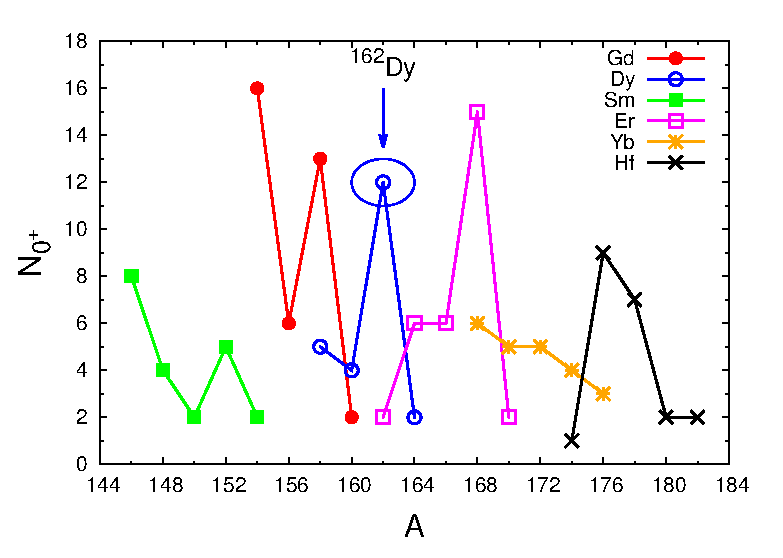
\includegraphics[width=0.90\textwidth]{Gd_Dy_0s_Number.eps}
% \caption{Schematic of the total number of 0$^+$ excitations among several deformed rare-earth nuclei (Sm, Gd, Dy, Er, Yb, and Hf), with emphasis drawn to $^{162}$Dy in a blue circle. \label{fig:RE_0s}}
% \end{figure}
% \end{center}
\begin{landscape}
\begin{figure}[h!]
\begin{center}
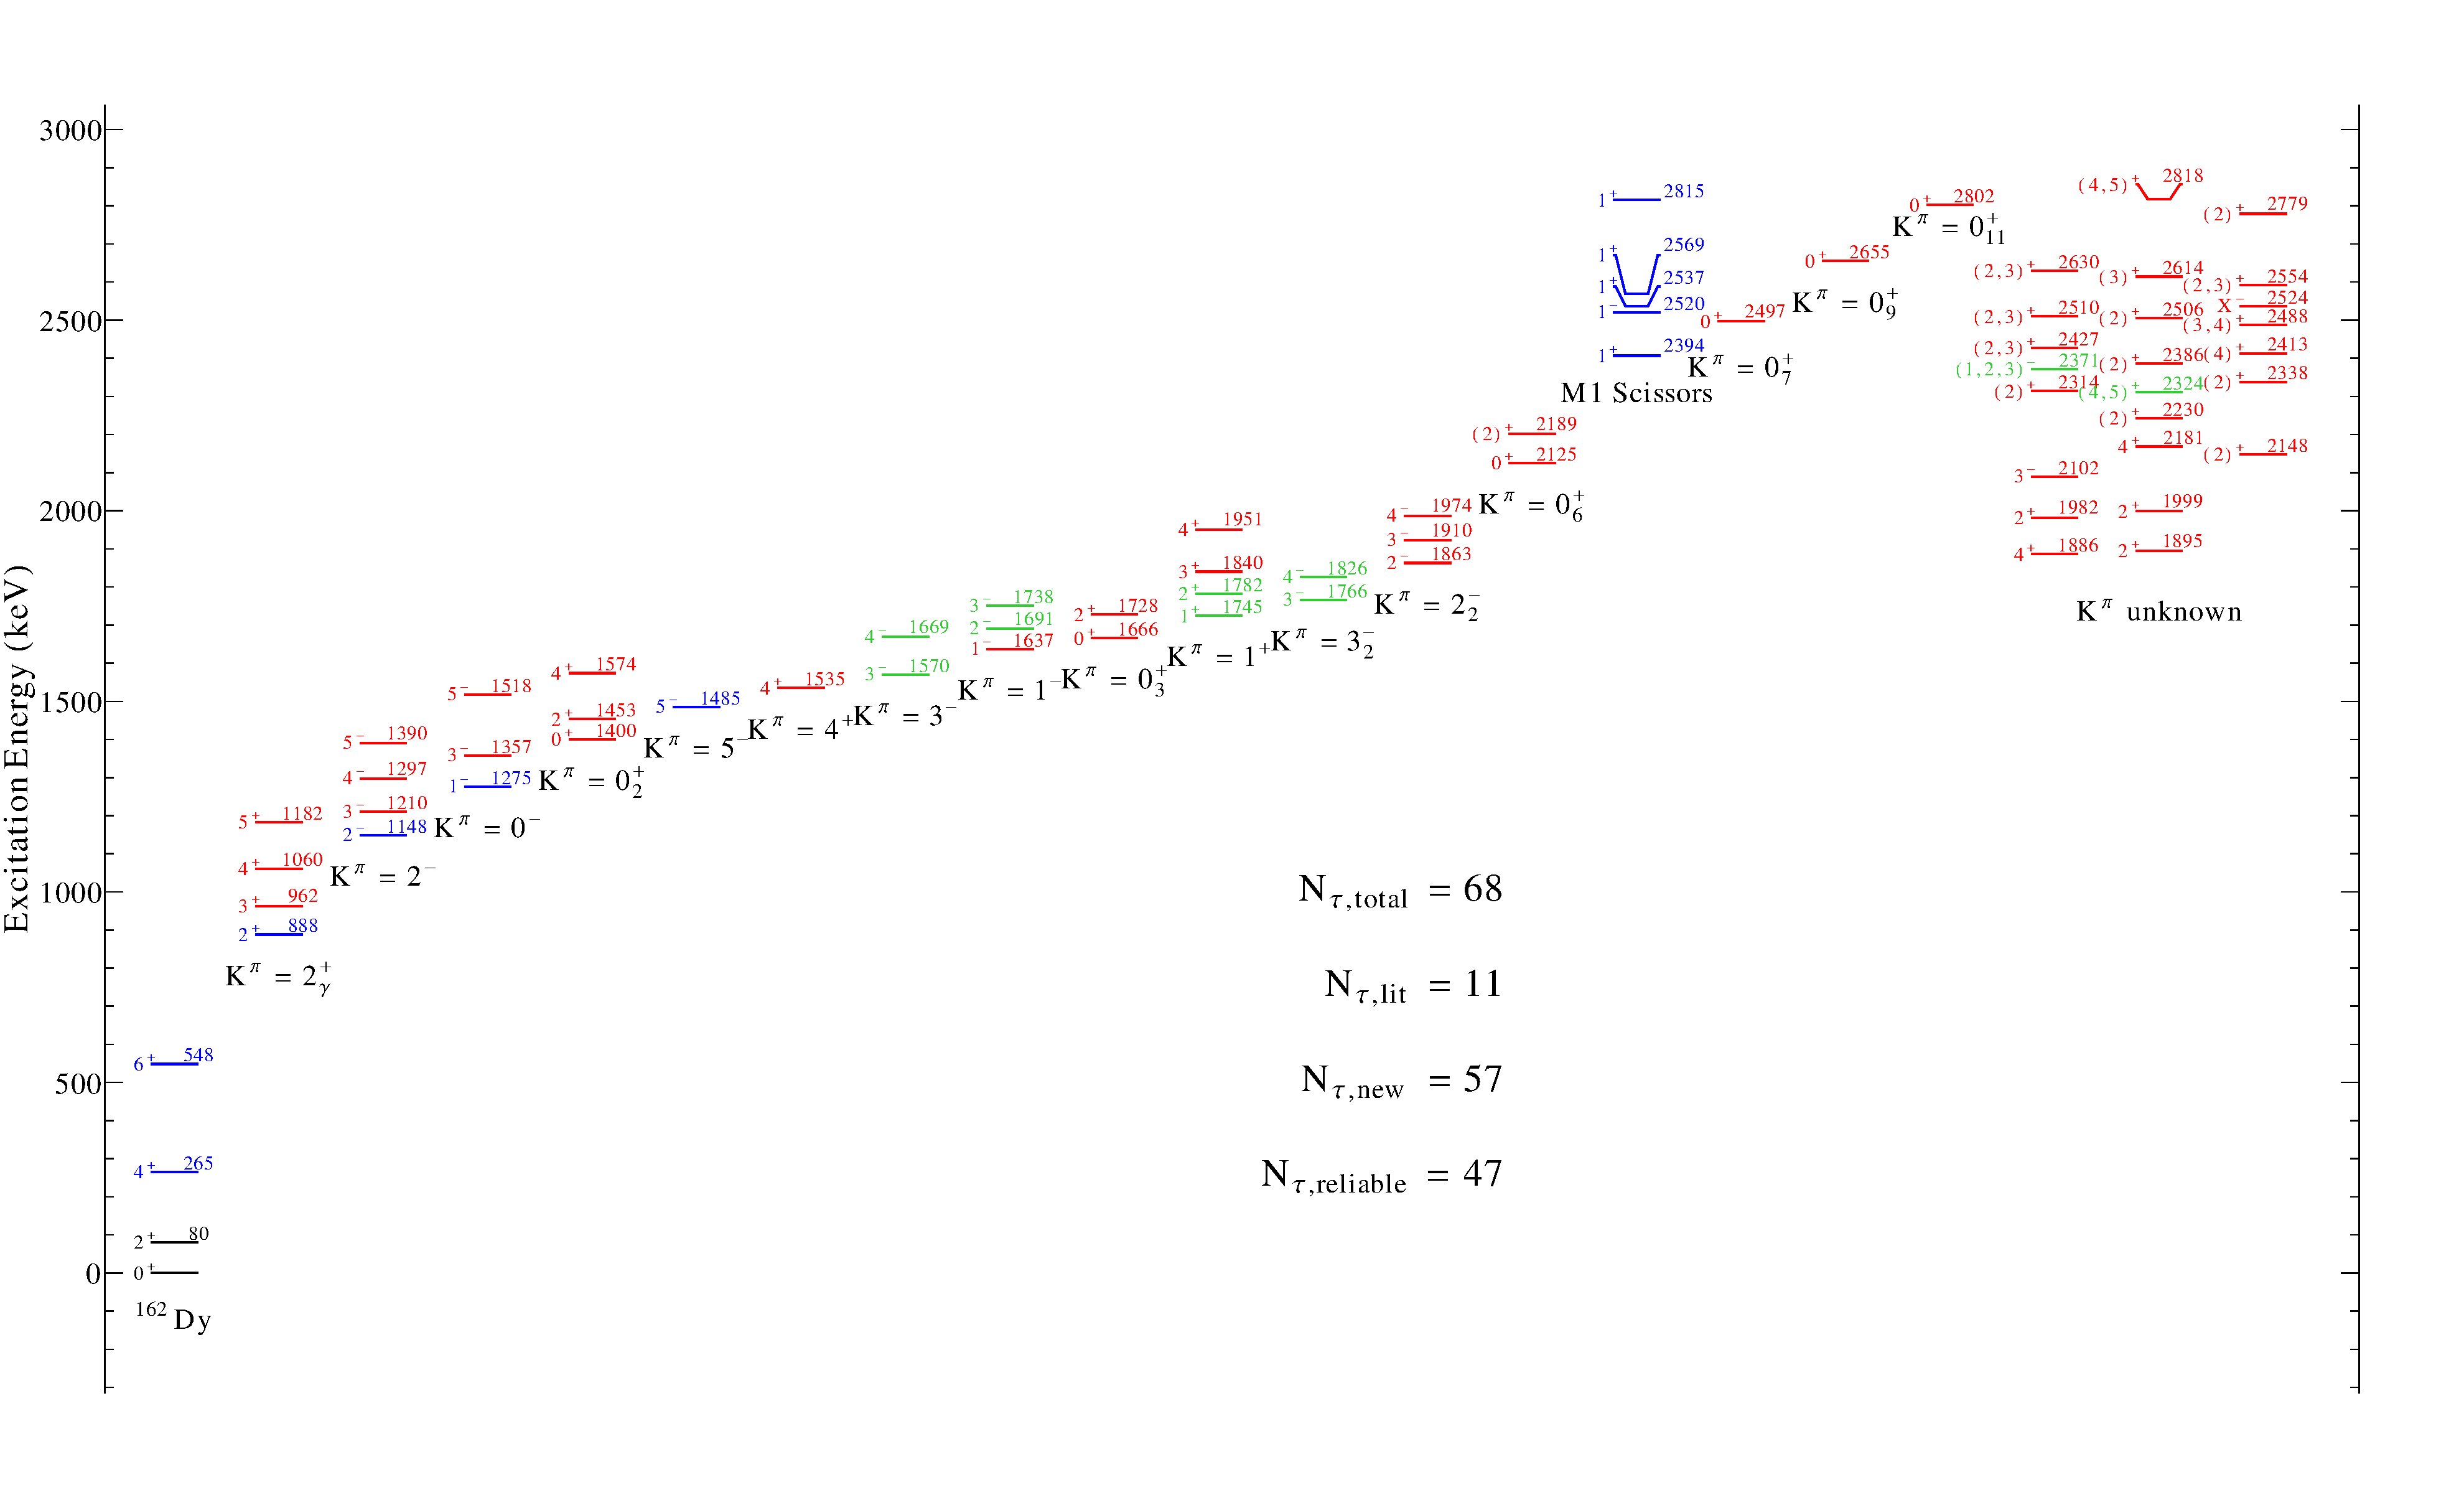
\includegraphics[height=0.8\textheight]{figures/162Dy_All.pdf}
\caption{Level scheme for all level lifetimes measured in the $^{162}$Dy experiments, with confirmed band and spin assignments shown. Previously measured lifetimes are in blue, with newly presented lifetimes in red, levels in green constitute an unreliable lifetime measurement from our data, where F($\tau$)$<$0 or is consistent with zero. 
\label{fig:162Dy_All}}
\end{center}
\end{figure}

\end{landscape}

In Figure \ref{fig:162Dy_All}, levels colored blue are pre-existing lifetimes in literature, where the levels in red are newly presented lifetime measurements in this work. Due to the limitations of DSAM outlined in \S \ref{sec:AD_Ft}, cases where F($\tau$) is strictly less than zero or consistent with 0 within 1$\sigma$, unreliable lifetimes are colored green. Again, it must be reiterated that while these lifetimes do not have previously measured literature values, our (n,n$^\prime\gamma$) lifetimes should not be trusted as a good measurement. Other techniques must be implemented to fully measure the lifetime of these states (Coulomb Excitation, RDDM plunger method, etc). Excitations are placed into bands where available, along with the well-measured and studied isovector M1 scissors mode lifetimes at $\sim$2.4~MeV that results in J$^\pi$=1$^{\pm}$ excitations \cite{Margraf_gg'NRF_1995, WESSELBORG198822,Yates_162nnp1995}. In total, we observed 108 discrete $\gamma$-rays to measure sixty eight (68) lifetimes, fifty seven (57) of which were measured for the first time. Of the newly measured lifetimes, however, only forty seven (47) are considered reliable from our measurement of Doppler energy shifted $\gamma$ rays. These measured lifetimes were extracted from the three angular distribution measurements (E$_n$=1.6, 2.2, \& 3.1~MeV), with three effective ranges of lifetime sensitivity, in the hopes of limiting any lifetime feeding from higher levels and bombarding neutron energy. Visually, the ranges of lifetimes reported can be seen in Figure \ref{fig:162Dy_viz_lifetimes}, where we have a comparison of the presented lifetimes (and corresponding errors) in to literature lifetimes in the three separate ranges of lifetime sensitivity (excitation energies of $<$1.6~MeV in red, 1.6~-~2.2~MeV in green, and 2.2~MeV~-~3.1~MeV in blue). 


\begin{table}[h!]
\begin{center}
\caption{LITERATURE LIFETIME COMPARISON: $^{162}$DY \label{tab:lifetimes_comparison}}
% \makebox[\textwidth]{
\begin{tabular}{c|c|c}
E$_{lev}$ (keV) & $\tau_{(n,n^\prime\gamma)}$ (fs) & $\tau_{lit}$ (fs) \\
\hline
\hline
265  & $>$1500[$\dagger$]      & 0.190E6 (7) [$\oplus$] \\
548  & $>$960[$\dagger$]       & 26.5E3 (14) [$\oplus$] \\
888  & $>$3700                 & 2840 (3) [$\oplus$] \\
1148 & 2100$^{+7200}_{-1200}$  & 0.30E6 (6) [$\ominus$]\\
1275 & 120$^{+10}_{-10}$   & 28.8 (6) [$\ddagger$][$\oplus$]\\
1485 & 400$^{+210}_{-140}$ & 2.76E6 (16) [$\ddagger$][$\otimes$]\\
2394 & 14$^{+13}_{-11}$    & 16$^{+10}_{-10}$ [$\Omega$]\\
2520 & 110$^{+30}_{-20}$   & 11$^{+9}_{-9}$ [$\Omega$]\\
2537 & 460$^{+160}_{-120}$ & 141$^{+30}_{-30}$ [$\Omega$]\\
2569 & 90$^{+30}_{-20}$    & 56$^{+6}_{-6}$ [$\Omega$]\\
2815 & 200$^{+130}_{-60}$  & 56$^{+19}_{-19}$ [$\Omega$] \\
\end{tabular}\\ \vspace{10pt}
\end{center}
Comparison of lifetimes measured in the campaign of $^{162}$Dy(n,n$^\prime\gamma$) experiments with literature lifetimes.
[$\dagger$]: Measured lifetime not reliable (F($\tau$) within 1$\sigma$ of 0) - resulting lifetimes fall well outside the range of DSAM.
[$\ddagger$]: Lifetime called into question in this work. 
[$\ominus$]: from $^{162}$Tb $\beta^-$ decay \cite{PhysRev.166.1227}.
[$\otimes$]: from $^{162}$Ho $\varepsilon$-decay \cite{Honig_5minus1969}. 
[$\oplus$]: from B(E2)$\uparrow$ via Coul. Ex \cite{GROTDAL1968385}. 
[$\Omega$]: from ($\gamma$,$\gamma^\prime$) \cite{Margraf_gg'NRF_1995} and (n,n$^\prime\gamma$) \cite{Yates_162nnp1995}
% \end{center}
\end{table}

% \begin{figure}[h!]
% \begin{center}
% \includegraphics[width=0.95\textwidth]{162Dy_viz_lifetimes.eps}
% \caption{Visual representation of all measured lifetimes with respect to literature values (in black). Each separate color outlines the specific regimes ($<$1.6~MeV (in red), 1.6~-~2.2~MeV (in green), and 2.2~MeV~-~3.1~MeV (in blue) excitation energy) of energies studied in the $^{162}$Dy angular distributions. \label{fig:162Dy_lifetimes}}
% \end{center}
% \end{figure}

The discrepancies from the literature lifetimes are clearly visible in Figure \ref{fig:162Dy_viz_lifetimes}, where we can attribute slight inflation of the lifetimes as a result of either feeding from higher-lying states, or from the bombarding neutron energy effects mentioned at the beginning of \S \ref{sec:lifetime_inflation}. We can make the justification that our lifetimes agree reasonably with literature because the accuracy of measurement is roughly on the same order of magnitude for every sensitive range of lifetimes measured, with scattered cases of good agreement. In other words, the lifetimes measured at intermediate energies ($\sim$900~keV, $\sim$1850~keV, and $\sim$2400~keV) are inflated by the same proportional amount for each bombarding neutron energy. Further discrepancies in our measured lifetimes to those in literature stem from the differences in measurement techniques (DSAM-INS versus deduction of lifetimes via direct B(E1/M1)$\uparrow$). For example, the weighted average of the F($\tau$) values for multi-channel decays out of a state can result in a lower average F($\tau$) if only one $\gamma$-ray decay is used in the determination of the lifetime, resulting in a longer lifetime. 

\begin{figure}[h!]
\begin{center}
\includegraphics[width=0.999\textwidth]{figures/162Dy_viz_lifetimes.eps}
\caption{All measured lifetimes in $^{162}$Dy (in femtoseconds) plotted as a function of excitation energy in keV. Data points in red are extracted from the E$_n$=1.6~MeV angular distributions, points in green correspond to lifetimes extracted from the 2.2~MeV angular distributions, and blue points are lifetimes from the 3.1~MeV dataset. (color online) \label{fig:162Dy_viz_lifetimes}}
\end{center}
\end{figure}

An example of the E$_n$=2.2~MeV angular distribution singles-spectrum for $^{162}$Dy(n,n$^\prime\gamma$) can be seen in Figure \ref{fig:162Dy_220_spectrum} with select peaks labeled for reference.

\begin{figure}[h!]
\begin{center}
\includegraphics[width=0.95\textwidth]{figures/sample_spec_stacked_220.eps}
\caption{Singles spectra from the $\theta_{lab}$=90$^\circ$ and E$_n$=2.2~MeV angular distributions of $^{162}$Dy. \label{fig:162Dy_220_spectrum}}
\end{center}
\end{figure}

%visualization and preface to results (overview)
\subsection{Lifetimes of 0$^+$ States}
In stark contrast to the results of the $^{160}$Gd experiments (namely the lower limit lifetimes and existence of anisotropies in angular distributions), we are able to determine definite level lifetimes for the majority of 0$^+$ bands and confirm isotropic angular distributions from the $^{162}$Dy data. DSAM plots and angular distributions for the full 0$^+_i\rightarrow$2$^+_{g.s.}$ de-excitations are seen in Figures \ref{fig:162Dy_0s_FT} and \ref{fig:162Dy_0s_AD}, respectively. We also do not exclude any of the proposed 0$^+$ states from our observation of isotropic or anisotropies in the angular distributions similar to our $^{160}$Gd results.

\begin{figure}[h!]
\begin{center}
\includegraphics[width=0.95\textwidth]{figures/162Dy_0s_AD.pdf}
\caption{Angular distributions of 0$^+_i\rightarrow$2$^+_{g.s.}$ $\gamma$-rays observed in $^{162}$Dy, highlighting their isotropic nature (color online). \label{fig:162Dy_0s_AD}}
\end{center}
\end{figure}

\begin{figure}[h!]
\begin{center}
\includegraphics[width=0.95\textwidth]{figures/162Dy_0s_FT.pdf}
\caption{Doppler energy shifts of 0$^+_i\rightarrow$2$^+_{g.s.}$ $\gamma$-rays observed in $^{162}$Dy (color online). \label{fig:162Dy_0s_FT}}
\end{center}
\end{figure}

Lifetimes for six (6) of the eleven (11) confirmed and tentative excited 0$^+$ states \cite{Meyer_pt0_2006} were measured in the campaign of experiments (shown in Table \ref{tab:0s_comparison}). We have also measured lifetimes (including a few lower limits) of the five lowest-lying rotational members of the K$^\pi$=2$^+$ band, the bandheads of both K$^\pi$=4$^+$ bands, and a total of 52 other states in $^{162}$Dy. The absolute intensities of decays discussed in this work were extracted from the angular distributions and are shown in Table \ref{tab:162Dy_multiphonon_intensities}, with unobserved transition intensities taken from literature \cite{Aprahamian200642,Zamfir_162Dy0_1999,Wu_2minus_2001} to provide pertinent discussion later in this manuscript.


The full tabulation of $\gamma$ decays observed for the de-excitation of K$^\pi$=0$^+$ bands is shown in Table \ref{tab:162Dy_0s_all}, which includes experimentally measured lifetimes in femtoseconds, branching ratios, and $\gamma$-ray energies in keV. Mixed multipolarity de-excitations are assigned a multipole mixing fraction ($\delta_{mixing}$) from comparison of our gathered angular distributions to a statistical model calculation, performed with {\tt CINDY} \cite{SHELDON197399}. A level scheme outlining all observed decays from 0$^+$ bands to the ground state band is also shown in Figure \ref{fig:162Dy_0s_all}.

Lifetimes for the three lowest-lying rotational members of the 0$^+_2$ band were measured; the single, most intense $\gamma$ ray at 1319~keV was used to measure (a shallow) F($\tau$) to extract the lifetime from the E$_n$=1.6~MeV dataset. The weighted average of F($\tau$) from both the 1187 \& 1372~keV $\gamma$ ray is used to measure the lifetime of the 2$^+$ state. Only the 1308~keV de-excitation contributes to the lifetime of the 4$^+$ state at E$_{\rm x}$=1574~keV, as the 1025~keV transition exhibits a negative F($\tau$) value.

We have measured the lifetime of the bandhead and 2$^+$ member of the 0$^+_3$ band at E$_{\rm x}$=1666~keV, with good lifetime resolution extracted from the E$_n$=2.2~MeV dataset. The single 1585~keV transition from the bandhead to the ground state yields a 3000$^{+4800}_{-1300}$~fs lifetime, while only the 1647 and 1728~keV $\gamma$ rays offer contributions to the 2$^+$ lifetime of 1800$^{+880}_{-430}$~fs, as the decay at 1462~keV is coincident with a background line, making that particular F($\tau$) unreliable. Large uncertainties exist for the bandhead of this 0$^+$ band due to the natural limits of lifetimes measurable with DSAM; this large error stems from the uncertainties on the measured F($\tau$) value.

We adopt the placement \cite{BERZINS1995413} of the (2$^+$) state at 2189~keV as the 2$^+$ rotational band member of the 0$^+_6$ band at E$_{\rm x}$=2128~keV, and have measured lifetimes for these two states from the single-channel decays of 2109 \& 2047~keV, respectively. The lifetime of the bandhead was found to be 2300$^{+1500}_{-860}$~fs, and 530$^{+220}_{-160}$~fs for the 2$^+$ member.

The seventh and ninth 0$^+$ states decay via full energy de-excitations to the ground state at E$_\gamma$=2417 \& 2575~keV, respectively. These corresponding lifetimes extracted from the E$_n$=3.1~MeV dataset are 270$^{+110}_{-60}$~fs for the 0$^+$ state at 2497~keV, and 210$^{+300}_{-100}$~fs at 2655~keV. 

Due to the isotropic radiation observed for the 2721~keV $\gamma$-ray that depopulates the (0$^+_{11}$) state at 2802~keV, we support the assignment of this state as a 0$^+$ excitation, where further mentions of this state are considered as a confirmed 0$^+$ state. The Doppler shift from this 2721~keV decay gives us our shortest 0$^+$ lifetime of 90$^{+110}_{-60}$~fs.

\begin{landscape}
\begin{center}
% \begin{table}[h!]
\begin{longtable}{cllcccllll}
% \begin{center}
\caption{K$^\pi$=0$^+$ BANDS: $^{162}$DY \label{tab:162Dy_0s_all}}\\

% \resizebox{1.15\textwidth}{!}{
% \begin{tabular}{cllcccllll}
K$^\pi$                         & E$_{level}$ (keV) & E$_\gamma$ (keV) & J$^\pi_{K^\pi_i}$ & J$^\pi_{K^\pi_f}$ & F($\tau$)$_{av}$ & $\tau$ (fs)                       & BR             & $\pi\ell$         & B($\pi\ell$) (W.u.) \\ \hline \hline \endfirsthead
\caption[]{K$^\pi$=0$^+$ BANDS: $^{162}$DY}{Continued}\\
K$^\pi$                         & E$_{level}$ (keV) & E$_\gamma$ (keV) & J$^\pi_{K^\pi_i}$ & J$^\pi_{K^\pi_f}$ & F($\tau$)$_{av}$ & $\tau$ (fs)                       & BR             & $\pi\ell$         & B($\pi\ell$) (W.u.) \\ \hline \hline \endhead
\underline{K$^\pi$=0$^+_2$:}    & 1400.29(36)  & 512.0(2)                   & 0$^+_{0^+_2}$    & 2$^+_{2^+_1}$ &0.031$\pm$0.038& $>$2100$^{[\vartheta]}$                 & $^{[\dagger]}$ & E2                & ($<$16) \\
                                &              & 1319.60(51)                & 0$^+_{0^+_2}$    & 2$^+_{0^+_1}$ &&                                                     & 1.000          & E2                & $<$1.9   \\
                                & 1453.50(30)  & 395.49 (10)                & 2$^+_{0^+_2}$    & 4$^+_{2^+_1}$ &0.042$\pm$0.026& 3400$^{+5600}_{-1300}$ $^{[\vartheta]}$ & $^{[\dagger]}$ & E2                & (2.7$^{+1.7}_{-1.7}$) \\
                                &              & 565.32 (12)                & 2$^+_{0^+_2}$    & 2$^+_{2^+_1}$ &&                                                     & $^{[\dagger]}$ & E2$^{[\ddagger]}$ & (0.9$^{+0.6}_{-0.6}$) \\
                                &              & 1187.81(51)                & 2$^+_{0^+_2}$    & 4$^+_{0^+_1}$ &&                                                     & 0.425(4)       & E2                & 0.8$^{+0.5}_{-0.5}$                         \\
                                &              & 1372.80(51)                & 2$^+_{0^+_2}$    & 2$^+_{0^+_1}$ &&                                                     & 0.575(4)       & E2/M1$^{[a\varsigma]}$& 0.3$^{+0.2}_{-0.2}$ \\  
                                & 1574.34(29)  & 513.31 (2)                 & 4$^+_{0^+_2}$    & 4$^+_{2^+_1}$ &0.043$\pm$0.031& $>$2000$^{[\varsigma]}$                  & $^{[\dagger]}$ & E2$^{[\ddagger]}$ & ($<$3.7) \\
                                &              & 611.23 (5)                 & 4$^+_{0^+_2}$    & 3$^+_{2^+_1}$ &&                                                     & $^{[\dagger]}$ & E2$^{[\ddagger]}$ & ($<$0.4) \\
                                &              & 686.15 (6)                 & 4$^+_{0^+_2}$    & 2$^+_{2^+_1}$ &&                                                     & $^{[\dagger]}$ & E2                & ($<$0.5) \\
                                &              & 1025.84(58)$^{[\oslash]}$  & 4$^+_{0^+_2}$    & 6$^+_{0^+_1}$ &&                                                     & 0.157(5)       & E2                & $<$1.1   \\
                                &              & 1308.65(51)                & 4$^+_{0^+_2}$    & 4$^+_{0^+_1}$ &&                                                     & 0.843(5)       & E2/M1$^{[b,\varsigma]}$& $<$0.8   \\          \hline
\underline{K$^\pi$=0$^+_3$:}    & 1666.01(33)  & 1585.35(51)                & 0$^+_{0^+_3}$    & 2$^+_{0^+_1}$ &0.051$\pm$0.033 & 3000$^{+4800}_{-1300}$ $^{[\varsigma]}$ & 1.000          & E2                & 0.5$^{+0.4}_{-0.3}$   \\
                                & 1728.31(20)  & 1462.70(51)$^{[\otimes]}$ & 2$^+_{0^+_3}$    & 4$^+_{0^+_1}$ &0.081$\pm$0.023& 1800$^{+880}_{-430}$ $^{[\varsigma]}$    &0.334(5)$^{[\star]}$ & E2           & 0.4$^{+0.1}_{-0.1}$ \\   
                                &              & 1647.64(51)                & 2$^+_{0^+_3}$    & 2$^+_{0^+_1}$ &&                                                     &0.407(5)        & E2/M1$^{[c,\varsigma]}$& 0.01$^{+0.01}_{-0.01}$ \\   
                                &              & 1728.29(53)                & 2$^+_{0^+_3}$    & 0$^+_{0^+_1}$ &&                                                     &0.259(4)        & E2                & 0.2$^{+0.1}_{-0.1}$  \\ \hline   
\underline{K$^\pi$=0$^+_6$:}    & 2128.02(33)  & 2047.34(61)                & 0$^+_{0^+_6}$    & 2$^+_{0^+_1}$ &0.071$\pm$0.031& 2300$^{+1500}_{-860}$ $^{[\varpi]}$ &1.000           & E2                & 0.2$^{+0.1}_{-0.1}$       \\  
                                & 2189.65(52)  & 2109.10(50)                & (2)$^+_{0^+_{6}}$& 2$^+_{0^+_1}$ &0.267$\pm$0.058& 530$^{+220}_{-160}$ $^{[\varpi]}$   &1.000           &(E2/M1)$^{[d,\varpi]}$    & 0.7$^{+0.3}_{-0.2}$   \\  \hline
\underline{K$^\pi$=0$^+_7$:}    & 2497.77(52)  & 2417.22(50)                & 0$^+_{0^+_7}$    & 2$^+_{0^+_1}$ &0.376$\pm$0.055& 270$^{+110}_{-60}$ $^{[\varpi]}$    &1.000           & E2                & 0.7$^{+0.2}_{-0.2}$     \\ \hline
\underline{K$^\pi$=0$^+_9$:}    & 2655.83(33)  & 2575.28(53)                & 0$^+_{0^+_9}$    & 2$^+_{0^+_1}$ &0.436$\pm$0.164& 210$^{+300}_{-100}$ $^{[\varpi]}$   &1.000           & E2                & 0.7$^{+0.6}_{-0.4}$       \\ \hline
\underline{K$^\pi$=0$^+_{11}$:} & 2802.04(61)  & 2721.48(55)                & 0$^+_{0^+_{11}}$ & 2$^+_{0^+_1}$ &0.653$\pm$0.200& 90$^{+110}_{-60}$ $^{[\varpi]}$     &1.000           & E2                & 1.2$^{+2.3}_{-0.6}$      \\ \hline
 
% \end{tabular}

\vspace{10pt}
\end{longtable}
\end{center}
Lifetimes of excited 0$^+$ bands in $^{162}$Dy, with calculated B(E2) in W.u., from our measured multipole mixing fractions, branching ratios, $\gamma$-ray energies, and lifetimes, all extracted from the angular distributions. B(E2) strengths in parentheses are calculated using literature intensities.\\
 $^{[a]}$: $\delta$=1.3$^{+0.2}_{-0.2}$,
 $^{[b]}$: $\delta$=0.93$^{+0.14}_{-0.15}$,
 $^{[c]}$: $\delta$=-0.22$^{+0.08}_{-0.08}$,
 $^{[d]}$: $\delta$=2.7$^{+1.8}_{-0.9}$\\
 $^{[\dagger]}$: Intensity information taken from \cite{Aprahamian200642,Zamfir_162Dy0_1999} ($\gamma$-ray not seen in this work),
 $^{[\ddagger]}$: Mixing information not available, full E2 strength reported,
 $^{[\oslash]}$: $\gamma$ ray not used in F($\tau$) calculation (F($\tau$)$<$0).\\
 $^{[\vartheta]}$: F($\tau$) or $\delta_{mixing}$ extracted from E$_n$=1.6~MeV angular distributions,
 $^{[\varsigma]}$: F($\tau$) or $\delta_{mixing}$ extracted from E$_n$=2.2~MeV angular distributions,
 $^{[\varpi]}$: F($\tau$) or $\delta_{mixing}$ extracted from E$_n$=3.1~MeV angular distributions,
 $^{[\otimes]}$: $\gamma$ ray coincident with background, not used in calculation of lifetime.\\
 1~W.u.=5.25E-7~e$^2$b$^2$
% \end{center}
% \end{table}
% \end{longtable}
% \end{center}
\end{landscape}

\subsection{Lifetimes of K$^\pi$=2$^+_\gamma$ and 4$^+$ Bands}

In the eight decays from the 2$^+$ band, two of the $\gamma$ rays (the 697~keV and 634~keV de-excitations) are not used in the calculation of the level lifetime, as they have Doppler shifts that correspond to an F($\tau$)$<$0. Lower limits for the lifetime are measured in several cases due to the inherent limitations of sensitive lifetimes DSAM can measure (up to a few picoseconds).


% \begin{table}[h!]
\begin{landscape}
\begin{center}
\begin{longtable}{cllcccllll}
\caption{K$^\pi$=2$^+$ AND 4$^+$ BANDS: $^{162}$DY \label{tab:162Dy_gamma_doublegamma}}\\ % \resizebox{1.15\textwidth}{!}{
% \begin{tabular}{cllcccllll}
K$^\pi$                           & E$_{level}$ (keV) & E$_\gamma$ (keV)     & J$^\pi_{K^\pi_i}$  & J$^\pi_{K^\pi_f}$  &F($\tau$)$_{av}$ & $\tau$ (fs)                        & BR        & $\pi\ell$     & B($\pi\ell$) (W.u.) \\ \hline \hline \endfirsthead
\caption[]{K$^\pi$=2$^+$ AND 4$^+$ BANDS: $^{162}$DY}{Continued}\\ % \resizebox{1.15\textwidth}{!}{
% \begin{tabular}{cllcccllll}
K$^\pi$                           & E$_{level}$ (keV) & E$_\gamma$ (keV)     & J$^\pi_{K^\pi_i}$  & J$^\pi_{K^\pi_f}$  &F($\tau$)$_{av}$ & $\tau$ (fs)                        & BR        & $\pi\ell$     & B($\pi\ell$) (W.u.) \\ \hline \hline \endhead
\underline{K$^\pi$=2$^+_\gamma$:} &  888.18(22) &  807.54(50)               & 2$^+_{2^+_\gamma}$ & 2$^+_{0^+_1}$ &0.022$\pm$0.018& $>$3700 $^{[\vartheta]}$                       & 0.524(3)            & E2/M1$^{[a,\vartheta]}$  & $<$1.1 \\
                                  &             &  888.18(50)               & 2$^+_{2^+_\gamma}$ & 0$^+_{0^+_1}$ &&                                                            & 0.476(3)            & E2                    & $<$3.6                            \\ 
                                  &  962.96(27) &  697.30(50)$^{[\oslash]}$ & 3$^+_{2^+_\gamma}$ & 4$^+_{0^+_1}$ &0.021$\pm$0.025& $>$3200 $^{[\vartheta]}$                       & 0.159(3)            & E2/M1$^{[b,\vartheta]}$  & $<$0.2    \\
                                  &             &  882.31(50)               & 3$^+_{2^+_\gamma}$ & 2$^+_{0^+_1}$ &&                                                            & 0.841(3)            & E2/M1$^{[c,\vartheta]}$  & $<$7.6                  \\ 
                                  & 1061.05(29) &  795.35(50)               & 4$^+_{2^+_\gamma}$ & 4$^+_{0^+_1}$ &0.047$\pm$0.030& 3200$^{+4800}_{-1300}$ $^{[\vartheta]}$        & 0.637(3)            & E2/M1$^{[d,\vartheta]}$  & 4.5$^{+2.7}_{-3.1}$ \\
                                  &             &  980.36(51)               & 4$^+_{2^+_\gamma}$ & 2$^+_{0^+_1}$ &&                                                            & 0.363(3)            & E2                    & 2.0$^{+1.3}_{-1.2}$             \\ 
                                  & 1182.88(26) &  634.24(61)               & 5$^+_{2^+_\gamma}$ & 6$^+_{0^+_1}$ &0.034$\pm$0.030& $>$2500 $^{[\varsigma]}$                        &0.239(5)             & E2/M1$^{[e,\vartheta]}$  & $<$14   \\
                                  &             &  917.18(51)               & 5$^+_{2^+_\gamma}$ & 4$^+_{0^+_1}$ &&                                                            &0.761(5)             & E2/M1$^{[f,\vartheta]}$  & $<$7.3   \\ \hline
\underline{K$^\pi$=4$^+_1$:}      & 1535.97(23) &  475.27(54)$^{[\otimes]}$& 4$^+_{4^+_1}$& 4$^+_{2^+_\gamma}$ &0.124$\pm$0.077& 1200$^{+2100}_{-450}$ $^{[\varsigma]}$           &0.186(10)$^{[\star]}$& E2/M1$^{[g,\varsigma]}$    & 44$^{+34}_{-40}$ (23$^{+18}_{-21}$)       \\
                                  &             &  572.96(50)               & 4$^+_{4^+_1}$& 3$^+_{2^+_\gamma}$ &&                                                             &0.317(6)             & E2/M1$^{[h,\varsigma]}$    & 66$^{+42}_{-40}$ (98$^{+63}_{-59}$)       \\
                                  &             &  647.61(50)$^{[\oslash]}$ & 4$^+_{4^+_1}$& 2$^+_{2^+_\gamma}$ &&                                                             &0.497(7)             & E2                     & 57$^{+34}_{-36}$ (120$^{+74}_{-78}$)       \\ \hline
\underline{K$^\pi$=4$^+_2$:}      & 2180.69(53) &  1217.73(58)              & 4$^+_{4^+_2}$ & 3$^+_{2^+_\gamma}$ &0.383$\pm$0.095& 240$^{+190}_{-80}$ $^{[\varsigma]}$             &1.000  (113(24)$^{[\dagger]}$)              & E2/M1 $^{[i,\varsigma]}$      & 1.3$^{+1.0}_{-0.9}$  (0.7$^{+0.6}_{-0.5}$)      \\ 
                                  &             &  1292.51(58)$^{[\dagger]}$ & 4$^+_{4^+_2}$ & 3$^+_{2^+_\gamma}$ &&                                                              &(100$^{[\dagger]}$)                & E2                                 & (8.3$^{+4.2}_{-3.7}$)        \\ \hline
\underline{K$^\pi$=(2$^+$):}      & 2231.06(38) & 1342.57(50)               & (2,3,4)$^+_{[\Upsilon]}$& 2$^+_{2^+_1}$ &0.333$\pm$0.031& 360$^{+70}_{-60}$ $^{[\varpi]}$       &0.577(9)             & E2/M1$^{[j,\varpi]}$  & 5.2$^{+0.9}_{-1.2}$\\ \hline
% \end{tabular}
% }\\
\vspace{10pt}
\end{longtable}
\end{center}
Lifetimes of excited 2$^+$ band, both 4$^+$ bands, and tentative 2$^+$ state at 2230~keV in $^{162}$Dy, with calculated B(E2) in W.u., from our measured multipole mixing fractions, branching ratios, $\gamma$-ray energies, and lifetimes, all extracted from the angular distributions. B(E2) strengths in parentheses are calculated using literature intensities.\\
{\small $^{[a]}$: $\delta$=-0.45$^{+0.05}_{-0.06}$},
{\small $^{[b]}$: $\delta$=0.20$^{+0.06}_{-0.06}$},
{\small $^{[c]}$: $\delta<$-21},
{\small $^{[d]}$: $\delta$=-0.92$^{+0.04}_{-0.05}$}\\
{\small $^{[e]}$: $\delta<$-7},
{\small $^{[f]}$: $\delta<$-21},
{\small $^{[g]}$: $\delta$=-0.89$^{+0.32}_{-0.80}$},
{\small $^{[h!]}$: $\delta<$-21},
{\small $^{[i]}$: $\delta$=0.24$^{+0.07}_{-0.06}$},
{\small $^{[j]}$: $\delta$=3.1$^{+2.1}_{-1.0}$}\\
{\small $^{[\oslash]}$: $\gamma$ ray not used in F($\tau$) calculation (F($\tau$)$<$0),}
{\small $^{[\otimes]}$: $\gamma$ ray not used in F($\tau$) calculation (doublet with background line),}
{\small $^{[\star]}$: Measured branching ratio unreliable ($\gamma$-ray on top of background)}\\
{\small $^{[\vartheta]}$: F($\tau$) or $\delta_{mixing}$ extracted from E$_n$=1.6~MeV angular distributions},
{\small $^{[\varsigma]}$: F($\tau$) or $\delta_{mixing}$ extracted from E$_n$=2.2~MeV angular distributions},
{\small $^{[\varpi]}$: F($\tau$) or $\delta_{mixing}$ extracted from E$_n$=3.1~MeV angular distributions}\\
{\small $[\Upsilon]$: No K$^\pi$ band assignment for this level},
% {\small B(E2) values in parentheses calculated using literature intensities}\\
{\small $^{[\dagger]}$: Intensity information taken from Ref. \cite{Wu_2minus_2001} ($\gamma$-ray not seen in this work)}\\
{\small 1~W.u.=5.25E-7~e$^2$b$^2$}
% {\small $^{[\ddagger]}$: Mixing information taken from \cite{Aprahamian200642}.}\\

% \end{table}

\end{landscape}

The lifetime of the bandhead 4$^+$ state at 1535~keV is extracted from the Doppler shift of the 572~keV $\gamma$ ray, as the 475~keV decay lies on top of a background, and as such, the Doppler shift is unreliable; the 647~keV line exhibits a negative F($\tau$) value, and is not used in the lifetime calculation. Evidence for the existence of a background contaminant can be seen in the branching ratios for the decays, as they are not consistent with literature intensities. In Table \ref{tab:162Dy_gamma_doublegamma}, deduced B(E2) values from our experiments are reported alongside calculations using the literature intensities from \cite{Aprahamian200642} in parentheses.

We have measured the lifetime of the second 4$^+$ state at 2181~keV, via a 1217~keV $\gamma$ ray to the 3$^+$ member of the $\gamma$ band, but we have not observed the 1294~keV decay to the bandhead (this line would also be coincident with an inherent $^{115}$In(n,n$^\prime\gamma$) background). The $\tau$=240$^{+190}_{-80}$~fs lifetime and mostly M1 radiation observed from the 1217~keV decay
\subsection{Lifetimes of Negative Parity Bands (K$^\pi$=2$^-$, 0$^-$, and 2$^-_2$)}


\begin{figure}[h!] 
\begin{center}
\includegraphics[width=0.95\textwidth]{figures/162Dy_LLoct.pdf}
\caption{Lowest-lying negative parity bands in $^{162}$Dy with reliable lifetimes measured in our experiments in red, existing literature values in blue, and unreliable lifetimes measured in green (color online). \label{fig:162Dy_LLoct}}
\end{center}
\end{figure}

A total of 10 well-convergent level lifetimes were measured (8 of which are new) for three negative parity bands in $^{162}$Dy. All observed transitions from negative parity bands can be seen in Figure \ref{fig:162Dy_negparity_202}, with corresponding transition strengths from Table \ref{tab:162Dy_negparity_202}. Absolute intensities of $\gamma$-decays reported in this work can be seen in Table \ref{tab:162Dy_neg202_intensities}. The traditional picture of octupole collectivity in well-deformed nuclei exists with the initial, lowest-lying and quartet of states of K$^\pi$=0$^-$, 1$^-$, 2$^-$, \& 3$^-$. However, the current ordering of negative parity bands in $^{162}$Dy is difficult (read: impossible) to predict with modern models \cite{Aprahamian200642}. We have measured lifetimes for two bands of this lowest-lying set of states in $^{162}$Dy, where we provide individual discussion on our measurements.


% \begin{table}[h!]
\begin{landscape}
\begin{center}
\begin{longtable}{llcccllc}
\caption{NEGATIVE PARITY BANDS (K$^\pi$=2$^-$,0$^-$,2$^-_2$): $^{162}$DY \label{tab:162Dy_negparity_202}}\\

% \makebox[\textwidth]{
% \begin{tabular}{llcccllc}
E$_{level}$ (keV) & E$_\gamma$ (keV) & J$^\pi_{K^\pi_i}$ & J$^\pi_{K^\pi_f}$   & F($\tau$)$_{av}$ & $\tau$ (fs)                     & BR        & B(E1) (mW.u.)\\ \hline \hline \endfirsthead
\caption[]{NEGATIVE PARITY BANDS (K$^\pi$=2$^-$,0$^-$,2$^-_2$): $^{162}$DY}{Continued}\\

% \makebox[\textwidth]{
% \begin{tabular}{llcccllc}
E$_{level}$ (keV) & E$_\gamma$ (keV) & J$^\pi_{K^\pi_i}$ & J$^\pi_{K^\pi_f}$   & F($\tau$)$_{av}$ & $\tau$ (fs)                     & BR        & B(E1) (mW.u.)\\ \hline \hline \endhead
 1148.20(20) &  260.16(50)               & 2$^-_{2^-_1}$      & 2$^+_{2^+_1}$ &0.074$\pm$0.058& 2100$^{+7200}_{-950}$ $^{[\varsigma]}$          &1.000                 & 8.9$^{+7.3}_{-6.9}$  \\ 
 1210.05(18) &  247.27(55)$^{[\oslash]}$ & 3$^-_{2^-_1}$      & 3$^+_{2^+_1}$ &0.052$\pm$0.030& 3100$^{+3700}_{-1200}$ $^{[\varsigma]}$         &0.056(2)              & 0.2$^{+0.2}_{-0.1}$ \\
             &  322.05(51)$^{[\oslash]}$ & 3$^-_{2^-_1}$      & 2$^+_{2^+_1}$ &&                                                            &0.083(2)              & 0.2$^{+0.1}_{-0.1}$ \\
             &  944.48(50)               & 3$^-_{2^-_1}$      & 4$^+_{0^+_1}$ &&                                                            &0.310(4)              & 0.04$^{+0.03}_{-0.02}$  \\
             & 1129.46(50)$^{[\oslash]}$ & 3$^-_{2^-_1}$      & 2$^+_{0^+_1}$ &&                                                            &0.552(4)              & 0.04$^{+0.03}_{-0.02}$  \\ 
 1297.06(27) &  236.09(60)$^{[\oslash]}$ & 4$^-_{2^-_1}$      & 4$^+_{2^+_1}$ &0.103$\pm$0.049& 1400$^{+1500}_{-350}$ $^{[\varsigma]}$          &0.150(5)              & 2.7$^{+0.9}_{-1.4}$    \\
             &  334.15(50)               & 4$^-_{2^-_1}$      & 3$^+_{2^+_1}$ &&                                                            &0.850(5)              & 5.3$^{+1.8}_{-2.8}$   \\ 
 1390.52(35) & 1124.88(88)               & 5$^-_{2^-_1}$      & 4$^+_{0^+_1}$ &0.090$\pm$0.082& $>$920 $^{[\varsigma]}$                         &1.000                 & $<$0.3               \\ \hline
 1275.81(24) & 1195.10(50)               & 1$^-_{0^-_1}$      & 2$^+_{0^+_1}$ &0.568$\pm$0.028& 120$^{+10}_{-10}$ $^{[\vartheta]}$             & 0.605(6)             & 1.0$^{+0.1}_{-0.1}$ \\
             & 1275.82(53)               & 1$^-_{0^-_1}$      & 0$^+_{0^+_1}$ &&                                                            & 0.395(6)             & 0.5$^{+0.1}_{-0.1}$ \\ 
 1358.00(30) & 1092.27(71)               & 3$^-_{0^-_1}$      & 4$^+_{0^+_1}$ &0.612$\pm$0.043& 100$^{+20}_{-20}$ $^{[\vartheta]}$             & 0.429(9)             & 1.1$^{+0.3}_{-0.2}$ \\ 
             & 1277.33(58)               & 3$^-_{0^-_1}$      & 2$^+_{0^+_1}$ &&                                                            & 0.571(9)             & 0.9$^{+0.2}_{-0.2}$  \\ 
 1518.47(29)&   970.01(55)               & 5$^-_{0^-_1}$ & 6$^+_{0^+_1}$      &0.372$\pm$0.041& 270$^{+80}_{-50}$ $^{[\varsigma]}$              &0.294(7)              & 0.4$^{+0.1}_{-0.1}$         \\
            &  1252.74(51)               & 5$^-_{0^-_1}$ & 4$^+_{0^+_1}$      &&                                                            &0.706(7)              & 0.4$^{+0.1}_{-0.1}$         \\ \hline
 1863.85(26)&   900.90(55)               & 2$^-_{2^-_2}$ & 3$^+_{2^+_1}$      &0.297$\pm$0.035& 420$^{+120}_{-80}$ $^{[\varsigma]}$             &0.251(5)              & 0.3$^{+0.1}_{-0.1}$        \\
            &   975.65(50)               & 2$^-_{2^-_2}$ & 2$^+_{2^+_1}$      &&                                                            &0.749(5)              & 0.6$^{+0.1}_{-0.1}$        \\ 
 1910.50(26)&   947.51(56)               & 3$^-_{2^-_2}$ & 3$^+_{2^+_1}$      &0.250$\pm$0.063& 550$^{+260}_{-180}$ $^{[\varsigma]}$            &0.552(8)              & 0.4$^{+0.2}_{-0.1}$         \\
            &  1022.33(53)               & 3$^-_{2^-_2}$ & 2$^+_{2^+_1}$      &&                                                            &0.448(8)              & 0.3$^{+0.1}_{-0.1}$        \\ 
 1972.99(66)&   912.09(50)               & 4$^-_{2^-_2}$ & 4$^+_{2^+_\gamma}$ &0.205$\pm$0.053& 780$^{+280}_{-210}$    $^{[\varpi]}$       &0.246(13)             & 0.1$^{+0.1}_{-0.1}$\\            
            &  1010.19(50)               & 4$^-_{2^-_2}$ & 3$^+_{2^+_\gamma}$ &&                                                            &0.754(13)             & 0.3$^{+0.1}_{-0.1}$\\ \hline  
% \end{tabular}
% }
\\
\end{longtable}
\end{center}
Lifetimes of negative parity bands (2$^-$, 0$^-$, 2$^-_2$) in $^{162}$Dy, with experimentally deduced B(E1) in mW.u.\\
{\small $^{[\oslash]}$: $\gamma$ ray not used in F($\tau$) calculation (F($\tau$)$<$0).}\\
{\small $^{[\vartheta]}$: F($\tau$) extracted from E$_n$=1.6~MeV angular distributions},
{\small $^{[\varsigma]}$: F($\tau$) extracted from E$_n$=2.2~MeV angular distributions},
{\small $^{[\varpi]}$: F($\tau$) extracted from E$_n$=3.1~MeV angular distributions}\\
{\small $^{[\dagger]}$: Lifetime not reliable (F($\tau$) consistent with zero within 1$\sigma$)}\\
{\small 1~mW.u.=1.91 e$^2$b}
% \end{table}
\end{landscape}


We are immediately presented with some of the limitations of DSAM with our measurement of the lifetime of the bandhead of the K$^\pi$=2$^-$ band. Firstly, $\gamma$-ray energies can be heavily attenuated in the physical size of the near-molar-weight target; while we correct for this $\gamma$ absorption in the peak area/intensity, lifetimes from the Doppler shift of $\gamma$-rays sub-500~keV are difficult to extract, as F($\tau$) can be within 1 or 2$\sigma$ of 0. Normally, DSAM measurements are taken at the lowest possible bombarding neutron energy, but due to this attenuation of low-energy $\gamma$ rays, a more precise measurement of the lifetimes in this band are taken from the 2.2~MeV bombarding neutron dataset. While we expect a natural inflation of the lifetimes because of this choice of neutron energy, the vast majority of observed transitions displayed negative (or consistent with zero within 1$\sigma$ uncertainty) F($\tau$) values. This justification is supported by Figure \ref{fig:260_DSAM_EXF}, which shows all excitation functions for $\gamma$ rays that both de-excite this band and contribute to the lifetime; take note that the gain in statistics by a factor of $\sim$2 by increasing the neutron energy, where we are exempt from higher-lying decays acting as a contaminant (see the trajectories as the neutron energy increases to 3.1~MeV). Extraction of the lifetime for the bandhead at 2100$^{+7200}_{-950}$~fs involves the measurement of a 260~keV $\gamma$ ray, shown in Figure \ref{fig:260_DSAM_EXF}, and does not agree with the literature value of 303~ps \cite{PhysRev.166.1227}, as the shallow F($\tau$) is just over 1$\sigma$ away from 0, making this lifetime partially unreliable. We do not observe the other decay channel to the 3$^+$ member of the $\gamma$-band, as that decay energy is 185~keV, directly on top of our strongest line in our spectra, the ground state 4$^+\rightarrow$2$^+$ transition. With no higher energy decays observed to the ground state, we report this measurement of the bandhead's lifetime, but it should be taken as a tentative, cautious measurement, given the very large discrepancy from literature. However, we regain good lifetime resolution on the measurement of the 3$^-$ and 4$^-$ bandmembers; the former state's lifetime of 3100$^{+3700}_{-1200}$~fs comes from the 944~keV $\gamma$ ray, where the other exit channels have either a negative F($\tau$) value. 

\begin{figure}[h!]
\begin{center}
\includegraphics[width=0.49\textwidth]{figures/260_DSAM.eps}
\includegraphics[width=0.49\textwidth]{figures/260_ExF.eps}
\caption{E$_\gamma$=260~keV $\gamma$ ray (from the E$_{\rm x}$=1148~keV level) Doppler shift and excitation functions for decays from the first 2$^-$ band (color online). The vertical black lines highlight our justification for using a slightly higher bombarding neutron energy, for the sake of better statistics, without the potential for contaminant decay channels from other states. \label{fig:260_DSAM_EXF}}
\end{center}
\end{figure}

We have measured lifetimes for the 3 lowest-lying members of the 0$^-$ band, currently assigned as the single octupole vibration in $^{162}$Dy from the clearly collective literature B(E3;3$^-\rightarrow$0$^+_{gs}$) measurements ranging from 1.4-4.7~W.u. \cite{KORTEN_1993,OEHLBERG_BE3}. The deduced lifetime from the direct B(E1)$\uparrow$ measurement in \cite{Zilges_K0dipole} of the bandhead of the K$^\pi$=0$^-$ band has been called into question by the NDS evaluator, with the distinct comment that the $\gamma$-branches of E1 radiation depopulating the state differs drastically from the adopted values. We are confident in our lifetime measurement from the extremely well-defined Doppler energy-shifts of the two de-excitations from this E$_{\rm x}$=1275~keV level (shown in Figure \ref{fig:1275_DSAM_EXF}). The 5$^-$ state at 1518~keV is below the threshold to be populated by E$_n$=1.6~MeV neutrons, the de-excitations are not observed until the E$_n$=2.2~MeV dataset; this implies that the resulting lifetime will be inflated, as F($\tau$) is directly related to the bombarding neutron energy.

The final set of lifetime measurements of negative parity states is the second K$^\pi$=2$^-$ band. Two $\gamma$-ray placements from \cite{Aprahamian200642} are made into the bandhead of this 2$^-$ band, the 900 and 975~keV transitions, both showing a well-behaved Doppler shift to yield a level lifetime of 420$^{+120}_{-80}$~fs.  We have also placed two $\gamma$-ray transitions from the E$_{\rm x}$=1974~keV 4$^-$ state \cite{BERZINS1995413}, a 912~kev and a 1010~keV decay to the $\gamma$-vibrational band. Confirmation of the placement of these de-excitations is made with the measurement of the excitation functions, shown in Figure \ref{fig:1974_DSAM_EXF}; these $\gamma$-rays were also observed in \cite{Aprahamian200642}, but were unplaced in their level scheme. Our absolute intensities are in reasonable agreement with the literature values in \cite{Aprahamian200642,BERZINS1995413}, further justifying their correct placement in the level scheme. 

\begin{figure}[h!]
\begin{center}
\includegraphics[width=0.75\textwidth]{figures/1974_ExF.eps}\\
\includegraphics[width=0.49\textwidth]{figures/912_DSAM.eps}
\includegraphics[width=0.49\textwidth]{figures/1010_DSAM.eps}

\caption{E$_\gamma$=912 \& 1010~keV (de-excitations from the E$_{\rm x}$=1974~keV level) Doppler shifts and excitation functions (color online). The excitation function (in blue) for the 1010~keV $\gamma$ ray is scaled by a factor of 0.33 to normalize to the branching ratio of the level. \label{fig:1974_DSAM_EXF}}
\end{center}
\end{figure}

\subsection{Lifetimes of Other Negative Parity Bands (K$^\pi$=5$^-$, 3$^-$, 1$^-$ and 3$^-_2$)}

Our discrepancy in lifetime measurement with respect to the literature value for the K$^\pi$=5$^-$ bandhead is striking, much like the case for the E$_{\rm x}$=1148~keV level, yet we repeat the same assertions made in the previous section. The two de-exciting $\gamma$-rays exhibit a rather unambiguous placement in the level scheme from our measurement of the excitation function (both E$_\gamma$=937 \& 1220~keV $\gamma$ rays match qualitative shape and have the same threshold, consistent with a 5$^-$ state at 1485~keV), and show well-defined Doppler energy-shifts that correspond to a lifetime of 450~fs, compared to the literature value of 1.92~ns \cite{Honig_5minus1969}. We contest this lifetime measurement via delayed-coincidence from the $\beta$-decay of $^{162m}$Ho, from our unambiguous placement of de-exciting $\gamma$ rays in the level scheme, accurate branching ratios in comparison to literature intensities, and well-behaved DSAM shifts. In scrutinization of the literature, it is found that the 1.92~ns lifetime measurement by \cite{Honig_5minus1969} is explicitly placed for the nearby 1490~keV state, and very little discussion is made on the delayed-coincidence measurements made in \cite{CHARVET_162Dy5minus}. It is not entirely unreasonable that the measured lifetime in \cite{Honig_5minus1969,CHARVET_162Dy5minus} are instead seeing this nearby state at 1490~keV. This 7$^+$ state de-excites via a very similar energy (940~keV versus 937~keV) $\gamma$ ray, and is populated via first-forbidden Fermi-type $\beta$-decay, in contrast to the preferred Gamov-Teller decay to the 5$^-$ at 1485~keV. 

\begin{figure}[h!]
\begin{center}
\includegraphics[width=0.75\textwidth]{figures/937_ExF.eps}\\
\includegraphics[width=0.49\textwidth]{figures/937_DSAM.eps}
\includegraphics[width=0.49\textwidth]{figures/1220_DSAM.eps}
\caption{E$_\gamma$=937 \& 1220~keV (de-excitations from the E$_{\rm x}$=1485~keV level) Doppler shifts and overlaid excitation functions (color online). The excitation function (in blue) for the 1220~keV $\gamma$ ray is scaled by a factor of 0.291. \label{fig:1485_DSAM_EXF}}
\end{center}
\end{figure}


Absolute intensities from $\gamma$ rays depopulating the K$^\pi$=3$^-$ band at 1570~keV show an obvious preference to the previously established 0$^-$ octupole band \cite{Aprahamian200642} in the literature, where we do not observe the full 3$^-\rightarrow$\textit{g.s.} transitions due to the low branching ratios listed. Shallow shifts in the DSAM fitting only gives a lower limit to the lifetime of the 3$^-$ bandhead of $>$3050~fs, where, in contrast, we get good lifetime resolution on the 4$^-$ member. That being said, we yet again encounter some of the limitations behind the Doppler Shift Attenuation Method, in that lower energy $\gamma$ rays ($<$500~keV) are easily attenuated by the sample size and may not exhibit reliable energy shifts. Further investigation of this level lifetime with another measurement technique (Coulomb excitation, `plunger' method with RDDM, etc) is desired to more confidently understand the transition probabilities here, as the lifetimes measured in our campaign of experiments seem to be fairly unreliable. 


The K$^\pi$=1$^-$ band at 1637~keV provides some of the least consistent and reliable results from our experimental campaign to measure lifetimes in $^{162}$Dy. Starting with the bandhead, the only $\gamma$ ray to attribute to the lifetime measurement is the de-excitation of E$_\gamma$=1637~keV. The questionability of this $\gamma$-ray placement is an issue, in that (n,$\gamma$) reactions by \cite{Aprahamian200642} do not observe it, yet other (n,n$^\prime\gamma$) experiments do. Nevertheless, the other two observed decays cannot be used because the 427~keV line is coincident with a background line, and as such, the extracted F($\tau$) is not reliable; the 489~keV $\gamma$ provides an alternate discussion on its exclusion from the level lifetime. First, the relative intensity of the radiation does not fall in line with the other de-excitations according to the literature, and second, the extracted F($\tau$) from the 427~keV line varies wildly (by more than 2$\sigma$) from the 1637~keV line, and lastly, the excitation function(s) (Figure \ref{fig:162Dy_ExF1637}) for de-excitations out of the bandhead show an inconclusively similar pattern, qualitatively. These reasons are indicative of a bad placement of this decay in the level scheme, and is indicated by parentheses in Table \ref{tab:162Dy_negparity_5313}. Further proof of the 489~keV $\gamma$ ray being a contaminant can be seen in the nonconvergence of a multipole mixing fraction (ranging from 33-91\% E2, with a large $\chi^2$ value on the angular distribution).

The 2$^-$ member of the band also yields some less than stellar resolution on the nuclear lifetime. With two decays observed at intermediate energies (but still below 1~MeV), we are only able to rely on the 728~keV $\gamma$ ray to measure the lifetime, as the 416~keV decay lies on top of a background. The resulting lifetime limit of $>$1000~fs extracted from the Doppler Shift is not reliable, with F($\tau$) being consistent with zero within 1$\sigma$ uncertainty. Since the 416~keV $\gamma$ ray is coincident with a background, a reliable multipole mixing fraction cannot be extracted from the angular distributions, as we do not know the distribution of the background as a function of angle. 

The 3$^-$ member offers a slight tangent from the echoed rhetoric of lifetime measurements in the 1$^-$ band, but still does not provide well-defined DSAM lifetimes. The extracted average level F($\tau$) value is just over 1$\sigma$ deviant from 0, giving both a) a borderline unreliable lifetime extraction, and b) an extremely low magnitude lower limit of $>$740~fs. In this sea of delinquent behavior, the branching ratios for the 3$^-$ state of the 1$^-$ band agree well with literature \cite{Aprahamian200642}, but the multipole mixing fraction for the 529~keV $\gamma$ is deviant from literature ($\sim$50\% mixed, vs $>$99\% M1 in literature). %Again, the resulting B($\pi\ell$) strengths for decays out of the 3$^-$ state are vast upper limits from our experiments. 


\begin{figure}[h!]
\begin{center}
\includegraphics[width=0.97\textwidth]{figures/162Dy_1minus_ExF.eps}
\end{center}
\caption{Excitation functions for the decays leaving the E$_{\rm x}$=1637~keV state. Note the differing population threshold energies for each $\gamma$-ray. (color online)\label{fig:162Dy_ExF1637}}
\end{figure}

%3-_2
F($\tau$) values for the bandhead of the second K$^\pi$=3$^-$ band at 1766~keV fail to display any definite shift in energy, in fact, having a negative (completely unphysical) value with a very large error. The unreliable lifetime reported in this work is simply the lower limit where F($\tau$) is the most positive, at a value of 0.044, but this extracted lifetime of 3400~fs should not be taken with any amount of confidence. The same can be said about the 4$^-$ member at 1826~keV: the extracted F($\tau$) is \textit{very} consistent with zero, as the only available transition to $\gamma$-band at 863~keV transition energy gives an appreciably nonzero shift (though not by much). Again, the lower limit of the lifetime is taken at the very edge of what F($\tau$) can be (at a value of 2400~fs).The statistical model employed ({\tt CINDY} \cite{SHELDON197399}) to calculate multipole mixing fractions was able to converge on a value for the mixing ratio from the 556~keV $\gamma$ ray's angular distribution, however.

% \begin{table}[h!]
\begin{landscape}
\begin{center}
\begin{longtable}{clllllllcc}
\caption{NEGATIVE PARITY BANDS (K$^\pi$=5$^-$,3$^-$,1$^-$,3$^-_2$): $^{162}$DY \label{tab:162Dy_negparity_5313}}\\
% \resizebox{1.15\linewidth}{!}{
% \begin{tabular}{clllllllcc}
E$_{lev}$ (keV) & E$_\gamma$ (keV)        & J$_i$              & J$_f$        & F($\tau$)$_{av}$ & $\tau$ (fs)                           & BR        & $\pi\ell$ & $\delta_{mix}$      & B($\pi\ell$) \\ \hline\hline \endfirsthead
\caption[]{NEGATIVE PARITY BANDS (K$^\pi$=5$^-$,3$^-$,1$^-$,3$^-_2$): $^{162}$DY}{Continued}\\
% \resizebox{1.15\linewidth}{!}{
% \begin{tabular}{clllllllcc}
E$_{lev}$ (keV) & E$_\gamma$ (keV)        & J$_i$              & J$_f$        & F($\tau$)$_{av}$ & $\tau$ (fs)                           & BR        & $\pi\ell$ & $\delta_{mix}$      & B($\pi\ell$) \\ \hline\hline \endhead
 1485.79(29)&   937.23(56)               & 5$^-_{5^-_1}$ & 6$^+_{0^+_1}$      &0.310$\pm$0.070& 400$^{+210}_{-140}$ $^{[\varsigma]}$            &0.257(10)            & E1    &                                      & 0.3$^{+0.1}_{-0.1}$         \\
            &  1220.16(56)               & 5$^-_{5^-_1}$ & 4$^+_{0^+_1}$      &&                                                            &0.743(10)            & E1    &                                      & 0.3$^{+0.2}_{-0.1}$         \\ \hline
 1570.82(27)&   212.89(51)$^{[\oslash]}$ & 3$^-_{3^-_1}$ & 3$^-_{0^-_1}$      &0.015$\pm$0.036& $>$3200$^{[\varpi,\dagger]}$               &0.348(9)             & E2/M1 &-0.48$^{+0.13}_{-0.16}$ $^{[\varsigma]}$  & $<$720         \\
            &   295.23(50)               & 3$^-_{3^-_1}$ & 1$^-_{0^-_1}$      &&                                                            &0.652(9)             & E2    &                                      & $<$1400         \\ 
 1669.26(38)&   311.27(50)               & 4$^-_{3^-_1}$ & 3$^-_{0^-_1}$      &0.289$\pm$0.116& 440$^{+450}_{-210}$ $^{[\varsigma]}$            &1.000                & E2/M1 & -6.9$^{+1.6}_{-2.2}$ $^{[\varsigma]}$    & 12000$^{+6000}_{-11000}$ $^{[\dagger]}$        \\ \hline 
 1637.52(20)&   427.62(52)$^{[\otimes]}$ & 1$^-_{1^-_1}$ & 3$^-_{2^-_1}$      &0.081$\pm$0.052& 2000$^{+3500}_{-800}$ $^{[\varpi]}$        &0.418(8) $^{[\star]}$& E2                                 && 230$^{+150}_{-140}$                    \\
            &  (489.05(56)$^{[\oslash]}$)& 1$^-_{1^-_1}$ & 2$^-_{2^-_1}$      &&                                                            &0.157(9)             & E2/M1 &  0.7$<\delta<$3.2 $^{[\varsigma]}$       & 40$^{+25}_{-27}$           \\
            &  1637.68(55)               & 1$^-_{1^-_1}$ & 0$^+_{0^+_1}$      &&                                                            &0.425(9)             & E1    &                                      & 0.02$^{+0.01}_{-0.01}$              \\ 
 1691.72(23)&   416.00(51)$^{[\otimes]}$ & 2$^-_{1^-_1}$ & 1$^-_{0^-_1}$      &0.060$\pm$0.087& $>$1000 $^{[\varsigma,\dagger]}$                &0.483(8)$^{[\star]}$ & E2/M1 & ---$^{[\ddagger]}$                   & $<$630  \\
            &   728.50(51)               & 2$^-_{1^-_1}$ & 3$^+_{2^+_1}$      &&                                                            &0.517(8)             & E1    &                                      & $<$0.4  \\  
 1739.02(21)&   529.06(51)$^{[\oslash]}$ & 3$^-_{1^-_1}$ & 3$^-_{2^-_1}$      &0.107$\pm$0.098& $>$740 $^{[\varsigma]}$                         &0.375(6)             & E2/M1 & 1.4$^{+0.2}_{-0.2}$ $^{[\varsigma]}$     & $<$130 \\
            &   590.74(54)               & 3$^-_{1^-_1}$ & 2$^-_{2^-_1}$      &&                                                            &0.139(5)             & E2/M1 & 1.2$^{+0.5}_{-0.3}$ $^{[\varsigma]}$     & $<$24 \\
            &   678.12(53)               & 3$^-_{1^-_1}$ & 4$^+_{2^+_1}$      &&                                                            &0.238(5)             & E1    &                                      & $<$0.3 \\
            &  1473.36(53)$^{[\oslash]}$ & 3$^-_{1^-_1}$ & 4$^+_{0^+_1}$      &&                                                            &0.248(5)             & E1    &                                      & $<$0.03 \\ \hline
 1766.56(26)&   556.67(59)$^{[\oslash]}$ & 3$^-_{3^-_2}$ & 3$^-_{2^-_1}$      &-0.061$\pm$0.105& $>$3400 $^{[\varsigma,\dagger]}$               &0.310(12)            & E2/M1 & -0.54$^{+0.16}_{-0.21}$ $^{[\varsigma]}$ & $<$6 $^{[\dagger]}$    \\
            &   878.21(55)$^{[\oslash]}$ & 3$^-_{3^-_2}$ & 2$^+_{2^+_1}$      &&                                                            &0.690(12)            & E1    &                                      & $<$0.1 $^{[\dagger]}$     \\ 
 1826.64(28)&   643.99(54)$^{[\otimes]}$ & 4$^-_{3^-_2}$ & 5$^+_{2^+_1}$      &0.002$\pm$0.066& $>$2400 $^{[\varpi,\dagger]}$              &0.265(9) $^{[\star]}$& E1     &                                     & $<$0.1       \\
            &   863.84(54)               & 4$^-_{3^-_2}$ & 3$^+_{2^+_1}$      &&                                                            &0.735(9)             & E1     &                                     & $<$0.2      \\ \hline


% \end{tabular}
% }    
\end{longtable}
\end{center}
Lifetimes of 5$^-$, 3$^-$, 1$^-$, and second 3$^-$ bands in $^{162}$Dy, with experimentally deduced B(E1) in mW.u. and B(E2) in W.u.
{\small $^{[\oslash]}$: $\gamma$ ray not used in F($\tau$) calculation (F($\tau$)$<$0).}\\
{\small $^{[\vartheta]}$: F($\tau$) extracted from E$_n$=1.6~MeV angular distributions},
{\small $^{[\varsigma]}$: F($\tau$) extracted from E$_n$=2.2~MeV angular distributions},
{\small $^{[\varpi]}$: F($\tau$) extracted from E$_n$=3.1~MeV angular distributions}\\
{\small $^{[\dagger]}$: Lifetime not reliable (F($\tau$) consistent with zero within 1$\sigma$),}
{\small $^{[\otimes]}$: $\gamma$ ray not used in F($\tau$) calculation (coincident with background), $^{[\star]}$: branching ratio not reliable due to background contamination.}
{\small 1~W.u.(E2)=5.25E-7~e$^2$b$^2$, 1~mW.u.(E1)=1.91 e$^2$b}

\end{landscape}
% \end{table}

\subsection{Lifetimes of K$^\pi$=1$^+$ Band and Members of M1 Scissors}
Our measurement of lifetimes in the 1$^+$ band can be seen in Table \ref{tab:162Dy_1plusminus}, where we have two good F($\tau$) shifts, and two unreliable measurements of the lifetime of states. The bandhead is the first of the unreliable lifetimes measured. Here, the only $\gamma$ decay that contributes to the calculation of a level lifetime is the 857~keV $\gamma$ ray, but the energy shift is consistent with zero within 1$\sigma$ uncertainty. While this is not a low-energy decay that would be more susceptible to attenuation in the sample, it \textit{may} be a contaminant, as the angular distribution does not yield a reliable mixing ratio for the decay. 

The 2$^+$ member of this band echoes a similar story; one de-excitation is not used in the determination of the nuclear lifetime, as the F($\tau$) measured is negative. However, unlike the bandhead, this $\gamma$-ray angular distribution that is excluded (1701~keV) converges on a good, reliable value for E2/M1 mixing, at just under 50\% mixing. That being said, the extracted lifetime is still not reliable, since F($\tau$) for this level is negative. 

The decays to both the ground state 4$^+$ and the $\gamma$-band 4$^+$ are used to extract the lifetime of 1400$^{+4500}_{-1000}$~fs for this 3$^+$ state at 1840~keV. To round out the K$^\pi$=1$^+$ band, the 4$^+$ state at 1951~keV offers good lifetime resolution, similar to the 3$^+$ state.


% \begin{table}[h!]
\begin{landscape}
\begin{center}
\begin{longtable}{clcccllccc}
\caption{K$^\pi$=1$^\pm$ AND M1 SCISSORS MODE: $^{162}$DY \label{tab:162Dy_1plusminus}}\\

% \resizebox{1.15\linewidth}{!}{
% \begin{tabular}{clcccllccc}
E$_{lev}$ (keV) & E$_\gamma$ (keV)        & J$_i$              & J$_f$        & F($\tau$)$_{av}$ & $\tau$ (fs)                           & BR        & $\pi\ell$ & $\delta_{mix}$      & B($\pi\ell$) \\
\hline \hline \endfirsthead
\caption[]{K$^\pi$=1$^\pm$ AND M1 SCISSORS MODE: $^{162}$DY}{Continued}\\

% \resizebox{1.15\linewidth}{!}{
% \begin{tabular}{clcccllccc}
E$_{lev}$ (keV) & E$_\gamma$ (keV)        & J$_i$              & J$_f$        & F($\tau$)$_{av}$ & $\tau$ (fs)                           & BR        & $\pi\ell$ & $\delta_{mix}$      & B($\pi\ell$) \\
\hline \hline \endhead
 1745.80(25)&   857.65(50)               & 1$^+_{1^+_1}$ & 2$^+_{2^+_1}$      &0.039$\pm$0.044& $>$1800 $^{[\varsigma,\dagger]}$                &0.538(5)             & E2/M1 & ---$^{[\ddagger]}$                   & $<$0.02 $^{[\dagger]}$        \\
            &  1665.09(51)$^{[\oslash]}$ & 1$^+_{1^+_1}$ & 2$^+_{0^+_1}$      &&                                                            &0.462(5)             & E2/M1 & 0.41$^{+0.27}_{-0.19}$ $^{[\varsigma]}$  & $<$0.04 $^{[\dagger]}$    \\ 
 1782.54(22)&  1701.90(53)$^{[\oslash]}$ & 2$^+_{1^+_1}$ & 2$^+_{0^+_1}$      &0.013$\pm$0.033& $>$3400 $^{[\varpi,\dagger]}$              &0.389(10)            & E2/M1  & 0.33$^{+0.24}_{-0.13}$ $^{[\varsigma]}$ & $<$0.01       \\
            &  1782.63(53)               & 2$^+_{1^+_1}$ & 0$^+_{0^+_1}$      & &                                                           &0.611(10)            & E2     &                                     & $<$0.2       \\ 
 1840.44(21)&   630.51(68)$^{[\oslash]}$ & 3$^+_{1^+_1}$ & 3$^-_{2^-_1}$      &0.104$\pm$0.074& 1400$^{+3500}_{-500}$ $^{[\varsigma]}$          &0.180(10)            & E1    &                                      & 0.2$^{+0.1}_{-0.1}$          \\
            &   779.58(60)               & 3$^+_{1^+_1}$ & 4$^+_{2^+_1}$      &&                                                            &0.283(11)            & E2/M1 & $<$-4.8 $^{[\varsigma]}$                 & 10$^{+8}_{-6}$   \\
            &  1574.82(57)               & 3$^+_{1^+_1}$ & 4$^+_{0^+_1}$      &&                                                            &0.262(12)            & E2/M1 & 4.4$^{+18}_{-2.1}$ $^{[\varsigma]}$      & 0.3$^{+0.2}_{-0.2}$        \\
            &  1759.60(75)$^{[\oslash]}$ & 3$^+_{1^+_1}$ & 2$^+_{0^+_1}$      &&                                                            &0.276(16)            & E2/M1 & 0.21$^{+0.15}_{-0.13}$ $^{[\varsigma]}$  & 0.01$^{+0.01}_{-0.01}$         \\ 
 1951.17(34)&  1685.80(56)               & 4$^+_{1^+_1}$ & 4$^+_{0^+_1}$      &0.071$\pm$0.048& 2300$^{+4500}_{-1000}$ $^{[\varpi]}$       &1.000                & E2/M1  & -0.38$^{+0.14}_{-0.17}$ $^{[\varpi]}$  & 0.1$^{+0.1}_{-0.1}$        \\ \hline
 2395.60(39)& 2395.00(50) & 1$^+_{\Omega}$         & 0$^+_{0^+_1}$ &0.926$\pm$0.061& 14$^{+13}_{-11}$        $^{[\varpi]}$               &1.000                & M1    &                                          & 0.14$^{+0.61}_{-0.08}$    \\ \
 2519.43(36)& 2438.00(51) & 1$^-_{\Omega}$         & 2$^+_{0^+_1}$ &0.595$\pm$0.054& 110$^{+30}_{-20}$       $^{[\varpi]}$               &0.564(27)            & E1    &                                          & 0.1$^{+0.1}_{-0.1}$         \\
            & 2520.27(51) & 1$^-_{\Omega}$         & 0$^+_{0^+_1}$ &&                                                                     &0.436(27)            & E1    &                                          & 0.1$^{+0.1}_{-0.1}$         \\ 
 2537.26(30)& 2537.24(51) & 1$^+_{\Omega}$         & 0$^+_{0^+_1}$ &0.290$\pm$0.049& 460$^{+160}_{-120}$     $^{[\varpi]}$               &1.000                & M1    &                                          & 0.004$^{+0.001}_{-0.001}$   \\ 
 2569.35(22)& 2568.83(51) & 1$^+_{\Omega}$         & 0$^+_{0^+_1}$ &0.653$\pm$0.066& 90$^{+30}_{-20}$        $^{[\varpi]}$               &1.000                & M1    &                                          & 0.021$^{+0.006}_{-0.005}$ \\
 2814.80(33)& 2734.24(55) & 1$^+_{\Omega}$         & 2$^+_{0^+_1}$ &0.442$\pm$0.099& 200$^{+130}_{-60}$      $^{[\varpi]}$               &1.000                & M1    &                                          & 0.008$^{+0.003}_{-0.003}$ \\ \hline

% \end{tabular}
% } \\ 
\end{longtable}
\end{center}  
Lifetimes of 1$^+$ band and 1$^\pm$ members of the isovector M1 scissors mode ([$\Omega$] marker) in $^{162}$Dy, with experimentally deduced B(E1) in mW.u., B(M1) in $\mu_N^2$ and B(E2) in W.u.
{\small $^{[\oslash]}$: $\gamma$ ray not used in F($\tau$) calculation (F($\tau$)$<$0).}\\
{\small $^{[\vartheta]}$: F($\tau$) extracted from E$_n$=1.6~MeV angular distributions},
{\small $^{[\varsigma]}$: F($\tau$) extracted from E$_n$=2.2~MeV angular distributions},
{\small $^{[\varpi]}$: F($\tau$) extracted from E$_n$=3.1~MeV angular distributions}\\
{\small $^{[\dagger]}$: Lifetime not reliable (F($\tau$) consistent with zero within 1$\sigma$)}\\
{\small 1~W.u.(E2)=5.25E-7~e$^2$b$^2$, 1~mW.u.(E1)=1.91 e$^2$b}
% \end{table}
\end{landscape}

\subsection{Lifetimes of States with No K$^\pi$ Assignment}
We direct the reader to the fact that lifetimes above the pairing gap in $^{162}$Dy exhibit very well-behaved and precise lifetime measurements; this is an artifact of the DSAM measurements at UKAL, where, generally, the higher energy $\gamma$ rays that completely de-excite the nucleus fare better in escaping the sample size and displaying a noticeable energy shift than those at lower energy thresholds. Tables \ref{tab:162Dy_miscellaneous} and \ref{tab:162Dy_miscellaneous2} list these `miscellanous' lifetimes for which there is no rotational band assignment for the state. In many of these states, we place liberal limits on the spin/parity, based solely on our measurement of the angular distributions. Because of the tentative spin assignments, multipole mixing fractions extracted from the angular distributions are often unavailable, as the statistical model employed requires known spins and parities to be known.



% \begin{table}[h!]
\begin{landscape}
\begin{center}
\begin{longtable}{clcccllccc}
\caption{OTHER LEVELS (NO K ASSIGNMENT): $^{162}$DY \label{tab:162Dy_miscellaneous}}\\

% \resizebox{1.15\linewidth}{!}{
% \begin{tabular}{clcccllccc}
E$_{lev}$ (keV) & E$_\gamma$ (keV)        & J$_i$              & J$_f$        & F($\tau$)$_{av}$ & $\tau$ (fs)                           & BR        & $\pi\ell$ & $\delta_{mix}$      & B($\pi\ell$) \\ \hline \hline \endfirsthead
\caption[]{OTHER LEVELS (NO K ASSIGNMENT): $^{162}$DY}{Continued}\\

% \resizebox{1.15\linewidth}{!}{
% \begin{tabular}{clcccllccc}
E$_{lev}$ (keV) & E$_\gamma$ (keV)        & J$_i$              & J$_f$        & F($\tau$)$_{av}$ & $\tau$ (fs)                           & BR        & $\pi\ell$ & $\delta_{mix}$      & B($\pi\ell$) \\ \hline \hline \endhead
 1886.53(33)&  1805.86(52)               & 4$^+_{[\Upsilon]}$ & 2$^+_{0^+_1}$ &0.086$\pm$0.034& 1600$^{+1300}_{-390}$ $^{[\varsigma]}$          &1.000                & E2    &                                      & 0.5$^{+0.2}_{-0.2}$        \\ \hline
 1895.44(26)&   747.34(57)$^{[\otimes]}$ & 2$^+_{[\Upsilon]}$ & 2$^-_{2^-_1}$ &0.258$\pm$0.029& 530$^{+100}_{-90}$ $^{[\varsigma]}$             &0.249(6)$^{[\star]}$& E1    &                                      & 0.4$^{+0.1}_{-0.1}$        \\
            &  1814.69(52)               & 2$^+_{[\Upsilon]}$ & 2$^+_{0^+_1}$ &&                                                            &0.751(6)             & E2/M1 & -0.58$^{+0.07}_{-0.08}$ $^{[\varsigma]}$ & 0.3$^{+0.1}_{-0.1}$        \\ \hline
 1982.61(22)&  1902.06(53)               & 2$^+_{[\Upsilon]}$ & 2$^+_{0^+_1}$ &0.547$\pm$0.031& 130$^{+17}_{-15}$ $^{[\varsigma]}$              &0.522(5)             & E2/M1 & ---$^{[\ddagger]}$                       & 2.5$^{+0.3}_{-0.3}$        \\
            &  1982.50(56)               & 2$^+_{[\Upsilon]}$ & 0$^+_{0^+_1}$ &&                                                            &0.478(5)             & E2    &                                          & 1.9$^{+0.2}_{-0.2}$        \\ \hline
 1999.23(33)&  1918.57(52)               & 2$^+_{[\Upsilon]}$ & 2$^+_{0^+_1}$ &0.203$\pm$0.031& 730$^{+160}_{-130}$ $^{[\varsigma]}$            &1.000                & E2/M1 & -0.12$^{+0.03}_{-0.04}$ $^{[\varsigma]}$     & 0.01$^{+0.01}_{-0.01}$        \\ \hline
 2102.42(57)&   584.22(50)               & (3)$^-_{[\Upsilon]}$&5$^-_{0^-_1}$ &0.122$\pm$0.073& 1300$^{+2000}_{-450}$ $^{[\varpi]}$        &1.000                & (E2)  &                                          & 180$^{+93}_{-110}$   \\ \hline
 2148.47(33)&  2067.92(50)               & (2)$^\pm_{[\Upsilon]}$ & 2$^+_{0^+_1}$         &0.048$\pm$0.026& 3300$^{+3700}_{-1200}$ $^{[\varpi]}$&1.000           &(E2/M1)& ---$^{[\ddagger]}$                       & 0.1$^{+0.1}_{-0.1}$ \\ \hline 
 2180.69(53)&  1217.73(58)               & 4$^+_{[\Upsilon]}$ & 3$^+_{2^+_1}$ &0.383$\pm$0.095& 240$^{+190}_{-80}$ $^{[\varsigma]}$             &1.000                & E2/M1 & 0.24$^{+0.07}_{-0.06}$ $^{[\varsigma]}$      & 1.3$^{+1.0}_{-0.9}$        \\ \hline
 2231.06(38)&  955.75(50) & (2,3,4)$^+_{[\Upsilon]}$     & 1$^-_{0^-_1}$ &0.333$\pm$0.031& 360$^{+70}_{-60}$       $^{[\varpi]}$           &0.423(9)             & E1    &                                          & 0.4$^{+0.1}_{-0.1}$\\
            & 1342.57(50) & (2,3,4)$^+_{[\Upsilon]}$     & 2$^+_{2^+_1}$ &&                                                                 &0.577(9)             & E2/M1 & 3.1$^{+2.1}_{-1.0}$ $^{[\varpi]}$       & 5.2$^{+0.9}_{-1.2}$\\ \hline 
 2313.75(52)& 2233.20(50) & (2)$^+_{[\Upsilon]}$     & 2$^+_{0^+_1}$ &0.133$\pm$0.048& 1200$^{+620}_{-290}$    $^{[\varpi]}$               &1.000                &(E2/M1)& ---$^{[\ddagger]}$                       & 0.2$^{+0.1}_{-0.1}$  \\ \hline
 2324.59(39)& 1141.96(50) & (4,5)$^+_{[\Upsilon]}$   & 5$^+_{2^+_1}$ &0.051$\pm$0.063& $>$1300 $^{[\varpi,\dagger]}$                       &1.000                &(E2/M1)& ---$^{[\ddagger]}$                       & $<$6.16             \\ \hline
 2339.31(50)& 2339.29(50) & (2)$^+_{[\Upsilon]}$     & 0$^+_{0^+_1}$ &0.285$\pm$0.067& 480$^{+230}_{-160}$     $^{[\varpi]}$               &1.000                & (E2)  &                                          & 0.5$^{+0.2}_{-0.2}$     \\ \hline
 2371.55(52)& 2291.00(50) & (1,2,3)$^-_{[\Upsilon]}$ & 2$^+_{0^+_1}$ &0.011$\pm$0.079& $>$1700 $^{[\varpi,\dagger]}$                       &1.000                & E1    &                                          & $<$0.02                             \\ \hline
%  \end{tabular}
% } \\   
% {\small $^{[\oslash]}$: $\gamma$ ray not used in F($\tau$) calculation (F($\tau$)$<$0).}\\
% {\small $^{[\vartheta]}$: F($\tau$) extracted from E$_n$=1.6~MeV angular distributions},
% {\small $^{[\varsigma]}$: F($\tau$) extracted from E$_n$=2.2~MeV angular distributions},
% {\small $^{[\varpi]}$: F($\tau$) extracted from E$_n$=3.1~MeV angular distributions}\\
% {\small $^{[\dagger]}$: Lifetime not reliable (F($\tau$) consistent with zero within 1$\sigma$)}\\
% {\small $^{[\otimes]}$: $\gamma$ ray not used in F($\tau$) calculation (coincident with background),$^{[\star]}$: branching ratio not reliable due to background contamination.}\\
% {\small 1~W.u.(E2)=5.25E-7~e$^2$b$^2$, 1~mW.u.(E1)=1.91 e$^2$b}
% \end{table}
% 
% \begin{table}[h!]
% \caption{Lifetimes of states with no rotational K$^\pi$ band assignment (cont'd) in $^{162}$Dy, with experimentally deduced B(E1) in mW.u., B(M1) in $\mu_N^2$ and B(E2) in W.u. \label{tab:162Dy_miscellaneous2}}
% 
% \resizebox{1.15\linewidth}{!}{
% \begin{tabular}{clcccllccc}
% E$_{lev}$ (keV) & E$_\gamma$ (keV)        & J$_i$              & J$_f$        & F($\tau$)$_{av}$ & $\tau$ (fs)                           & BR        & $\pi\ell$ & $\delta_{mix}$      & B($\pi\ell$) \\
% \hline \hline
 2386.48(52)& 2305.92(50) & (2)$^+_{[\Upsilon]}$     & 2$^+_{0^+_1}$ &0.217$\pm$0.053& 710$^{+260}_{-190}$     $^{[\varpi]}$               &1.000                &(E2/M1)& ---$^{[\ddagger]}$                       & 0.3$^{+0.1}_{-0.1}$   \\ \hline
 2411.96(36)& 2331.40(50) & (4$^+_{[\Upsilon]}$)     & 2$^+_{0^+_1}$ &0.126$\pm$0.046& 1200$^{+690}_{-290}$    $^{[\varpi]}$               &1.000                & (E2)  &                                          & 0.2$^{+0.1}_{-0.1}$  \\ \hline 
 2427.02(52)& 2346.46(50) & (2,3)$^+_{[\Upsilon]}$   & 2$^+_{0^+_1}$ &0.355$\pm$0.074& 310$^{+170}_{-100}$     $^{[\varpi]}$               &1.000                &(E2/M1)& ---$^{[\ddagger]}$                       & 0.7$^{+0.3}_{-0.3}$   \\ \hline
 2487.99(33)& 2407.43(50) & (3,4)$^+_{[\Upsilon]}$   & 2$^+_{0^+_1}$ &0.270$\pm$0.052& 520$^{+190}_{-140}$     $^{[\varpi]}$               &1.000                &(E2/M1)& ---$^{[\ddagger]}$                       & 0.4$^{+0.1}_{-0.1}$   \\ \hline
 2505.75(26)& 2240.40(50) & (2)$^+_{[\Upsilon]}$     & 4$^+_{0^+_1}$ &0.500$\pm$0.032& 160$^{+20}_{-20}$       $^{[\varpi]}$               &0.530(16)            & (E2)  &                                          & 0.9$^{+0.1}_{-0.1}$\\
            & 2505.66(51) & (2)$^+_{[\Upsilon]}$     & 0$^+_{0^+_1}$ &&                                                                     &0.470(16)            & (E2)  &                                          & 0.5$^{+0.1}_{-0.1}$ \\ \hline
 2509.43(33)& 2428.88(50) & (2,3)$^+_{[\Upsilon]}$   & 2$^+_{0^+_1}$ &0.361$\pm$0.050& 300$^{+100}_{-70}$      $^{[\varpi]}$               &1.000                &(E2/M1)& ---$^{[\ddagger]}$                       & 0.6$^{+0.2}_{-0.2}$    \\ \hline
 2523.76(85)&  952.94(50) & (1,2,3,4)$^\pm_{[\Upsilon]}$     & 3$^-_{3^-_1}$ &0.151$\pm$0.109& 1100$^{+2600}_{-500}$   $^{[\varpi]}$       &1.000                &(E2/M1)&                                          & 18$^{+15}_{-13}$          \\ \hline 
 2555.66(33)& 2475.11(51) & (2,3)$^+_{[\Upsilon]}$   & 2$^+_{0^+_1}$ &0.330$\pm$0.082& 350$^{+230}_{-130}$     $^{[\varpi]}$               &1.000                &(E2/M1)& ---$^{[\ddagger]}$                       & 0.3$^{+0.2}_{-0.1}$   \\ \hline
 2613.30(33)& 2532.75(51) & (3)$^+_{[\Upsilon]}$     & 2$^+_{0^+_1}$ &0.613$\pm$0.059& 100$^{+30}_{-20}$       $^{[\varpi]}$               &1.000                &(E2/M1)& ---$^{[\ddagger]}$                       & 0.02$^{+0.01}_{-0.01}$    \\ \hline
 2630.66(30)& 2630.63(52) & (2,3)$^+_{[\Upsilon]}$   & 2$^+_{0^+_1}$ &0.602$\pm$0.056& 110$^{+30}_{-20}$       $^{[\varpi]}$               &1.000                &(E2/M1)& ---$^{[\ddagger]}$                       & 1.1$^{+0.3}_{-0.2}$      \\ \hline
 2777.62(60)& 2777.59(56) & (2)$^+_{[\Upsilon]}$     & 0$^+_{0^+_1}$ &0.465$\pm$0.117& 180$^{+140}_{-70}$      $^{[\varpi]}$               &1.000                &(E2/M1)& ---$^{[\ddagger]}$                       & 0.5$^{+0.3}_{-0.2}$      \\ \hline
 2816.53(43)& 2551.00(55) & (4,5)$^+_{[\Upsilon]}$   & 4$^+_{0^+_1}$ &0.256$\pm$0.085& 550$^{+370}_{-220}$     $^{[\varpi]}$               &1.000                &(E2/M1)& ---$^{[\ddagger]}$                       & 0.3$^{+0.2}_{-0.1}$   \\

% \end{tabular}
% } \\ 
\end{longtable}
\end{center}  
Lifetimes of states with no rotational K$^\pi$ band assignment in $^{162}$Dy, with experimentally deduced B(E1) in mW.u., B(M1) in $\mu_N^2$ and B(E2) in W.u.
{\small $^{[\oslash]}$: $\gamma$ ray not used in F($\tau$) calculation (F($\tau$)$<$0).}\\
{\small $^{[\vartheta]}$: F($\tau$) extracted from E$_n$=1.6~MeV angular distributions},
{\small $^{[\varsigma]}$: F($\tau$) extracted from E$_n$=2.2~MeV angular distributions},
{\small $^{[\varpi]}$: F($\tau$) extracted from E$_n$=3.1~MeV angular distributions}\\
{\small $^{[\dagger]}$: Lifetime not reliable (F($\tau$) consistent with zero within 1$\sigma$)}\\
{\small $^{[\otimes]}$: $\gamma$ ray not used in F($\tau$) calculation (coincident with background)}\\
{\small 1~W.u.(E2)=5.25E-7~e$^2$b$^2$, 1~mW.u.(E1)=1.91 e$^2$b}
% \end{table}

\end{landscape}

\subsection{All Decays Observed (Intensities)}
As a capstone for the experimental campaign to measure lifetimes in $^{162}$Dy, Table \ref{tab:162Dy_all_gammas} lists every $\gamma$-ray observed in our experiments with all possible origins (prompt Dy decay, background, or unknown), its intensity from the 3.1~MeV neutron energy dataset, its placement in the level scheme if applicable, and any notes for the reader as justification for any assignments.

% \makebox[0.95\textwidth]{
\begin{landscape}
\begin{center}
\begin{longtable}{p{2.6cm}|p{1.2cm}|r|p{1.1cm}|p{2.0cm}|l}
\caption{ALL DECAYS OBSERVED: $^{162}$DY \label{tab:162Dy_all_gammas}}\\
E$_\gamma$ & Thresh. & I$_\gamma$ & Origin & E$_{level}$ &  \\ (keV) &  (MeV) &  abs. &  & (keV) & Notes  \\\hline\hline\endfirsthead
\caption[]{ALL DECAYS OBSERVED: $^{162}$DY}{Continued}\\
E$_\gamma$ & Thresh. & I$_\gamma$ & Origin & E$_{level}$ &  \\ (keV) &  (MeV) &  abs. &  & (keV) & Notes  \\\hline\hline\endhead
   185.002 (3)   & $<$1.4    &11831.273 (291.130)& $^{162}$Dy & 265  & F($\tau$) 'calibrant' ($\tau$=190~ps)\\
   212.856 (9)   & 1.62      &  257.926 (8.709) & $^{162}$Dy & 1570 &\\
   236.061 (11)  & $<$1.6    &   48.538 (5.613)  & $^{162}$Dy & 1297 &\\
   247.173 (14)  & $<$1.6    & 265.174 (5.347)   & $^{162}$Dy & 1210 &\\
   250.903 (13)  & [$\dagger$] & 205.447 (4.354)   & bkg & ??? &\\
   253.098 (18)  & [$\dagger$] & 124.111 (3.481)& bkg & $^{74}$Ge(n,$\gamma$) &\\
   258.157 (11)  & [$\dagger$] &  92.943 (8.501)& bkg & $^{72}$Ge(n,$\gamma$) &\\
   260.136 (3)   & $<$1.4    & 280.854 (7.729)& $^{162}$Dy & 1148 &\\
   262.929 (19)  & $<$1.4    & 3027.698 (52.841)& $[\nexists]$ && $[\star]$ $[A^2]$ Isotropic  \\
   278.131 (26)  & $\sim$2.0 & 106.087 (2.859)& $[\nexists]$ && probable background\\ % (EXF does not match 311)\\
   282.937 (5)   & $<$1.4    & 2679.570 (45.708)& $^{162}$Dy & 548 &\\
   295.233 (6)   & 1.62      & 482.315 (0.539)& $^{162}$Dy & 1571 & \\
   311.252 (7)   & 1.70      & 297.539 (5.342)& $^{162}$Dy & 1669 & \\
   322.012 (7)   & $<$1.4    & 321.899 (6.243)& $^{162}$Dy & 1210 & \\
   326.260 (18)  & [$\dagger$] & 268.417 (4.960)& bkg & & Doublet with $^{70}$Ge(n,$\gamma$) and $^{72}$Ge(n,$\gamma$)\\
   328.363 (129) & [$\dagger$] &  73.814 (3.512)& bkg & $^{72}$Ge(n,$\gamma$) & \\
   334.120 (4)   & $<$1.4    &1470.283 (33.471)& $^{162}$Dy & 1297 & \\
   347.482 (11)  & $<$1.4    & 273.997 (5.784)& $[\nexists]$ & &$[A^2]$ \\
   351.276 (11)  & [$\dagger$] &  90.213 (2.284)& bkg & ??? & \\
   354.259 (15)  & [$\dagger$] &  65.674 (2.019)& bkg & ??? & \\
   411.787 (38)  & $\sim$1.6 &  46.863 (3.657)& $[\nexists]$ & & Unidentified UKY bkg \\
   416.221 (17)  & [$\dagger$] &  89.239 (3.162)& bkg & $^{115}$In(n,$\gamma$) & \\
   422.011 (19)  & [$\dagger$] &  89.692 (3.627)& $[\nexists]$ & & \\
   427.504 (14)  & 1.7       &  138.412 (3.312)& $^{162}$Dy & 1637 & coinc. with a background, F($\tau$) not reliable \\
   441.529 (41)  & 1.775     &  40.169 (2.790)& $^{162}$Dy & 1738 & low statistics \\
   475.215 (18)  & $\sim$1.62 &186.404 (12.199)& $^{162}$Dy & 1535 & a little low threshold for 4$^+$ population\\
   489.120 (24)  & 1.7        &51.876 (3.312)& $[\nexists]$ & ??? & $[A^2]$\\
   493.991 (38)  & [$\dagger$]  &55.272 (3.010)& bkg & & $^{73}$Ge(n,$\gamma$) \& $^{74}$Ge(n,n$^\prime\gamma$)\\
   529.034 (13)  & 1.85       &227.886 (5.240)& $^{162}$Dy & 1738 & \\
   543.660 (10)  & 1.85       &318.589 (7.364)& $[\nexists]$ & ??? & ExF does not support 1691 placement\\
   556.023 (23)  & 1.85       &136.124 (4.082)& $^{162}$Dy & 1766 & \\ %\newpage\hline\hline
   572.944 (9)   & $\sim$1.62 &624.137 (13.351)& $^{162}$Dy & 1535 & \\
   584.247 (28)  & 2.2        &163.025 (5.805)& $^{162}$Dy & 2102 & \\
   590.633 (36)  & 1.85       &79.883 (3.454)& $^{162}$Dy & 1739 & \\
   622.528 (23)  & [$\dagger$]  & 95.089 (4.721)& $^{162}$Dy & & low intensity, should be part of 888 \\
   630.455 (54)  & 1.85       & 45.621 (3.320)& $^{162}$Dy & 1840? & \\
   634.131 (11)  & $<$1.4     &394.139 (11.353)& $^{162}$Dy & 1182 & \\
   643.548 (46)  & 1.925      & 66.334 (2.786)& $^{162}$Dy & 1826 & \\
   647.537 (8)   & 1.7        &993.135 (16.799)& $^{162}$Dy & 1535 & \\
   669.640 (22)  & 1.775      &115.485 (22.367)& bkg & $^{63}$Cu(n,$\gamma$) & \\
   671.516 (44)  & 1.775      & 214.988 (4.646)& $^{162}$Dy? & 1634? & too low threshold for a 5$^+$ population \\
   678.113 (18)  & 1.85       & 125.946 (3.396)& $^{162}$Dy & 1739 & \\
   697.283 (7)   & $<$1.4     &1277.950 (31.781)& $^{162}$Dy & 963 & \\
   728.490 (17)  & 1.775      &170.713 (4.611)& $^{162}$Dy & 1691 & \\
   748.235 (20)  & 1.925      &126.131 (4.586)& $^{162}$Dy & 1895 & \\
   768.763 (58)  & $\sim$2.3  &112.711 (5.692)& $[\nexists]$ & &$[A^2]$ \\
   770.711 (51)  & 2.2        & 75.373 (10.643)& $^{162}$Dy & 2129 & $[A^2]$ ($^{65}$Cu(n,n$^\prime\gamma$))\\
   776.014 (19)  & 1.925      &299.865 (6.510)& $^{162}$Dy & 1324? & could be a doublet \\
   779.515 (27)  & 1.925      & 76.857 (2.643)& $^{162}$Dy & 1840 & F($\tau$) likely not reliable (doublet)\\
   795.370 (6)   & $<$1.4     &2534.118 (51.240)& $^{162}$Dy & 1060 & \\
   803.596 (27)  & 1.85       & 191.698 (4.408)& $^{162}$Dy & 1766 & \\
   807.544 (6)   & $<$1.4     &5603.611 (108.346)& $^{162}$Dy & 888 & \\
   819.633 (18)  & 1.85       &117.917 (4.035)& $^{162}$Dy & 1782 & \\
   842.393 (20)  & $\sim$1.62 &353.148 (9.502)& $[\nexists]$ & & $^{73}$Ge/$^{27}$Al(n,n$^\prime\gamma$)\\
   846.561 (43)  & [$\dagger$]  & 70.108 (6.611)& bkg & $^{56}$Fe & \\
   849.768 (42)  & 2.0        &111.364 (4.651)& $[\nexists]$ & & F($\tau$)=0.137$\pm$0.179\\
   857.590 (12)  & 1.775      &210.646 (4.502)& $^{162}$Dy & 1745& \\
   863.833 (21)  & 1.925      & 184.136 (4.102)& $^{162}$Dy & 1826 & \\
   878.039 (24)  & 1.85       & 305.545 (9.103)& $^{162}$Dy & 1766 & \\
   882.316 (6)   & $<$1.4     &6774.521 (135.466)& $^{162}$Dy & 963 & \\
   888.195 (6)   & $<$1.4     &5140.372 (102.292)& $^{162}$Dy & 888 & \\
   894.849 (37)  & 2.0        &234.163 (7.245)& $[\nexists]$ & & Doublet with Pb background  \\
   896.295 (74)  & [$\dagger$]  &120.660 (14.171)& bkg & & $^{207}$Pb(n,n$^\prime\gamma$)\\
   901.014 (26)  & 1.925      &150.159 (8.600)& $^{162}$Dy & 1863 & \\
   912.030 (27)  & 2.1        &  82.148 (3.125)& $^{162}$Dy & 1974 & \\
   917.116 (8)   &$<$1.4      &1809.219 (33.885)& $^{162}$Dy & 1183 & \\
   932.237 (35)  & 1.925      & 68.438 (4.803)& $[\otimes]$ & & $[\star]$ F($\tau$)$<$0\\
   937.110 (23)  & 1.775      &240.267 (7.937)& $^{162}$Dy & 1485 & 5$^-$ population $\surd$ \\
   944.438 (8)   & $<$1.4     &1160.957 (24.752)& $^{162}$Dy & 1210 & \\
   947.415 (28)  & 2.0        &173.498 (4.547)& $^{162}$Dy & 1910 & \\
   953.210 (103) & 2.6        & 86.864 (3.249)& $^{162}$Dy & 2524 &$[A^2]$-placed\\
   955.939 (32)  & 2.3        &175.548 (4.160)& $^{162}$Dy & 2230 &$[A^2]$-placed \\
   962.080 (16)  & [$\dagger$]  &189.023 (48.170)& bkg & $^{63}$Cu(n,n$^\prime\gamma$) & \\
   969.756 (20)  & 1.775      &227.299 (4.847)& $^{162}$Dy & 1518 & \\
   975.597 (12)  & 1.925      & 490.458 (7.426)& $^{162}$Dy & 1863 & \\
   980.359 (8)   & $<$1.4     &1554.147 (25.227)& $^{162}$Dy & 1060 & \\
  1007.010 (34)  & 2.2        &126.177 (7.111)& $[\otimes]$ & &$[\star]$ $[A^2]$ F($\tau$)=0.221$\pm$0.074\\
  1010.050 (21)  & 2.1        &251.922 (15.219)& $^{162}$Dy & 1974 &$[A^2]$-placed \\
  1014.672 (19)  & 2.0        &174.587 (9.489)& bkg & $^{27}$Al(n,n$^\prime\gamma$) &  \\
  1017.626 (35)  & 2.2        &149.667 (3.812)& $[\otimes]$ & &$[\star]$ F($\tau$)=0.205$\pm$0.063\\
  1022.172 (19)  & 1.925      &216.003 (6.133)& $^{162}$Dy & 1910 & \\
  1025.861 (32)  & $\sim$1.7  & 98.003 (5.045)& $^{162}$Dy & 1574 & \\
%   1072.809 (70)  & REFIT      && & &$[A^2]$ \\
  1092.277 (9)   & 1.4        &1066.432 (20.498)& $^{162}$Dy & 1357 & \\
  1096.904 (14)  & [$\dagger$]  & 172.976 (4.071)& bkg & $^{115}$In(n,$\gamma$) &  \\ %\newpage\hline\hline
  1114.721 (57)  & 2.4        &109.426 (32.990)& $[\otimes]$ & &$[\star]$ $[A^2]$ (F($\tau$) also looks like a background) \\
  1124.974 (12)  & 1.7        & 925.209 (24.488)& $^{162}$Dy & 1390 & \\
  1129.427 (8)   & $<$1.4     &1970.898 (45.151)& $^{162}$Dy & 1210 & \\
  1133.244 (42)  & 2.4        & 181.084 (5.630)& $[\nexists]$ & &$[\star]$ $[A^2]$ F($\tau$)=0.133$\pm$0.077\\
  1141.793 (36)  & 2.4        & 263.234 (6.981)& $^{162}$Dy & 2324 &$[A^2]$-placed \\
  1160.958 (102) & 2.7        &  55.458 (3.187)& $[\nexists]$ & &$[\star]$ \\
  1164.954 (23)  & [$\dagger$]  &  87.576 (3.279)& bkg &  & Unidentified UKY bkg \\
  1169.142 (83)  & 2.8        &  80.855 (3.944)& $[\nexists]$        & & $[\star]$ $[A^2]$ \\
  1187.759 (10)  & 1.5        &477.002 (10.302)& $^{162}$Dy & 1453 & \\
  1195.113 (8)   & $<$1.4     &1817.697 (38.720)& $^{162}$Dy & 1276 & \\
  1204.352 (50)  & [$\dagger$]  &  81.093 (3.574)& bkg &  & $^{73}$Ge(n,$\gamma$) \& $^{74}$Ge(n,n$^\prime\gamma$) \\
  1207.069 (45)  & 2.2        & 205.221 (6.721)& $[\nexists]$ & 1754? &$[A^2]$ F($\tau$)$>$0, assigned (7$^-$), could only be 5$^-$\\
  1217.733 (32)  & 2.2        &300.230 (5.134)& $^{162}$Dy & 2181 &$[A^2]$-placed\\
  1219.971 (20)  & 1.775      &687.409 (10.737)& $^{162}$Dy & 1485 & \\
  1222.787 (49)  & 2.3        &182.663 (4.252)& $^{162}$Dy & 2283 &$[A^2]$-placed \\
  1231.897 (75)  &            &71.342 (4.794)& & & $[A^2]$\\
  1252.721 (15)  & 1.775      &407.559 (11.873)& $^{162}$Dy & 1518 & \\
  1275.847 (16)  & $<$1.4     &1268.297 (29.632)& $^{162}$Dy& 1275 & \\
  1277.317 (19)  & $<$1.4     &1601.847 (35.621)& $^{162}$Dy & 1357 & \\
  1293.539 (14)  & $<$1.4     & 319.833 (9.558)& bkg & $^{115}$In(n,n$^\prime\gamma$) &  \\
  1298.577 (29)  & [$\dagger$]& 374.596 (69.27)& bkg  & $^{70}$Ge(n,$\gamma$) &  \\
  1308.563 (14)  & 1.7        &534.359 (11.016)& $^{162}$Dy & 1574 & \\
  1311.851 (42)  & 2.5        &216.796 (6.529)& $^{162}$Dy & 2494 &$[A^2]$-placed \\
  1317.544 (92)  & 2.4        &114.659 (4.166)& $[\otimes]$ & &$[\star]$ $[A^2]$ \\
  1319.617 (12)  & 1.4        &390.315 (5.095)& $^{162}$Dy & 1400 & \\
  1342.508 (27)  & 2.3        &239.620 (6.282)& $^{162}$Dy & 2230 & \\
  1350.928 (36)  & 2.3        &164.208 (5.629)& $[\nexists]$ & &$[\star]$ \\
  1355.959 (42)  & 2.3        &106.563 (4.235)& $[\otimes]$ & &$[\star]$ \\
  1363.757 (60)  & 2.4        && $[\otimes]$ & &$[\star]$ \\
  1372.781 (12)  & 1.48       &617.669 (7.637)& $^{162}$Dy & 1453 & \\
  1390.598 (298) & 2.4        &107.377 (11.778)& $[\otimes]$ & &$[\star]$ \\
  1404.315 (39)  & 2.5        &167.399  (7.776)& $[\otimes]$ & & $[A^2]$\\
  1408.437 (75)  &            & 82.543  (2.747)& & & potentially $^{54}$Fe(n,n$^\prime\gamma$) \\
  1412.530 (91)  & 2.5        &109.346 (26.646)& $[\otimes]$ & & $[\star]$ $[A^2]$ (F($\tau$)$<$0) \\
  1415.814 (131) & 2.5        & 45.376  (2.745)& $[\nexists]$ & & $[\star]$\\
  1421.871 (44)  & 2.4        &124.074  (3.683)& $[\otimes]$ & & $[\star]$\\
  1427.853 (56)  & 2.4        & 90.089  (3.362)& $[\otimes]$ & & $[\star]$ $[A^2]$\\
  1438.444 (33)  & 2.4        &201.808  (4.037)& $[\otimes]$ & & $[\star]$ $[A^2]$ \\
  1462.818 (17)  & 1.775      &175.495  (4.773)& $^{162}$Dy & 1728 & \\
  1473.398 (26)  & 1.85       &122.538  (4.393)& $^{162}$Dy & 1738 & \\
  1556.569 (14)  & 1.7        &357.876  (8.297)& $^{162}$Dy & 1637 & \\
  1574.796 (27)  & 1.925      &109.935  (3.331)& $^{162}$Dy & 1840 & \\
  1585.360 (16)  & 1.7        &263.215  (5.591)& $^{162}$Dy & 1666 & \\
  1610.972 (26)  &            &266.080 (15.360)& & &  \\
  1637.372 (25)  & 1.7        &140.831  (3.488)& $^{162}$Dy & 1637 & \\
  1647.687 (16)  & 1.775      &361.040  (8.131)& $^{162}$Dy & 1728 & \\
  1665.078 (18)  & 1.775      &223.042  (5.032)& $^{162}$Dy & 1745 & \\
  1685.695 (33)  & 2.0        &129.259  (3.760)& $^{162}$Dy & 1951 & \\
  1701.886 (26)  & 1.85       & 52.493  (2.679)& $^{162}$Dy & 1782 & \\
  1725.354 (39)  & [$\dagger$]  &136.405  (4.725)& bkg & $^{208}$Pb(n,n$^\prime\gamma$) & \\
  1728.321 (29)  & 1.85       &129.035  (4.985)& $^{162}$Dy & 1728 & \\
  1757.250 (102) & 2.0        &132.588  (4.867)& $[\otimes]$ & & $[\star]$ $[A^2]$\\
  1759.795 (63)  & 1.925      &105.035  (2.993)& $^{162}$Dy & 1840 & \\ %\newpage\hline\hline
  1773.654 (30)  & 2.2        &246.807  (5.247)& $[\otimes]$ & & $[\star]$ $[A^2]$\\
  1778.848 (14)  & [$\dagger$]  &503.480  (8.628)& bkg & $^{27}$Al(n,$\gamma$) & \\
  1782.541 (29)  & 1.85       &214.099  (4.790)& $^{162}$Dy & 1782 &$[A^2]$-placed  \\
  1787.095 (31)  & 2.0        &177.804  (6.700)& $[\otimes]$ & & $[\star]$ $[A^2]$\\
  1805.890 (20)  & 1.925      &476.203  (9.733)& $^{162}$Dy & 1886 & \\
  1814.670 (20)  & 2.0        &511.834 (11.294)& $^{162}$Dy & 1895 & \\
  1902.017 (23)  & 2.0        &366.455  (9.911)& $^{162}$Dy & 1982 & \\
  1918.538 (23)  & 2.1        &401.636  (7.254)& $^{162}$Dy & 1999 & \\
  1939.217 (81)  & 2.3        & 78.670  (3.337)& $[\nexists]$ & & potentially $^{73}$Ge(n,n$\gamma$)\\
  1942.544 (19)  & [$\dagger$]  &204.334  (7.313)& bkg & & \\
  1950.812 (26)  & $\sim$2.3  &194.064  (4.664)& $[\nexists]$ & & doublet with background (unidentified)\\
  1982.342 (24)  & 2.0        &429.197 (12.363)& $^{162}$Dy & 1982 & \\
  1999.951 (28)  & 2.2        &516.006 (12.427)& $[\otimes]$ & & $[\star]$\\
  2047.329 (30)  & 2.2        &286.080  (6.065)& $^{162}$Dy & 2125 & \\
  2067.759 (30)  & 2.2        &294.084  (6.351)& $[\nexists]$ & &$[\star]$ \\
  2109.243 (95)  & 2.4        &140.677  (3.860)& $^{162}$Dy & 2189 & \\
  2111.981 (57)  & $<$2.3     &132.805  (4.279)& $[\nexists]$ & & close to $^{115}$In(n,$\gamma$) \\
  2124.122 (41)  & 2.3        &159.010  (5.192)& $[\otimes]$ & & \\
  2128.643 (92)  & 2.2        && $[\otimes]$ & & $[\star]$ very low statistics \\
  2223.245 (21)  & [$\dagger$]  &705.920 (22.408)& bkg & $^1$H(n,d) & used as a long-lived F($\tau$) 'calibrant'\\ %\hline
  2232.738 (95)  & 2.5        &119.372  (3.553)& $^{162}$Dy & 2314 & \\   
  2239.929 (108) & 2.6        &141.186  (3.724)& $^{162}$Dy & 2506 & \\   
%   2282.897 (232) &            && & & \\   
  2290.397 (104) & 2.5        &150.971 (4.446)& $^{162}$Dy & 2371 & \\   
  2305.762 (96)  & 2.5        &171.415 (6.605)& $^{162}$Dy & 2386 & \\   
  2310.392 (89)  & 2.5        &294.379 (9.312)& $[\nexists]$ & & \\   
  2315.363 (103) & 2.4        & 91.237 (4.904)& $[\nexists]$ & ??? &ExF does not match 2395 \\   
  2323.726 (156) &            & 66.339 (3.358)& & & \\   
  2331.301 (184) & 2.7        &121.744 (3.916)& $^{162}$Dy & 2413 & \\   
  2339.223 (134) & 2.7        &131.612 (5.132)& $^{162}$Dy & 2338 & \\   
  2346.871 (99)  & 2.5        && $^{162}$Dy & 2427 & \\   
  2350.287 (175) &            &225.186 (13.310)& & & \\   
  2360.440 (113) & 2.5        &105.996 (6.241)& $[\nexists]$ & &$[\star]$ \\   
%   2369.963 (213) &            && & & \\   
%   2378.405 (223) &            && & & \\   
  2382.239 (120) & 2.6        && $[\nexists]$ & &$[\star]$ \\   
  2390.254 (58)  & [$\dagger$]  & 74.443 (4.035)& bkg & &  \\   
  2395.010 (112) & 2.4        &114.428 (4.232)& $^{162}$Dy & 2394 & \\   
  2399.305 (134) & [$\dagger$]  &122.468 (6.482)& bkg & & \\   
  2407.410 (127) & 2.6        &124.465 (5.250)& $^{162}$Dy & 2488 & \\   
  2417.161 (118) & 2.6        &116.520 (4.933)& $^{162}$Dy &  2497 &\\   
  2424.728 (166) & 2.5        &160.604 (4.627)& $[\otimes]$ & & \\   
  2428.689 (107) & 2.6        &188.999  (6.585)& $^{162}$Dy & 2510 & \\   
  2438.349 (99)  & 2.6        &184.794 (18.924)& $^{162}$Dy & 2520 & \\   
  2455.969 (295) & 2.7        & 98.061  (3.800)& $^{162}$Dy & 2537 &  \\   
%   2462.552 (728) &            && & & \\   
  2470.100 (421) &            &140.857  (6.639)& & & \\   
  2473.841 (112) & 2.6        &147.281 (11.689)& $^{162}$Dy & 2554 & \\   
  2479.469 (118) &            &117.953  (5.147)& & & \\   
  2489.552 (128) & 2.6        &187.124  (6.513)& $[\nexists]$ & ??? & ExF does not match 2569\\  
  2492.495 (279) & 2.7        & 96.375  (8.575)& $[\otimes]$ & &$[\star]$ \\   
%   2498.721 (819) &            && & & \\   
  2505.770 (143) & 2.6        &125.320  (7.327)& $^{162}$Dy & 2506 & \\   
  2511.291 (161) &            &106.273  (4.584)& & & \\   
  2516.713 (1392)&            & 48.648  (5.320)& & & \\   
  2519.586 (115) & 2.6        &142.992  (4.806)& $^{162}$Dy & 2520 & \\   %\newpage\hline\hline 
  2527.923 (128) & [$\dagger$]  && bkg & & UKY background \\   
  2532.614 (159) & 2.7        &117.331  (4.261)& $^{162}$Dy & 2614 & \\   
  2536.782 (147) & 2.6        &136.463  (4.552)& $^{162}$Dy & 2537 & \\
  2552.567 (137) & 2.9        &123.938  (4.342)& $^{162}$Dy & 2818 & \\   
  2554.600 (150) & 2.7        &106.138  (4.030)& $^{162}$Dy & 2614 & \\ 
  2563.244 (341) &            & 89.539  (4.989)& & & \\   
  2568.615 (141) & 2.6        &103.737  (4.847)& $^{162}$Dy & 2569 & \\   
  2576.711 (207) &            &59.373  (5.424)& & & \\   
  2586.345 (164) &            &147.886  (6.975)& & & \\   
  2590.526 (247) & 2.6        & 87.177  (6.186)& $^{162}$Dy & 2656 & \\   
%   2601.224 (187) &            && & & \\   
%   2612.379 (262) &            && & & \\   
%   2619.400 (366) &            && & & \\   
  2630.032 (230) & 2.8        &62.653  (3.161)& $^{162}$Dy & 2630 & low statistics \\   
%   2644.090 (316) &            && & & \\   
  2655.583 (172) & 2.8        &106.138  (4.030)& $[\otimes]$ & & \\   
%   2667.479 (308) &            && & & \\   
%   2673.954 (218) &            && & & \\   
%   2697.426 (205) &            && & & \\   
%   2710.371 (546) &            && & & \\   
  2720.684 (176) & 2.9        &50.490 (15.032)& $^{162}$Dy & 2802 & \\   
  2734.232 (286) & 2.9        &56.949  (2.991)& $^{162}$Dy & 2815 & \\   
%   2742.365 (297) &            && & & \\   
%   2756.486 (331) &            && & & \\   
%   2767.533 (422) &            && & & \\   
%   2769.647 (1156)&            && & & \\   
  2777.299 (271) & 2.9        &48.416  (4.752)& $[\otimes]$ & & \\   
  2783.474 (331) & 2.9        &54.723  (3.180)& $[\otimes]$ & &\\   
%   2787.446 (287) &            && & & \\   
%   2809.478 (578) &            && & & \\   
%   2820.517 (290) &            && & & \\   
%   2833.701 (854) &            && & & \\   
%   2840.870 (297) &            && & & \\   
%   2863.405 (298) &            && & & \\   
%   2873.386 (367) &            && & & \\   
%   2899.347 (264) &            && & & \\   
%   2903.578 (418) &            && & & \\   
%   2934.382 (1211)&            && & & \\   
%   2949.518 (454) &            && & & \\   
  2959.198 (204) & 2.9        && & & not realistic\\   
%   3000.804 (990) &            && & & \\   
%   3026.771 (470) &            && & & \\   
%   3032.218 (271) &            && & & \\   
%   3043.186 (231) &            && & & \\   
%   3050.117 (1536)&            && & & \\   
%   3053.297 (1314)&            && & & \\   
%   3060.843 (376) &            && & & \\   
  3101.594 (306) & 3.0        && & & not realistic \\\hline \hline 
\end{longtable}
\end{center}
All $\gamma$ rays observed in $^{162}$Dy experimental campaign, with approximate energy threshold where first observed, the absolute intensity of the observed decay (taken from the E$_n$=3.1~MeV dataset), the origin and/or placement of the de-excitation in the level scheme (whether it is a prompt $^{162}$Dy decay or a background), and any notes for the reader.\\
$[\dagger]$: $\gamma$-ray excitation function is flat (definitive background)\\
$[\otimes]$: $\gamma$-ray does not belong to $^{162}$Dy (not populated by inelastic neutron scattering or energetically between any level in $^{162}$Dy)\\
$[\star]$: $\gamma$-ray does not fit energetically inbetween levels in $^{162}$Dy, or with favored spin for (n,n$^\prime\gamma$) reactions.\\
$[A^2]$: $\gamma$-ray observed, but not placed in \cite{Aprahamian200642}.\\
$[\nexists]$: Origin of $\gamma$ ray unknown (presumed to \textit{not} be $^{162}$Dy from energetics considerations)\\
\end{landscape}
  %
% Chapter 4
%

\chapter{DISCUSSION AND INTERPRETATION}\label{chp:discussion}

% When reporting the lifetimes in this work, it is prudent to distinguish which angular distribution is used, as the lifetimes are sensitive to inflation from multiple sources. First, recall Figure \ref{fig:ftau_all}, where we observe inflation of the lifetimes due to the calculation of \textit{F}($\tau$) from a higher neutron energy, and thus, a modified value for the nuclear and electronic stopping powers that allows us to extract the lifetime. Second, the extracted lifetime can be inflated due to level-feeding effects from higher-lying excitations in the nucleus; for these reasons, we want to report lifetimes from the \textit{lowest} energy threshold possible to reduce the effect of this lifetime inflation. An example of the proportional lifetime inflation for two excited states caused by level-feeding and bombarding neutron energy differences can be seen in Figure \ref{fig:lifetime_inflation}. 
% 
% \begin{figure}[h!]
% \begin{center}
% \includegraphics[width=0.85\textwidth]{lifetime_inflation_example.eps}
% \caption{Lifetime inflation of the measured lifetimes for two levels (E$_{lev}$=1275~keV and E$_{lev}$=1358~keV) in $^{162}$Dy caused by effects due to a higher bombarding neutron energy and level-feeding. \label{fig:lifetime_inflation}}
% \end{center}
% \end{figure}

%Discussion introduction HERE

Lifetimes of the 13 positive parity states belonging to 4 positive parity bands and 11 negative parity states across the 4 negative parity bands in $^{160}$Gd are discussed in this chapter, along with the 19 positive parity states spread across 9 positive parity bands and 18 negative parity states belonging to 7 negative parity bands in $^{162}$Dy. Lifetimes are converted to transition probabilities in Weisskopf units to provide context to the transition rates between any collective states observed. Unless otherwise noted, transition probabilites are deduced from the experimentally measured quantities ($\gamma$-ray energies, $\gamma$-ray intensities, lifetimes, multipole mixing fractions, and associated measured uncertainties); particular cases where we do not observe a $\gamma$ ray, and thus do not have intensities, energies or mixing information, use literature decay information where available (these cases are explicitly stated).


\section{$^{160}$Gd Discussion}



\subsection{Excited 0$^+$ States and the K$^\pi$=2$^+_\gamma$ Band}

The 0$^+$ excitations in $^{160}$Gd serve to highlight some of the distinct advantages of (n,n$^\prime\gamma$) studies performed at UKAL. Previous literature assertions list four 0$^+$ excitations in $^{160}$Gd, from various experiments, two of which are tentative assignments \cite{Berzin_160Gd_reject0,Lovhoiden_160pt}. In \cite{Lesher_160Gd0s}, we exploit two facets from the angular distribution and excitation function measurements to rule out the two tentative assignments. First, angular distributions for $\gamma$ radiation leaving a 0$^+$ state must be isotropic, and secondly, that energy thresholds of a $\gamma$-ray leaving a 0$^+$ state will come in at precisely the level energy (recall that there is no extra energy needed to make non-zero angular momentum transfers). 

The previous assignment of a 0$^+$ excitation at E$_{lev}$=1325.73~keV was made by \cite{Berzin_160Gd_reject0} in a (n,n$^\prime\gamma$) reaction using continuous energy reactor neutrons, with a refutation of this assignment made in this work and by angular distribution measurements performed in \cite{Govor_160Gd_2009}. The justification for this refutation of a J=0 assignment is shown in Figure \ref{fig:160Gd_1250_noniso}, a clearly anisotropoic angular distribution of the E$_\gamma$=1250.4~keV de-excitation, explicitly stating that this radiation cannot stem from a 0$^+$ excitation. A similar check was made via the normalization of angular distributions; absolute intensities of $\gamma$ rays were normalized so that radiation from the lowest-lying 0$^+$ state is isotropic. In the case where we used a normalization to this E$_\gamma$=1250.4~keV $\gamma$ ray, angular distributions of well-behaved dipole and quadrupole radiation (\textit{e.g.} E2 radiation from strong ground-state band transitions) ceased to exhibit the expected behavior of a classically oscillating charge distribution from Figure \ref{fig:multipole_diff}. Contrast this catastrophic result from this normalization attempt to the one in use by normalizing to the E$_\gamma$=1304.46~keV from the 1379~keV state, and we see the return of `concave-up' angular distributions for quadrupole radiation, leaving us with a clear choice for normalization and furthermore pointing away from the assignment of the 1325~keV state as a 0$^+$ excitation.

\begin{center}
\begin{figure}[h!]
\includegraphics[width=0.99\textwidth]{figures/1250_Gd.eps}
\caption{Non-isotropic decay from the tentative 0$^+$ state in $^{160}$Gd at E$_{\rm x}$=1325~keV. \label{fig:160Gd_1250_noniso}}
\end{figure}
\end{center}

The second tentative 0$^+$ excitation at E$_{lev}$=2236~keV was placed in \cite{Lovhoiden_160pt} via a (t,p) transfer reaction study; we also reject this assignment based on, again, the non-isotropic nature of $\gamma$-radiation from the single observed E$_\gamma$=2162.74~keV de-excitation, as well as a threshold energy below that of the excitation energy of the state. This creates a completely illogical and unphysical system, where a $\gamma$-ray is populated below the energy of the state, and as such, cannot be attributed to this excitation. The excitation function measurement for this decay can be seen in Figure \ref{fig:160Gd_2163_exfGd}, with a threshold clearly below 2100~keV.

\begin{center}
\begin{figure}[h!]
\includegraphics[width=0.99\textwidth]{figures/2163_exfGd.eps}
\caption{Excitation function measurement from the tentative 0$^+$ state in $^{160}$Gd at E$_{\rm x}$=2236~keV. \label{fig:160Gd_2163_exfGd}}
\end{figure}
\end{center}

This leaves only two 0$^+$ excitations remaining in $^{160}$Gd as candidates for either a single-phonon $\beta$ vibration or a double-phonon ($\gamma\gamma$, double octupole, etc) type, now labeled as the 0$^+_2$ and 0$^+_3$ bands.  A corresponding level scheme with the decays out of K$^\pi$=0$^+$ bandmembers is shown in Figure \ref{fig:160Gd_0s}. 

\begin{center}
\begin{figure}[h!]
\includegraphics[width=0.99\textwidth]{figures/160Gd_Partial0sRevised.pdf}
\caption{Level scheme showing the calculated B(E2) in W.u. and B(E1) in mW.u. for the confirmed 0$^+$ excitations in $^{160}$Gd.
\label{fig:160Gd_0s}}
\end{figure}
\end{center}

Six (6) $\gamma$ rays were detected to determine the lifetimes of three levels in the K$^\pi$=0$^+_2$ band in our $^{160}$Gd(n,n$^\prime\gamma$) experiments. Decays leaving the 0$^+_2$ band display varying levels of collectivity based off our lower-limit lifetime measurements in the band (at least $>$320~fs for each state). In terms of offering a concrete case for assessing this band as a $\beta$-vibration, we can tentatively point to this band as a single-phonon quadrupole vibration from its potentially strong transition probabilities to the ground state (or from our measurement of upper limits on the collectivity). Given the limitations of what lifetimes DSAM can measure, we are left with an obviously murky picture for any possible $\beta$-vibration in $^{160}$Gd due to our measurement of lifetime limits, although the potentially collective decays to the ground state tend to suggest some (albeit weak) $\beta$-vibrational interpretation of this band at E$_{\rm x}$=1379~keV. Due to the lack of intraband transitions observed in our experiment, we cannot place any two-phonon characteristics to this set of excitations, as we should expect strong B(E2) values connecting the 0$^+_2$ band to the 2$^+_\gamma$ band at E$_{\rm x}$=988~keV. An ideal situtation for further study includes the refinement of the lifetime measurements of this band via another measurement technique to concretely assign a $\beta$-vibration to this band, as the collective upper limit is \textit{indicative} of a $\beta$-vibration, but is not conclusive enough to say for certain. 
%[OFFER SOME INTERPRETATION, DISAPPEARING 0+ STRENGTH, VIABILITY OF THE 0_2 AS A BETA VIBRATION,ETC, this likely goes better in the implications section]

A similar, yet also contrasted story emerges with the discussion of any single-phonon characteristics in the 0$^+_3$ band at E$_{\rm x}$=1558~keV; six (6) $\gamma$ rays were detected to measured the lifetime of two states in the K$^\pi$=0$^+_3$ band. The decays to the ground state exhibit characteristically weak collectivity ($<$4~W.u. for the bandhead and $<$0.5~W.u. for the 2$^+$ member), pointing away from the interpretation as a $\beta$-vibration. However, the refinement of the 1599~keV state's lifetime opens up key discussion for the 0$^+_3$ band. We have measured a $\gamma$ ray that corresponds to an intraband transition, namely to the K$^\pi$=2$^+$ $\gamma$-vibrational band, with an inflated B(E2) value of 41$^{+16}_{-37}$~Weisskopf units. While the uncertainty of this transition probability is large due to the measured lifetime's uncertainty, this strong, preferential decay is indicative of signatures for the antialigned (K=0) double-phonon $\gamma\gamma$-vibration. Our measurement of the angular distribution for this $\gamma$ ray led to our overhwelmingly E2-type mixing ratio ($\delta$=-5.57$^{+1.91}_{-5.00}\rightarrow$96.8\% E2). Of further note, the 0$^+_3$ band displays some slightly inflated transition probabilities to the lowest lying K$^\pi$=0$^-$ band at $\sim$0.3~mW.u. strength. These somewhat inflated B(E1) probabilities would otherwise be indicative of some double-octupole phenomena in the nucleus, but with the presence of the extraordinarily large B(E2) to the $\gamma$-vibrational band, more interest and a higher feasability is placed on the interpretation of this band as a double quadrupole vibration (K$^\pi$=0$^+$, $\gamma\gamma$-type). 
% \subsection{K$^\pi$=2$^+_\gamma$ band}

Staying within the same vein of quadrupole excitations, we turn our attention to any $\gamma$-vibrational characteristics of $^{160}$Gd. While the nature of K$^\pi$=2$^+$ bands is not as heavily debated as the 0$^+$ bands \cite{McGowan_BE2_1981,Burke_hexadecapole1994,PhysRevC.54.679,JAMMARI_1988}, our lifetime measurements of the states in this $\gamma$-vibrational band warrant discussion, as any collective excitations built on-top of this band should be a multiphonon configuration. The decays observed from the lowest K$^\pi$=2$^+_\gamma$ band are shown in Table \ref{tab:160Gd_gamma} and Figure \ref{fig:160Gd_Octupole}. Overall, we see systematically expected behavior (inflated levels of collectivity averaging about 5-10~W.u.) in terms of the strength of the other 2$^+_\gamma$ excitations in the rare-earth region of nuclei \cite{McGowan_BE2_1981,GROTDAL1968385,MCGOWAN_168Er_E3,KORTEN_1993}, and as such, we can assign and confirm this band as a quadrupole $\gamma$-vibration in $^{160}$Gd. Generally, it is prudent to obtain this base-level of collectivity in the nucleus to compare the feasability of other phonon excitations, or to make claims on any two-phonon characteristics in $^{160}$Gd. We are yet again presented with the well-behaved $\gamma$-vibration that has stood the test of time for and has been a figurehead in nuclear structure in deformed rare-earth nuclei.

\subsection{Negative Parity States}\label{sec:160Gd_negparity}
The determination of any reflection-asymmetry and thus, potential octupole shape correlations in $^{160}$Gd will lie in the measurement of B(E1) transition probabilities of de-excitations from the low-lying negative parity states. The decays from all observed negative parity bands in $^{160}$Gd are shown in Figure \ref{fig:160Gd_Octupole} alongside the K$^\pi$=2$^+_\gamma$ decays from the previous section. The tabulated results from all E1 decays observed in the experiments can be seen in Table \ref{tab:160Gd_negparity}.

\begin{center}
\begin{figure}[h!]
\includegraphics[width=0.99\textwidth]{figures/160Gd_OctupoleRevised.pdf}
\caption{Level scheme showing the decays with calculated reduced transition probabilities for the K$^\pi$=2$^+_\gamma$ band and low-lying negative parity states in $^{160}$Gd. \label{fig:160Gd_Octupole}}
\end{figure}
\end{center}                                    
                                                

 The deduced B(E1)s from the K$^\pi$=0$^-$ band show large inflation of collectivity from these states, strongly indicating a well-behaved octupole vibration in $^{160}$Gd. This octupole collectivity in the B(E1)s are corroborated by the experimentally measured and distinctly collective B(E3;0$^+\rightarrow$3$^-$) transition probability (0.118(7)~e$^2$b$^3$) by \cite{McGowan_BE2_1981}.
%0- band acts like a wellbehaved octupole vibration, enhanced E1s, discuss these 
%B(E3;0->3)=0.120 (6)

%1- band likewise, looks like it belongs to the standard octupole vibration mentioned in theory, GOVOR nnp work assigned these spins and parities.
 We also measure comparably short lifetimes for two of the four members that result in distinctly collective (yet not as collective as the K$^\pi$=0$^-$ band), indicating that this band could indeed be a part of the fragmented octupole vibration in $^{160}$Gd. The shallow values for F($\tau$) in this state cannot offer a concrete idea of the collectivity of the state. A similar argument applies for the 4$^-$ state at 1498~keV, where we only observe a shallow shift from the Doppler plots; luckily, these other members of the 1$^-$ band can offer some insight from the well-defined lifetime measurements. Overall, the observation of moderately inflated levels of collectivity in the band seems to indicate that these rotational members of the K$^\pi$=1$^-$ band are indeed a part of the octupole vibration.

%begs the question, where is the 3- band? OR where is the 2- band if the states at 1691 aren't actually a 2- band


% L$\o$vh$\o$iden \cite{Lovhoiden_160pt} 

 We measure distinct collectivity from the 3$^-$ member of the K$^\pi$=2$^-$ band connecting to the $\gamma$-vibrational band, following a recent trend of observation by \cite{Pascu_octupole_2015,Spiecker_E1strength} of strong E1 radiation in 2$^-\rightarrow$2$^+$ transitions. The same trend of (potentially) collective E1s to the $\gamma$-vibrational band occur in the 4$^-$ member of the band, where we only have a lower limit to the lifetime. This is obviously a curious behavior and needs more work to assign any conclusive detail to the rotational band. B(E3) transition probabilities to the $\gamma$-band are critical in achieving this goal; barring those measurements, only the ideas presented in current, developing works can be applied, but this is still a significant contribution to the total E1 strength in deformed nuclei, whether or not it is a part of the octupole vibration. Furthermore, we can safely adopt this K$^\pi$=2$^-$ assignment from the well-behavedness and agreement of the deduced B(E1)s in comparison to the Alaga rules (Table \ref{tab:160Gd_ALAGA}).
% OFFER INTERPRETATION HERE MODIFIED FROM THE SECOND 160GD PAPER


Our measurement of lifetimes in the lowest-lying negative parity bands begs the question: where is the 3$^-$ member of the traditional octupole multiplet? Or at least, if this band is \textit{not} the K$^\pi$=2$^-$ band and instead the K$^\pi$=3$^-$ band, where is the missing part of the octupole quartet of states? Population of $\Delta$K=3 states is difficult (but not impossible) to accomplish with (n,n$^\prime\gamma$) reactions, but the states would be very weak, and we may simply lack the statistics needed to observe such states with any reliability. In a soon to be echoed tone throughout this work, more senstitive experiments (or much higher statistics in terms of beam time, reaction rates, etc) are needed to have fully spectroscopy and measurement of lifetimes in $^{160}$Gd. Especially from our observation of negative parity states that do not decay strongly to the ground state (the K$^\pi$=2$^-$ band), the traditional picture of fragmented octupole collectivity seems tentative as we approach the rotational limit (R$_{\frac{4}{2}}\sim$3.3).
\subsection{Other Lifetime Measurements in $^{160}$Gd}


\begin{center}
\begin{figure}[h!]
\includegraphics[width=0.99\textwidth]{figures/160Gd_posparity.pdf}
\caption{Level scheme showing the decays with calculated reduced transition probabilities for the K$^\pi$=4$^+$ and 1$^+$ bands in $^{160}$Gd. \label{fig:160Gd_posparity}}
\end{figure}
\end{center}


\subsubsection{K$^\pi$=4$^+$ Band as a Hexadecapole Vibration?}
The study of even, positive parity states continues into the interpretation of K$^\pi$=4$^+$ bands in deformed nuclei. We know from earlier assertions, that a $\gamma\gamma$ two-phonon vibration can have this K=4 angular momentum projection, but must also exhibit strongly collective decays to the $\gamma$-band, as each phonon must be `broken' individually, and in single steps. Any existence of this $\gamma\gamma$-type behavior in $^{160}$Gd is already dubious from energy considerations, as the expected energy for a harmonic two-phonon state should be roughly double the energy of the single-phonon counterpart. The E$_{\rm x}$=1070~keV state lies 100~keV above the $\gamma$-vibrational band, and in our measurement of the lifetime of this single 4$^+$ bandhead of the K$^\pi$=4$^+$ band, we find somewhat enhanced B(E2) transition probabilities to the ground state, with no de-excitations or preference of decay to the $\gamma$-vibrational band. This implies a lack of two-phonon characteristic in this excitation, and instead points towards a single phonon vibration of order $\lambda$=4; this hexadecapole nature is yet another expansion of the dynamic deformation in the geometric model set out by Bohr and Mottelson, and has been investigated in several works \cite{Burke_hexadecapole1994,Soloviev_QuadHex,Garrett_OctHex} for spherical and nearly-spherical nuclei. Again, much like the need for strong B(E3) radiation in determining octupole characteristics, the direct observation of E4 radiation depopulating K=4 bands would fully elucidate any hexadecapole nature in these states. We can, however, not say anything about hexadecapole vibrational characteristics in $^{160}$Gd with B(E2) measurements alone. Any assertions made would be tentative, as we are only able to extract a lower limit to the lifetime of this state at 1070~keV; further spectroscopy is needed to concretely say anything about the makeup of this state. That being said, Solviev has produced quasiparticle-phonon calculations that surmise this 4$^+$ state to be mostly hexadecapole in nature \cite{Soloviev_QuadHex}. Tangible experimental evidence for hexadecapole phonon behavior is nearly unprecedented in well-deformed nuclei, which our data could be one of the first signatures of this structure. This curious behavior in $^{160}$Gd begs further research, and, if this band is confirmed as a hexadecapole vibration built on top of the deformed ground state, it would be one of the lowest excitation energies of its kind, especially in a well-deformed nucleus.

\subsubsection{K$^\pi$=1$^+$ Band}
Our measurement of lifetimes for the K$^\pi$=1$^+$ band yields some interesting discussion in a potential quasiparticle-phonon coupling to either the established 1$^-$ band mentioned in \S \ref{sec:160Gd_negparity}, as well as the $\gamma$-vibrational band. We measured lifetimes for the 1$^+$, 2$^+$, and 3$^+$ members of this band, with several intraband transitions. Overall, we observe generally weak collectivity from members of this band to the ground state, with enhanced E1 transitions to the weakly collective K$^\pi$=1$^-$ band; normally and at first glance, this would imply some double-phonon collectivity, but this picture is obscured with a discretely preferential decay to the $\gamma$-vibrational band. This $\sim$5~W.u. B(E2) is hard to ignore, given its large branching ratio (30\%), especially in the context of strong intra-band transitions to known vibrational states in deformed nuclei. The most realistic outcome of interpretation of this band is of purely quasiparticle nature, where there is a strong implication that a majority of the corresponding nuclear wavefunction overlaps with the predominant configuration of the $\gamma$-vibrational band. Following in line with the major contributions to $\gamma$-vibrational bands in deformed nuclei from \cite{Casten_text}, we should expect and there is implication that significant overlap with the Nillson neutron wavefunctions of $\nu$($\frac{3}{2}$[521]+$\frac{1}{2}$[521]) exist for these states.


\begin{center}
\begin{figure}[h!]
\includegraphics[width=0.99\textwidth]{figures/160Gd_Kunknown.pdf}
\caption{Level scheme showing the decays with calculated reduced transition probabilities for the levels that are not assigned to rotational bands in $^{160}$Gd. Note the neutron and proton pairing gaps drawn as dotted lines (2$\Delta_\nu\sim$1625~keV and 2$\Delta_\pi\sim$1810~keV). \label{fig:160Gd_Kunknown}}
\end{figure}
\end{center}

The inflated level density, uncertain spin-assignment, and higher probability for state-mixing to occur \cite{Casten_text} make band-assignments for these states well above the pairing gap increasingly difficult. That does not imply that the lifetimes measured are of diminished value; several instances of subtle nuclear structure exist at the higher energies studied in our experiments, such as the upcoming isovector dipole resonance in $^{162}$Dy. We have also not exhausted every possible two-phonon candidates in deformed nuclei, as the excessively rare `$\beta\gamma$'-type that would have a K-projection of 2$^+$. The signatures for this excitation follow the case for any two-phonon vibration, enhanced E2 transitions to a well-established vibrational band (in this case either a `$\gamma$' or `$\beta$' vibration). The best such candidate for a $\beta\gamma$ vibration is the 2$^+$ state at 1931~keV. We measure four decays from this state, and have a very well-defined lifetime from the Doppler Shifted $\gamma$ rays. The B(E2) probabilities here are very indicative of collective behavior built on top of the $\gamma$-band, with a collective 8~Weisskopf unit transition to the $\gamma$-band via a mostly ($\sim$92\%) E2 decay to the 3$^+$ member. To say that this is indeed a two-phonon collective vibration would be cavalier, of course, since we do not have complete and unambiguous assignment of the $\beta$ vibration. Since there are no other decays to the $\gamma$-vibrational band, we cannot make an Alaga comparison of transition strengths, and unfortunately, the large error (upper bound) shows the limiting power of DSAM near picosecond lifetimes. That all being said, given any rotational band assignment of this state, it could be a key asset in the search for a $\beta\gamma$-type vibration, and as we will see, the viability for anharmonic multiphonon configurations below an energy ratio of 2.

In the remaining states, we see some more of the mirrored assertions on any K$^\pi$=1$^+$ bands, with a strong coupling to the $\gamma$-vibrational band coming from another 1$^+$ state at 2109~keV. Of course, the macroscopic treatment of quadrupole vibrations by Bohr and Mottelson do not attribute any K$^\pi$=1$^+$ bands \cite{BohrMott_text}, so these states \textit{must} be of single- or multi-quasiparticle configurations. Yet again, the significantly preferred branching ratio and B(E2) strengths to the 2$^+$ band implies a dominant quasiparticle configuration involving the $\nu$($\frac{3}{2}$[521]+$\frac{1}{2}$[521]) shell using Nillson model considerations.

\subsection{Implications and Further Discussion}

In terms of a vibrational phonon model, we have measured new lifetimes for key states in $^{160}$Gd, the first being a potential (read: tentative) $\beta$-vibration existing as the lowest 0$^+$ state at 1379~keV. However, our assignment here is not conclusive enough to say for certain, as we only have upper limits to the collectivity, yet the potential for large B(E2) probabilities exists ($>$7~W.u. in strength for some transitions). This level of collectivity above 5~W.u. strength is in line with the assertions made by Garrett \cite{Garrett_betavib2001} on a concrete $\beta$-vibration assignment, however, this is only one possible interpretation, and again, we only have limits for measured B(E2)s in this lowest 0$^+$ band. This certainly does not spell doom for the feasability of the $\beta$ vibration, as we can still imagine a distinctly collective transition strength from the members of the 0$^+_2$ band. For multiphonon quadrupole vibrations in $^{160}$Gd, we do see a fairly definitive excitation of the $\gamma\gamma$-vibration as the third 0$^+$ state at 1558~keV via a highly collective transition from the 2$^+$ member of the band to the $\gamma$-vibrational band. Speaking of the $\gamma$-vibration, we measured lifetimes for the four lowest-lying members of the K$^\pi$=2$^+$ band that leads to the trademark $\sim$6-7~W.u. collectivity for the $\gamma$-vibrational band. 

The measurement of lifetimes in the negative parity bands yields some expected results from the systematic study of states in the region, with two well-defined octupole members (0$^-$ and 1$^-$), and a curious emerging decay pattern of K$^\pi$=2$^-$ bands to the $\gamma$-vibrational state. In all of these states, we measured distinctly inflated B(E1) transition probabilities, indicating some amount of dipole strength or asymmetry in the nuclear shape. In the case of the 0$^-$ and 1$^-$ bands, literature B(E3) values aid in the assessment of an octupole vibration built on top of the deformed ground state, and we have opened the question to find the remaining members of the vibration expected from the base Bohr-Mottelson formulation of the geometric model. 

Comparisons of the deduced B(E2) and B(E1) transition probabilities to the Alaga rules round out our discussion of the lifetimes measured in $^{160}$Gd. The ratios of our experimental transition probabilities and the Clebsch-Gordan coefficients squared are shown in Table \ref{tab:160Gd_ALAGA}, where we observe somewhat mixed agreement for the various bands in $^{160}$Gd. The comparison of our deduced B(E2) limits for the 0$^+_2$ band seems to be in stark disagreement, however, our measurement of upper limits of B(E2)s does not exclude agreement for \textit{any} combination of B(E2) value. For the 0$^+_3$ band, we note reasonable agreement (within the full range of uncertainty) for the Alaga comparisons; this includes both the decay channels to the K$^\pi$=0$^-$ octupole band and to the ground state band. The 2$^+_\gamma$ band is in reasonable agreement within error where we have convergent lifetimes (the 4$^+$ and 5$^+$ members), but we mirror the same assertions as the 0$^+_2$ band, where the disagreement for the upper limits of B(E2) do not offer much insight. Lastly, all of the negative parity band comparisons to the Alaga rules offer good agreement! Furthermore, the agreement of the K$^\pi$=2$^-$ band's measured B(E1)s imply that the K$^\pi$=2$^-$ assignment is valid, since a K$^\pi$=3$^-$ assignment would produce wildly variant Alaga expectations (\textit{e.g.} the ratio of Clebsch-Gordan coefficients in the K=3 case are 0.14, 0.05, 0.35 and 0.11 going down the table in the same order).

%good agreement 0_3, 2+ kinda, 0-, 1-, and 2-
%somewhat poor agreement with 0_2 and kinda 2+

\begin{table}[h!]
\begin{center}
\caption{ALAGA: $^{160}$GD \label{tab:160Gd_ALAGA}}

\begin{tabular}{llll}
K$^\pi$ & $\frac{J_i\rightarrow J_f^\prime}{J_i\rightarrow J_f^{\prime\prime}}$ & CG$^2$ & Exp \\ \hline \hline
K$^\pi$=0$^+_2$ & $\frac{2^+\rightarrow4^+}{2^+\rightarrow2^+}$ & 1.8 & 5.4 \\
                & $\frac{2^+\rightarrow4^+}{2^+\rightarrow0^+}$ & 2.6 & 19  \\
                & $\frac{2^+\rightarrow2^+}{2^+\rightarrow0^+}$ & 1.4 & 3.6 \\
                & $\frac{4^+\rightarrow6^+}{4^+\rightarrow4^+}$ & 1.8 & 4.1 \\ \hline
K$^\pi$=0$^+_3$ & $\frac{2^+\rightarrow3^-}{2^+\rightarrow1^-}$ & 1.5 & 1.1 \\
                & $\frac{2^+\rightarrow2^+}{2^+\rightarrow0^+}$ & 1.4 & 0.8 \\ \hline
K$^\pi$=2$^+_\gamma$ & $\frac{2^+\rightarrow2^+}{2^+\rightarrow0^+}$ & 1.4 & 0.3 \\ 
                     & $\frac{3^+\rightarrow4^+}{3^+\rightarrow2^+}$ & 0.4 & 0.01 \\
                     & $\frac{4^+\rightarrow4^+}{4^+\rightarrow2^+}$ & 2.9 & 4.2 \\
                     & $\frac{5^+\rightarrow6^+}{5^+\rightarrow4^+}$ & 0.6 & 0.9 \\ \hline
K$^\pi$=0$^-$ & $\frac{1^-\rightarrow2^+}{1^-\rightarrow0^+}$ & 2.0 & 1.8 \\
              & $\frac{3^-\rightarrow4^+}{3^-\rightarrow2^+}$ & 1.3 & 0.9 \\ \hline
K$^\pi$=1$^-$ & $\frac{1^-\rightarrow2^+}{1^-\rightarrow0^+}$ & 0.5 & 0.7 \\ \hline
K$^\pi$=2$^-$ & $\frac{3^-\rightarrow4^+_\gamma}{3^-\rightarrow3^+_\gamma}$ & 1.3 & 1.0 \\
              & $\frac{3^-\rightarrow4^+_\gamma}{3^-\rightarrow2^+_\gamma}$ & 1.8 & 1.4  \\
              & $\frac{3^-\rightarrow3^+_\gamma}{3^-\rightarrow2^+_\gamma}$ & 1.4 & 1.3 \\
              & $\frac{4^-\rightarrow5^+_\gamma}{4^-\rightarrow3^+_\gamma}$ & 1.4 & 1.4 \\
\end{tabular}\\
\end{center}
Alaga comparisons of B($\pi\ell$) transition probabilities in $^{160}$Gd measured in our experiments.
\end{table}

 %Gd -Discussion
  
% \chapter{$^{162}$DY RESULTS AND DISCUSSION}

\section{$^{162}$Dy Lifetimes}



In the remaining level schemes in Chapter 5, the widths of transitions are proportional to the calculated reduced transition probabilities for a particular $\gamma$-ray and are scaled and normalized to guide the eye; for example, a 1~mW.u. B(E1) is approximately equal in width to a 5~W.u. B(E2) transition strength and $\sim$0.1~W.u. for a B(M1), unless otherwise noted in a particular section of discussion. This scaling is in line with the understanding that enhanced E1 transitions are $\sim$1~mW.u., large E2 transition strengths are $>$5~W.u., and inflated M1 transitions are $\sim$0.1~W.u. in strength. To further aid the eye, E1, E2, and M1 multipolarities are colored discretely, with E1 transitions being violet, E2 transitions colored red, and M1 transitions in green. 

% % Data from the excitation functions is compiled in Table [REF], with each $\gamma$-ray observed in our experiments is listed with a threshold energy, the absolute intensity (in arbitrary units), the origin of the radiation (whether it is a background line, a decay from $^{162}$Dy$^*k$, or something else unknown), and the level energy assigned to the decay. The remaining column is reserved for notes for the reader.

% \subsection{Excited 0$^+$ States and the K$^\pi$=2$^+_\gamma$ Band}\label{sec:162Dy_0s_gamma}
% As part of the work by Meyer \cite{Meyer_pt0_2006}, eleven (11) 0$^+$ excitations were confirmed with the two nucleon transfer reaction studies performed. Previous lifetime measurements for these 0$^+$ excitations (and band members) in $^{162}$Dy are non-existent prior to this work; the lifetimes and B(E2) values reported have been sought after in the field for decades, to help understand the evolution of structure in the rare-earth region \cite{Zamfir_162Dy0_1999}. Figure \ref{fig:162Dy_0s_all} shows the measured lifetimes in 0$^+$ bands, of which, we have successfully measured six out of eleven potential 0$^+$ lifetimes. Each band's associated lifetimes are discussed separately, with corresponding inset level schemes, with a full tabulation of 0$^+$ band lifetimes in Table \ref{tab:162Dy_0s_all}. 

% \begin{figure}[ht]
% \begin{center}
% \includegraphics[width=0.99\textwidth]{162Dy_0s_all.pdf}
% \caption{Level scheme outlining all measured lifetimes for K$^\pi$=0$^+$ bands in $^{162}$Dy. \label{fig:162Dy_0s_all}}
% \end{center}
% \end{figure}

% Figure \ref{fig:162Dy_unobs_spectra} shows a collection of spectra where we would expect to see the full energy de-excitations of the unobserved 0$^+$ states (0$^+_i\rightarrow$2$^+_{gs}$); it is evident that these spectra are all locally flat, with no visible peaks corresponding to the desired $\gamma$-decay channels, where the thick vertical line is drawn at the expected energy for these 0$^+_i\rightarrow$2$^+{gs}$ decays. The single exception is the 2509~keV de-excitation for the 0$^+_8$ state, where this peak would be a doublet with a strong $\gamma$ ray from the isovector M1 scissors mode. In the case of the excitations at 1814 and 1820~keV (the left two plots), the spectra presented are from the excitation function mesurements at E$_n$=1.925~MeV, where the excitations at  2588 and 2663~keV (the right two plots) are from the E$_n$=3.1~MeV dataset, all generously above the energy threshold of the states. This gives a wide and generous enough window to search for the $\gamma$-rays desired, even though the de-excitations from 0$^+$ states have a excitation function threshold very close to the excitation energy (recall that very little angular momentum transfer is needed in (n,n$^\prime\gamma$) experiments to populate 0$^+$ states). There is, however, no \textit{a priori} reason why we shouldn't see all states from a completeness standpoint. A reasonable culprit for this is simply due to sub-optimal population statistics; due to the relatively lengthy measurement process ($\sim$1 week for a single energy's full angular distribution), a noticeable increase in statistics becomes prohibitive in terms of time to complete the experiment. This is unavoidable in the measurement facilities at UKAL, but more sensitive experiments may be able to measure the lifetimes (or even see the decays from our unobserved 0$^+$ states).




% \begin{figure}[t]
% \begin{center}
% \includegraphics[width=0.999\textwidth]{162Dy_unobserved_0s.eps}
% \caption{Singles spectra cuts where remaining 0$^+$ excitations should be observed. Spectra for 0$^+_{4,5}$ placements are from the E$_n$=1.925~MeV excitation function measurements, with 0$^+_{8,10}$ from the E$_n$=2.9~MeV dataset.  \label{fig:162Dy_unobserved_0s}}
% \end{center}
% \end{figure}




%%%%%%%%%%%%%%%%%%%%%% from the 0s paper in this section

% \section{Results}



\begin{table}[ht]
\begin{center}
\caption{OBSERVED 0$^+$ STATES: $^{162}$DY \label{tab:0s_comparison}}

\begin{tabular}{cc|c}

% \begin{tabular}{lllllllllllll}
% E$_{lev}$ (keV) & 774.2 (3) & 1398.3 (3) & 1666.3 (4) & 1814.6 (5) & 1820.3 (5) & 2126.5 (6) & 2496.7 (7) & 2588.8 (7) & 2655.3 (7) & 2663.0 (7) & 2802.9 (7) \\
% Observed? & [$\dagger$] & $\surd$ & $\surd$ & & & $\surd$ & $\surd$ & & $\surd$ & & $\surd$\\
% \end{tabular}

0$^+_i$ & E$_{\rm x}$ & Observed? \\
\hline
\hline
[$\dagger$] & 774.2 (3) & [$\dagger$] \\
0$^+_2$ & 1398.3 (3) & $\surd$ \\
0$^+_3$ & 1666.3 (4) & $\surd$ \\
0$^+_4$ & 1814.6 (5) &  \\
0$^+_5$ & 1820.3 (5) &  \\
0$^+_6$ & 2126.5 (6) & $\surd$ \\
0$^+_7$ & 2496.7 (7) & $\surd$ \\
0$^+_8$ & 2588.8 (7) &  \\
0$^+_9$ & 2655.3 (7) & $\surd$ \\
(0$^+_{10}$) & 2663.0 (7) & \\
(0$^+_{11}$) & 2802.9 (7) & $\surd$ \\
\end{tabular}
\end{center}
Observed 0$^+$ states in our (n,n$^\prime\gamma$) experiments compared with (p,t) experiments from \cite{Meyer_pt0_2006}, with [$\dagger$] as the labeled `contaminant' at E$_{\rm x}$=774.2~keV.
\end{table}

%lifetimes of 2+ band and 4+ bands

\subsection{0$^+$ Excitations Not Observed in (n,n$^\prime\gamma$)}
$\gamma$ rays were not observed for every excited 0$^+$ state seen in (p,t) experiments by \cite{Meyer_pt0_2006} in $^{162}$Dy, namely the excitations at 1814.6, 1820.3, 2588, and 2663~keV (Table \ref{tab:0s_comparison}). Figure \ref{fig:162Dy_unobserved_0s} shows cuts of our $\gamma$-singles spectra above the level energy thresholds where we would expect to see the full energy (0$^+_i\rightarrow$2$^+_{gs}$ transitions at the drawn vertical lines) de-excitations of the aforementioned states. Locally, there are no obvious peaks above our background, with the exception of the expected $\gamma$-ray leaving the 2588~keV state; if this peak exists, it would be a doublet with a $\gamma$ at 2506~keV, belonging to a state of the same energy, making its energy shift unreliable and thus difficult to extract a lifetime with DSAM. 

\begin{figure}[t]
\begin{center}
\includegraphics[width=0.999\textwidth]{../Dissertation_Casarella/162Dy_unobserved_0s.eps}
\caption{Singles spectra cuts where remaining 0$^+$ excitations should be observed. Spectra for 0$^+_{4,5}$ placements are from the E$_n$=1.925~MeV excitation function measurements, with 0$^+_{8,10}$ from the E$_n$=2.9~MeV dataset.  \label{fig:162Dy_unobserved_0s}}
\end{center}
\end{figure}

The tentative 0$^+$ assigned in \cite{Meyer_pt0_2006} as a probable contaminant at E$_{\rm x}$=774.2~keV was not observed in our experiment. The only decay channel available to such a state was not observed at E$_\gamma\approx$693.5~keV ((0$^+_{774.2}$)$\rightarrow$2$^+_{g.s.}$), due to the prominent Ge(n,$\gamma$) detector background at the expected peak location. A generous upper limit can be set to the intensity of any peak on top of this background of 3\% of the intensity of the strong 807~keV $\gamma$ ray that de-excites the $\gamma$-band bandhead. This upper limit is well below half of the intensity of the lowest intensity $\gamma$ rays observed in this (n,n$^\prime\gamma$) study, and as such, we are unable to measure a lifetime for this state using the Doppler Shift Attenuation Method. Govor in \cite{Govor_162Dy2002} observes an unplaced $\gamma$ ray at 694.19~keV (well within the detector resolution to consider this $\gamma$ ray as a candidate) at a lower intensity than our upper limit discussed above; it is entirely possible that this state exists, but the experiments so far have lacked the sensitivity to detect the de-excitation at $\sim$693.5~keV. The `contaminant' state at 774.2~keV is not observed in any other $^{162}$Dy studies (($\alpha$,2n), (n,$\gamma$), (n,n$^\prime\gamma$), etc \cite{Aprahamian200642}), further justifying its lack of detection in this campaign of experiments. We emphasize the use of other reactions such as ($\alpha$,$\alpha^\prime\gamma$) to remove the (n,$\gamma$) background in hopes of finding this state at 774.2~keV.

\begin{landscape}
\begin{figure}[t]
\begin{center}
\includegraphics[height=0.85\textheight]{../Dissertation_Casarella/162Dy_0s_all.pdf}
\caption{Level scheme outlining all measured lifetimes for K$^\pi$=0$^+$ bands in $^{162}$Dy. New lifetime measurements are shown in red (color online), and new B(E2;0$^+_i\rightarrow$g.s.) calculations are expressed in Weisskopf units (W.u.). \label{fig:162Dy_0s_all}}
\end{center}
\end{figure}
\end{landscape}


% \section{Discussion}

\subsection{A Lack of Strong $\beta$ Vibrations in $^{162}$Dy}
As it stands from our measurement of the lifetimes, the generally weakly-collective (B(E2)$<$2 W.u.) transitions to the ground state band point away from a single-phonon $\beta$-vibration assignment for \textit{any} observed 0$^+$ state in $^{162}$Dy, shown in Table \ref{tab:162Dy_0s_all}. Common allegations on the collectivity of a $\beta$-vibration are that the B(E2;0$_i^+\rightarrow$2$^+_{g.s.}$)$\sim$12-33~W.u. \cite{Garrett_betavib2001}, with decays from higher-lying members of the band falling around 6-10~W.u. in strength, when in reality, this behavior is far from common across the nuclear landscape. While the E0 strengths are not available for the states in the 0$^+$ bands of $^{162}$Dy, and the two nucleon transfer reaction cross sections to all but one 0$^+$ excitation are small ($<$10.6\% of the ground state cross section \cite{Meyer_pt0_2006}), order of magnitude differences in the above assertions on B(E2) strength, and the low absolute value of our B(E2) measurements do not lend credence to this $\beta$-vibration picture. In addition, the evaluation of upper limits to the B(E2) strength in a few cases is not conclusive enough to confirm any band as a $\beta$-vibration, even in the face of a potentially collective transition to the ground state at 1.9~Weisskopf units. Traditionally, the lowest lying K=0,2 bands were tenaciously defended as quadrupole vibrations, but this paradigm has evolved as the experimental data trickles in, and as the unclear nature of 0$^+$ excitations in deformed nuclei is noted \cite{SharpeySchafer_beta2011,Garrett_02_beta}. The search for higher-lying collective 0$^+$ excitations in $^{162}$Dy has merit, as both $^{166}$Er and $^{158}$Gd show signs of strong ($>$2~W.u.) collectivity in states above the first excited 0$^+$ band \cite{Lesher_158Gdmain, Garrett_twogammaEr_1997}, but again, the findings fail to reveal any concrete signature of a strongly collective $\beta$-vibration at \textit{any} excitation energy in $^{162}$Dy. The most likely candidate and correspondingly most collective B(E2) (1.2$^{+2.3}_{-0.6}$~W.u.) to the ground state lies in the 0$^+_{11}$ state at 2802~keV excitation energy. \textit{If} this state is the true $\beta$ vibration in $^{162}$Dy and the state at 774.2~keV is \textit{not} the lowest 0$^+$, it follows the empirical behavior of well-deformed rare-earth nuclei, where the $\beta$ mode of quadrupole vibration does not exist as the lowest-lying K$^\pi$=0$^+$ band. The curious lack of an observed collective $\beta$ vibration in our data is alarming, but must not forget the unobserved excitations below the pairing gap(s) at 774, 1814, \& 1820~keV, as any one of these states \textit{could} be the collective $\beta$-vibration in $^{162}$Dy.
\subsection{On the Two-Phonon Characteristics}
With the experimental evidence of two-phonon quadrupole vibrations in nearby rare-earth nuclei ($^{178}$Hf), impetus is given to further examine any multiphonon configurations in the 0$^+$ states in $^{162}$Dy. 

\subsubsection{2$^+_\gamma$ Band}
The axial symmetry-breaking $\gamma$ vibration has stood up as one of the benchmarks and cornerstones of quadrupole surface vibrations in the geometric model. While not as enigmatic in behavior as their K$^\pi$=0$^+$ counterparts (the proposed $\beta$ vibration), the lowest K$^\pi$=2$^+$ band provides the basis of understanding nuclear collective motion in deformed nuclei. Lifetimes of the K$^\pi$=2$^+$ band up to J=5 were measured and are shown in Table \ref{tab:162Dy_gamma_doublegamma} and Figure \ref{fig:162Dy_multiphonon_042}. Systematics for the $\gamma$-vibrational band decays to the ground state across the even Dysprosium nuclei show inflated levels of collectivity on the order of $\sim$5~W.u. in strength \cite{GROTDAL1968385,McGowan_BE2_1981}, where similarly collective ($\sim$4~W.u.) transitions in the (n,n$^\prime\gamma$) experiments is observed; this gives a reasonable, unambiguous assignment as the K$^\pi$=2$^+$ $\gamma$-vibration in $^{162}$Dy, and provides the foundation for the multiphonon configurations in the nucleus. Since the deduced B(E2) does not offer refinement beyond the previously measured transition probabilities from Coulomb Excitation, the measured value is reported, but literature values are adopted in the discussion.
\subsubsection{0$^+_2$ Band $\gamma\gamma$-Vibration}

Considerable theoretical and experimental focus \cite{Meyer_pt0_2006,Zamfir_162Dy0_1999,PhysRevC.54.679,BERZINS1995413} has been placed into the assessment of the 0$^+_2$ band as a $\gamma\gamma$-vibration, and its confirmation is contingent on the measurement of level lifetimes and the 0$^+\rightarrow\gamma$-vibration interband transitions: a weak E$_\gamma$=565~keV line decaying from the 2$^+$ member of the band, a E$_\gamma$=686~keV line leaving the 4$^+$ member, and the elusive E$_\gamma$=512~keV line from the 0$^+$ bandhead, to name a few. The broad annihilation peak in our spectra prevents detection of this latter $\gamma$ ray in our $\gamma$-singles-based experiments, and the low literature intensities of the other two make detection less than straightforward. Transition probabilities can be calculated using the measured lifetimes, the literature values for the intensities \cite{Aprahamian200642,Zamfir_162Dy0_1999}, and with assumption that no multipolarity mixing is present. The existence of this double-phonon characterization in the 0$^+_2$ seems fairly evident as a $\gamma\gamma$-vibration from our lifetime measurements (with lower limits of lifetimes in a few cases), with calculated B(E2;2$^+\rightarrow$4$^+_\gamma$)=2.7, B(E2;4$^+\rightarrow$4$^+_\gamma$)$<$3.7, and B(E2;0$^+\rightarrow$2$^+_\gamma$)$<$16~W.u. Clearly, the B(E2) probabilities greater than 1 are plausible in the interband cases for decays of the 2$^+$ member, and the upper limit of a 16~Weisskopf unit B(E2) for the 512~keV $\gamma$ ray is difficult to ignore, which points toward some collective behavior built on top of the $\gamma$-vibrational band. However, the overall B(E2) strength observed is not blatantly conclusive, so we emphasize a \textit{tentative} two-phonon ($\gamma\gamma$) vibration characterization of the K$^\pi$=0$^+_2$ band. That being said, the relative inflation and enhancement of transition probabilities to the $\gamma$-vibrational band is evident in Table \ref{tab:0_2_BE2ratios}, where we see more than a factor of 2 increase in B(E2) for like-spin changing transitions (2$^+\rightarrow$2$^+_\gamma$ versus 2$^+\rightarrow$2$^+_{gs}$, for example), strengthening our argument for this $\gamma\gamma$ assignment in $^{162}$Dy. Comparison of our deduced transition probabilities out of the 0$^+_2$ band to the Alaga rules (Table \ref{tab:162Dy_posparity_ALAGA}) yield some mixed results; for decays to the ground state, we observe good agreement, but the decays to the $\gamma$-vibrational band are in stark disagreement. The disagreement cannot be explained due to multipole mixing in any case (recall that our reported B(E2)s to the $\gamma$-band assume no mixing and are practically upper limits). An inset level scheme for the 0$^+_2$ band is shown in Figure \ref{fig:162Dy_multiphonon_042}, showing the measured decays and the interband decays (with literature intensities). These interband transition strengths are also seen in Table \ref{tab:162Dy_0s_all}, marked by a ${[\dagger]}$ symbol in the column for the branching ratio, corresponding to literature branching ratios taken from \cite{Aprahamian200642}. The measurement and confirmation of $\gamma\gamma$ collectivity in this 0$^+_2$ band also implies certain degrees of anharmonicity at work in the two-phonon vibration, as the 0$^+_2$ band lies 375~keV below the expected excitation energy for a harmonic $\gamma\gamma$-vibration (at 1.6 times the energy of the single $\gamma$-vibrational phonon case). Anharmonic double-phonon vibrations are not completely unprecedented in the literature ($^{178}$Hf \cite{Aprahamian2002} \& $^{232}$Th \cite{KORTEN_1993}), but this is one of the lowest-lying $\gamma\gamma$ vibrations in well-deformed rare-earth nuclei at E$_{\rm x}$=1400~keV. On top of this, the nuclei in the actinides (Th and Os) that exhibit two-phonon vibrations have energy ratios very close to the expected value of 2, with $^{232}$Th less than 2, yet $^{162}$Dy is contrasted with the intriguing evidence of other rare-earth two-phonon vibrations that have a $\frac{E_{\gamma\gamma}}{E_\gamma}$ ratio $>$2 \cite{Younes_170Er_conf_proc_gg}.


\subsubsection{K$^\pi$=4$^+_{1,2}$ Bands at 1535,2181~keV as $\gamma\gamma$-Vibrations}
In the case of an aligned K$^\pi$=4$^+$ $\gamma\gamma$-vibration, strong B(E2) transition probabilities are expected between the 4$^+$ band and the existing $\gamma$-vibration. In our experiments, the full-energy de-excitations of the K$^\pi$=4$^+$ band to the ground state were not observed due to K-forbidedness, but instead with transitions to the previously mentioned $\gamma$-vibrational band (shown in Figure \ref{fig:162Dy_multiphonon_042}). The level of collectivity in these interband transitions (in either our deduced B(E2) strengths or the ones calculated with literature intensities) is striking and extremely hard to ignore! Due to the preferential decays observed and the collective transitions to the 2$^+\gamma$-band, it seems definitive that this lowest-lying K$^\pi$=4$^+$ band is the second $\gamma\gamma$-vibration in $^{162}$Dy, at a slightly anharmonic energy (R$_{\frac{E_{\gamma\gamma}}{2E_\gamma}}\approx$0.86).

Wu \textit{et. al} characterizes the $\gamma\gamma$ vibration in $^{162}$Dy as a highly fragmented excitation, with significant collective strength lying in the two 4$^+$ states at 1535 \& 2181~keV \cite{Wu_2minus_2001}. The M1 mixing present in the 4$^+\rightarrow$3$^+$ decay translates to a deduced B(E2) of 1.3~W.u.; this deduced value from our experiments does not account for the $\sim$50\% branch of the 1294~keV decay, where in reality, this B(E2) is cut in half by using literature intensities \cite{BERZINS1995413,Wu_2minus_2001}. Using the literature intensities from \cite{Wu_2minus_2001}, a distinctly collective E2 transition was observed from this higher-lying 4$^+$ state to the bandhead of 8.5~W.u., however, this degree of collectivity is contrasted with the lower-lying 4$^+$ state that we assign as a $\gamma\gamma$-vibration, where the authors in \cite{Wu_2minus_2001} imply that there is a significant component of a two-phonon vibration in this state at 2181~keV. Instead, an overwhelming portion of collectivity in the lower-lying 4$^+$ state was observed, with the calculated transition strengths leaving this higher-lying state in Table \ref{tab:162Dy_gamma_doublegamma}. This is not to imply complete disagreement with \cite{Wu_2minus_2001}, as a highly fragmented and collective $\gamma\gamma$-vibration in these two states at 1535 and 2181~keV was observed. Falling in line with other 4$^+$ $\gamma\gamma$-vibrations in rare-earth nuclei, the two-phonon vibrational state at 2181~keV is anharmonic, with a R$_{\frac{E_{\gamma\gamma}}{E_\gamma}}$=2.5 \cite{Garrett_twogammaEr_1997}.
\subsubsection{(2,3,4)$^+$ State at 2230~keV}
The comprehensive lifetime measurements of J$\leq$5 states below 3.1~MeV has yielded an interestingly strong transition from a state at 2230~keV excitation energy to the $\gamma$-vibrational band. From our measurement of a mixed E2/M1 multipolarity $\gamma$-ray ($\sim$89\% E2 if the state is a 2$^+$) at E$_\gamma$=1342~keV that decays to the bandhead of the $\gamma$-band, we can place a tentative (2,3,4)$^+$ spin assignment on this level. Aprahamian observed a similar energy $\gamma$-ray, but places an E1 multipolarity assignment, where our angular distribution is consistent with a $\Delta$L=2 transition (Figure \ref{fig:1342_AD}) \cite{Aprahamian200642} \textit{et. al}. Given any of the tentative positive parity, low-spin assignments, the measured B(E2) is distinctly collective, at 5.2~W.u. in strength; this behavior of distinct collectivity is completely expected for a two-phonon $\beta\gamma$-vibration in structure, and would be one of the first experimental evidences of this mode of multiphonon configuration. These are, of course, large assumptions to make about the rotational band assignment of this state, but provide an interesting avenue to continue research into the structure of this nucleus.

%FIGURE AD 1342

\begin{figure}[t]
\begin{center}
\includegraphics[width=0.999\textwidth]{../Dissertation_Casarella/1342_AD.eps}
\caption{Measured angular distribution of 1342~keV $\gamma$ ray leaving the 2230~keV level, W($\theta$) fit is shown with a$_2$ and a$_4$ coefficients from the E$_n$=3.1~MeV angular distribution. \label{fig:1342_AD}}
\end{center}
\end{figure}

This begs the question, once again: where is the single-phonon $\beta$ vibration in $^{162}$Dy? If we take this state at 2230~keV as part of the $\beta\gamma$-vibration and with close to harmonic vibrations, the $\beta$ vibration \textit{should} be around E$_{\rm x}\approx$1350~keV; this is clearly not the case based on our lifetime measurements of the 0$^+_2$ band and its characterization as the K=0 $\gamma\gamma$-vibration. That being said, it is entirely possible that a strong $\beta$-vibration exists at either of the 0$^+$ excitations at 1814 or 1820~keV (or at the unobserved and elusive state at 774~keV). In the case of a $\beta$ vibration at $\sim$1800~keV, it would imply that the $\beta\gamma$ is fairly anharmonic, clocking in at $\sim$80\% of the expected two-phonon energy, which is reasonable, considering that the K$^\pi$=0$^+$ $\gamma\gamma$-vibration in $^{162}$Dy is $\sim$79\% harmonic (R$_{\frac{E_{\gamma\gamma}}{2E_\gamma}}\approx$0.79), and the K$^\pi$=4$^+$ $\gamma\gamma$-vibration is similarly anharmonic at R$_{\frac{E_{\gamma\gamma}}{2E_\gamma}}\approx$0.86. We strongly emphasize further study on the 0$^+$ states in $^{162}$Dy to find the collective $\beta$-vibration at 774, 1814, or 1820~keV (if the $\beta$-vibration even exists in this nucleus).

\begin{landscape}
\begin{figure}[t]
\begin{center}
\includegraphics[height=0.85\textheight]{../Dissertation_Casarella/162Dy_multiphonon042.pdf}
\caption{Level scheme showing all observed transitions from the lowest-lying 2$^+_\gamma$, 0$^+_2$, and 4$^+_1$ band with all interband (K$^\pi$=J$^+_i\rightarrow$K$^\pi$=2$^+_\gamma$) decays. Intensities for transitions to the $\gamma$-band are taken from \cite{Aprahamian200642}. Also shown is a tentative (2$^+$) state at 2230~keV with a strong decay to the 2$^+_\gamma$ band.
\label{fig:162Dy_multiphonon_042}}
\end{center}
\end{figure}
\end{landscape}

% \begin{center}
\begin{longtable}{l|l|l|l}
% \begin{table}[ht]
% \begin{tabular}{l|l|l|l}
% \begin{tabular}{ccc}
 \caption{OBSERVED/LITERATURE INTENSITIES (K$^\pi$=0$^+$,2$^+$,4$^+$): $^{162}$DY \label{tab:162Dy_multiphonon_intensities}}\\
E$_{lev}$ (keV) & E$_\gamma$ (keV) & I$_{\gamma,abs}$ (n,n$^\prime\gamma$) & I$_\gamma$ (lit.) \\ \hline\hline\endfirsthead 
 \caption[]{OBSERVED/LITERATURE INTENSITIES (K$^\pi$=0$^+$,2$^+$,4$^+$): $^{162}$DY}{Continued}\\
E$_{lev}$ (keV) & E$_\gamma$ (keV) & I$_{\gamma,abs}$ (n,n$^\prime\gamma$) & I$_\gamma$ (lit.) \\ \hline\hline\endhead 
  888.18(22) &  807.54(50)               &976.596(9.252)  & \\% 1.6
             &  888.18(50)               &887.460(7.953)  & \\ \hline% 1.6
  962.96(27) &  697.30(50)$^{[\oslash]}$ &166.366(2.981)  & \\% 1.6
             &  882.31(50)               &877.632(9.095)  & \\\hline% 1.6
 1061.05(29) &  795.35(50)               &213.256(1.374)  & \\% 1.6
             &  980.36(51)               &121.782(1.166)  & \\\hline% 1.6
 1182.88(26) &  634.24(61)               &  67.548(1.514) & \\%2.2 ->  67.548     1.514
             &  917.18(51)               & 214.971(2.635) & \\\hline%2.2 ->  214.971     2.635          
 1400.29(36) & 512.0(2)                  &  $[\dagger]$   & 11(5)* \cite{Zamfir_162Dy0_1999}\\
             & 1319.60(51)               & 163.971(1.238) & 133(3)* \cite{Zamfir_162Dy0_1999}\\ \hline%2.2
1453.50(30)  & 395.49 (10)               &  $[\dagger]$   & 0.18(2) \cite{Aprahamian200642}\\
             & 565.32 (12)               &  $[\dagger]$   & 0.37(6) \cite{Aprahamian200642}\\
             & 1187.81(51)               & 125.506(1.610) & 12.7(3) \cite{Aprahamian200642}\\ %2.2
             & 1372.80(51)               & 169.820(1.989) & 18.1(8) \cite{Aprahamian200642}\\ \hline%2.2
 1535.97(23) &  475.27(54)$^{[\otimes]}$& 53.276(3.388)  & 4.5(3) \cite{Aprahamian200642}\\ %2.2
             &  572.96(50)               & 90.678(1.588)  & 21.8(9) \cite{Aprahamian200642}\\  %2.2
             &  647.61(50)$^{[\oslash]}$ &141.966(2.084)  & 50.1(8) \cite{Aprahamian200642}\\ \hline %2.2
1574.34(29)  & 513.31 (2)                &  $[\dagger]$   & 0.51(3) \cite{Aprahamian200642}\\
             & 611.23 (5)                &  $[\dagger]$   & 0.12(2) \cite{Aprahamian200642}\\
             & 686.15 (6)                &  $[\dagger]$   & 0.29(8) \cite{Aprahamian200642}\\
             & 1025.84(58)$^{[\oslash]}$ &  25.251(0.916) & 5.0(2) \cite{Aprahamian200642}\\    %2.2
             & 1308.65(51)               & 135.879(1.997) & 24(2)  \cite{Aprahamian200642}\\  \hline %2.2
1666.01(33)  & 1585.35(51)               & 131.018(1.476) & \\  \hline %2.2
1728.31(20)  & 1462.70(51)$^{[\otimes]}$& 110.002(1.779) & 0.81(6) \cite{Govor_162Dy2002} \\   %2.2
             & 1647.64(51)               & 133.790(2.206) & 1.21(7) \cite{Govor_162Dy2002} \\   %2.2
             & 1728.29(53)               &  85.273(1.611) & 0.66(6) \cite{Govor_162Dy2002} \\  \hline %2.2
2128.02(33)  & 2047.34(61)               & 286.080(6.065) & \\ \hline  %3.1
 2180.69(53) &  1217.73(58)              &300.230(5.134)  & 1.13(24) \cite{Wu_2minus_2001}\\  %3.1
             &  1292.51(58)$^{[\otimes]}$&319.833(9.558) & 1.00     \cite{Wu_2minus_2001} \\ \hline %3.1 but on bkg
2189.65(52)  & 2109.10(50)               & 140.677(3.860) & \\ \hline  %3.1
 2231.06(38) & 1342.57(50)               &239.620(6.282)  & \\  \hline%3.1
2497.77(52)  & 2417.22(50)               & 116.520(4.933) & \\ \hline  %3.1
2655.83(33)  & 2575.28(53)               &  59.373(5.424) & \\  \hline %3.1
2802.04(61)  & 2721.48(55)               &  50.490(15.032)& \\ \hline  %3.1

% \end{tabular}


% \end{table}

\end{longtable}
\begin{flushleft}
\begin{singlespace}
Absolute intensities for $\gamma$-decays observed in (n,n$^\prime\gamma$) experiments. $[\dagger]$: $\gamma$ ray not observed, reporting literature intensity (\cite{Aprahamian200642,Govor_162Dy2002} gives absolute intensities, while \cite{Zamfir_162Dy0_1999,Wu_2minus_2001} report relative intensities).
\end{singlespace}
\end{flushleft}
% \end{center}

 \begin{table}
 \begin{center}
 \caption{ALAGA (K$^\pi$=0$^+$,2$^+$,4$^+$): $^{162}$DY \label{tab:162Dy_posparity_ALAGA}}

 \begin{tabular}{l c c|c}
 K$^\pi$ & $\frac{J_{K_i}\rightarrow J^\prime_{K_f}}{J_{K_i}\rightarrow J^{\prime\prime}_{K_f}}$ & Exp & CG$^2$ \\
 \hline
 \hline
 \underline{K$^\pi_i$=2$^+_\gamma$:} & $\frac{4^+\rightarrow4^+}{4^+\rightarrow2^+}$ & 2.3 & 2.9 \\
%                                      & $\frac{3^+\rightarrow4^+}{3^+\rightarrow2^+}$ & 0.1 & 0.4 \\ 
%                                      & $\frac{2^+\rightarrow2^+}{2^+\rightarrow0^+}$ & 0.3 & 1.4 \\
%                                      & $\frac{5^+\rightarrow6^+}{5^+\rightarrow4^+}$ & 1.9 & 0.6 \\
 \hline
 \underline{K$^\pi_i$=0$^+_2$:} & $\frac{2^+\rightarrow4^+}{2^+\rightarrow2^+}$ & 1.5 & 1.8 \\
                                & $\frac{4^+\rightarrow6^+}{4^+\rightarrow4^+}$ & 1.4 & 1.7 \\
                                & $\frac{2^+\rightarrow4^+_\gamma}{2^+\rightarrow2^+_\gamma}$ & 3.1 & 0.8 \\
                                & $\frac{4^+\rightarrow4^+_\gamma}{4^+\rightarrow2^+_\gamma}$ & 10 & 44 \\
                                & $\frac{4^+\rightarrow4^+_\gamma}{4^+\rightarrow3^+_\gamma}$ & 9.3 & 3.2 \\
                                & $\frac{4^+\rightarrow3^+_\gamma}{4^+\rightarrow2^+_\gamma}$ & 0.8 & 14 \\
                                                            \hline
 \underline{K$^\pi_i$=4$^+_1$:} & $\frac{4^+\rightarrow4^+}{4^+\rightarrow3^+}$ & 0.5$^{[\star]}$ (0.2) & 0.4 \\     
                                & $\frac{4^+\rightarrow4^+}{4^+\rightarrow2^+}$ & 0.8$^{[\star]}$ (0.2) & 0.2 \\ \hline
 \underline{K$^\pi_i$=4$^+_2$:} & $\frac{4^+\rightarrow3^+}{4^+\rightarrow2^+}$ & 0.1 & 0.6 \\                               
 \end{tabular}
 \end{center}
Alaga rule comparisons of measured B(E2) strengths for the K$^\pi$=2$^+_\gamma$, 0$^+_2$, and 4$^+_1$ band in $^{162}$Dy. $^{[\star]}$: Alaga comparison shown in parentheses uses literature intensities to calculate B(E2) strengths.
 \end{table}

\begin{table}
\begin{center}
\caption{B(E2) RATIOS (K$^\pi$=0$^+$,2$^+$,4$^+$): $^{162}$DY \label{tab:0_2_BE2ratios}}

\begin{tabular}{ccc}
K & $\frac{J_i\rightarrow J_f}{J_i\rightarrow J_f}$ & $\frac{B(E2\rightarrow\gamma)}{B(E2\rightarrow g.s.)}$ \\ \hline \hline
\underline{K$^\pi$=0$^+_2$:}& $\frac{0^+\rightarrow2^+_\gamma}{0^+\rightarrow2^+_{g.s.}}$ & 8.4 \\
& $\frac{2^+\rightarrow2^+_\gamma}{2^+\rightarrow2^+_{g.s.}}$ & 3.0 \\
& $\frac{2^+\rightarrow4^+_\gamma}{2^+\rightarrow4^+_{g.s.}}$ & 3.4 \\
& $\frac{4^+\rightarrow4^+_\gamma}{4^+\rightarrow4^+_{g.s.}}$ & 4.6 \\
\end{tabular}
\end{center}
Ratios of B(E2) probabilities of the transitions to the $\gamma$-band over the ground state band transitions, highlighting an enhancement or preference of decay to the K$^\pi$=2$^+\gamma$-band.
\end{table}

%%%%%%%%%%%%%%%%%%%%%%%%





% \begin{figure}[t]
% \begin{center}
% \includegraphics[width=0.95\textwidth]{162Dy_otherNeg.pdf}
% \caption{Higher-lying negative parity bands (K$^\pi$ = 5$^-$, 3$^-_2$, 4$^-$, \& 2$^-_2$) in $^{162}$Dy with drawn transition widths proportional to the calculated reduced transition probabilities. Here, B(E2) measurements are colored red, with B(E1) values in violet. \label{fig:162Dy_otherNeg}}
% \end{center}
% \end{figure}

% \begin{figure}[t]
% \begin{center}
% \includegraphics[width=0.95\textwidth]{162Dy_1minus_ExF.eps}
% \caption{Excitation function measurements for $\gamma$ rays leaving the bandhead of the 1$^-$ band.  \label{fig:162Dy_1minus_ExF}}
% \end{center}
% \end{figure}


% \subsection{Other Lifetime Measurements}
% 
% Our discrepancy in lifetime measurement with respect to the literature value for the K$^\pi$=5$^-$ bandhead is striking, much like the case for the E$_{\rm x}$=1148~keV level, yet we repeat the same assertions made in the previous section. The two de-exciting $\gamma$-rays exhibit a rather unambiguous placement in the level scheme from our measurement of the excitation function (both E$_\gamma$=937 \& 1220~keV $\gamma$ rays match qualitative shape and have the same threshold, consistent with a 5$^-$ state at 1485~keV), and show well-defined Doppler energy-shifts that correspond to a lifetime of 450~fs, compared to the literature value of 1.92~ns \cite{Honig_5minus1969}. We contest this lifetime measurement via delayed-coincidence from the $\beta$-decay of $^{162m}$Ho, from our unambiguous placement of de-exciting $\gamma$ rays in the level scheme, accurate branching ratios in comparison to literature intensities, and well-behaved DSAM shifts. In scrutinization of the literature, it is found that the 1.92~ns lifetime measurement by \cite{Honig_5minus1969} is explicitly placed for the nearby 1490~keV state, and very little discussion is made on the delayed-coincidence measurements made in \cite{CHARVET_162Dy5minus}. It is not entirely unreasonable that the measured lifetime in \cite{Honig_5minus1969,CHARVET_162Dy5minus} are instead seeing this nearby state at 1490~keV. This 7$^+$ state de-excites via a very similar energy (940~keV versus 937~keV) $\gamma$ ray, and is populated via first-forbidden Fermi-type $\beta$-decay, in contrast to the preferred Gamov-Teller decay to the 5$^-$ at 1485~keV. The current status/insight of this K$^\pi$=5$^-$ band is of a two-quasiparticle origin \cite{Aprahamian200642}, where we can verify this interpretation with our (albeit slightly inflated at $\sim$0.3~mWu) weak E1 transition strengths to the ground state.
% 
% \begin{figure}[ht]
% \begin{center}
% \includegraphics[width=0.75\textwidth]{937_ExF.eps}\\
% \includegraphics[width=0.49\textwidth]{937_DSAM.eps}
% \includegraphics[width=0.49\textwidth]{1220_DSAM.eps}
% \caption{E$_\gamma$=937 \& 1220~keV (de-excitations from the E$_{\rm x}$=1485~keV level) Doppler shifts and overlaid excitation functions (color online). The excitation function (in blue) for the 1220~keV $\gamma$ ray is scaled by a factor of 0.291. \label{fig:1485_DSAM_EXF}}
% \end{center}
% \end{figure}
% 
% Assertions from IBM considerations with the inclusion of \textit{p} and \textit{f} bosons imply that the structure of the lowest-lying negative parity bands may not be of purely collective nature  \cite{Aprahamian200642, Iachello_Arima_IBM}, where the traditional picture of octupole collectivity in well-deformed nuclei exists with the initial, lowest-lying and fragmented quartet of states of K$^\pi$=0$^-$, 1$^-$, 2$^-$, \& 3$^-$. However, the current ordering of negative parity bands in $^{162}$Dy is difficult (read: impossible) to predict with modern models \cite{Aprahamian200642}. We have measured lifetimes for a few other of the lowest-lying set of states in $^{162}$Dy, where we provide individual discussion on our measurements.
% 
% Absolute intensities from $\gamma$ rays depopulating the K$^\pi$=3$^-$ band at 1570~keV show an obvious preference to the previously established 0$^-$ octupole band \cite{Aprahamian200642} in the literature, where we do not observe the full 3$^-\rightarrow$\textit{g.s.} transitions due to the low branching ratios listed. Shallow shifts in the DSAM fitting only gives a lower limit to the lifetime of the 3$^-$ bandhead of $>$3050~fs, where, in contrast, we get good lifetime resolution on the 4$^-$ member; this creates a somewhat murky picture for any interpretation of the K$^\pi$=3$^-$ band. The E$_\gamma$=311~keV de-excitation from the 4$^-$ member is overwhelmingly E2 radiation, based on our measurement of a mixing ratio of -6.9$^{+1.6}_{-2.2}$ ($\sim$98\% E2), but the very large (potentially) E2 transition probabilities that de-excite the bandhead are impressive, even in the face of heavy M1 mixing for the 212~keV $\gamma$ ray that leaves the bandhead at 1570~keV. That being said, we yet again encounter some of the limitations behind the Doppler Shift Attenuation Method, in that lower energy $\gamma$ rays ($<$500~keV) are easily attenuated by the sample size and may not exhibit reliable energy shifts. Further investigation of this level lifetime with another measurement technique (Coulomb excitation, `plunger' method with RDDM, etc) is desired to more confidently understand the transition probabilities here, as the lifetimes measured in our campaign of experiments seem to be fairly unreliable. Whether this band is some higher collective behavior on top of the existing octupole vibration or if it is even part of the 0$^-$, 1$^-$, 2$^-$, 3$^-$ quartet is still an open question, however, the preference of decay to the lower-lying octupole band (K$^\pi$=0$^-$ band) should not be understated.
% % K=3- band could be a double octupole, with strong preference to decay to the k=0-, really, this breaks the notion that the lowest-lying neg parities are the fragmented octupole
% 
% 
% The K$^\pi$=1$^-$ band at 1637~keV provides some of the least consistent and reliable results from our experimental campaign to measure lifetimes in $^{162}$Dy. Starting with the bandhead, the only $\gamma$ ray to attribute to the lifetime measurement is the de-excitation of E$_\gamma$=1637~keV. The questionability of this $\gamma$-ray placement is an issue, in that (n,$\gamma$) reactions by \cite{Aprahamian200642} do not observe it, yet other (n,n$^\prime\gamma$) experiments do. Nevertheless, the other two observed decays cannot be used because the 427~keV line is coincident with a background line, and as such, the extracted F($\tau$) is not reliable; the 489~keV $\gamma$ provides an alternate discussion on its exclusion from the level lifetime. First, the relative intensity of the radiation does not fall in line with the other de-excitations according to the literature, and second, the extracted F($\tau$) from the 427~keV line varies wildly (by more than 2$\sigma$) from the 1637~keV line, and lastly, the excitation function(s) (Figure \ref{fig:162Dy_ExF1637}) for de-excitations out of the bandhead show an inconclusively similar pattern, qualitatively. These reasons are indicative of a bad placement of this decay in the level scheme, and is indicated by parentheses in Table [REF]. Further proof of the 489~keV $\gamma$ ray being a contaminant can be seen in the nonconvergence of a multipole mixing fraction (ranging from 33-91\% E2, with a large $\chi^2$ value on the angular distribution).
% 
% \begin{figure}[ht]
% \begin{center}
% \includegraphics[width=0.97\textwidth]{162Dy_1minus_ExF.eps}
% \end{center}
% \caption{Excitation functions for the decays leaving the E$_{\rm x}$=1637~keV state. (color online)\label{fig:162Dy_ExF1637}}
% \end{figure}
% 
% The 2$^-$ member of the band also yields some less than stellar resolution on the nuclear lifetime. With two decays observed at intermediate energies (but still below 1~MeV), we are only able to rely on the 728~keV $\gamma$ ray to measure the lifetime, as the 416~keV decay lies on top of a background. The resulting lifetime limit of $>$1000~fs extracted from the Doppler Shift is not reliable, with F($\tau$) being consistent with zero within 1$\sigma$ uncertainty. Since the 416~keV $\gamma$ ray is coincident with a background, a reliable multipole mixing fraction cannot be extracted from the angular distributions, as we do not know the distribution of the background as a function of angle. As such, the deduced transition probabilities should not be taken without careful attention and heavy skepticism. Interband B(E2) strengths of 630~W.u. are unprecedented in \textit{any} nuclear transition, flagging a clear departure from a consistent measurement of the lifetime.
% 
% The 3$^-$ member offers a slight tangent from the echoed rhetoric in the 1$^-$ band, but still does not behave well. The extracted average level F($\tau$) value is just over 1$\sigma$ deviant from 0, giving both a) a borderline unreliable lifetime extraction, and b) an extremely low magnitude lower limit of $>$740~fs, which does not offer vast insight into the collectivity of the band. In this sea of delinquent behavior, the branching ratios for the 3$^-$ state of the 1$^-$ band agree well with literature \cite{Aprahamian200642}, but the multipole mixing fraction for the 529~keV $\gamma$ is deviant from literature ($\sim$50\% mixed, vs $>$99\% M1 in literature). Again, the resulting B($\pi\ell$) strengths for decays out of the 3$^-$ state are vast upper limits from our experiments. 

%do an ExF for the 1739 state here too




% we observe remarkably strong B(E2)s to the 2$^-$ band, even considering the large uncertainties and heavy E2/M1 mixing to the bandhead of the 2$^-$ band. The full energy de-excitation to the ground state exhibits a very non-collective E1 transition, immediately pointing away from a single-octupole picture. The 1691~keV state follows in line with the bandhead, with a strong B(E2) to the 2$^-$ band with high M1-mixing and a somewhat suppressed transition probability to ground state. Mixing information was not extracted for the 416~keV $\gamma$ ray to the 0$^-$ octupole band, so the quoted B(E2) value in Table \ref{tab:162Dy_negparity_low} is essentially an upper limit. Yet again, in the 3$^-$ member of the band, we observe strong E2 radiation to the 2$^-$ band (the 529~keV $\gamma$ ray is $\sim$100\% M1 radiation), with suppression of B(E1)s to the $\gamma$ and ground state band. Qualitatively, this suggests some strong quadrupole collectivity built on top of the 2$^-$ band in $^{162}$Dy; this deduction and decay pattern is in stark contrast to the simple picture of octupole collectivity in deformed nuclei, where the lowest quartet of negative parity states arise from the single $\lambda$=3 phonon fragmentation. Nearby rare-earth nuclei ($^{168}$Er) display strong E3 transition probabilities, with suppressed intraband B(E1)s [REFS], making $^{162}$Dy an anomaly in this sense. From our measurement of lifetimes and $\gamma$-ray spectroscopy, the question on the existence of this traditional picture of octupole collectivity seems tentative, with the existence of strong electric dipole transitions to the $\gamma$-vibrational band and to lower-lying negative parity states.


% \subsection{Higher Lying K$^\pi$=5$^-$, 3$^-_2$, 2$^-_2$ Bands}


% Decays from the second K$^\pi$=3$^-$ band have the potential for some interesting structure effects, with the extremely preferential branching ratios to the $\gamma$-band and the K$^\pi$=2$^-$ band. However, our measurements of the second K$^\pi$=3$^-$ band's lifetimes cannot reveal any insight to the octupole collectivity in these levels. F($\tau$) values for the bandhead at 1766~keV fail to display any definite shift in energy, in fact, having a negative (completely unphysical) value with a very large error. The unreliable lifetime reported in this work is simply the lower limit where F($\tau$) is the most positive, at a value of 0.044, but this extracted lifetime of 3400~fs should not be taken with any amount of confidence. The same can be said about the 4$^-$ member at 1826~keV: the extracted F($\tau$) is \textit{very} consistent with zero, as the only available transition to $\gamma$-band at 863~keV transition energy gives an appreciably nonzero shift (though not by much). Again, the lower limit of the lifetime is taken at the very edge of what F($\tau$) can be (at a value of 2400~fs).The statistical model employed ({\tt CINDY} \cite{SHELDON197399}) to calculate multipole mixing fractions was able to converge on a value for the mixing ratio from the 556~keV $\gamma$ ray's angular distribution, however. In the case of mostly E2 radiation and the lowest possible lifetime, the alarmingly large B(E2)$\sim$6~Wu to the 2$^-$ band could indicate some collectivity on top of the K$^\pi$=2$^-$ octupole band, based solely on the decay pattern, but nothing concrete can be said, barring a reliable measurement of the actual lifetime of the states in the band.

%REMOVE THIS SECTIOn
% The measurement of the single lifetime limit for the bandhead of the 4$^-$ is taken from the only de-excitation observed in a  E$_\gamma$=327~keV decay to the K$^\pi$=4$^+$ bandhead. Negative parity lifetimes were measured using the GRID technique by Aprahamian (unpublished work); the range of lifetimes measured in that experiment for the 1862~keV level are in excellent agreement with our limit (1580-2860~fs). (This same argument also applies to our measurement of the lifetime for the 5$^-$ state at 1485~keV, which was given an upper limit of 2910~fs from the Doppler broadening technique.) Using this range of lifetimes from GRID, we are presented with a much clearer picture on the collectivity of this state at 3.3-5.9~mWu strength for the decay to the 4$^+$ band. This rather enhanced B(E1) suggests the idea that there could be some definite octupole collectivity built on top of the K$^\pi$=4$^+$ band. 
%Remove this section

% 
% \begin{figure}[ht]
% \begin{center}
% \includegraphics[width=0.98\textwidth]{162Dy_otherNeg.pdf}
% \caption{Observed $\gamma$-decays from higher lying K$^\pi$=5$^-$, 3$^-$, 1$^-$, 3$^-_2$ bands in $^{162}$Dy. Transition strengths are proportional in width, with E2 transitions in red and E1 transitions in violet (color online). \label{fig:162Dy_highbands}}
% \end{center}
% \end{figure}
% 
% In terms of rotational bands in ${162}$Dy, our discussion on results ends with the K$\pi$=1$^+$ band and the isovector M1 scissors mode. The latter excitations have been extensively studied with photon scattering experiments by \cite{Margraf_gg'NRF_1995,Yates_162nnp1995}, and as mentioned before, offer a good calibration point or benchmark for our lifetime measurements, as the literature values fall within the sensitive range of what DSAM can measure. 
% 
% Our measurement of lifetimes in the 1$^+$ band can be seen in Table \ref{tab:162Dy_1plusminus}, where we have two good F($\tau$) shifts, and two unreliable measurements of the lifetime of states. The bandhead is the first of the unreliable lifetimes measured. Here, the only $\gamma$ decay that contributes to the calculation of a level lifetime is the 857~keV $\gamma$ ray, but the energy shift is consistent with zero within 1$\sigma$ uncertainty. While this is not a low-energy decay that would be more susceptible to attenuation in the sample, it \textit{may} be a contaminant, as the angular distribution does not yield a reliable mixing ratio for the decay. 
% 
% The 2$^+$ member of this band echoes a similar story; one de-excitation is not used in the determination of the nuclear lifetime, as the F($\tau$) measured is negative. However, unlike the bandhead, this $\gamma$-ray angular distribution that is excluded (1701~keV) converges on a good, reliable value for E2/M1 mixing, at just under 50\% mixing. That being said, the extracted lifetime is still not reliable, since F($\tau$) for this level is negative. 
% 
% As we go higher in energy in this band, more channels are open to decay, which can be seen in Figure \ref{fig:162Dy_scissors}. The decays to both the ground state 4$^+$ and the $\gamma$-band 4$^+$ are used to extract the lifetime of 1400$^{+4500}_{-1000}$~fs for this state at 1840~keV. While we do measure a fairly collective transition to the $\gamma$-vibrational band, this should be taken as the exception to the rule, rather than implying that it is any collective behavior built on top of the existing quadrupole vibration. Oftentimes, a state can pick up a large two-quasiparticle amplitude from the `daughter' state that would give rise to a nonzero B(E2), however, this does not mean the state is collective in nature.
% 
% To finally round out the 1$^+$ band, the state at 1951~keV offers good lifetime resolution, and a modestly low transition probability to the ground state. Overall, these transitions observed out of the 1$^+$ band are noncollective to any other excitation in $^{162}$Dy, an assertion made very early by Soloviev \cite{Solovev_162K2octupole}, suggesting that the K$^\pi$-1$^+$ band cannot stem from one or two-phonon coupling from the detailed quasiparticle-phonon nuclear model (QPNM) formalism outlined there.  
% 
% \begin{figure}[ht]
% \begin{center}
% \includegraphics[width=0.97\textwidth]{162Dy_scissors.pdf}
% \end{center}
% \caption{K$^\pi$=1$^+$ band and levels part of the isovector M1 scissors mode in $^{162}$Dy. B(E1) in violet and in mW.u., B(M1) in green and $\mu_N^2$, and B(E2) in red in W.u. \label{fig:162Dy_scissors}}
% \end{figure}
% 
% With the increasing level density and uncertainty in spin-parity assignments above 2.0~MeV, differentiation of negative parity bands (or \textit{any} band structure) becomes difficult. Incidentally, levels above this energy threshold lie well above the pairing gap; recall that we are most likely to find the most collective excitations below this energy, however, above the pairing gap, we can expect to see mixing between multi-quasiparticle states and collective excitations. Since the nature and goal of (n,n$^\prime\gamma$) experiments at UKAL is \textit{not} to identify new levels in the level scheme, but to confidently place existing $\gamma$-rays from the excitation functions, higher-lying states cannot confidently be discussed in the scope of this work. Of course, this does not imply that there is a lack of structure above this threshold, as we can observe multiphonon excitations at energies above the pairing gap \cite{Zamfir_doubleoctupole_2002, WuAprahamian_multiphonon_1994}. We also direct the reader to the fact that lifetimes above the pairing gap exhibit very well-behaved and precise lifetime measurements; this is an artifact of the DSAM measurements at UKAL, where, generally, the higher energy $\gamma$ rays that completely de-excite the nucleus fare better in escaping the sample size and displaying a noticeable energy shift than those at lower energy thresholds. Tables \ref{tab:162Dy_miscellaneous} and \ref{tab:162Dy_miscellaneous2} list these `miscellanous' lifetimes for which there is no rotational band assignment for the state. In many of these states, we place liberal limits on the spin/parity, based solely on our measurement of the angular distributions. Because of the tentative spin assignments, multipole mixing fractions extracted from the angular distributions are often unavailable, as the statistical model employed requires known spins and parities to be known. Reduced transition probabilities should not be given much weight, as a) the full E2 strength is reported for any potentially mixed multipolarity decays, and b) the E$_\gamma^{2\ell+1}$ factor for the calculation of reduced transition probabilites tends to dominate at this higher energy regime. Nevertheless, we still present our measured lifetimes and any observed branching ratios from multi-channel decays in the tables.
% 
% \begin{figure}[ht]
% \begin{center}
% \includegraphics[width=0.97\textwidth]{162Dy_misc.pdf}
% \end{center}
% \caption{Levels in $^{162}$Dy with no rotational band assignment. B(E1) in violet and in mW.u., B(M1) in green and $\mu_N^2$, and B(E2) in red in W.u. \label{fig:162Dy_misc}}
% \end{figure}
% 
% \begin{figure}[ht]
% \begin{center}
% \includegraphics[width=0.97\textwidth]{162Dy_misc2.pdf}
% \end{center}
% \caption{Levels in $^{162}$Dy with no rotational band assignment (continued). B(E1) in violet and in mW.u., B(M1) in green and $\mu_N^2$, and B(E2) in red in W.u. \label{fig:162Dy_misc2}}
% \end{figure}
% 
% \begin{figure}[ht]
% \begin{center}
% \includegraphics[width=0.97\textwidth]{162Dy_misc3.pdf}
% \end{center}
% \caption{Levels in $^{162}$Dy with no rotational band assignment (continued). B(E1) in violet and in mW.u., B(M1) in green and $\mu_N^2$, and B(E2) in red in W.u. \label{fig:162Dy_misc}}
% \end{figure}
% 
% 
% \begin{table}[ht]
% \makebox[\textwidth]{
% \begin{tabular}{clcccllccc}
% E$_{lev}$ (keV) & E$_\gamma$ (keV)        & J$_i$              & J$_f$        & F($\tau$)$_{av}$ & $\tau$ (fs)                           & BR        & $\pi\ell$ & $\delta_{mix}$      & B($\pi\ell$) \\ \hline
% \hline
%  1485.79(29)&   937.23(56)               & 5$^-_{5^-_1}$ & 6$^+_{0^+_1}$      &0.310$\pm$0.070& 400$^{+210}_{-140}$ $^{[\beth]}$            &0.257(10)            & E1    &                                      & 0.3$^{+0.1}_{-0.1}$         \\
%             &  1220.16(56)               & 5$^-_{5^-_1}$ & 4$^+_{0^+_1}$      &&                                                            &0.743(10)            & E1    &                                      & 0.3$^{+0.2}_{-0.1}$         \\ \hline
%  1570.82(27)&   212.89(51)$^{[\oslash]}$ & 3$^-_{3^-_1}$ & 3$^-_{0^-_1}$      &0.015$\pm$0.036& $>$3200$^{[\daleth,\dagger]}$               &0.348(9)             & E2/M1 &-0.48$^{+0.13}_{-0.16}$ $^{[\beth]}$  & $<$720         \\
%             &   295.23(50)               & 3$^-_{3^-_1}$ & 1$^-_{0^-_1}$      &&                                                            &0.652(9)             & E2    &                                      & $<$1400         \\ 
%  1669.26(38)&   311.27(50)               & 4$^-_{3^-_1}$ & 3$^-_{0^-_1}$      &0.289$\pm$0.116& 440$^{+450}_{-210}$ $^{[\beth]}$            &1.000                & E2/M1 & -6.9$^{+1.6}_{-2.2}$ $^{[\beth]}$    & 12000$^{+6000}_{-11000}$ $^{[\dagger]}$        \\ \hline 
%  1637.52(20)&   427.62(52)$^{[\maltese]}$& 1$^-_{1^-_1}$ & 3$^-_{2^-_1}$      &0.081$\pm$0.052& 2000$^{+3500}_{-800}$ $^{[\daleth]}$        &0.418(8) $^{[\star]}$& E2                                 && 230$^{+150}_{-140}$                    \\
%             &  (489.05(56)$^{[\oslash]}$)& 1$^-_{1^-_1}$ & 2$^-_{2^-_1}$      &&                                                            &0.157(9)             & E2/M1 &  0.7$<\delta<$3.2 $^{[\beth]}$       & 40$^{+25}_{-27}$           \\
%             &  1637.68(55)               & 1$^-_{1^-_1}$ & 0$^+_{0^+_1}$      &&                                                            &0.425(9)             & E1    &                                      & 0.02$^{+0.01}_{-0.01}$              \\ 
%  1691.72(23)&   416.00(51)$^{[\maltese]}$& 2$^-_{1^-_1}$ & 1$^-_{0^-_1}$      &0.060$\pm$0.087& $>$1000 $^{[\beth,\dagger]}$                &0.483(8)$^{[\star]}$ & E2/M1 & ---$^{[\ddagger]}$                   & $<$630  \\
%             &   728.50(51)               & 2$^-_{1^-_1}$ & 3$^+_{2^+_1}$      &&                                                            &0.517(8)             & E1    &                                      & $<$0.4  \\  
%  1739.02(21)&   529.06(51)$^{[\oslash]}$ & 3$^-_{1^-_1}$ & 3$^-_{2^-_1}$      &0.107$\pm$0.098& $>$740 $^{[\beth]}$                         &0.375(6)             & E2/M1 & 1.4$^{+0.2}_{-0.2}$ $^{[\beth]}$     & $<$130 \\
%             &   590.74(54)               & 3$^-_{1^-_1}$ & 2$^-_{2^-_1}$      &&                                                            &0.139(5)             & E2/M1 & 1.2$^{+0.5}_{-0.3}$ $^{[\beth]}$     & $<$24 \\
%             &   678.12(53)               & 3$^-_{1^-_1}$ & 4$^+_{2^+_1}$      &&                                                            &0.238(5)             & E1    &                                      & $<$0.3 \\
%             &  1473.36(53)$^{[\oslash]}$ & 3$^-_{1^-_1}$ & 4$^+_{0^+_1}$      &&                                                            &0.248(5)             & E1    &                                      & $<$0.03 \\ \hline
%  1766.56(26)&   556.67(59)$^{[\oslash]}$ & 3$^-_{3^-_2}$ & 3$^-_{2^-_1}$      &-0.061$\pm$0.105& $>$3400 $^{[\beth,\dagger]}$               &0.310(12)            & E2/M1 & -0.54$^{+0.16}_{-0.21}$ $^{[\beth]}$ & $<$6 $^{[\dagger]}$    \\
%             &   878.21(55)$^{[\oslash]}$ & 3$^-_{3^-_2}$ & 2$^+_{2^+_1}$      &&                                                            &0.690(12)            & E1    &                                      & $<$0.1 $^{[\dagger]}$     \\ 
%  1826.64(28)&   643.99(54)$^{[\maltese]}$& 4$^-_{3^-_2}$ & 5$^+_{2^+_1}$      &0.002$\pm$0.066& $>$2400 $^{[\daleth,\dagger]}$              &0.265(9) $^{[\star]}$& E1     &                                     & $<$0.1       \\
%             &   863.84(54)               & 4$^-_{3^-_2}$ & 3$^+_{2^+_1}$      &&                                                            &0.735(9)             & E1     &                                     & $<$0.2      \\ \hline
% 
% 
% \end{tabular}
% }    
% {\small $^{[\oslash]}$: $\gamma$ ray not used in F($\tau$) calculation (F($\tau$)$<$0).}\\
% {\small $^{[\aleph]}$: F($\tau$) extracted from E$_n$=1.6~MeV angular distributions},
% {\small $^{[\beth]}$: F($\tau$) extracted from E$_n$=2.2~MeV angular distributions},
% {\small $^{[\daleth]}$: F($\tau$) extracted from E$_n$=3.1~MeV angular distributions}\\
% {\small $^{[\dagger]}$: Lifetime not reliable (F($\tau$) consistent with zero within 1$\sigma$)}\\
% {\small $^{[\maltese]}$: $\gamma$ ray not used in F($\tau$) calculation (coincident with background)}\\
% \caption{Lifetimes of 5$^-$, 3$^-$, 1$^-$, and second 3$^-$ bands in $^{162}$Dy, with experimentally deduced B(E1) in mW.u. and B(E2) in W.u. \label{tab:162Dy_negparity_5313}}
% \end{table}
% 
% 
% % \begin{table}[ht]
% % \makebox[\textwidth]{
% % \begin{tabular}{clcccllccc}
% % E$_{lev}$ (keV) & E$_\gamma$ (keV)        & J$_i$              & J$_f$        & F($\tau$)$_{av}$ & $\tau$ (fs)                           & BR        & $\pi\ell$ & $\delta_{mix}$      & B($\pi\ell$) \\
% % \hline \hline
% %  1745.80(25)&   857.65(50)               & 1$^+_{1^+_1}$ & 2$^+_{2^+_1}$      &0.039$\pm$0.044& $>$1800 $^{[\beth,\dagger]}$                &0.538(5)             & E2/M1 & ---$^{[\ddagger]}$                   & $<$0.02 $^{[\dagger]}$        \\
% %             &  1665.09(51)$^{[\oslash]}$ & 1$^+_{1^+_1}$ & 2$^+_{0^+_1}$      &&                                                            &0.462(5)             & E2/M1 & 0.41$^{+0.27}_{-0.19}$ $^{[\beth]}$  & $<$0.04 $^{[\dagger]}$    \\ 
% %  1782.54(22)&  1701.90(53)$^{[\oslash]}$ & 2$^+_{1^+_1}$ & 2$^+_{0^+_1}$      &0.013$\pm$0.033& $>$3400 $^{[\daleth,\dagger]}$              &0.389(10)            & E2/M1  & 0.33$^{+0.24}_{-0.13}$ $^{[\beth]}$ & $<$0.01       \\
% %             &  1782.63(53)               & 2$^+_{1^+_1}$ & 0$^+_{0^+_1}$      & &                                                           &0.611(10)            & E2     &                                     & $<$0.2       \\ 
% %  1840.44(21)&   630.51(68)$^{[\oslash]}$ & 3$^+_{1^+_1}$ & 3$^-_{2^-_1}$      &0.104$\pm$0.074& 1400$^{+3500}_{-500}$ $^{[\beth]}$          &0.180(10)            & E1    &                                      & 0.2$^{+0.1}_{-0.1}$          \\
% %             &   779.58(60)               & 3$^+_{1^+_1}$ & 4$^+_{2^+_1}$      &&                                                            &0.283(11)            & E2/M1 & $<$-4.8 $^{[\beth]}$                 & 10$^{+8}_{-6}$   \\
% %             &  1574.82(57)               & 3$^+_{1^+_1}$ & 4$^+_{0^+_1}$      &&                                                            &0.262(12)            & E2/M1 & 4.4$^{+18}_{-2.1}$ $^{[\beth]}$      & 0.3$^{+0.2}_{-0.2}$        \\
% %             &  1759.60(75)$^{[\oslash]}$ & 3$^+_{1^+_1}$ & 2$^+_{0^+_1}$      &&                                                            &0.276(16)            & E2/M1 & 0.21$^{+0.15}_{-0.13}$ $^{[\beth]}$  & 0.01$^{+0.01}_{-0.01}$         \\ 
% %  1951.17(34)&  1685.80(56)               & 4$^+_{1^+_1}$ & 4$^+_{0^+_1}$      &0.071$\pm$0.048& 2300$^{+4500}_{-1000}$ $^{[\daleth]}$       &1.000                & E2/M1  & -0.38$^{+0.14}_{-0.17}$ $^{[\daleth]}$  & 0.1$^{+0.1}_{-0.1}$        \\ \hline
% %  2395.60(39)& 2395.00(50) & 1$^+_{\Omega}$         & 0$^+_{0^+_1}$ &0.926$\pm$0.061& 14$^{+13}_{-11}$        $^{[\daleth]}$               &1.000                & M1    &                                          & 0.14$^{+0.61}_{-0.08}$    \\ \
% %  2519.43(36)& 2438.00(51) & 1$^-_{\Omega}$         & 2$^+_{0^+_1}$ &0.595$\pm$0.054& 110$^{+30}_{-20}$       $^{[\daleth]}$               &0.564(27)            & E1    &                                          & 0.1$^{+0.1}_{-0.1}$         \\
% %             & 2520.27(51) & 1$^-_{\Omega}$         & 0$^+_{0^+_1}$ &&                                                                     &0.436(27)            & E1    &                                          & 0.1$^{+0.1}_{-0.1}$         \\ 
% %  2537.26(30)& 2537.24(51) & 1$^+_{\Omega}$         & 0$^+_{0^+_1}$ &0.290$\pm$0.049& 460$^{+160}_{-120}$     $^{[\daleth]}$               &1.000                & M1    &                                          & 0.004$^{+0.001}_{-0.001}$   \\ 
% %  2569.35(22)& 2568.83(51) & 1$^+_{\Omega}$         & 0$^+_{0^+_1}$ &0.653$\pm$0.066& 90$^{+30}_{-20}$        $^{[\daleth]}$               &1.000                & M1    &                                          & 0.021$^{+0.006}_{-0.005}$ \\
% %  2814.80(33)& 2734.24(55) & 1$^+_{\Omega}$         & 2$^+_{0^+_1}$ &0.442$\pm$0.099& 200$^{+130}_{-60}$      $^{[\daleth]}$               &1.000                & M1    &                                          & 0.008$^{+0.003}_{-0.003}$ \\ \hline
% % 
% % \end{tabular}
% % } \\   
% % {\small $^{[\oslash]}$: $\gamma$ ray not used in F($\tau$) calculation (F($\tau$)$<$0).}\\
% % {\small $^{[\aleph]}$: F($\tau$) extracted from E$_n$=1.6~MeV angular distributions},
% % {\small $^{[\beth]}$: F($\tau$) extracted from E$_n$=2.2~MeV angular distributions},
% % {\small $^{[\daleth]}$: F($\tau$) extracted from E$_n$=3.1~MeV angular distributions}\\
% % {\small $^{[\dagger]}$: Lifetime not reliable (F($\tau$) consistent with zero within 1$\sigma$)}\\
% % \caption{Lifetimes of 1$^+$ band and 1$^\pm$ members of the isovector M1 scissors mode in $^{162}$Dy, with experimentally deduced B(E1) in mW.u., B(M1) in $\mu_N^2$ and B(E2) in W.u. \label{tab:162Dy_1plusminus}}
% % \end{table}
% % 
% % \begin{table}[ht]
% % \makebox[\textwidth]{
% % \begin{tabular}{clcccllccc}
% % E$_{lev}$ (keV) & E$_\gamma$ (keV)        & J$_i$              & J$_f$        & F($\tau$)$_{av}$ & $\tau$ (fs)                           & BR        & $\pi\ell$ & $\delta_{mix}$      & B($\pi\ell$) \\
% % \hline \hline
% % 
% %  1886.53(33)&  1805.86(52)               & 4$^+_{[\Upsilon]}$ & 2$^+_{0^+_1}$ &0.086$\pm$0.034& 1600$^{+1300}_{-390}$ $^{[\beth]}$          &1.000                & E2    &                                      & 0.5$^{+0.2}_{-0.2}$        \\ \hline
% %  1895.44(26)&   747.34(57)$^{[\maltese]}$ & 2$^+_{[\Upsilon]}$ & 2$^-_{2^-_1}$ &0.258$\pm$0.029& 530$^{+100}_{-90}$ $^{[\beth]}$             &0.249(6) $^{[\star]}$& E1    &                                      & 0.4$^{+0.1}_{-0.1}$        \\
% %             &  1814.69(52)               & 2$^+_{[\Upsilon]}$ & 2$^+_{0^+_1}$ &&                                                            &0.751(6)             & E2/M1 & -0.58$^{+0.07}_{-0.08}$ $^{[\beth]}$ & 0.3$^{+0.1}_{-0.1}$        \\ \hline
% %  1982.61(22)&  1902.06(53)               & 2$^+_{[\Upsilon]}$ & 2$^+_{0^+_1}$ &0.547$\pm$0.031& 130$^{+17}_{-15}$ $^{[\beth]}$              &0.522(5)             & E2/M1 & ---$^{[\ddagger]}$                       & 2.5$^{+0.3}_{-0.3}$        \\
% %             &  1982.50(56)               & 2$^+_{[\Upsilon]}$ & 0$^+_{0^+_1}$ &&                                                            &0.478(5)             & E2    &                                          & 1.9$^{+0.2}_{-0.2}$        \\ \hline
% %  1999.23(33)&  1918.57(52)               & 2$^+_{[\Upsilon]}$ & 2$^+_{0^+_1}$ &0.203$\pm$0.031& 730$^{+160}_{-130}$ $^{[\beth]}$            &1.000                & E2/M1 & -0.12$^{+0.03}_{-0.04}$ $^{[\beth]}$     & 0.01$^{+0.01}_{-0.01}$        \\ \hline
% %  2102.42(57)&   584.22(50)               & (3)$^-_{[\Upsilon]}$&5$^-_{0^-_1}$ &0.122$\pm$0.073& 1300$^{+2000}_{-450}$ $^{[\daleth]}$        &1.000                & (E2)  &                                          & 180$^{+93}_{-110}$   \\ \hline
% %  2148.47(33)&  2067.92(50)               & (2)$^\pm_{[\Upsilon]}$ & 2$^+_{0^+_1}$         &0.048$\pm$0.026& 3300$^{+3700}_{-1200}$ $^{[\daleth]}$&1.000           &(E2/M1)& ---$^{[\ddagger]}$                       & 0.1$^{+0.1}_{-0.1}$ \\ \hline 
% %  2180.69(53)&  1217.73(58)               & 4$^+_{[\Upsilon]}$ & 3$^+_{2^+_1}$ &0.383$\pm$0.095& 240$^{+190}_{-80}$ $^{[\beth]}$             &1.000                & E2/M1 & 0.24$^{+0.07}_{-0.06}$ $^{[\beth]}$      & 1.3$^{+1.0}_{-0.9}$        \\ \hline
% %  2231.06(38)&  955.75(50) & (2,3,4)$^+_{[\Upsilon]}$     & 1$^-_{0^-_1}$ &0.333$\pm$0.031& 360$^{+70}_{-60}$       $^{[\daleth]}$           &0.423(9)             & E1    &                                          & 0.4$^{+0.1}_{-0.1}$\\
% %             & 1342.57(50) & (2,3,4)$^+_{[\Upsilon]}$     & 2$^+_{2^+_1}$ &&                                                                 &0.577(9)             & E2/M1 & 3.1$^{+2.1}_{-1.0}$ $^{[\daleth]}$       & 5.2$^{+0.9}_{-1.2}$\\ \hline 
% %  2313.75(52)& 2233.20(50) & (2)$^+_{[\Upsilon]}$     & 2$^+_{0^+_1}$ &0.133$\pm$0.048& 1200$^{+620}_{-290}$    $^{[\daleth]}$               &1.000                &(E2/M1)& ---$^{[\ddagger]}$                       & 0.2$^{+0.1}_{-0.1}$  \\ \hline
% %  2324.59(39)& 1141.96(50) & (4,5)$^+_{[\Upsilon]}$   & 5$^+_{2^+_1}$ &0.051$\pm$0.063& $>$1300 $^{[\daleth,\dagger]}$                       &1.000                &(E2/M1)& ---$^{[\ddagger]}$                       & $<$6.16             \\ \hline
% %  2339.31(50)& 2339.29(50) & (2)$^+_{[\Upsilon]}$     & 0$^+_{0^+_1}$ &0.285$\pm$0.067& 480$^{+230}_{-160}$     $^{[\daleth]}$               &1.000                & (E2)  &                                          & 0.5$^{+0.2}_{-0.2}$     \\ \hline
% %  2371.55(52)& 2291.00(50) & (1,2,3)$^-_{[\Upsilon]}$ & 2$^+_{0^+_1}$ &0.011$\pm$0.079& $>$1700 $^{[\daleth,\dagger]}$                       &1.000                & E1    &                                          & $<$0.02                             \\ \hline
% %  \end{tabular}
% % } \\   
% % {\small $^{[\oslash]}$: $\gamma$ ray not used in F($\tau$) calculation (F($\tau$)$<$0).}\\
% % {\small $^{[\aleph]}$: F($\tau$) extracted from E$_n$=1.6~MeV angular distributions},
% % {\small $^{[\beth]}$: F($\tau$) extracted from E$_n$=2.2~MeV angular distributions},
% % {\small $^{[\daleth]}$: F($\tau$) extracted from E$_n$=3.1~MeV angular distributions}\\
% % {\small $^{[\dagger]}$: Lifetime not reliable (F($\tau$) consistent with zero within 1$\sigma$)}\\
% % {\small $^{[\maltese]}$: $\gamma$ ray not used in F($\tau$) calculation (coincident with background)}\\
% % \caption{Lifetimes of states with no rotational K$^\pi$ band assignment in $^{162}$Dy, with experimentally deduced B(E1) in mW.u., B(M1) in $\mu_N^2$ and B(E2) in W.u.\label{tab:162Dy_miscellaneous}}
% % \end{table}
% 
% % \begin{table}[ht]
% % \makebox[\textwidth]{
% % \begin{tabular}{clcccllccc}
% % E$_{lev}$ (keV) & E$_\gamma$ (keV)        & J$_i$              & J$_f$        & F($\tau$)$_{av}$ & $\tau$ (fs)                           & BR        & $\pi\ell$ & $\delta_{mix}$      & B($\pi\ell$) \\
% % \hline \hline
% %  2386.48(52)& 2305.92(50) & (2)$^+_{[\Upsilon]}$     & 2$^+_{0^+_1}$ &0.217$\pm$0.053& 710$^{+260}_{-190}$     $^{[\daleth]}$               &1.000                &(E2/M1)& ---$^{[\ddagger]}$                       & 0.3$^{+0.1}_{-0.1}$   \\ \hline
% %  2411.96(36)& 2331.40(50) & (4$^+_{[\Upsilon]}$)     & 2$^+_{0^+_1}$ &0.126$\pm$0.046& 1200$^{+690}_{-290}$    $^{[\daleth]}$               &1.000                & (E2)  &                                          & 0.2$^{+0.1}_{-0.1}$  \\ \hline 
% %  2427.02(52)& 2346.46(50) & (2,3)$^+_{[\Upsilon]}$   & 2$^+_{0^+_1}$ &0.355$\pm$0.074& 310$^{+170}_{-100}$     $^{[\daleth]}$               &1.000                &(E2/M1)& ---$^{[\ddagger]}$                       & 0.7$^{+0.3}_{-0.3}$   \\ \hline
% %  2487.99(33)& 2407.43(50) & (3,4)$^+_{[\Upsilon]}$   & 2$^+_{0^+_1}$ &0.270$\pm$0.052& 520$^{+190}_{-140}$     $^{[\daleth]}$               &1.000                &(E2/M1)& ---$^{[\ddagger]}$                       & 0.4$^{+0.1}_{-0.1}$   \\ \hline
% %  2505.75(26)& 2240.40(50) & (2)$^+_{[\Upsilon]}$     & 4$^+_{0^+_1}$ &0.500$\pm$0.032& 160$^{+20}_{-20}$       $^{[\daleth]}$               &0.530(16)            & (E2)  &                                          & 0.9$^{+0.1}_{-0.1}$\\
% %             & 2505.66(51) & (2)$^+_{[\Upsilon]}$     & 0$^+_{0^+_1}$ &&                                                                     &0.470(16)            & (E2)  &                                          & 0.5$^{+0.1}_{-0.1}$ \\ \hline
% %  2509.43(33)& 2428.88(50) & (2,3)$^+_{[\Upsilon]}$   & 2$^+_{0^+_1}$ &0.361$\pm$0.050& 300$^{+100}_{-70}$      $^{[\daleth]}$               &1.000                &(E2/M1)& ---$^{[\ddagger]}$                       & 0.6$^{+0.2}_{-0.2}$    \\ \hline
% %  2523.76(85)&  952.94(50) & (1,2,3,4)$^\pm_{[\Upsilon]}$     & 3$^-_{3^-_1}$ &0.151$\pm$0.109& 1100$^{+2600}_{-500}$   $^{[\daleth]}$       &1.000                &(E2/M1)&                                          & 18$^{+15}_{-13}$          \\ \hline 
% %  2555.66(33)& 2475.11(51) & (2,3)$^+_{[\Upsilon]}$   & 2$^+_{0^+_1}$ &0.330$\pm$0.082& 350$^{+230}_{-130}$     $^{[\daleth]}$               &1.000                &(E2/M1)& ---$^{[\ddagger]}$                       & 0.3$^{+0.2}_{-0.1}$   \\ \hline
% %  2613.30(33)& 2532.75(51) & (3)$^+_{[\Upsilon]}$     & 2$^+_{0^+_1}$ &0.613$\pm$0.059& 100$^{+30}_{-20}$       $^{[\daleth]}$               &1.000                &(E2/M1)& ---$^{[\ddagger]}$                       & 0.02$^{+0.01}_{-0.01}$    \\ \hline
% %  2630.66(30)& 2630.63(52) & (2,3)$^+_{[\Upsilon]}$   & 2$^+_{0^+_1}$ &0.602$\pm$0.056& 110$^{+30}_{-20}$       $^{[\daleth]}$               &1.000                &(E2/M1)& ---$^{[\ddagger]}$                       & 1.1$^{+0.3}_{-0.2}$      \\ \hline
% %  2777.62(60)& 2777.59(56) & (2)$^+_{[\Upsilon]}$     & 0$^+_{0^+_1}$ &0.465$\pm$0.117& 180$^{+140}_{-70}$      $^{[\daleth]}$               &1.000                &(E2/M1)& ---$^{[\ddagger]}$                       & 0.5$^{+0.3}_{-0.2}$      \\ \hline
% %  2816.53(43)& 2551.00(55) & (4,5)$^+_{[\Upsilon]}$   & 4$^+_{0^+_1}$ &0.256$\pm$0.085& 550$^{+370}_{-220}$     $^{[\daleth]}$               &1.000                &(E2/M1)& ---$^{[\ddagger]}$                       & 0.3$^{+0.2}_{-0.1}$   \\
% % 
% % \end{tabular}
% % } \\   
% % {\small $^{[\oslash]}$: $\gamma$ ray not used in F($\tau$) calculation (F($\tau$)$<$0).}\\
% % {\small $^{[\aleph]}$: F($\tau$) extracted from E$_n$=1.6~MeV angular distributions},
% % {\small $^{[\beth]}$: F($\tau$) extracted from E$_n$=2.2~MeV angular distributions},
% % {\small $^{[\daleth]}$: F($\tau$) extracted from E$_n$=3.1~MeV angular distributions}\\
% % {\small $^{[\dagger]}$: Lifetime not reliable (F($\tau$) consistent with zero within 1$\sigma$)}\\
% % {\small $^{[\maltese]}$: $\gamma$ ray not used in F($\tau$) calculation (coincident with background)}\\
% % \caption{Lifetimes of states with no rotational K$^\pi$ band assignment (cont'd) in $^{162}$Dy, with experimentally deduced B(E1) in mW.u., B(M1) in $\mu_N^2$ and B(E2) in W.u. \label{tab:162Dy_miscellaneous2}}
% % \end{table}


%OLD STUFF BELOW THIS LINE CONSIDER REMOVING
%---------------------------------------------


% In stark contrast to the K$^\pi$=4$^+$ band in $^{160}$Gd,
% \ref{fig:162Dy_positiveparity}
% 

% Decays from the K$^\pi$=1$^+$ band in $^{162}$Dy generally offer a benchmark of non-collective B(E2) transitions to the ground state band, as this rotational band (adopted by \cite{Aprahamian200642}) does not display any collective transitions, shown in Table [REF] and Figure [REF]. Interband transitions to known vibrational states are observed, but the long lifetimes of states (on top of the fact that the lifetimes are lower limits) prevent any collectivity of the 1$^+$ band.
%\begin{figure}[t]
%\begin{center}
%\includegraphics[width=0.95\textwidth]{162Dy_positiveparity.pdf}
%\caption{Positive parity bands (K$^\pi$ = 2$^+_\gamma$, 4$^+$, \& 1$^+$) in $^{162}$Dy with drawn transition widths proportional to the calculated reduced transition probabilities. Here, B(E2) measurements are colored red, with B(E1) values in violet. \label{fig:162Dy_positiveparity}}
%\end{center}
%\end{figure}


% The isovector M1 scissors mode that manifests as a series of 1$^\pm$ states was measured by \cite{Margraf_gg'NRF_1995}, and offers a good literature lifetime benchmark for our lifetime measurements with (n,n$^\prime\gamma$). The 1$^\pm$ states have literature lifetimes in the \textit{most} sensitive range of lifetimes DSAM can measure (tens to hundreds of femtoseconds) and our lifetime measurements (shown in Table \ref{tab:lifetimes310}) are within $\sim$1 sigma uncertainty of the literature values and are easily explained from the natural lifetime inflation due to the energy of bombarding neutrons (recall Figure \ref{fig:ftau_all}). A level scheme with the decays from the M1 scissors mode can be seen in Figure \ref{fig:162Dy_scissors}.

% \ref{fig:162Dy_scissors}
% \begin{figure}[t]
% \begin{center}
% \includegraphics[width=0.95\textwidth]{162Dy_scissors.pdf}
% \caption{Low lying 1$^+$ and 1$^-$ members of the isovector M1 scissors mode in $^{162}$Dy \cite{Margraf_gg'NRF_1995}; B(M1) transition strengths are shown in green in $\mu_N^2$, with the B(E1) mesurements in violet and in milli-Weisskopf units. \label{fig:162Dy_scissors}}
% \end{center}
% \end{figure}

% Excited states above the pariing gap in deformed nuclei allow the ability to study the interplay between the coupling of quasiparticle states and collective excitations. Strong double-phonon states are also possible above this energy threshold, where we have the feasability of harmonic (or strongly anharmonic) $\beta\gamma$ vibrations, or the increasingly curious quadrupole-octupole phonon couplings. In the former case, we expect to observe highly-collective decays from high-lying K$^\pi$=2$^+$ states to pre-existing $\gamma$ or $\beta$ vibrational bands, where the latter quadrupole-octupole phonon states can involve a variety of decay channels to and from phonons of either type (for example, a strong E2 transition from a 1$^-$ state to a 3$^-$ state \textit{could} be indicative of a quadrupole-octupole coupling). However, with the incomplete spectroscopy of states above 2.0~MeV, we are only able to place tentative and liberal limits on spins and parities, and as such, discussion on the collectivity of these states should only be taken as a jumping off point. Figures \ref{fig:162Dy_misc}, \ref{fig:162Dy_misc2}, \ref{fig:162Dy_misc3}, and \ref{fig:162Dy_misc4} show the levels with no assigned rotational band and the observed decays for which we measured lifetimes. Tentative (shown) spins are assigned in this work. 

% The vast majority of states above the pairing gap only display very weakly-collective transitions to the ground state, which is simply an indication that the state is a simple combination of quasiparticle(s), but in several cases, we observe some strongly collective transitions to the various excited rotational bands in $^{162}$Dy. However, without proper spectroscopy on many levels, the individual structure is not clear-cut, as 


 %Dy -1
   \subsection{Negative Parity States}
% Significant discrepancies exist in our measurement of key negative parity lifetimes with regards to literature values \cite{PhysRev.166.1227}, yet these differences can be explained and raises little reason to doubt the validity of our measurements due to several criteria. First, 

\subsubsection{K$^\pi$=2$^-$ Band at 1148~keV}
%  Assertions from IBM considerations with the inclusion of \textit{p} and \textit{f} bosons imply that the structure of the lowest-lying negative parity bands may not be of purely collective nature  \cite{Aprahamian200642, Iachello_Arima_IBM}.

% Our measurement of lifetimes in the K$^\pi$=2$^-$ band make a strong case for a two-quasiparticle nature of this band, based on our characteristically weak and noncollective B(E1) transitions to both the $\gamma$-vibrational band and to the ground state. 
% We start with the K$^\pi$=2$^-$ band. One discrepancy regards our measurement of the bandhead lifetime; the literature lifetime of 303~ps (measured by the delayed coincidence method in \cite{PhysRev.166.1227}) is in stark disagreement with our measured lifetime of 1220~fs. This two order of magnitude difference is alarming and would otherwise spark a mismeasurement of the lifetime, but our placement of the single and most intense $\gamma$ ray at 260~keV in both the excitation function measurements as well as the decently well-behaved energy shift is unambiguous. In addition to our data, it is entirely possible that the wide energy gates used in \cite{PhysRev.166.1227} are seeing a 185~keV $\gamma$ ray from the ground state 4$^+$ member, with a similar lifetime (at 190 ps), which could also explain our discrepancy with literature. 

% Furthermore, \cite{Wu_2minus_2001} outlines the collective intrinsic E1 matrix elements between the 2$^-$ and 2$^+$ band, quoting a value of 0.0053~eb$^{1/2}$ (15.76~mW.u.), and our absolute B(E1) limit is consistent with this value, giving us confidence in a reliable lifetime measurement. 

Modestly collective transitions to the known $\gamma$-vibrational states are observed leaving the 2$^-$ band at 1148~keV. This highly-favored trend of $\gamma$-rays to the K$^\pi$=2$^+$ band is difficult to ignore in the face of notably strong ($\sim$2-5~mWu), absolute B(E1) measurements between these two modes of excitations. Pascu \cite{Pascu_octupole_2015} stresses the importance of this preferential K$^\pi$=2$^-\rightarrow$K$^\pi$=2$^+$ decay in nearby nuclei via the measurement of direct E3 radiation as a potential octupole-quadrupole coupling, however, this decay pattern could be a product of K-forbidedness, as any decays to the ground state involve $\Delta$K=2 versus the $\Delta$K=0 transitions to the $\gamma$-band. We also mirror these same concerns on the continued study of interband decay radiation in the rare-earth region to fully understand this band; B(E3;5$^-\leftrightarrow$2$^+_\gamma$) strengths would be remarkably useful in this aspect. $^{162}$Dy offers some distinct challenges in terms of the detection of radiation for low-lying excitations; for example, measurement of the interband 2$^-\rightarrow$3$^+_\gamma$ transition lies at 185~keV, placing it directly on top of our most strongly populated 4$^+_{g.s.}\rightarrow$2$^+_{g.s.}$ transition. This experimental challenge is out of the scope of the $\gamma$-singles-based experiments performed in this work at UKAL, and would require much more discriminating coincidence measurements to observe the $\gamma$-decays.



\subsubsection{K$^\pi$=0$^-$ Band at 1275~keV}

Overall in the K$^\pi$=0$^-$ band, we observe inflated, clearly collective B(E1) transition probabilites to the ground state (Table \ref{tab:162Dy_negparity_202}), with excellent agreement to Alaga predictions (Table \ref{tab:162Dy_negparity_ALAGA}). Although these B(E1)s are weaker overall than other confirmed single-phonon octupole vibrations in the region ($^{168}$Er \cite{MCGOWAN_168Er_E3}), the transition probabilities are well above the threshold for what is considered generally non-collective in the mass region ($\sim$10$^{-5}$ mWu strengths). Furthermore, our measured B(E1;1$^-_{K^\pi=0^-}\rightarrow$0$^+_{g.s}$) of 0.002~e$^2$fm$^2$ compares very nicely with the systematic behavior of E1 strengths leaving the bandhead of K$^\pi$=0$^-$ bands in deformed rare-earth nuclei (B(E1)$\sim$0.002-0.004~e$^2$fm$^2$) \cite{Borner_collective1999}. From these measured collective E1 strengths, this suggests some significant reflection asymmetry in this K$^\pi$=0$^-$ band, which is especially and notably consistent with the picture of well-behaved octupole collectivity. 

\begin{figure}[h]
\begin{center}
\includegraphics[width=0.75\textwidth]{1195_ExF.eps}\\
\includegraphics[width=0.49\textwidth]{1195_DSAM.eps}
\includegraphics[width=0.49\textwidth]{1275_DSAM.eps}

\caption{E$_\gamma$=1195 \& 1275~keV (de-excitations from the E$_{\rm x}$=1275~keV level) Doppler shifts and excitation functions (color online). The excitation function (in blue) for the 1275~keV $\gamma$ ray is scaled by a factor of 1.53 to normalize to the branching ratio of the level. \label{fig:1275_DSAM_EXF}}
\end{center}
\end{figure}

\begin{figure}[h]
\begin{center}
\includegraphics[width=0.98\textwidth]{162Dy_negparity_202.pdf}
\caption{Observed $\gamma$-decays from negative parity, K$^\pi$=2$^-$, 0$^-$, 2$^-_2$ bands in $^{162}$Dy. Transition strengths are drawn proportional in width to their deduced B(E1), with E1 transitions (B(E1) in milli-Weksskopf units) in violet (color online). Literature B(E3) values are drawn in green, expressed in W.u., and are from Refs. \cite{McGowan_BE2_1981,OEHLBERG_BE3} \label{fig:162Dy_negparity_202}}
\end{center}
\end{figure}

\subsubsection{K$^\pi$=2$^-_2$ Band at 1863~keV}

Much like the lower 2$^-$ band, our measurement of mildly inflated B(E1) transition probabilities to the $\gamma$-band is striking, and supports the arguments in numerous works of new, emerging decay patterns \cite{Pascu_octupole_2015,Chakraborty_negparity2012,Spiecker_E1strength} of enhanced E1 transitions to the 2$^+$ band as a differing form of collective dipole excitation built on top of the $\gamma$-vibration. Along the same lines, assertions from IBM considerations with the inclusion of \textit{p} and \textit{f} bosons imply that the structure of the lowest-lying negative parity bands \textit{may not} be of purely collective nature  \cite{Aprahamian200642, Iachello_Arima_IBM}, which supports our experimental findings. Deduced B(E1)s behave well when compared to Alaga considerations (Table \ref{tab:162Dy_negparity_ALAGA}), giving us confidence of correct lifetime measurements. Of particular note, however, is the lower relative B(E1) strength than its lower-energy cousins in the first 2$^-$ band, however, the decays from this band are still above the threshold for what would be considered non-collective. Once again, the interband B(E3) strengths to/from these negative parity bands would be invaluable in the further discussion and feasability of this pattern.

\begin{table}[h!]
% \centering
\begin{center}
 \caption{ABSOLUTE INTENSITIES (NEGATIVE PARITY): $^{162}$DY  \label{tab:162Dy_neg202_intensities}}

\begin{tabular}{l|l|l}
% \begin{tabular}{ccc}
E$_{lev}$ (keV) & E$_\gamma$ (keV) & I$_{\gamma,abs}$ (n,n$^\prime\gamma$)  \\ \hline\hline
 1148.20(20) &  260.16(50) & 658.762(7.577)\\  \hline
 1210.05(18) &  247.27(55) &  38.973(1.420)\\
             &  322.05(51) &  57.699(1.240)\\
             &  944.48(50) & 216.160(3.227)\\
             & 1129.46(50) & 384.769(5.182)\\\hline
 1297.06(27) &  236.09(60) &  43.374(1.380)\\
             &  334.15(50) & 245.585(4.666)\\\hline
 1390.52(35) & 1124.88(88) &  94.848(2.193)\\\hline
 1275.81(24) & 1195.10(50) & 429.944(4.249)\\
             & 1275.82(53) & 280.443(6.356)\\\hline
 1358.00(30) & 1092.27(71) & 134.371(1.271)\\
             & 1277.33(58) & 178.995(6.684)\\\hline
 1518.47(29)&   970.01(55) &  32.453(0.775)\\
            &  1252.74(51) &  78.039(1.893)\\\hline
 1863.85(26)&   900.90(55) &  47.527(1.219)\\
            &   975.65(50) & 141.639(1.587)\\\hline
 1910.50(26)&   947.51(56) &  48.580(0.955)\\
            &  1022.33(53) &  39.474(0.978)\\\hline
 1972.99(66)&   912.09(50) &  82.148(3.125)\\
            &  1010.19(50) & 251.922(15.219)\\\hline
\end{tabular}
\end{center}
Absolute intensities for $\gamma$-decays from the K$^\pi$=2$^-$, 0$^-$, and 2$^-_2$ bands observed in (n,n$^\prime\gamma$) experiments, taken from the E$_n$=3.1~MeV angular distributions.
\end{table}

\begin{table}
\begin{center}
\caption{ALAGA (K$^\pi$=2$^-$,0$^-$,2$^-_2$): $^{162}$DY \label{tab:162Dy_negparity_ALAGA}}
\begin{tabular}{l c c|c}
K$^\pi$ & $\frac{J_{K_i}\rightarrow J^\prime_{K_f}}{J_{K_i}\rightarrow J^{\prime\prime}_{K_f}}$ & Exp & Th \\
\hline
\hline
\underline{K$^\pi_i$=2$^-$:}   & $\frac{3^-\rightarrow3^+_\gamma}{3^-\rightarrow2^+_\gamma}$ & 1.0 & 1.4 \\
                               & $\frac{4^-\rightarrow4^+}{4^-\rightarrow3^+}$ & 0.5 & 0.6 \\ \hline
\underline{K$^\pi_i$=0$^-$:}   & $\frac{1^-\rightarrow2^+}{1^-\rightarrow0^+}$ & 2.0 & 2.0 \\
                               & $\frac{3^-\rightarrow4^+}{3^-\rightarrow2^+}$ & 1.2 & 1.3 \\
                               & $\frac{5^-\rightarrow6^+}{5^-\rightarrow4^+}$ & 1.0 & 1.2 \\  \hline
\underline{K$^\pi_i$=2$^-_2$:} & $\frac{2^-\rightarrow3^+}{2^-\rightarrow2^+}$ & 0.5 & 0.5 \\
                               & $\frac{3^-\rightarrow3^+}{3^-\rightarrow2^+}$ & 1.6 & 1.4 \\
                               & $\frac{4^-\rightarrow4^+}{4^-\rightarrow3^+}$ & 0.3 & 0.6 \\ \hline

\end{tabular}
\end{center}
Comparison of E1 transition probabilities from the K$^\pi$=2$^-$, 0$^-$, \& 2$^-$ bands with the Alaga rules.
\end{table}
%%%%%%%%%%%%%%%%%%%%%%%%%%%%%%%%%%%%%%%%%%%%%%%%%%%%%

 %Dy -2
  \subsection{Other Negative Parity Bands}
\subsubsection{K$^\pi$=5$^-$ Band}
The current status/insight of this K$^\pi$=5$^-$ band is of a two-quasiparticle origin \cite{Aprahamian200642}, where we can verify this interpretation with the (albeit slightly inflated at $\sim$0.3~mWu) weak E1 transition strengths to the ground state. Furthermore, K$^\pi$=5$^-$ bands are not surmised to be a part of the octupole vibration splitting in a deformed nucleus, yet the refinement of this lifetime from older literature values is important nonetheless.

Assertions from IBM considerations with the inclusion of \textit{p} and \textit{f} bosons imply that the structure of the lowest-lying negative parity bands may not be of purely collective nature  \cite{Aprahamian200642, Iachello_Arima_IBM}, where the traditional picture of octupole collectivity in well-deformed nuclei exists with the initial, lowest-lying and fragmented quartet of states of K$^\pi$=0$^-$, 1$^-$, 2$^-$, \& 3$^-$. However, the current ordering of negative parity bands in $^{162}$Dy is difficult (read: impossible) to predict with modern models \cite{Aprahamian200642}. Lifetimes for a few other of the lowest-lying set of states in $^{162}$Dy have been measured, and individual discussion of the measurements is provided below.

\subsubsection{K$^\pi$=3$^-$ Band}
This creates a somewhat murky picture for any interpretation of the K$^\pi$=3$^-$ band. The E$_\gamma$=311~keV de-excitation from the 4$^-$ member is overwhelmingly E2 radiation, based on our measurement of a mixing ratio of -6.9$^{+1.6}_{-2.2}$ ($\sim$98\% E2), but the very large (potentially) E2 transition probabilities that de-excite the bandhead are impressive, even in the face of heavy M1 mixing for the 212~keV $\gamma$ ray that leaves the bandhead at 1570~keV. Whether this band is some higher collective behavior on top of the existing octupole vibration or if it is even part of the 0$^-$, 1$^-$, 2$^-$, 3$^-$ quartet is still an open question, however, the preference of decay to the lower-lying octupole band (K$^\pi$=0$^-$ band) should not be understated.
% K=3- band could be a double octupole, with strong preference to decay to the k=0-, really, this breaks the notion that the lowest-lying neg parities are the fragmented octupole
\subsubsection{K$^\pi$=1$^-$ Band}

As such, the deduced transition probabilities should not be taken without careful attention and heavy skepticism. Interband B(E2) strengths of 630~W.u. are unprecedented in \textit{any} nuclear transition, flagging a clear departure from a consistent measurement of the lifetime. The generally low limits for lifetimes measured do not offer vast insight into the collectivity of the band.
%do an ExF for the 1739 state here too



% we observe remarkably strong B(E2)s to the 2$^-$ band, even considering the large uncertainties and heavy E2/M1 mixing to the bandhead of the 2$^-$ band. The full energy de-excitation to the ground state exhibits a very non-collective E1 transition, immediately pointing away from a single-octupole picture. The 1691~keV state follows in line with the bandhead, with a strong B(E2) to the 2$^-$ band with high M1-mixing and a somewhat suppressed transition probability to ground state. Mixing information was not extracted for the 416~keV $\gamma$ ray to the 0$^-$ octupole band, so the quoted B(E2) value in Table \ref{tab:162Dy_negparity_low} is essentially an upper limit. Yet again, in the 3$^-$ member of the band, we observe strong E2 radiation to the 2$^-$ band (the 529~keV $\gamma$ ray is $\sim$100\% M1 radiation), with suppression of B(E1)s to the $\gamma$ and ground state band. Qualitatively, this suggests some strong quadrupole collectivity built on top of the 2$^-$ band in $^{162}$Dy; this deduction and decay pattern is in stark contrast to the simple picture of octupole collectivity in deformed nuclei, where the lowest quartet of negative parity states arise from the single $\lambda$=3 phonon fragmentation. Nearby rare-earth nuclei ($^{168}$Er) display strong E3 transition probabilities, with suppressed intraband B(E1)s [REFS], making $^{162}$Dy an anomaly in this sense. From our measurement of lifetimes and $\gamma$-ray spectroscopy, the question on the existence of this traditional picture of octupole collectivity seems tentative, with the existence of strong electric dipole transitions to the $\gamma$-vibrational band and to lower-lying negative parity states.


% \subsection{Higher Lying K$^\pi$=5$^-$, 3$^-_2$, 2$^-_2$ Bands}

\subsubsection{K$^\pi$=3$^-_2$ Band}
Decays from the second K$^\pi$=3$^-$ band have the potential for some interesting structure effects, with the extremely preferential branching ratios to the $\gamma$-band and the K$^\pi$=2$^-$ band. However, measurements of the second K$^\pi$=3$^-$ band's lifetimes cannot reveal any insight to the octupole collectivity in these levels.  In the case of mostly E2 radiation and the lowest possible lifetime, the alarmingly large B(E2)$\sim$6~Wu to the 2$^-$ band could indicate some collectivity on top of the K$^\pi$=2$^-$ octupole band, based solely on the decay pattern, but nothing concrete can be said, barring a reliable measurement of the actual lifetime of the states in the band.

% The measurement of the single lifetime limit for the bandhead of the 4$^-$ is taken from the only de-excitation observed in a  E$_\gamma$=327~keV decay to the K$^\pi$=4$^+$ bandhead. Negative parity lifetimes were measured using the GRID technique by Aprahamian (unpublished work); the range of lifetimes measured in that experiment for the 1862~keV level are in excellent agreement with our limit (1580-2860~fs). (This same argument also applies to our measurement of the lifetime for the 5$^-$ state at 1485~keV, which was given an upper limit of 2910~fs from the Doppler broadening technique.) Using this range of lifetimes from GRID, we are presented with a much clearer picture on the collectivity of this state at 3.3-5.9~mWu strength for the decay to the 4$^+$ band. This rather enhanced B(E1) suggests the idea that there could be some definite octupole collectivity built on top of the K$^\pi$=4$^+$ band. 

\begin{landscape}
\begin{figure}[h!]
\begin{center}
\includegraphics[height=0.85\textheight]{figures/162Dy_otherNeg.pdf}
\caption{Observed $\gamma$-decays from higher lying K$^\pi$=5$^-$, 3$^-$, 1$^-$, 3$^-_2$ bands in $^{162}$Dy. Transition strengths are proportional in width, with E2 transitions in red and E1 transitions in violet (color online). Hollow (white with colored border) transition arrows indicate that the resulting transition probability is tentatively from an unreliable lifetime measurement. \label{fig:162Dy_highbands}}
\end{center}
\end{figure}
\end{landscape}

\subsection{K$^\pi$=1$^+$ Band}
In terms of rotational bands in $^{162}$Dy, the discussion on results ends with the K$\pi$=1$^+$ band and the isovector M1 scissors mode. The latter excitations have been extensively studied with photon scattering experiments by \cite{Margraf_gg'NRF_1995,Yates_162nnp1995}, and as mentioned before, offer a good calibration point or benchmark for our lifetime measurements, as the literature values fall within the sensitive range of what DSAM can measure. 


At higher energies in this band, more channels are open to decay, which can be seen in Figure \ref{fig:162Dy_scissors}. While a fairly collective transition was measured to the $\gamma$-vibrational band, this should be taken as the exception to the rule, rather than implying that it is any collective behavior built on top of the existing quadrupole vibration. Oftentimes, a state can pick up a large two-quasiparticle amplitude from the `daughter' state that would give rise to a nonzero B(E2), however, this does not mean the state is collective in nature.

Overall, these transitions observed out of the 1$^+$ band are noncollective to any other excitation in $^{162}$Dy, an assertion made very early by Soloviev \cite{Solovev_162K2octupole}, suggesting that the K$^\pi$=1$^+$ band cannot stem from one or two-phonon coupling from the detailed quasiparticle-phonon nuclear model (QPNM) formalism outlined there.  

\begin{figure}[h!]
\begin{center}
\includegraphics[width=0.97\textwidth]{figures/162Dy_scissors.pdf}
\end{center}
\caption{K$^\pi$=1$^+$ band and the 1$^\pm$-spin levels part of the isovector M1 scissors mode in $^{162}$Dy. B(E1) in violet and in mW.u., B(M1) in green and W.u., and B(E2) in red in W.u. \label{fig:162Dy_scissors}}
\end{figure}
\subsection{States Above 2.2~MeV Excitation Energy}
With the increasing level density and uncertainty in spin-parity assignments above 2.0~MeV, differentiation of negative parity bands (or \textit{any} band structure) becomes difficult. Incidentally, levels above this energy threshold lie well above the pairing gap; recall that we are most likely to find the most collective excitations below this energy, however, above the pairing gap, we can expect to see mixing between multi-quasiparticle states and collective excitations. Since the nature and goal of (n,n$^\prime\gamma$) experiments at UKAL is \textit{not} to identify new levels in the level scheme, but to confidently place existing $\gamma$-rays from the excitation functions, higher-lying states often cannot be confidently discussed in the scope of a vibrational phonon picture in this work. Of course, this does not imply that there is a lack of structure above this threshold, as we can observe multiphonon excitations at energies above the pairing gap \cite{Zamfir_doubleoctupole_2002, WuAprahamian_multiphonon_1994}. Reduced transition probabilities for transitions out of these states should not be given much weight, as a) the full E2 strength is reported for any potentially mixed multipolarity decays, and b) the E$_\gamma^{2\ell+1}$ factor for the calculation of reduced transition probabilites tends to dominate at this higher energy regime. Nevertheless, our measured lifetimes are presented and any observed branching ratios from multi-channel decays in the tables.

\begin{landscape}
\begin{figure}[h!]
\begin{center}
\includegraphics[height=0.85\textheight]{figures/162Dy_misc.pdf}
\end{center}
\caption{Levels in $^{162}$Dy with no rotational band assignment above the pairing gap (2$\Delta$n=1720~keV \& 2$\Delta$p=1914~keV). B(E2) strenghts drawn in red and in W.u. \label{fig:162Dy_misc}}
\end{figure}
\end{landscape}

\begin{landscape}
\begin{figure}[h!]
\begin{center}
\includegraphics[height=0.85\textheight]{figures/162Dy_misc2.pdf}
\end{center}
\caption{Levels in $^{162}$Dy with no rotational band assignment above the pairing gap (2$\Delta$n=1720~keV \& 2$\Delta$p=1914~keV) (continued). B(E1) in violet and in mW.u., and B(E2) in red in W.u. \label{fig:162Dy_misc2}}
\end{figure}
\end{landscape}

\begin{landscape}
\begin{figure}[h!]
\begin{center}
\includegraphics[height=0.85\textheight]{figures/162Dy_misc3.pdf}
\end{center}
\caption{Levels in $^{162}$Dy with no rotational band assignment above the pairing gap (2$\Delta$n=1720~keV \& 2$\Delta$p=1914~keV) (continued). B(E1) in violet and in mW.u., and B(E2) in red in W.u. \label{fig:162Dy_misc}}
\end{figure}
\end{landscape}


\subsection{Implications and Further Discussion}
Lifetime measurements for $^{162}$Dy offer a remarkable survey of nuclear structure in this deformed nucleus. The definitive existence of single- and double-phonon quadrupole vibrations at the excitation energies E$_{K^\pi=2^+_\gamma}$=888~keV, E$_{K^\pi=0^+_{\gamma\gamma}}$=1400~keV, E$_{K^\pi=4^+_{1,\gamma\gamma}}$=1535~keV, E$_{K^\pi=4^+_{2,\gamma\gamma}}$=2181~keV has set a new precedent for anharmonic quadrupole vibrations, as the majority of two-phonon cases in deformed rare-earth nuclei are at higher energies than a purely harmonic case. A new opening for a potential collective state built on-top of the $\gamma$-vibrational band has been proposed as a candidate for a $\beta\gamma$-vibration, an excitation that has eluded experimentalists for years.

In a trend that continues throughout the rare-earth nuclei, lifetimes have been measured for only a few negative parity states that are surmised to be a part of the octupole vibrational states. The new decay patterns for the negative parity states in 2$^-\rightarrow$2$^+_\gamma$ transitions has been observed in our campaign of lifetime measurements, via strong E1 transitions to the $\gamma$-band. These measured K$^\pi$=2$^-$ bands seem to not be a part of the octupole vibration, but it cannot be solidified without precision B(E3) measurements in the interband cases; whether or not these states are a separate collective degree of freedom besides the traditional quadrupole/octupole vibration remains an open question.


% } %Dy -3
%   \chapter{DISCUSSION OF RESULTS}\label{chp:DISCUSSION}
\section{$^{160}$Gd Discussion}
\subsection{0$^+$ States}
\subsection{2$^+_\gamma$ Band}
\subsection{Negative Parity Bands}
\subsection{Positive Parity Bands}
\subsection{States with No K$^\pi$ Assignment}
\section{$^{162}$Dy Discussion}
\subsection{0$^+$ States}
\subsection{Two-Phonon Vibrations}
\subsection{Negative Parity Bands (K$^\pi$=2$^-$, 0$^-$, and 2$^-_2$)}
\subsection{Other Negative Parity Bands (K$^\pi$=2$^-$, 3$^-$, 1$^-$ and 3$^-_2$)}
\subsection{K$^\pi$=1$^+$ Band and Members of M1 Scissors}
\subsection{States with No K$^\pi$ Assignment} %not used
  %
% Chapter 5
%

\chapter{FINAL REMARKS AND FUTURE OUTLOOK}

\section{Impact of Presented Lifetime Measurements}
Aside from the overall contribution of the lifetimes presented in this work in the global systematics of rare-earth structure, each isotope has local, isotopic significance and impetus for the measurement of nuclear lifetimes. The measurement of level lifetimes and corresponding reduced transition probabilities has been invaluable in understanding the structure of these nuclei in this geometric model, especially in terms of the new lifetimes of 0$^+$ excitations and new characterizations of vibrational states in deformed nuclei. 
\subsection{$^{160}$Gd}
Gadolinium-160 lies at the end of the road (figuratively) of decades long research on the structure of Gd isotopes; following the pioneering and continuing experimental works by Lesher, Aprahamian, de Haan, and others in $^{154-158}$Gd \cite{Lesher_158Gdmain,Jentschel_156Gd_GRID,Meyer_pt0_2006}, $^{160}$Gd lifetimes act as a capstone to understanding nuclear structure at the edges of the valley of stability, as well as structure at the limits of stable prolate deformation. Careful examination of our data has narrowed the focus of the systematic and on-going study of 0$^+$ excitations in the region, as we ruled out two possible states and measured key lifetimes for the remaining two K$^\pi$=0$^+$ bands. Invaluable knowledge on the characteristics of low-lying negative parity bands and K$^\pi$=4$^+$ bands was also gathered from our data, which opened the possibility of observing octupole and hexadecapole vibrations in deformed nuclei. Specifically, we observed a potential candidate for a collective $\beta$-vibration existing as the lowest 0$^+$ excitation at 1379~keV, and a well-defined two-phonon, K$^\pi$=0$^+$ $\gamma\gamma$ vibration for the other known 0$^+$ at 1558~keV. In contrast, we have not identified the K$^\pi$=4$^+$ branch of the $\gamma\gamma$ vibration in $^{160}$Gd, but confirm the well-behaved K$^\pi$=2$^+_\gamma$ band as a $\gamma$-type vibration with characteristically collective decays to the ground state. We have also identified several negative parity bands surmised to be a part of the octupole vibration through our measurement of collective B(E1) transition probabilities in the K$^\pi$=0$^-$ and 1$^-$ bands. Furthermore, we have observed collective decays from the K$^\pi$=2$^-$ band to the $\gamma$-vibrational band in an emerging trend in the rare-earth region \cite{Pascu_octupole_2015}.
\subsection{$^{162}$Dy}
The fact that the 47 new $^{162}$Dy lifetimes presented make is that these measurements account for a $\sim$0.2\% increase to the number of \textit{all} known literature lifetimes across \textit{all} 3000+ nuclei in existence. Putting this figure into even greater context, the 84 literature lifetimes for $^{168}$Er were gathered from extremely high resolution and efficiency detector arrays and spread across decades of experiments around the globe. With a single detector and a modestly discriminating spin population (J$^\pi\leq$5$^\pm$), we are able to provide a comparable number of lifetimes in $^{162}$Dy, putting it near the top of the list of experimentally measured lifetimes of excited states, not only in the rare-earth region, but across the entire Chart of Nuclides. In addition, if the overall complexity of DSAM-INS experiments and data analysis at UKAL are compared to other lifetime measurements around the globe, it is clear that DSAM-INS is an \textit{extremely} cost-efficient process and low barrier of entry to the experimentalist. The efficiency of cost stems from the single-detector setup with modest electronics required for signal processing, in comparison to the robust coincidence measurements needed elsewhere, and the straightforward analysis routines lend a veritable swiftness to the time required to publish results. Overall, several vibrational phenomena have been identified in $^{162}$Dy, with a K$^\pi$=0$^+$ $\gamma\gamma$-vibration as the lowest-lying 0$^+$ band at 1400~keV, along with two K$^\pi$=4$^+$ $\gamma\gamma$-vibrations at E$_{\rm x}$=1535 and 2181~keV excitation energy, in a first-of-its-kind measurement of both flavors of two-phonon $\gamma$ vibration. Much like the case for $^{160}$Gd, octupole vibrational characteristics have been identified that compliment the literature B(E3) transition probabilities that exist in the K$^\pi$=0$^-$ band, as well as two K$^\pi$=2$^-\rightarrow$2$^+_\gamma$ band decays; this trend of potential 2$^+\otimes$3$^-$ octupole-quadrupole vibration needs further study, but some key collective properties of these states has been uncovered.
\section{What Lies Ahead for Rare-Earth Nuclei?}
To reiterate the concerns of \cite{RevModPhys.83.1467} on the nature of any possible quadrupole vibrations in deformed nuclei, the successful measurement of two-nucleon transfer reaction cross sections, absolute B(E2) values (which have been substantially augmented with this work), and the $\rho^2$(E0) strengths is imperative. The spearheaded efforts by \cite{Meyer_pt0_2006} and this work cover the first two criteria, with the most elusive and experimentally exhaustive work remaining to measure E0 transitions. Fortunately, measurement of these crucial internal conversion electrons is possible at the Nuclear Science Laboratory at the University of Notre Dame du Lac, with the Internal Conversion Electron BALL array (ICEBALL). Using coincidence measurements of multiple Germanium detectors and charged particle Lithium-drifted Silicon detectors (SiLi), conversion electron strengths can be measured through careful electronics gates. The preferred mode of excitation at the NSL is via a ($\alpha$,2n) reaction for its preferential selection of postitive parity, L=0 and L=2 states. The ($\alpha$,2n) reaction also provides a secondary particle gate for proper event discrimination, with the implementation of triple-coincidence measurements being open (\textit{e.g.} one can trigger on a Germanium detector, a SiLi detector, \textit{and} a neutron detector, if desired).

In the specific case of $^{160}$Gd, this $\alpha$ implantation reaction proves difficult, as the preferred target required must be stable, and no suitable candidates apply ($^{158}$Sm is unstable). The feasibility of using other reaction channels is discouraging from a cross-section standpoint; the (n,$\alpha$) reaction cross section is well below a few microbarns ($\mu$b) for MeV-range incident neutrons that would be extracted from the on-site Tandem accelerator at the NSL. Complicate this problem further with the current lack of neutron production capabilities at the NSL, and the successful measurement of E0 transitions begins to seem less realistic.

For $^{162}$Dy, however, measurement of E0 transitions is readily possible at the NSL via the ($\alpha$,2n) reaction; incidentally and ironically, the backed targets used in ICEBALL experiments require a modest natural abundance of the particular isotope, in this case ironically, $^{160}$Gd. Looking forward, E0 measurements could be a feasible experiment at Notre Dame in the very near future, and is worthwhile to carry out experiments of this type to continue research on the structurally rich $^{162}$Dy.

To complete the picture of the evolution of nuclear structure in the rare-earth region, the measurement of absolute B(E2) transition probabilities for other nuclei would be ideal. This can be done for a modest number of the even-even Gd, Er, and Yb isotopes, yet distinct challenges arise in the feasability of acquiring enough target material to perform DSAM measurements for other Dysprosium nuclei. A very large portion of the natural abundances of Dy nuclei is split between the odd-A isotopes; this poses a problem that would force either an (n,$\gamma$) reaction (not ideal because of the inherent neutron backgrounds) to be used, and that target production could become increasingly expensive. Piled on top of this, target purity greatly affects the reliability of lifetimes measured with DSAM, where we utilize very large quantities of $>$95\% enriched oxide powders, but in lower quality targets, this enrichment would be severely impacted by the lack of natural abundances in certain isotopes.

As a supplement, refinement of lifetimes in the $^{160}$Gd and $^{162}$Dy is entirely possible and more than welcome in the cases where we can only measure lower limits for the lifetime. Luckily, methods to measure lifetimes in the super-picosecond range is achievable with the techniques mentioned in \S \ref{sec:lifetime_measurement_techniques} such as GRID or Coulomb Excitation. Along the same lines in terms of the refinement of spectroscopy of the nuclei studied in this work, five (5) tentative and confirmed 0$^+$ excitations by \cite{Meyer_pt0_2006} were not observed in our (n,n$^\prime\gamma$) experiments; these states could be probed further at the University of Notre Dame via ($\alpha$, $\alpha^\prime\gamma$) reactions with high-efficiency detectors in regular use in the lab (GEORGINA). Doing this removes certain, unfortunate, backgrounds (namely the (n,$\gamma$) humps that prevent the detection of the tentative 0$^+$ at 774.2~keV), and allows a much higher detection probability for much lower intensity $\gamma$ rays. The precise coincidence measurements of $\gamma$ rays stressed in \S \ref{sec:162Dy_0s_gamma} can also be done at the Nuclear Science Laboratory with multi-detector arrays like GEORGINA, further aiding the campaign to fully understand the nature of 0$^+$ excitations.

Since many rare-earth nuclei exist at the limits of a rotational, deformed shape, and that there is such a variation in the interpretation of the lowest-lying 0$^+$ states in the region, there may be latent trends hidden in the systematics of the states to further investigate. Figure \ref{fig:Rare_earth_E02} shows the energy of the 0$^+_2$ states in deformed rare-earth nuclei as a function of A (and N). Of note, we notice the sharp drop in energy for Samarium nuclei as deformation rapidly takes hold, with a somewhat local peak in energy around the $^{166,168}$Er isotopes, followed by another downward trend for Ytterbium and Hafnium nuclei. Experimentally, the lifetimes of 0$^+$ bands in this local area are far from complete, as we only have concrete evidence for $\gamma\gamma$-type vibrations existing in the Erbium nuclei (as the second and fifth 0$^+$). One question we want to ask is: does this local peaking of energy correlate to a different interpretation of the lowest-lying 0$^+$ state? There may \textit{not} be a connection between the energy of the state and its makeup, however, without proper spectroscopy (including absolute B(E2) measurements), the question remains open, and perhaps this sparks a new interest in some targeted areas of rare-earth nuclei. On the same subject, Figure \ref{fig:Rare_earth_02_BE2} shows the current status of absolute B(E2) measurements for the 0$^+_2\rightarrow$2$^+_{gs}$ transitions as a function of A, which is not only a sparsely populated figure, but also scattered across orders of magnitude of B(E2) strength. 

\begin{figure}[h!]
\begin{center}
\includegraphics[width=0.95\textwidth]{Rare_Earth_0s_energies.eps}\\
\includegraphics[width=0.95\textwidth]{Rare_Earth_0s_N.eps}\\
\end{center}
\caption{Energies of the lowest-lying 0$^+$ state as a function of A (top) and N (bottom) for rare earth Sm, Gd, Dy, Er, Yb and Hf isotopes. \label{fig:Rare_earth_E02}}
\end{figure}

\begin{figure}[h!]
\begin{center}
\includegraphics[width=0.95\textwidth]{Rare_Earth_02_BE2.eps}
\end{center}
\caption{Known experimental B(E2) strengths of the lowest-lying 0$^+$ state as a function of A for rare earth Sm, Gd, Dy, Er, Yb and Hf isotopes. \label{fig:Rare_earth_02_BE2}}
\end{figure}

Finally, the stage is set for more lifetime measurements to be made (especially for the excited 0$^+$ states found in \cite{Meyer_pt0_2006}) for the vast set of rare-earth nuclei. The systematic pictures shown in \S \ref{sec:Structure_systematics} arise again, where we notice a complete paucity of lifetime information for these 0$^+$ excitations (namely $^{166,168}$Er and $^{154,156}$Gd). These lifetimes have furthered the elucidation of single \& double phonon vibrations in deformed nuclei, but ``there is always work to do" in the rare-earth region of nuclei, as the mystery of many structure phenomena is far from clear or well understood.
% \cite{Spiecker_E1strength}
% \cite{Aprahamian2002}
% \cite{Aprahamian200642}
% \cite{Aprahamian2004}
% \cite{Bender_pairing2000}
% \cite{Borner_collective1999}
% \cite{Casten_deformation1981}
% \cite{Chakraborty_negparity2012}
% \cite{Gibson_BlockingLifetimes1975}
% \cite{Clark_pairtransfer2009}
% \cite{Garrett_DSAM_INS2000}
% \cite{GRAETZER19661}
% \cite{Gupta_BE2quad2014}
% \cite{Honig_5minus1969}
% \cite{JAMMARI_1988}
% \cite{Lovhoiden_160pt}
% \cite{McGowan_BE2_1981}
% \cite{Meyer_pt0_2006}
% \cite{NEERGARD197033}
% \cite{PIEPENBRING_negpar_1991}
% \cite{Pietrella_beta_2004}
% \cite{SharpeySchafer_beta2011}
% \cite{Lesher_158Gdmain}
% \cite{WINTERBON_1975}
% \cite{Wu_2minus_2001}
% \cite{WuAprahamian_multiphonon_1994}
% \cite{Zamfir_162Dy0_1999}
% \cite{Zilges_K0dipole}
% \cite{Wong_text}
% \cite{Casten_text}
% \cite{BohrMott_text}
% \cite{Koning_OMP_2002}
 % Begin each chapter with \chapter{TITLE}. Chapter titles must be in all caps
 % and ensuring that they are is your responsibility.

\appendix

 % If you have appendices, add them here.
 % Begin each one with \chapter{TITLE} as before- the \appendix command takes
 % care of renaming chapter headings and creates a new page in the Table of
 % Contents for them.
 
% \chapter{APPENDIX A: DSAM CURVES}
\section{$^{160}$Gd at E$_n$=1.5~MeV}\label{app:DSAM_Gd_15}
The next 3 pages contain the Doppler Shift plots for the Gadolinium campaign at a neutron energy of 1.5~MeV.
\newpage
\begin{center}
\includegraphics[page=1,angle=90,height=0.95\textheight]{160Gd_15_DSAM.pdf}
\end{center}
\begin{center}
\includegraphics[page=2,angle=90,height=0.95\textheight]{160Gd_15_DSAM.pdf}
\end{center}
\begin{center}
\includegraphics[page=3,angle=90,height=0.95\textheight]{160Gd_15_DSAM.pdf}
\end{center}
\section{$^{160}$Gd at E$_n$=2.0~MeV}\label{app:DSAM_Gd_20}
The bulk of the extracted lifetimes from the $^{160}$Gd experiments stem from the 2.0~MeV dataset. Listed below are the DSAM-plots for this bombarding neutron energy.
\begin{center}
\includegraphics[page=1,angle=90,height=0.95\textheight]{160Gd_20_DSAM.pdf}
\end{center}
\begin{center}
\includegraphics[page=2,angle=90,height=0.95\textheight]{160Gd_20_DSAM.pdf}
\end{center}
\begin{center}
\includegraphics[page=3,angle=90,height=0.95\textheight]{160Gd_20_DSAM.pdf}
\end{center}
\begin{center}
\includegraphics[page=4,angle=90,height=0.95\textheight]{160Gd_20_DSAM.pdf}
\end{center}
\begin{center}
\includegraphics[page=5,angle=90,height=0.95\textheight]{160Gd_20_DSAM.pdf}
\end{center}
\begin{center}
\includegraphics[page=6,angle=90,height=0.95\textheight]{160Gd_20_DSAM.pdf}
\end{center}
\begin{center}
\includegraphics[page=7,angle=90,height=0.95\textheight]{160Gd_20_DSAM.pdf}
\end{center}
\begin{center}
\includegraphics[page=8,angle=90,height=0.95\textheight]{160Gd_20_DSAM.pdf}
\end{center}
\begin{center}
\includegraphics[page=9,angle=90,height=0.95\textheight]{160Gd_20_DSAM.pdf}
\end{center}
\begin{center}
\includegraphics[page=10,angle=90,height=0.95\textheight]{160Gd_20_DSAM.pdf}
\end{center}
\begin{center}
\includegraphics[page=11,angle=90,height=0.95\textheight]{160Gd_20_DSAM.pdf}
\end{center}
\begin{center}
\includegraphics[page=12,angle=90,height=0.95\textheight]{160Gd_20_DSAM.pdf}
\end{center}
\begin{center}
\includegraphics[page=13,angle=90,height=0.95\textheight]{160Gd_20_DSAM.pdf}
\end{center}
\begin{center}
\includegraphics[page=14,angle=90,height=0.95\textheight]{160Gd_20_DSAM.pdf}
\end{center}
\begin{center}
\includegraphics[page=15,angle=90,height=0.95\textheight]{160Gd_20_DSAM.pdf}
\end{center}
\begin{center}
\includegraphics[page=16,angle=90,height=0.95\textheight]{160Gd_20_DSAM.pdf}
\end{center}

\section{$^{160}$Gd at E$_n$=2.8~MeV}\label{app:DSAM_Gd_28}%LE until pg 24, HE 24-25
Long-lived calibrants for the 2.8~MeV neutron (n,n$^\prime\gamma$) experiment on $^{160}$Gd include the ground state 4$^+\rightarrow$2$^+$ transition (173~keV), the $^1$H(n,d) reaction at 2.223~MeV, and the $^{23}$Na line at 2754~keV.
\begin{center}
\includegraphics[page=1,angle=90,height=0.95\textheight]{160Gd_28ftau_LE_no.pdf}
\end{center}
\begin{center}
\includegraphics[page=2,angle=90,height=0.95\textheight]{160Gd_28ftau_LE_no.pdf}
\end{center}
\begin{center}
\includegraphics[page=3,angle=90,height=0.95\textheight]{160Gd_28ftau_LE_no.pdf}
\end{center}
\begin{center}
\includegraphics[page=4,angle=90,height=0.95\textheight]{160Gd_28ftau_LE_no.pdf}
\end{center}
\begin{center}
\includegraphics[page=5,angle=90,height=0.95\textheight]{160Gd_28ftau_LE_no.pdf}
\end{center}
\begin{center}
\includegraphics[page=6,angle=90,height=0.95\textheight]{160Gd_28ftau_LE_no.pdf}
\end{center}
\begin{center}
\includegraphics[page=7,angle=90,height=0.95\textheight]{160Gd_28ftau_LE_no.pdf}
\end{center}
\begin{center}
\includegraphics[page=8,angle=90,height=0.95\textheight]{160Gd_28ftau_LE_no.pdf}
\end{center}
\begin{center}
\includegraphics[page=9,angle=90,height=0.95\textheight]{160Gd_28ftau_LE_no.pdf}
\end{center}
\begin{center}
\includegraphics[page=10,angle=90,height=0.95\textheight]{160Gd_28ftau_LE_no.pdf}
\end{center}
\begin{center}
\includegraphics[page=11,angle=90,height=0.95\textheight]{160Gd_28ftau_LE_no.pdf}
\end{center}
\begin{center}
\includegraphics[page=12,angle=90,height=0.95\textheight]{160Gd_28ftau_LE_no.pdf}
\end{center}
\begin{center}
\includegraphics[page=13,angle=90,height=0.95\textheight]{160Gd_28ftau_LE_no.pdf}
\end{center}
\begin{center}
\includegraphics[page=14,angle=90,height=0.95\textheight]{160Gd_28ftau_LE_no.pdf}
\end{center}
\begin{center}
\includegraphics[page=15,angle=90,height=0.95\textheight]{160Gd_28ftau_LE_no.pdf}
\end{center}
\begin{center}
\includegraphics[page=16,angle=90,height=0.95\textheight]{160Gd_28ftau_LE_no.pdf}
\end{center}
\begin{center}
\includegraphics[page=17,angle=90,height=0.95\textheight]{160Gd_28ftau_LE_no.pdf}
\end{center}
\begin{center}
\includegraphics[page=18,angle=90,height=0.95\textheight]{160Gd_28ftau_LE_no.pdf}
\end{center}
\begin{center}
\includegraphics[page=19,angle=90,height=0.95\textheight]{160Gd_28ftau_LE_no.pdf}
\end{center}
\begin{center}
\includegraphics[page=20,angle=90,height=0.95\textheight]{160Gd_28ftau_LE_no.pdf}
\end{center}
\begin{center}
\includegraphics[page=21,angle=90,height=0.95\textheight]{160Gd_28ftau_LE_no.pdf}
\end{center}
\begin{center}
\includegraphics[page=22,angle=90,height=0.95\textheight]{160Gd_28ftau_LE_no.pdf}
\end{center}
\begin{center}
\includegraphics[page=23,angle=90,height=0.95\textheight]{160Gd_28ftau_LE_no.pdf}
\end{center}
\begin{center}
\includegraphics[page=24,angle=90,height=0.95\textheight]{160Gd_28ftau_HE_no.pdf}
\end{center}
\begin{center}
\includegraphics[page=25,angle=90,height=0.95\textheight]{160Gd_28ftau_HE_no.pdf}
\end{center}
\section{$^{162}$Dy at E$_n$=1.6~MeV}\label{app:DSAM_Dy_16}
Listed below are the DSAM plots for the E$_n$=1.6~MeV dataset in $^{162}$Dy. Shown are the long-lived calibrants at 185~keV and 2223.3~keV (4$^+\rightarrow$2$^+$ and $^1$H(n,d), respectively).
\begin{center}
\includegraphics[page=1,angle=90,height=0.95\textheight]{162Dy_ftau_160_n.pdf}
\end{center}

\begin{center}
\includegraphics[page=2,angle=90,height=0.95\textheight]{162Dy_ftau_160_n.pdf}
\end{center}

\begin{center}
\includegraphics[page=3,angle=90,height=0.95\textheight]{162Dy_ftau_160_n.pdf}
\end{center}

\begin{center}
\includegraphics[page=4,angle=90,height=0.95\textheight]{162Dy_ftau_160_n.pdf}
\end{center}

\begin{center}
\includegraphics[page=5,angle=90,height=0.95\textheight]{162Dy_ftau_160_n.pdf}
\end{center}
\section{$^{162}$Dy at E$_n$=2.2~MeV}\label{app:DSAM_Dy_22}
Listed below are the DSAM plots for the E$_n$=2.2~MeV dataset for $^{162}$Dy.

Of note:

\begin{itemize}
\item Energies are piece-wise linearly calibrated to known, long-lived isomers or calibrant decays.
\item For example, E$_\gamma<$1332.4~keV are `clamped' at the ground state 4$^+\rightarrow$2$^+$ transition, the 185~keV $\gamma$ ray, and to the $^{60}$Co line at 1332.2~keV.
\item Any $\gamma$ ray above 1332.4~keV is calibrated to the 1173~keV $^{60}$Co line and the $^1$H(n,d) line at 2223.3~keV. (Any $\gamma$ decays in the overlap region are taken from the `LE' files - $<$1332~keV)
\end{itemize}

\begin{center}
\includegraphics[page=1,angle=90,height=0.95\textheight]{162Dy_ftau_220_LE_n.pdf}
\end{center}
\begin{center}
\includegraphics[page=2,angle=90,height=0.95\textheight]{162Dy_ftau_220_LE_n.pdf}
\end{center}
\begin{center}
\includegraphics[page=3,angle=90,height=0.95\textheight]{162Dy_ftau_220_LE_n.pdf}
\end{center}
\begin{center}
\includegraphics[page=4,angle=90,height=0.95\textheight]{162Dy_ftau_220_LE_n.pdf}
\end{center}
\begin{center}
\includegraphics[page=5,angle=90,height=0.95\textheight]{162Dy_ftau_220_LE_n.pdf}
\end{center}
\begin{center}
\includegraphics[page=6,angle=90,height=0.95\textheight]{162Dy_ftau_220_LE_n.pdf}
\end{center}
\begin{center}
\includegraphics[page=7,angle=90,height=0.95\textheight]{162Dy_ftau_220_LE_n.pdf}
\end{center}
\begin{center}
\includegraphics[page=8,angle=90,height=0.95\textheight]{162Dy_ftau_220_LE_n.pdf}
\end{center}
\begin{center}
\includegraphics[page=9,angle=90,height=0.95\textheight]{162Dy_ftau_220_LE_n.pdf}
\end{center}
\begin{center}
\includegraphics[page=10,angle=90,height=0.95\textheight]{162Dy_ftau_220_LE_n.pdf}
\end{center}
\begin{center}
\includegraphics[page=11,angle=90,height=0.95\textheight]{162Dy_ftau_220_LE_n.pdf}
\end{center}
\begin{center}
\includegraphics[page=12,angle=90,height=0.95\textheight]{162Dy_ftau_220_HE_n.pdf}
\end{center}
\begin{center}
\includegraphics[page=13,angle=90,height=0.95\textheight]{162Dy_ftau_220_HE_n.pdf}
\end{center}
\begin{center}
\includegraphics[page=14,angle=90,height=0.95\textheight]{162Dy_ftau_220_HE_n.pdf}
\end{center}
\begin{center}
\includegraphics[page=15,angle=90,height=0.95\textheight]{162Dy_ftau_220_HE_n.pdf}
\end{center}


\section{$^{162}$Dy at E$_n$=3.1~MeV}\label{app:DSAM_Dy_31}
Listed below are the DSAM plots for the E$_n$=3.1~MeV dataset in $^{162}$Dy.

Similar to the $^{162}$Dy at E$_n$=2.2~MeV, there are regions of piece-wise linearity in the extraction of lifetimes.

\begin{itemize}
\item 185$<$E$_\gamma<$1332.2~keV (4$^+\rightarrow$2$^+$ \& $^{60}$Co)
\item 1332.2$<$E$_\gamma<$2223.3~keV ($^{60}$Co \& $^1$H(n,d))
\item 2223.3$<$E$_\gamma<$2754.6~keV ($^1$H(n,d) \& $^{23}$Na)
\end{itemize}
\newpage
\begin{center}
\includegraphics[page=1,angle=90,height=0.95\textheight]{162Dy_ftau_310_LE_n.pdf}
\end{center}
\begin{center}
\includegraphics[page=2,angle=90,height=0.95\textheight]{162Dy_ftau_310_LE_n.pdf}
\end{center}
\begin{center}
\includegraphics[page=3,angle=90,height=0.95\textheight]{162Dy_ftau_310_LE_n.pdf}
\end{center}
\begin{center}
\includegraphics[page=4,angle=90,height=0.95\textheight]{162Dy_ftau_310_LE_n.pdf}
\end{center}
\begin{center}
\includegraphics[page=5,angle=90,height=0.95\textheight]{162Dy_ftau_310_LE_n.pdf}
\end{center}
\begin{center}
\includegraphics[page=6,angle=90,height=0.95\textheight]{162Dy_ftau_310_LE_n.pdf}
\end{center}
\begin{center}
\includegraphics[page=7,angle=90,height=0.95\textheight]{162Dy_ftau_310_LE_n.pdf}
\end{center}
\begin{center}
\includegraphics[page=8,angle=90,height=0.95\textheight]{162Dy_ftau_310_LE_n.pdf}
\end{center}
\begin{center}
\includegraphics[page=9,angle=90,height=0.95\textheight]{162Dy_ftau_310_LE_n.pdf}
\end{center}
\begin{center}
\includegraphics[page=10,angle=90,height=0.95\textheight]{162Dy_ftau_310_LE_n.pdf}
\end{center}
\begin{center}
\includegraphics[page=11,angle=90,height=0.95\textheight]{162Dy_ftau_310_LE_n.pdf}
\end{center}
\begin{center}
\includegraphics[page=12,angle=90,height=0.95\textheight]{162Dy_ftau_310_LE_n.pdf}
\end{center}
\begin{center}
\includegraphics[page=13,angle=90,height=0.95\textheight]{162Dy_ftau_310_LE_n.pdf}
\end{center}
\begin{center}
\includegraphics[page=14,angle=90,height=0.95\textheight]{162Dy_ftau_310_LE_n.pdf}
\end{center}
\begin{center}
\includegraphics[page=15,angle=90,height=0.95\textheight]{162Dy_ftau_310_LE_n.pdf}
\end{center}
\begin{center}
\includegraphics[page=16,angle=90,height=0.95\textheight]{162Dy_ftau_310_LE_n.pdf}
\end{center}
\begin{center}
\includegraphics[page=17,angle=90,height=0.95\textheight]{162Dy_ftau_310_LE_n.pdf}
\end{center}
\begin{center}
\includegraphics[page=17,angle=90,height=0.95\textheight]{162Dy_ftau_310_ME_n.pdf}
\end{center}
\begin{center}
\includegraphics[page=18,angle=90,height=0.95\textheight]{162Dy_ftau_310_ME_n.pdf}
\end{center}
\begin{center}
\includegraphics[page=19,angle=90,height=0.95\textheight]{162Dy_ftau_310_ME_n.pdf}
\end{center}
\begin{center}
\includegraphics[page=20,angle=90,height=0.95\textheight]{162Dy_ftau_310_ME_n.pdf}
\end{center}
\begin{center}
\includegraphics[page=21,angle=90,height=0.95\textheight]{162Dy_ftau_310_ME_n.pdf}
\end{center}
\begin{center}
\includegraphics[page=22,angle=90,height=0.95\textheight]{162Dy_ftau_310_ME_n.pdf}
\end{center}
\begin{center}
\includegraphics[page=23,angle=90,height=0.95\textheight]{162Dy_ftau_310_ME_n.pdf}
\end{center}
\begin{center}
\includegraphics[page=24,angle=90,height=0.95\textheight]{162Dy_ftau_310_ME_n.pdf}
\end{center}
\begin{center}
\includegraphics[page=24,angle=90,height=0.95\textheight]{162Dy_ftau_310_HE_n.pdf}
\end{center}
\begin{center}
\includegraphics[page=25,angle=90,height=0.95\textheight]{162Dy_ftau_310_HE_n.pdf}
\end{center}
\begin{center}
\includegraphics[page=26,angle=90,height=0.95\textheight]{162Dy_ftau_310_HE_n.pdf}
\end{center}
\begin{center}
\includegraphics[page=27,angle=90,height=0.95\textheight]{162Dy_ftau_310_HE_n.pdf}
\end{center}
\begin{center}
\includegraphics[page=28,angle=90,height=0.95\textheight]{162Dy_ftau_310_HE_n.pdf}
\end{center}
\begin{center}
\includegraphics[page=29,angle=90,height=0.95\textheight]{162Dy_ftau_310_HE_n.pdf}
\end{center}
  % plots for DSAM
% \chapter{APPENDIX B: ANGULAR DISTRIBUTIONS}
Angular distributions are presented in this appendix. In the interest of saving the lives of countless and precious trees, only the {\tt CINDY} comparisons are given for a final spin of 2$^+$. Listed in each plot are the Legendre Polynomial coefficients from the fit, where the individual can compare these to a statistical model to extract multipole mixing fractions. Optimal values for any mixed-multipolarity transitions are still reported in the main body of the work.
\section{$^{160}$Gd at E$_n$=1.5~MeV}\label{app:AD_Gd_15}
Shown below are the angular distributions (with comparison to {\tt CINDY} outputs for a final spin of 2) for the 1.5~MeV bombarding neutron energy experiment on $^{160}$Gd.
\begin{center}
\includegraphics[page=1,angle=90,width=0.95\textwidth]{160Gd_15_AD_2.pdf}
\end{center}
\begin{center}
\includegraphics[page=2,angle=90,width=0.95\textwidth]{160Gd_15_AD_2.pdf}
\end{center}
\begin{center}
\includegraphics[page=3,angle=90,width=0.95\textwidth]{160Gd_15_AD_2.pdf}
\end{center}
\begin{center}
\includegraphics[page=4,angle=90,width=0.95\textwidth]{160Gd_15_AD_2.pdf}
\end{center}
\begin{center}
\includegraphics[page=5,angle=90,width=0.95\textwidth]{160Gd_15_AD_2.pdf}
\end{center}
\begin{center}
\includegraphics[page=6,angle=90,width=0.95\textwidth]{160Gd_15_AD_2.pdf}
\end{center}
\section{$^{160}$Gd at E$_n$=2.0~MeV}\label{app:AD_Gd_20}%34 pages
$^{160}$Gd angular distributions from 2.0~MeV neutrons with the {\tt CINDY} comparison J=2.
\begin{center}
\includegraphics[page=1,angle=90,height=0.95\textheight]{160Gd_20_AD_2.pdf}
\end{center}
\begin{center}
\includegraphics[page=2,angle=90,height=0.95\textheight]{160Gd_20_AD_2.pdf}
\end{center}
\begin{center}
\includegraphics[page=3,angle=90,height=0.95\textheight]{160Gd_20_AD_2.pdf}
\end{center}
\begin{center}
\includegraphics[page=4,angle=90,height=0.95\textheight]{160Gd_20_AD_2.pdf}
\end{center}
\begin{center}
\includegraphics[page=5,angle=90,height=0.95\textheight]{160Gd_20_AD_2.pdf}
\end{center}
\begin{center}
\includegraphics[page=6,angle=90,height=0.95\textheight]{160Gd_20_AD_2.pdf}
\end{center}
\begin{center}
\includegraphics[page=7,angle=90,height=0.95\textheight]{160Gd_20_AD_2.pdf}
\end{center}
\begin{center}
\includegraphics[page=8,angle=90,height=0.95\textheight]{160Gd_20_AD_2.pdf}
\end{center}
\begin{center}
\includegraphics[page=9,angle=90,height=0.95\textheight]{160Gd_20_AD_2.pdf}
\end{center}
\begin{center}
\includegraphics[page=10,angle=90,height=0.95\textheight]{160Gd_20_AD_2.pdf}
\end{center}
\begin{center}
\includegraphics[page=11,angle=90,height=0.95\textheight]{160Gd_20_AD_2.pdf}
\end{center}
\begin{center}
\includegraphics[page=12,angle=90,height=0.95\textheight]{160Gd_20_AD_2.pdf}
\end{center}
\begin{center}
\includegraphics[page=13,angle=90,height=0.95\textheight]{160Gd_20_AD_2.pdf}
\end{center}
\begin{center}
\includegraphics[page=14,angle=90,height=0.95\textheight]{160Gd_20_AD_2.pdf}
\end{center}
\begin{center}
\includegraphics[page=15,angle=90,height=0.95\textheight]{160Gd_20_AD_2.pdf}
\end{center}
\begin{center}
\includegraphics[page=16,angle=90,height=0.95\textheight]{160Gd_20_AD_2.pdf}
\end{center}
\begin{center}
\includegraphics[page=17,angle=90,height=0.95\textheight]{160Gd_20_AD_2.pdf}
\end{center}
\begin{center}
\includegraphics[page=18,angle=90,height=0.95\textheight]{160Gd_20_AD_2.pdf}
\end{center}
\begin{center}
\includegraphics[page=19,angle=90,height=0.95\textheight]{160Gd_20_AD_2.pdf}
\end{center}
\begin{center}
\includegraphics[page=20,angle=90,height=0.95\textheight]{160Gd_20_AD_2.pdf}
\end{center}
\begin{center}
\includegraphics[page=21,angle=90,height=0.95\textheight]{160Gd_20_AD_2.pdf}
\end{center}
\begin{center}
\includegraphics[page=22,angle=90,height=0.95\textheight]{160Gd_20_AD_2.pdf}
\end{center}
\begin{center}
\includegraphics[page=23,angle=90,height=0.95\textheight]{160Gd_20_AD_2.pdf}
\end{center}
\begin{center}
\includegraphics[page=24,angle=90,height=0.95\textheight]{160Gd_20_AD_2.pdf}
\end{center}
\begin{center}
\includegraphics[page=25,angle=90,height=0.95\textheight]{160Gd_20_AD_2.pdf}
\end{center}
\begin{center}
\includegraphics[page=26,angle=90,height=0.95\textheight]{160Gd_20_AD_2.pdf}
\end{center}
\begin{center}
\includegraphics[page=27,angle=90,height=0.95\textheight]{160Gd_20_AD_2.pdf}
\end{center}
\begin{center}
\includegraphics[page=28,angle=90,height=0.95\textheight]{160Gd_20_AD_2.pdf}
\end{center}
\begin{center}
\includegraphics[page=29,angle=90,height=0.95\textheight]{160Gd_20_AD_2.pdf}
\end{center}
\begin{center}
\includegraphics[page=30,angle=90,height=0.95\textheight]{160Gd_20_AD_2.pdf}
\end{center}
\begin{center}
\includegraphics[page=31,angle=90,height=0.95\textheight]{160Gd_20_AD_2.pdf}
\end{center}
\begin{center}
\includegraphics[page=32,angle=90,height=0.95\textheight]{160Gd_20_AD_2.pdf}
\end{center}
\begin{center}
\includegraphics[page=33,angle=90,height=0.95\textheight]{160Gd_20_AD_2.pdf}
\end{center}
\begin{center}
\includegraphics[page=34,angle=90,height=0.95\textheight]{160Gd_20_AD_2.pdf}
\end{center}
\section{$^{160}$Gd at E$_n$=2.8~MeV}\label{app:AD_Gd_28}%54 pages
Again, angular distributions from the 2.8~MeV neutron dataset in $^{160}$Gd, comparing to {\tt CINDY} to a spin of 2.
\begin{center}
\includegraphics[page=1,angle=90,height=0.95\textheight]{160Gd_28_AD_2.pdf}
\end{center}
\begin{center}
\includegraphics[page=2,angle=90,height=0.95\textheight]{160Gd_28_AD_2.pdf}
\end{center}
\begin{center}
\includegraphics[page=3,angle=90,height=0.95\textheight]{160Gd_28_AD_2.pdf}
\end{center}
\begin{center}
\includegraphics[page=4,angle=90,height=0.95\textheight]{160Gd_28_AD_2.pdf}
\end{center}
\begin{center}
\includegraphics[page=5,angle=90,height=0.95\textheight]{160Gd_28_AD_2.pdf}
\end{center}
\begin{center}
\includegraphics[page=6,angle=90,height=0.95\textheight]{160Gd_28_AD_2.pdf}
\end{center}
\begin{center}
\includegraphics[page=7,angle=90,height=0.95\textheight]{160Gd_28_AD_2.pdf}
\end{center}
\begin{center}
\includegraphics[page=8,angle=90,height=0.95\textheight]{160Gd_28_AD_2.pdf}
\end{center}
\begin{center}
\includegraphics[page=9,angle=90,height=0.95\textheight]{160Gd_28_AD_2.pdf}
\end{center}
\begin{center}
\includegraphics[page=10,angle=90,height=0.95\textheight]{160Gd_28_AD_2.pdf}
\end{center}
\begin{center}
\includegraphics[page=11,angle=90,height=0.95\textheight]{160Gd_28_AD_2.pdf}
\end{center}
\begin{center}
\includegraphics[page=12,angle=90,height=0.95\textheight]{160Gd_28_AD_2.pdf}
\end{center}
\begin{center}
\includegraphics[page=13,angle=90,height=0.95\textheight]{160Gd_28_AD_2.pdf}
\end{center}
\begin{center}
\includegraphics[page=14,angle=90,height=0.95\textheight]{160Gd_28_AD_2.pdf}
\end{center}
\begin{center}
\includegraphics[page=15,angle=90,height=0.95\textheight]{160Gd_28_AD_2.pdf}
\end{center}
\begin{center}
\includegraphics[page=16,angle=90,height=0.95\textheight]{160Gd_28_AD_2.pdf}
\end{center}
\begin{center}
\includegraphics[page=17,angle=90,height=0.95\textheight]{160Gd_28_AD_2.pdf}
\end{center}
\begin{center}
\includegraphics[page=18,angle=90,height=0.95\textheight]{160Gd_28_AD_2.pdf}
\end{center}
\begin{center}
\includegraphics[page=19,angle=90,height=0.95\textheight]{160Gd_28_AD_2.pdf}
\end{center}
\begin{center}
\includegraphics[page=20,angle=90,height=0.95\textheight]{160Gd_28_AD_2.pdf}
\end{center}
\begin{center}
\includegraphics[page=21,angle=90,height=0.95\textheight]{160Gd_28_AD_2.pdf}
\end{center}
\begin{center}
\includegraphics[page=22,angle=90,height=0.95\textheight]{160Gd_28_AD_2.pdf}
\end{center}
\begin{center}
\includegraphics[page=23,angle=90,height=0.95\textheight]{160Gd_28_AD_2.pdf}
\end{center}
\begin{center}
\includegraphics[page=24,angle=90,height=0.95\textheight]{160Gd_28_AD_2.pdf}
\end{center}
\begin{center}
\includegraphics[page=25,angle=90,height=0.95\textheight]{160Gd_28_AD_2.pdf}
\end{center}
\begin{center}
\includegraphics[page=26,angle=90,height=0.95\textheight]{160Gd_28_AD_2.pdf}
\end{center}
\begin{center}
\includegraphics[page=27,angle=90,height=0.95\textheight]{160Gd_28_AD_2.pdf}
\end{center}
\begin{center}
\includegraphics[page=28,angle=90,height=0.95\textheight]{160Gd_28_AD_2.pdf}
\end{center}
\begin{center}
\includegraphics[page=29,angle=90,height=0.95\textheight]{160Gd_28_AD_2.pdf}
\end{center}
\begin{center}
\includegraphics[page=30,angle=90,height=0.95\textheight]{160Gd_28_AD_2.pdf}
\end{center}
\begin{center}
\includegraphics[page=31,angle=90,height=0.95\textheight]{160Gd_28_AD_2.pdf}
\end{center}
\begin{center}
\includegraphics[page=32,angle=90,height=0.95\textheight]{160Gd_28_AD_2.pdf}
\end{center}
\begin{center}
\includegraphics[page=33,angle=90,height=0.95\textheight]{160Gd_28_AD_2.pdf}
\end{center}
\begin{center}
\includegraphics[page=34,angle=90,height=0.95\textheight]{160Gd_28_AD_2.pdf}
\end{center}
\begin{center}
\includegraphics[page=35,angle=90,height=0.95\textheight]{160Gd_28_AD_2.pdf}
\end{center}
\begin{center}
\includegraphics[page=36,angle=90,height=0.95\textheight]{160Gd_28_AD_2.pdf}
\end{center}
\begin{center}
\includegraphics[page=37,angle=90,height=0.95\textheight]{160Gd_28_AD_2.pdf}
\end{center}
\begin{center}
\includegraphics[page=38,angle=90,height=0.95\textheight]{160Gd_28_AD_2.pdf}
\end{center}
\begin{center}
\includegraphics[page=39,angle=90,height=0.95\textheight]{160Gd_28_AD_2.pdf}
\end{center}
\begin{center}
\includegraphics[page=40,angle=90,height=0.95\textheight]{160Gd_28_AD_2.pdf}
\end{center}
\begin{center}
\includegraphics[page=41,angle=90,height=0.95\textheight]{160Gd_28_AD_2.pdf}
\end{center}
\begin{center}
\includegraphics[page=42,angle=90,height=0.95\textheight]{160Gd_28_AD_2.pdf}
\end{center}
\begin{center}
\includegraphics[page=43,angle=90,height=0.95\textheight]{160Gd_28_AD_2.pdf}
\end{center}
\begin{center}
\includegraphics[page=44,angle=90,height=0.95\textheight]{160Gd_28_AD_2.pdf}
\end{center}
\begin{center}
\includegraphics[page=45,angle=90,height=0.95\textheight]{160Gd_28_AD_2.pdf}
\end{center}
\begin{center}
\includegraphics[page=46,angle=90,height=0.95\textheight]{160Gd_28_AD_2.pdf}
\end{center}
\begin{center}
\includegraphics[page=47,angle=90,height=0.95\textheight]{160Gd_28_AD_2.pdf}
\end{center}
\begin{center}
\includegraphics[page=48,angle=90,height=0.95\textheight]{160Gd_28_AD_2.pdf}
\end{center}
\begin{center}
\includegraphics[page=49,angle=90,height=0.95\textheight]{160Gd_28_AD_2.pdf}
\end{center}
\begin{center}
\includegraphics[page=50,angle=90,height=0.95\textheight]{160Gd_28_AD_2.pdf}
\end{center}
\begin{center}
\includegraphics[page=51,angle=90,height=0.95\textheight]{160Gd_28_AD_2.pdf}
\end{center}
\begin{center}
\includegraphics[page=52,angle=90,height=0.95\textheight]{160Gd_28_AD_2.pdf}
\end{center}
\begin{center}
\includegraphics[page=53,angle=90,height=0.95\textheight]{160Gd_28_AD_2.pdf}
\end{center}
\begin{center}
\includegraphics[page=54,angle=90,height=0.95\textheight]{160Gd_28_AD_2.pdf}
\end{center}
\section{$^{162}$Dy at E$_n$=1.6~MeV}\label{app:AD_Dy_16}
Angular distributions from $^{162}$Dy, 1.6~MeV bombarding neutron energies, comparison to J=2 from {\\ CINDY}.
\begin{center}
\includegraphics[page=1,angle=90,width=0.95\textwidth]{162Dy_adlegpol_16_2.pdf}
\end{center}
\begin{center}
\includegraphics[page=2,angle=90,width=0.95\textwidth]{162Dy_adlegpol_16_2.pdf}
\end{center}
\begin{center}
\includegraphics[page=3,angle=90,width=0.95\textwidth]{162Dy_adlegpol_16_2.pdf}
\end{center}
\begin{center}
\includegraphics[page=4,angle=90,width=0.95\textwidth]{162Dy_adlegpol_16_2.pdf}
\end{center}
\begin{center}
\includegraphics[page=5,angle=90,width=0.95\textwidth]{162Dy_adlegpol_16_2.pdf}
\end{center}
\begin{center}
\includegraphics[page=6,angle=90,width=0.95\textwidth]{162Dy_adlegpol_16_2.pdf}
\end{center}
\begin{center}
\includegraphics[page=7,angle=90,width=0.95\textwidth]{162Dy_adlegpol_16_2.pdf}
\end{center}
\begin{center}
\includegraphics[page=8,angle=90,width=0.95\textwidth]{162Dy_adlegpol_16_2.pdf}
\end{center}
\begin{center}
\includegraphics[page=9,angle=90,width=0.95\textwidth]{162Dy_adlegpol_16_2.pdf}
\end{center}
\begin{center}
\includegraphics[page=10,angle=90,width=0.95\textwidth]{162Dy_adlegpol_16_2.pdf}
\end{center}
\begin{center}
\includegraphics[page=11,angle=90,width=0.95\textwidth]{162Dy_adlegpol_16_2.pdf}
\end{center}
\begin{center}
\includegraphics[page=12,angle=90,width=0.95\textwidth]{162Dy_adlegpol_16_2.pdf}
\end{center}
\section{$^{162}$Dy at E$_n$=2.2~MeV}\label{app:AD_Dy_22}%34 pages
Angular distributions from $^{162}$Dy, 2.2~MeV bombarding neutron energies, comparison to J=2 from {\\ CINDY}.
\begin{center}
\includegraphics[page=1,angle=90,height=0.95\textheight]{162Dy_adlegpol_220_2.pdf}
\end{center}
\begin{center}
\includegraphics[page=2,angle=90,height=0.95\textheight]{162Dy_adlegpol_220_2.pdf}
\end{center}
\begin{center}
\includegraphics[page=3,angle=90,height=0.95\textheight]{162Dy_adlegpol_220_2.pdf}
\end{center}
\begin{center}
\includegraphics[page=4,angle=90,height=0.95\textheight]{162Dy_adlegpol_220_2.pdf}
\end{center}
\begin{center}
\includegraphics[page=5,angle=90,height=0.95\textheight]{162Dy_adlegpol_220_2.pdf}
\end{center}
\begin{center}
\includegraphics[page=6,angle=90,height=0.95\textheight]{162Dy_adlegpol_220_2.pdf}
\end{center}
\begin{center}
\includegraphics[page=7,angle=90,height=0.95\textheight]{162Dy_adlegpol_220_2.pdf}
\end{center}
\begin{center}
\includegraphics[page=8,angle=90,height=0.95\textheight]{162Dy_adlegpol_220_2.pdf}
\end{center}
\begin{center}
\includegraphics[page=9,angle=90,height=0.95\textheight]{162Dy_adlegpol_220_2.pdf}
\end{center}
\begin{center}
\includegraphics[page=10,angle=90,height=0.95\textheight]{162Dy_adlegpol_220_2.pdf}
\end{center}
\begin{center}
\includegraphics[page=11,angle=90,height=0.95\textheight]{162Dy_adlegpol_220_2.pdf}
\end{center}
\begin{center}
\includegraphics[page=12,angle=90,height=0.95\textheight]{162Dy_adlegpol_220_2.pdf}
\end{center}
\begin{center}
\includegraphics[page=13,angle=90,height=0.95\textheight]{162Dy_adlegpol_220_2.pdf}
\end{center}
\begin{center}
\includegraphics[page=14,angle=90,height=0.95\textheight]{162Dy_adlegpol_220_2.pdf}
\end{center}
\begin{center}
\includegraphics[page=15,angle=90,height=0.95\textheight]{162Dy_adlegpol_220_2.pdf}
\end{center}
\begin{center}
\includegraphics[page=16,angle=90,height=0.95\textheight]{162Dy_adlegpol_220_2.pdf}
\end{center}
\begin{center}
\includegraphics[page=17,angle=90,height=0.95\textheight]{162Dy_adlegpol_220_2.pdf}
\end{center}
\begin{center}
\includegraphics[page=18,angle=90,height=0.95\textheight]{162Dy_adlegpol_220_2.pdf}
\end{center}
\begin{center}
\includegraphics[page=19,angle=90,height=0.95\textheight]{162Dy_adlegpol_220_2.pdf}
\end{center}
\begin{center}
\includegraphics[page=20,angle=90,height=0.95\textheight]{162Dy_adlegpol_220_2.pdf}
\end{center}
\begin{center}
\includegraphics[page=21,angle=90,height=0.95\textheight]{162Dy_adlegpol_220_2.pdf}
\end{center}
\begin{center}
\includegraphics[page=22,angle=90,height=0.95\textheight]{162Dy_adlegpol_220_2.pdf}
\end{center}
\begin{center}
\includegraphics[page=23,angle=90,height=0.95\textheight]{162Dy_adlegpol_220_2.pdf}
\end{center}
\begin{center}
\includegraphics[page=24,angle=90,height=0.95\textheight]{162Dy_adlegpol_220_2.pdf}
\end{center}
\begin{center}
\includegraphics[page=25,angle=90,height=0.95\textheight]{162Dy_adlegpol_220_2.pdf}
\end{center}
\begin{center}
\includegraphics[page=26,angle=90,height=0.95\textheight]{162Dy_adlegpol_220_2.pdf}
\end{center}
\begin{center}
\includegraphics[page=27,angle=90,height=0.95\textheight]{162Dy_adlegpol_220_2.pdf}
\end{center}
\begin{center}
\includegraphics[page=28,angle=90,height=0.95\textheight]{162Dy_adlegpol_220_2.pdf}
\end{center}
\begin{center}
\includegraphics[page=29,angle=90,height=0.95\textheight]{162Dy_adlegpol_220_2.pdf}
\end{center}
\begin{center}
\includegraphics[page=30,angle=90,height=0.95\textheight]{162Dy_adlegpol_220_2.pdf}
\end{center}
\begin{center}
\includegraphics[page=31,angle=90,height=0.95\textheight]{162Dy_adlegpol_220_2.pdf}
\end{center}
\begin{center}
\includegraphics[page=32,angle=90,height=0.95\textheight]{162Dy_adlegpol_220_2.pdf}
\end{center}
\begin{center}
\includegraphics[page=33,angle=90,height=0.95\textheight]{162Dy_adlegpol_220_2.pdf}
\end{center}
\begin{center}
\includegraphics[page=34,angle=90,height=0.95\textheight]{162Dy_adlegpol_220_2.pdf}
\end{center}
\section{$^{162}$Dy at E$_n$=3.1~MeV}\label{app:AD_Dy_31}%67 pages
Angular distributions from $^{162}$Dy, 3.1~MeV bombarding neutron energies, comparison to J=2 from {\\ CINDY}.
\begin{center}
\includegraphics[page=1,angle=90,height=0.95\textheight]{162Dy_adlegpol_310_2.pdf}
\end{center}
\begin{center}
\includegraphics[page=2,angle=90,height=0.95\textheight]{162Dy_adlegpol_310_2.pdf}
\end{center}
\begin{center}
\includegraphics[page=3,angle=90,height=0.95\textheight]{162Dy_adlegpol_310_2.pdf}
\end{center}
\begin{center}
\includegraphics[page=4,angle=90,height=0.95\textheight]{162Dy_adlegpol_310_2.pdf}
\end{center}
\begin{center}
\includegraphics[page=5,angle=90,height=0.95\textheight]{162Dy_adlegpol_310_2.pdf}
\end{center}
\begin{center}
\includegraphics[page=6,angle=90,height=0.95\textheight]{162Dy_adlegpol_310_2.pdf}
\end{center}
\begin{center}
\includegraphics[page=7,angle=90,height=0.95\textheight]{162Dy_adlegpol_310_2.pdf}
\end{center}
\begin{center}
\includegraphics[page=8,angle=90,height=0.95\textheight]{162Dy_adlegpol_310_2.pdf}
\end{center}
\begin{center}
\includegraphics[page=9,angle=90,height=0.95\textheight]{162Dy_adlegpol_310_2.pdf}
\end{center}
\begin{center}
\includegraphics[page=10,angle=90,height=0.95\textheight]{162Dy_adlegpol_310_2.pdf}
\end{center}
\begin{center}
\includegraphics[page=11,angle=90,height=0.95\textheight]{162Dy_adlegpol_310_2.pdf}
\end{center}
\begin{center}
\includegraphics[page=12,angle=90,height=0.95\textheight]{162Dy_adlegpol_310_2.pdf}
\end{center}
\begin{center}
\includegraphics[page=13,angle=90,height=0.95\textheight]{162Dy_adlegpol_310_2.pdf}
\end{center}
\begin{center}
\includegraphics[page=14,angle=90,height=0.95\textheight]{162Dy_adlegpol_310_2.pdf}
\end{center}
\begin{center}
\includegraphics[page=15,angle=90,height=0.95\textheight]{162Dy_adlegpol_310_2.pdf}
\end{center}
\begin{center}
\includegraphics[page=16,angle=90,height=0.95\textheight]{162Dy_adlegpol_310_2.pdf}
\end{center}
\begin{center}
\includegraphics[page=17,angle=90,height=0.95\textheight]{162Dy_adlegpol_310_2.pdf}
\end{center}
\begin{center}
\includegraphics[page=18,angle=90,height=0.95\textheight]{162Dy_adlegpol_310_2.pdf}
\end{center}
\begin{center}
\includegraphics[page=19,angle=90,height=0.95\textheight]{162Dy_adlegpol_310_2.pdf}
\end{center}
\begin{center}
\includegraphics[page=20,angle=90,height=0.95\textheight]{162Dy_adlegpol_310_2.pdf}
\end{center}
\begin{center}
\includegraphics[page=21,angle=90,height=0.95\textheight]{162Dy_adlegpol_310_2.pdf}
\end{center}
\begin{center}
\includegraphics[page=22,angle=90,height=0.95\textheight]{162Dy_adlegpol_310_2.pdf}
\end{center}
\begin{center}
\includegraphics[page=23,angle=90,height=0.95\textheight]{162Dy_adlegpol_310_2.pdf}
\end{center}
\begin{center}
\includegraphics[page=24,angle=90,height=0.95\textheight]{162Dy_adlegpol_310_2.pdf}
\end{center}
\begin{center}
\includegraphics[page=25,angle=90,height=0.95\textheight]{162Dy_adlegpol_310_2.pdf}
\end{center}
\begin{center}
\includegraphics[page=26,angle=90,height=0.95\textheight]{162Dy_adlegpol_310_2.pdf}
\end{center}
\begin{center}
\includegraphics[page=27,angle=90,height=0.95\textheight]{162Dy_adlegpol_310_2.pdf}
\end{center}
\begin{center}
\includegraphics[page=28,angle=90,height=0.95\textheight]{162Dy_adlegpol_310_2.pdf}
\end{center}
\begin{center}
\includegraphics[page=29,angle=90,height=0.95\textheight]{162Dy_adlegpol_310_2.pdf}
\end{center}
\begin{center}
\includegraphics[page=30,angle=90,height=0.95\textheight]{162Dy_adlegpol_310_2.pdf}
\end{center}
\begin{center}
\includegraphics[page=31,angle=90,height=0.95\textheight]{162Dy_adlegpol_310_2.pdf}
\end{center}
\begin{center}
\includegraphics[page=32,angle=90,height=0.95\textheight]{162Dy_adlegpol_310_2.pdf}
\end{center}
\begin{center}
\includegraphics[page=33,angle=90,height=0.95\textheight]{162Dy_adlegpol_310_2.pdf}
\end{center}
\begin{center}
\includegraphics[page=34,angle=90,height=0.95\textheight]{162Dy_adlegpol_310_2.pdf}
\end{center}
\begin{center}
\includegraphics[page=35,angle=90,height=0.95\textheight]{162Dy_adlegpol_310_2.pdf}
\end{center}
\begin{center}
\includegraphics[page=36,angle=90,height=0.95\textheight]{162Dy_adlegpol_310_2.pdf}
\end{center}
\begin{center}
\includegraphics[page=37,angle=90,height=0.95\textheight]{162Dy_adlegpol_310_2.pdf}
\end{center}
\begin{center}
\includegraphics[page=38,angle=90,height=0.95\textheight]{162Dy_adlegpol_310_2.pdf}
\end{center}
\begin{center}
\includegraphics[page=39,angle=90,height=0.95\textheight]{162Dy_adlegpol_310_2.pdf}
\end{center}
\begin{center}
\includegraphics[page=40,angle=90,height=0.95\textheight]{162Dy_adlegpol_310_2.pdf}
\end{center}
\begin{center}
\includegraphics[page=41,angle=90,height=0.95\textheight]{162Dy_adlegpol_310_2.pdf}
\end{center}
\begin{center}
\includegraphics[page=42,angle=90,height=0.95\textheight]{162Dy_adlegpol_310_2.pdf}
\end{center}
\begin{center}
\includegraphics[page=43,angle=90,height=0.95\textheight]{162Dy_adlegpol_310_2.pdf}
\end{center}
\begin{center}
\includegraphics[page=44,angle=90,height=0.95\textheight]{162Dy_adlegpol_310_2.pdf}
\end{center}
\begin{center}
\includegraphics[page=45,angle=90,height=0.95\textheight]{162Dy_adlegpol_310_2.pdf}
\end{center}
\begin{center}
\includegraphics[page=46,angle=90,height=0.95\textheight]{162Dy_adlegpol_310_2.pdf}
\end{center}
\begin{center}
\includegraphics[page=47,angle=90,height=0.95\textheight]{162Dy_adlegpol_310_2.pdf}
\end{center}
\begin{center}
\includegraphics[page=48,angle=90,height=0.95\textheight]{162Dy_adlegpol_310_2.pdf}
\end{center}
\begin{center}
\includegraphics[page=49,angle=90,height=0.95\textheight]{162Dy_adlegpol_310_2.pdf}
\end{center}
\begin{center}
\includegraphics[page=50,angle=90,height=0.95\textheight]{162Dy_adlegpol_310_2.pdf}
\end{center}
\begin{center}
\includegraphics[page=51,angle=90,height=0.95\textheight]{162Dy_adlegpol_310_2.pdf}
\end{center}
\begin{center}
\includegraphics[page=52,angle=90,height=0.95\textheight]{162Dy_adlegpol_310_2.pdf}
\end{center}
\begin{center}
\includegraphics[page=53,angle=90,height=0.95\textheight]{162Dy_adlegpol_310_2.pdf}
\end{center}
\begin{center}
\includegraphics[page=54,angle=90,height=0.95\textheight]{162Dy_adlegpol_310_2.pdf}
\end{center}
\begin{center}
\includegraphics[page=55,angle=90,height=0.95\textheight]{162Dy_adlegpol_310_2.pdf}
\end{center}
\begin{center}
\includegraphics[page=56,angle=90,height=0.95\textheight]{162Dy_adlegpol_310_2.pdf}
\end{center}
\begin{center}
\includegraphics[page=57,angle=90,height=0.95\textheight]{162Dy_adlegpol_310_2.pdf}
\end{center}
\begin{center}
\includegraphics[page=58,angle=90,height=0.95\textheight]{162Dy_adlegpol_310_2.pdf}
\end{center}
\begin{center}
\includegraphics[page=59,angle=90,height=0.95\textheight]{162Dy_adlegpol_310_2.pdf}
\end{center}
\begin{center}
\includegraphics[page=60,angle=90,height=0.95\textheight]{162Dy_adlegpol_310_2.pdf}
\end{center}
\begin{center}
\includegraphics[page=61,angle=90,height=0.95\textheight]{162Dy_adlegpol_310_2.pdf}
\end{center}
\begin{center}
\includegraphics[page=62,angle=90,height=0.95\textheight]{162Dy_adlegpol_310_2.pdf}
\end{center}
\begin{center}
\includegraphics[page=63,angle=90,height=0.95\textheight]{162Dy_adlegpol_310_2.pdf}
\end{center}
\begin{center}
\includegraphics[page=64,angle=90,height=0.95\textheight]{162Dy_adlegpol_310_2.pdf}
\end{center}
\begin{center}
\includegraphics[page=65,angle=90,height=0.95\textheight]{162Dy_adlegpol_310_2.pdf}
\end{center}
\begin{center}
\includegraphics[page=66,angle=90,height=0.95\textheight]{162Dy_adlegpol_310_2.pdf}
\end{center}
\begin{center}
\includegraphics[page=67,angle=90,height=0.95\textheight]{162Dy_adlegpol_310_2.pdf}
\end{center}  % plots for AD
% \chapter{APPENDIX C: EXCITATION FUNCTIONS}
\section{$^{160}$Gd}\label{app:EXF_Gd}
Gadolinium-160 excitation function measurements were made by S.R.~Lesher; these are presented in the following pages.
\begin{center}
\includegraphics[page=1,angle=90,height=0.95\textheight]{160Gd_ExF_full.pdf}
\end{center}
\begin{center}
\includegraphics[page=2,angle=90,height=0.95\textheight]{160Gd_ExF_full.pdf}
\end{center}
\begin{center}
\includegraphics[page=3,angle=90,height=0.95\textheight]{160Gd_ExF_full.pdf}
\end{center}
\begin{center}
\includegraphics[page=4,angle=90,height=0.95\textheight]{160Gd_ExF_full.pdf}
\end{center}
\begin{center}
\includegraphics[page=5,angle=90,height=0.95\textheight]{160Gd_ExF_full.pdf}
\end{center}
\begin{center}
\includegraphics[page=6,angle=90,height=0.95\textheight]{160Gd_ExF_full.pdf}
\end{center}
\begin{center}
\includegraphics[page=7,angle=90,height=0.95\textheight]{160Gd_ExF_full.pdf}
\end{center}
\begin{center}
\includegraphics[page=8,angle=90,height=0.95\textheight]{160Gd_ExF_full.pdf}
\end{center}
\begin{center}
\includegraphics[page=9,angle=90,height=0.95\textheight]{160Gd_ExF_full.pdf}
\end{center}
\begin{center}
\includegraphics[page=10,angle=90,height=0.95\textheight]{160Gd_ExF_full.pdf}
\end{center}
\begin{center}
\includegraphics[page=11,angle=90,height=0.95\textheight]{160Gd_ExF_full.pdf}
\end{center}
\begin{center}
\includegraphics[page=12,angle=90,height=0.95\textheight]{160Gd_ExF_full.pdf}
\end{center}
\begin{center}
\includegraphics[page=13,angle=90,height=0.95\textheight]{160Gd_ExF_full.pdf}
\end{center}
\begin{center}
\includegraphics[page=14,angle=90,height=0.95\textheight]{160Gd_ExF_full.pdf}
\end{center}
\begin{center}
\includegraphics[page=15,angle=90,height=0.95\textheight]{160Gd_ExF_full.pdf}
\end{center}
\begin{center}
\includegraphics[page=16,angle=90,height=0.95\textheight]{160Gd_ExF_full.pdf}
\end{center}
\begin{center}
\includegraphics[page=17,angle=90,height=0.95\textheight]{160Gd_ExF_full.pdf}
\end{center}
\begin{center}
\includegraphics[page=18,angle=90,height=0.95\textheight]{160Gd_ExF_full.pdf}
\end{center}
\begin{center}
\includegraphics[page=19,angle=90,height=0.95\textheight]{160Gd_ExF_full.pdf}
\end{center}
\begin{center}
\includegraphics[page=20,angle=90,height=0.95\textheight]{160Gd_ExF_full.pdf}
\end{center}
\begin{center}
\includegraphics[page=21,angle=90,height=0.95\textheight]{160Gd_ExF_full.pdf}
\end{center}
\begin{center}
\includegraphics[page=22,angle=90,height=0.95\textheight]{160Gd_ExF_full.pdf}
\end{center}
\begin{center}
\includegraphics[page=23,angle=90,height=0.95\textheight]{160Gd_ExF_full.pdf}
\end{center}
\begin{center}
\includegraphics[page=24,angle=90,height=0.95\textheight]{160Gd_ExF_full.pdf}
\end{center}
\begin{center}
\includegraphics[page=25,angle=90,height=0.95\textheight]{160Gd_ExF_full.pdf}
\end{center}
\begin{center}
\includegraphics[page=26,angle=90,height=0.95\textheight]{160Gd_ExF_full.pdf}
\end{center}
\begin{center}
\includegraphics[page=27,angle=90,height=0.95\textheight]{160Gd_ExF_full.pdf}
\end{center}
\begin{center}
\includegraphics[page=28,angle=90,height=0.95\textheight]{160Gd_ExF_full.pdf}
\end{center}
\begin{center}
\includegraphics[page=29,angle=90,height=0.95\textheight]{160Gd_ExF_full.pdf}
\end{center}
\begin{center}
\includegraphics[page=30,angle=90,height=0.95\textheight]{160Gd_ExF_full.pdf}
\end{center}
\begin{center}
\includegraphics[page=31,angle=90,height=0.95\textheight]{160Gd_ExF_full.pdf}
\end{center}
\begin{center}
\includegraphics[page=32,angle=90,height=0.95\textheight]{160Gd_ExF_full.pdf}
\end{center}
\begin{center}
\includegraphics[page=33,angle=90,height=0.95\textheight]{160Gd_ExF_full.pdf}
\end{center}
\begin{center}
\includegraphics[page=34,angle=90,height=0.95\textheight]{160Gd_ExF_full.pdf}
\end{center}
\begin{center}
\includegraphics[page=35,angle=90,height=0.95\textheight]{160Gd_ExF_full.pdf}
\end{center}


\section{$^{162}$Dy}\label{app:EXF_Dy}
Below are the full excitation function measurements for all $\gamma$-rays observed in the campaign of (n,n$^\prime\gamma$) experiments at the University of Kentucky outlined in \S \ref{sec:Dy_exp}. The complimentary tabulation of the energies of the $\gamma$ rays, the bombarding neutron energy threshold at which the radiation appears, the absolute intensity of $\gamma$ radiation, its origin (whether it is $^{162}$Dy, a background contaminant, etc), and any other notes can be found in Table \ref{tab:162Dy_all_gammas} in the main body of the text.
\begin{center}
\includegraphics[page=1,angle=90,height=0.95\textheight]{162Dy_stitched.pdf}
\end{center}
\begin{center}
\includegraphics[page=2,angle=90,height=0.95\textheight]{162Dy_stitched.pdf}
\end{center}
\begin{center}
\includegraphics[page=3,angle=90,height=0.95\textheight]{162Dy_stitched.pdf}
\end{center}
\begin{center}
\includegraphics[page=4,angle=90,height=0.95\textheight]{162Dy_stitched.pdf}
\end{center}
\begin{center}
\includegraphics[page=5,angle=90,height=0.95\textheight]{162Dy_stitched.pdf}
\end{center}
\begin{center}
\includegraphics[page=6,angle=90,height=0.95\textheight]{162Dy_stitched.pdf}
\end{center}
\begin{center}
\includegraphics[page=7,angle=90,height=0.95\textheight]{162Dy_stitched.pdf}
\end{center}
\begin{center}
\includegraphics[page=8,angle=90,height=0.95\textheight]{162Dy_stitched.pdf}
\end{center}
\begin{center}
\includegraphics[page=9,angle=90,height=0.95\textheight]{162Dy_stitched.pdf}
\end{center}
\begin{center}
\includegraphics[page=10,angle=90,height=0.95\textheight]{162Dy_stitched.pdf}
\end{center}
\begin{center}
\includegraphics[page=11,angle=90,height=0.95\textheight]{162Dy_stitched.pdf}
\end{center}
\begin{center}
\includegraphics[page=12,angle=90,height=0.95\textheight]{162Dy_stitched.pdf}
\end{center}
\begin{center}
\includegraphics[page=13,angle=90,height=0.95\textheight]{162Dy_stitched.pdf}
\end{center}
\begin{center}
\includegraphics[page=14,angle=90,height=0.95\textheight]{162Dy_stitched.pdf}
\end{center}
\begin{center}
\includegraphics[page=15,angle=90,height=0.95\textheight]{162Dy_stitched.pdf}
\end{center}
\begin{center}
\includegraphics[page=16,angle=90,height=0.95\textheight]{162Dy_stitched.pdf}
\end{center}
\begin{center}
\includegraphics[page=17,angle=90,height=0.95\textheight]{162Dy_stitched.pdf}
\end{center}
\begin{center}
\includegraphics[page=18,angle=90,height=0.95\textheight]{162Dy_stitched.pdf}
\end{center}
\begin{center}
\includegraphics[page=19,angle=90,height=0.95\textheight]{162Dy_stitched.pdf}
\end{center}
\begin{center}
\includegraphics[page=20,angle=90,height=0.95\textheight]{162Dy_stitched.pdf}
\end{center}
\begin{center}
\includegraphics[page=21,angle=90,height=0.95\textheight]{162Dy_stitched.pdf}
\end{center}
\begin{center}
\includegraphics[page=22,angle=90,height=0.95\textheight]{162Dy_stitched.pdf}
\end{center}
\begin{center}
\includegraphics[page=23,angle=90,height=0.95\textheight]{162Dy_stitched.pdf}
\end{center}
\begin{center}
\includegraphics[page=24,angle=90,height=0.95\textheight]{162Dy_stitched.pdf}
\end{center}
\begin{center}
\includegraphics[page=25,angle=90,height=0.95\textheight]{162Dy_stitched.pdf}
\end{center}
\begin{center}
\includegraphics[page=26,angle=90,height=0.95\textheight]{162Dy_stitched.pdf}
\end{center}
\begin{center}
\includegraphics[page=27,angle=90,height=0.95\textheight]{162Dy_stitched.pdf}
\end{center}
\begin{center}
\includegraphics[page=28,angle=90,height=0.95\textheight]{162Dy_stitched.pdf}
\end{center}
\begin{center}
\includegraphics[page=29,angle=90,height=0.95\textheight]{162Dy_stitched.pdf}
\end{center}
\begin{center}
\includegraphics[page=30,angle=90,height=0.95\textheight]{162Dy_stitched.pdf}
\end{center}
\begin{center}
\includegraphics[page=31,angle=90,height=0.95\textheight]{162Dy_stitched.pdf}
\end{center}

  % plots for EXF
\chapter{$^{160}$GD 0$^+$ STATES}\label{appendix:160Gd_pos}

Appendix \ref{appendix:160Gd_pos} includes the formal submission to Phys. Rev. C (ref. \cite{Lesher_160Gd0s}) of the paper authored by S.R. Lesher, A. Aprahamian, C. Casarella, \textit{et. al} on the first set of results from the $^{160}$Gd experiments, including the measurement of key lifetimes for K$^\pi$=0$^+$ bands.
\newpage

\begin{center}
% \makebox[\textwidth]{
\includegraphics[page=1,height=0.95\textheight]{../Dissertation_Bibliography/160Gd_firstpaper_final.pdf}
% }
\end{center}

\begin{center}
% \makebox[\textwidth]{
\includegraphics[page=2,height=0.95\textheight]{../Dissertation_Bibliography/160Gd_firstpaper_final.pdf}
% }
\end{center}

\begin{center}
% \makebox[\textwidth]{
\includegraphics[page=3,height=0.95\textheight]{../Dissertation_Bibliography/160Gd_firstpaper_final.pdf}
% }
\end{center}

\begin{center}
% \makebox[\textwidth]{
\includegraphics[page=4,height=0.95\textheight]{../Dissertation_Bibliography/160Gd_firstpaper_final.pdf}
% }
\end{center}

\begin{center}
% \makebox[\textwidth]{
\includegraphics[page=5,height=0.95\textheight]{../Dissertation_Bibliography/160Gd_firstpaper_final.pdf}
% }
\end{center}

\begin{center}
% \makebox[\textwidth]{
\includegraphics[page=6,height=0.95\textheight]{../Dissertation_Bibliography/160Gd_firstpaper_final.pdf}
% }
\end{center}
\chapter{$^{160}$GD NEGATIVE PARITY STATES}\label{appendix:160Gd_neg}

Appendix \ref{appendix:160Gd_neg} includes the final manuscript slated to be submitted to Phys. Rev. C in early 2017, authored by S.R. Lesher, A. Aprahamian, C. Casarella, \textit{et. al} on the second set of results from the $^{160}$Gd experiments, namely the measurement of key lifetimes of negative parity bands.
\newpage

% \centering
% \begin{center}
% \makebox[\textwidth]{
\includegraphics[page=1,height=0.95\textheight]{../Dissertation_Bibliography/160Gd_Vs11.pdf}
% }
% \end{center}

\newpage\includegraphics[page=2,height=0.95\textheight]{../Dissertation_Bibliography/160Gd_Vs11.pdf}
\newpage\includegraphics[page=3,height=0.95\textheight]{../Dissertation_Bibliography/160Gd_Vs11.pdf}
\newpage\includegraphics[page=4,height=0.95\textheight]{../Dissertation_Bibliography/160Gd_Vs11.pdf}
\newpage\includegraphics[page=5,height=0.95\textheight]{../Dissertation_Bibliography/160Gd_Vs11.pdf}
\newpage\includegraphics[page=6,height=0.95\textheight]{../Dissertation_Bibliography/160Gd_Vs11.pdf}
\newpage\includegraphics[page=7,height=0.95\textheight]{../Dissertation_Bibliography/160Gd_Vs11.pdf}
\newpage\includegraphics[page=8,height=0.95\textheight]{../Dissertation_Bibliography/160Gd_Vs11.pdf}
\newpage\includegraphics[page=9,height=0.95\textheight]{../Dissertation_Bibliography/160Gd_Vs11.pdf}
\newpage\includegraphics[page=10,height=0.95\textheight]{../Dissertation_Bibliography/160Gd_Vs11.pdf}
\newpage\includegraphics[page=11,height=0.95\textheight]{../Dissertation_Bibliography/160Gd_Vs11.pdf}
\newpage\includegraphics[page=12,height=0.95\textheight]{../Dissertation_Bibliography/160Gd_Vs11.pdf}
\newpage\includegraphics[page=13,height=0.95\textheight]{../Dissertation_Bibliography/160Gd_Vs11.pdf}
\newpage\includegraphics[page=14,height=0.95\textheight]{../Dissertation_Bibliography/160Gd_Vs11.pdf}

\chapter{$^{162}$DY QUADRUPOLE EXCITATIONS}\label{appendix:162Dy_quad}
% \centering


Appendix \ref{appendix:162Dy_quad} includes a near-final draft of the first of two papers on the lifetimes presented in this dissertation to be submitted to Physical Review C in 2017.

\newpage

% \begin{center}
% \centering
% \makebox[\textwidth]{
\includegraphics[height=0.95\textheight,page=1]{../162Dy_papers/162Dy_RC_0s.pdf}\newpage
\includegraphics[height=0.95\textheight,page=2]{../162Dy_papers/162Dy_RC_0s.pdf}\newpage
\includegraphics[height=0.95\textheight,page=3]{../162Dy_papers/162Dy_RC_0s.pdf}\newpage
\includegraphics[height=0.95\textheight,page=4]{../162Dy_papers/162Dy_RC_0s.pdf}\newpage
\includegraphics[height=0.95\textheight,page=5]{../162Dy_papers/162Dy_RC_0s.pdf}\newpage
\includegraphics[height=0.95\textheight,page=6]{../162Dy_papers/162Dy_RC_0s.pdf}\newpage
\includegraphics[height=0.95\textheight,page=7]{../162Dy_papers/162Dy_RC_0s.pdf}\newpage
\includegraphics[height=0.95\textheight,page=8]{../162Dy_papers/162Dy_RC_0s.pdf}\newpage
\includegraphics[height=0.95\textheight,page=9]{../162Dy_papers/162Dy_RC_0s.pdf}\newpage
\includegraphics[height=0.95\textheight,page=10]{../162Dy_papers/162Dy_RC_0s.pdf}\newpage
\includegraphics[height=0.95\textheight,page=11]{../162Dy_papers/162Dy_RC_0s.pdf}\newpage
\includegraphics[height=0.95\textheight,page=12]{../162Dy_papers/162Dy_RC_0s.pdf}\newpage
\includegraphics[height=0.95\textheight,page=13]{../162Dy_papers/162Dy_RC_0s.pdf}\newpage
\includegraphics[height=0.95\textheight,page=14]{../162Dy_papers/162Dy_RC_0s.pdf}\newpage
\includegraphics[height=0.95\textheight,page=15]{../162Dy_papers/162Dy_RC_0s.pdf}\newpage
\includegraphics[height=0.95\textheight,page=16]{../162Dy_papers/162Dy_RC_0s.pdf}\newpage
\includegraphics[height=0.95\textheight,page=17]{../162Dy_papers/162Dy_RC_0s.pdf}\newpage
\includegraphics[height=0.95\textheight,page=18]{../162Dy_papers/162Dy_RC_0s.pdf}\newpage
\includegraphics[height=0.95\textheight,page=19]{../162Dy_papers/162Dy_RC_0s.pdf}\newpage
\includegraphics[height=0.95\textheight,page=20]{../162Dy_papers/162Dy_RC_0s.pdf}\newpage
\includegraphics[height=0.95\textheight,page=21]{../162Dy_papers/162Dy_RC_0s.pdf}\newpage
\includegraphics[height=0.95\textheight,page=22]{../162Dy_papers/162Dy_RC_0s.pdf}\newpage
\includegraphics[height=0.95\textheight,page=23]{../162Dy_papers/162Dy_RC_0s.pdf}\newpage
\includegraphics[height=0.95\textheight,page=24]{../162Dy_papers/162Dy_RC_0s.pdf}
\chapter{$^{162}$DY NEGATIVE PARITY STATES}\label{appendix:162Dy_neg}


Appendix \ref{appendix:162Dy_neg} includes a near-final draft of the second of two papers on the lifetimes presented in this dissertation to be submitted to Physical Review C in 2017.

\newpage

% \begin{center}
% \makebox[\textwidth]{
\includegraphics[height=0.95\textheight,page=1]{../162Dy_papers/162Dy_neg202.pdf}\newpage
\includegraphics[height=0.95\textheight,page=2]{../162Dy_papers/162Dy_neg202.pdf}\newpage
\includegraphics[height=0.95\textheight,page=3]{../162Dy_papers/162Dy_neg202.pdf}\newpage
\includegraphics[height=0.95\textheight,page=4]{../162Dy_papers/162Dy_neg202.pdf}\newpage
\includegraphics[height=0.95\textheight,page=5]{../162Dy_papers/162Dy_neg202.pdf}\newpage
\includegraphics[height=0.95\textheight,page=6]{../162Dy_papers/162Dy_neg202.pdf}\newpage
\includegraphics[height=0.95\textheight,page=7]{../162Dy_papers/162Dy_neg202.pdf}\newpage
\includegraphics[height=0.95\textheight,page=8]{../162Dy_papers/162Dy_neg202.pdf}\newpage
\includegraphics[height=0.95\textheight,page=9]{../162Dy_papers/162Dy_neg202.pdf}\newpage
\includegraphics[height=0.95\textheight,page=10]{../162Dy_papers/162Dy_neg202.pdf}\newpage
\includegraphics[height=0.95\textheight,page=11]{../162Dy_papers/162Dy_neg202.pdf}\newpage
\includegraphics[height=0.95\textheight,page=12]{../162Dy_papers/162Dy_neg202.pdf}\newpage
\includegraphics[height=0.95\textheight,page=13]{../162Dy_papers/162Dy_neg202.pdf}\newpage
\includegraphics[height=0.95\textheight,page=14]{../162Dy_papers/162Dy_neg202.pdf}\newpage
\includegraphics[height=0.95\textheight,page=15]{../162Dy_papers/162Dy_neg202.pdf}\newpage
\includegraphics[height=0.95\textheight,page=16]{../162Dy_papers/162Dy_neg202.pdf}\newpage
\includegraphics[height=0.95\textheight,page=17]{../162Dy_papers/162Dy_neg202.pdf}\newpage
\includegraphics[height=0.95\textheight,page=18]{../162Dy_papers/162Dy_neg202.pdf}\newpage
\includegraphics[height=0.95\textheight,page=19]{../162Dy_papers/162Dy_neg202.pdf}

% \end{center}
% 
% 
% 
% \section{Introduction \& Motivation}
% Low-lying excitations in deformed nuclei have been the focus of great experimental and theoretical efforts, with the various vibrational degrees of freedom manifesting in various forms in well-deformed nuclei. The earliest geometric considerations place the dynamic octupole vibration as a fragmented quartet of states with K$^\pi$ projections 0$^-$, 1$^-$, 2$^-$, and 3$^-$ \cite{BohrMott_text}.
% Strong octupole shape correlations have been experimentally observed in spherical/transitional nuclei (and in extremely neutron rich $^{144}$Ba) \cite{Bucher_Octupole144Ba_2016,Garrett_2009_negShapeCoex} by the observation of strong B(E3) transitions to the ground state, and corresponds to the early microscopic formulation by Neergard \cite{NEERGARD197033}. In well-deformed nuclei (where the ratio to the ground state 4$^+$ to 2$^+$ energies approaches and exceeds 3), the splitting and fragmentation of the octupole modes has presented distinct challenges, with the ordering inversion of negative parity bands with increasing A, and a preferential decay pattern to the ground state of the K$^\pi$=0$^-$ band over the K$^\pi$=1$^-$ band \cite{Casten_text}. This degree of K-forbidedness is extended in the quartet of negative parity states, with experimentally measured hindrances of transition probabilities for $\Delta$K$>$1 \cite{Garrett_2009_negShapeCoex}, but the full systematic evolution of any octupole strength across the range of fragmented negative parity states is yet to be established. To complicate matters further, the coupling of octupole and quadrupole vibrations has been observed in strong K$^\pi$=2$^-\rightarrow$K$^\pi$=2$^+_\gamma$ transitions (in the form of a 2$^+\otimes$3$^-$ phonon coupling) in several nearby cases \cite{Pascu_octupole_2015,Maser_E1s_168Er}, which mirrors and expands upon the feasibility of multi-phonon quadrupole states in deformed nuclei \cite{Aprahamian2004, WuAprahamian_multiphonon_1994}. However, this decay pattern is new and distinctly contrasted with the historical notion of octupole collectivity being built on top of the ground state. The existence of strong E1 transitions in this interband case is not without its own set of challenges, in that modern theoretical descriptions do not correctly predict this behavior (globally or locally), and that this behavior is \textit{sui generis} in the deformed rare-earth region of nuclei, and works stress that this should not be applied systematically across the region, even with the observed cases of nearby and nearly spherical/transitional $^{152}$Sm and $^{150}$Nd \cite{Chakraborty_negparity2012}. 
% % Due to the general lack of lifetime data available for the low-lying negative parity states in deformed nuclei, the evolution of the electric dipole structure of these states is cloudy in practice. 
% Even with recent advancements of the \textit{spdf} IBM, octupole correlations remain cloudy in the rare-earth region, implying some extranneous interpretation or origin of octupole and electric dipole strength with regards to the inclusion of the \textit{p} and \textit{f} bosons \cite{Aprahamian200642}.
% 
% \begin{figure}[h] 
% \begin{center}
% \includegraphics[width=0.98\textwidth]{../Dissertation_Casarella/SciDraw_DySystematics_Octupole.pdf}
% \caption{Negative parity bands below the proton and neutron pairing gaps (2$\Delta_\pi$ \& 2$\Delta_\nu$, respectively) in $^{160-164}$Dy nuclei (color online). Levels with an associated literature lifetime are marked with a ``$\bigoplus$" on the right of each level. (We dispute the two literature lifetime values for $^{162}$Dy in this work.) \label{fig:app_Dy_Octupole_systematics}}
% \end{center}
% \end{figure}
% 
% In $\gamma$-singles experiments with modest detection efficiency, higher-order multipolarity radiation is exponentially diminishing in intensity, making observation of the direct electric octupole (E3) radiation difficult. Although the direct correlation of octupole strength is not governed by E1 transitions directly, the E1 transition strengths are an indication of reflection-asymmetry, making it useful to discern the standard $\lambda$=3 dynamic deformation in form. Measurement of absolute strong E1 transitions are not the `smoking gun' of octupole deformation, but are still indicative and critical in the determination of any single and/or double phonon octupole characteristics in deformed nuclei, as other modes of collective excitations may arise via the electric dipole strengths between nuclear states \cite{Spiecker_E1strength}. Calculation of these reduced transition probabilities is achieved via the measurement of nuclear lifetimes, branching ratios, and $\gamma$-ray energies.
% 
% Energetics for the lowest-lying negative parity states in Dysprosium nuclei can be seen in Figure \ref{fig:app_Dy_Octupole_systematics}, where the energy inversion and variation of the lowest-lying negative K$^\pi$ bands can immediately be seen. At the risk of redundancy by mirroring the assertions made by the numerous preceeding works with regards to quadrupole excitations in deformed nuclei, consistent measurement of nuclear lifetimes will allow the full elucidation of the negative parity states in the rare earth region of nuclei (whether they are quasiparticle excitations, stable octupole deformations, octupole degrees of freedom on top of quadrupole modes, or something completely different). No rare-earth nucleus contains lifetime information for all four negative parity bands (0$^-$, 1$^-$, 2$^-$, \& 3$^-$) surmised to be a part of the octupole vibration, and $^{162}$Dy is no exception to this rule. Furthermore, we can motivate the measurement of lifetimes in $^{162}$Dy by the clear lack of lifetime information for the vast majority of negative parity states in Dysprosium nuclei (6 literature lifetimes exist in the $^{160-164}$Dy chain - seen in Figure \ref{fig:app_Dy_Octupole_systematics}) and the seemingly enigmatic nature and systematics of octupole correlations in the rare-earth region.
% \section{Experiment}
% Lifetimes of excited states were measured with the Doppler Shift Attenuation Method via Inelastic Neutron Scattering (DSAM-INS), a technique that exploits the fact that any emitted radiation from a recoiling nucleus will be energy shifted with respect to the laboratory angle of observation. De-exciting $\gamma$-rays will be Doppler shifted linearly as a function of $\cos$($\theta_{lab}$), the unshifted $\gamma$-ray energy \textit{E}$_{\gamma,o}$, the recoil velocity of the decaying nucleus $\beta$, and a lifetime-dependent attenuation factor \textit{F}($\tau$), all shown in Equation \ref{eq:F(tau)}. 
% \begin{equation} \label{eq:F(tau)}
% E_{\gamma}(\theta_{lab})=E_{\gamma,o}[1+\beta F(\tau)\cos(\theta_{lab})]
% \end{equation}
% 
% Population of excited states (and subsequent nuclear recoil) is achieved with a $^{162}$Dy(n,n$^\prime\gamma$) reaction at the University of Kentucky Accelerator Laboratory (UKAL). Pulsed, bunched protons are accelerated by the 7~MV Van De Graaff accelerator on site, where they impinge on a pressurized $^3$H gas cell at the end of the beamline to create neutrons according to the $^3$H(p,n) reaction. Neutrons then scatter inelastically off a polyethelene vial containing enriched $^{162}$Dy oxide powder. De-exciting $\gamma$-rays are observed in $\gamma$-singles mode by the single Ortec HPGe detector equipped with both passive and active shielding \cite{Garrett_DSAM_INS2000, Belgya_DSAM1996}. A schematic drawing of the experimental setup at UKAL is shown in Figure \ref{fig:app_ExpSetup}. 
% 
% \begin{figure}[h] 
% \begin{center}
% \includegraphics[width=0.95\textwidth]{../Dissertation_Casarella/SciDraw_ExpSetup_Dy.pdf}
% \caption{Not-to-scale cartoon of experimental setup (color online) at UKAL for $\gamma$-singles measurements (Made in M. Caprio's SciDraw software for Mathematica [REF])}
% \label{fig:app_ExpSetup}
% \end{center}
% \end{figure}
% 
% Two experiments are performed with this setup, excitation function and angular distribution measurements; the excitation functions serve to confirm population thresholds of $\gamma$-rays to confidently place them in the level scheme. The gross population rate of states as a function of neutron energy can also be inferred from the excitation functions, and act as a guide in choosing optimal neutron energies to perform angular distribution measurements. Excitation function measurements also aid in the selection of appropriate bombarding neutron energies, as any contaminants or $\gamma$ rays of a similar energy ca The inelastic scattering reaction used to populate states in $^{162}$Dy serves multiple beneficial experimental facets: the use of neutrons as a probe forgoes any need to overcome the Coulomb barrier of the nucleus, is generally non-selective on the type of excitations populated (single particle, collective excitations, etc are all populated), and will realistically only populate J$^\pi\leq$5$^\pm$ excitations. 
% 
% The $\sim$50\% HPGe detector sits 125~cm away from the suspended sample of Dy powder, and can be moved on a circular track to observe $\gamma$-rays at various lab angles to populate the angular distribution measurements needed to measure the lifetimes of states. 
% 
% Angular distributions were collected at angles between 40 and 150 degrees with respect to the beam direction over the course of the experimental campaign. Measurement of the angular distributions offers several distinct assets for nuclear structure studies; absolute intensities of $\gamma$-rays, inferred multipolarities (and multipole mixing fractions) of $\gamma$-rays, and most importantly, the extraction of \textit{F}($\tau$) are all achieved in the angular distribution experiments at UKAL. Confirmation of dipole, E1 radiation (shown in Figure \ref{fig:app_multipole_diff}) can be made by examination of the relative sign/magnitude of the a$_2$ and a$_4$ coefficients in Equation \ref{eq:angdistW} (a$_2$<0 for E1/M1 radiation); absolute intensities of $\gamma$-rays can also be extracted from the A$_0$ parameter. 
% 
% 
% \begin{figure}[h] 
% \begin{center}
% \includegraphics[width=0.95\textwidth]{../Dissertation_Casarella/multipole_diff.eps}
% \caption{Angular distributions from two multipolarity $\gamma$-rays, highlighting the distinct radiation pattern for varying multipolarities. \label{fig:app_multipole_diff}}
% \end{center}
% \end{figure}
% 
% 
% \begin{equation} \label{eq:angdistW}
% W(\theta) \approx \text{A}_0[1+\text{a}_2\text{P}_2(\cos\theta_{lab})+\text{a}_4\text{P}_4(\cos\theta_{lab})]
% \end{equation}
% 
% To extract the lifetime of a state from the angular distribution, energy shifts of $\gamma$-rays are observed as a function of angle, and are fit linearly according to Equation \ref{eq:F(tau)}, where the slope is \textit{F}($\tau$). The experimental \textit{F}($\tau$) factors for a particular $\gamma$-ray are compared with theoretical calculations of this lifetime-dependent attenuation according to the Winterbon formalism outlined in \cite{WINTERBON_1975}. The sensitivity and applicability of DSAM-INS lifetimes is dependent on both the nuclear and electronic stopping powers of the target, which places an effective range of $\sim$10-2000~fs on the lifetimes measurable with this method. Lifetimes outside of this range will exhibit very small energy-shifts over the range of angles used in the measurement, and will be reported as lower limits for the lifetime.
% 
% Spectra from angular distributions are TOF gated for active background subtraction, have a 5$^{th}$-order polynomial ADC nonlinearity applied, and are efficiency calibrated using an offline $^{226}$Ra source. 
% \section{Results \& Discussion}
% We have measured a wealth of lifetimes for J$^\pi\leq$5$^\pm$ states in $^{162}$Dy, shown in Figure \ref{fig:app_162Dy_viz_lifetimes}. Of these 68 lifetimes, we have observed decays from this lowest-lying quartet of negative parity states (Figure \ref{fig:app_162Dy_LLoct}), however, the measured F($\tau$) values for the 1$^-$ and 3$^-$ bands are either conistent with zero within 1$\sigma$ or outright negative in value. This acts as a flag to tell us that these 1$^-$ and 3$^-$ band lifetimes are not reliable; as such, they are not discussed in this work and need refinement with other lifetime measurement techniques. To further indicate unreliable lifetime measurement of the 1$^-$ and 3$^-$ bands, comparison of the calculated transition probabilities to the Alaga rules yield a vast discrepancy. This disagreement with Alaga \textit{may} indicate that these bands are indeed not part of the octupole vibration coupled to the rotational ground state, but instead could be the product of mixing (another 3$^-$ band appears at 1766~keV).
% 
% \begin{figure}[h]
% \begin{center}
% \includegraphics[width=0.999\textwidth]{../Dissertation_Casarella/162Dy_viz_lifetimes.eps}
% \caption{All measured lifetimes in $^{162}$Dy (in femtoseconds) plotted as a function of excitation energy in keV. Data points in red are extracted from the E$_n$=1.6~MeV angular distributions, points in green correspond to lifetimes extracted from the 2.2~MeV angular distributions, and blue points are lifetimes from the 3.1~MeV dataset. (color online) \label{fig:app_162Dy_viz_lifetimes}}
% \end{center}
% \end{figure}
% 
% \begin{figure}[h] 
% \begin{center}
% \includegraphics[width=0.95\textwidth]{../Dissertation_Casarella/162Dy_LLoct.pdf}
% \caption{Lowest-lying negative parity bands in $^{162}$Dy with reliable lifetimes measured in our experiments in red, existing literature values in blue, and unreliable lifetimes measured in green (color online). \label{fig:app_162Dy_LLoct}}
% \end{center}
% \end{figure}
% 
% A total of 10 well-convergent level lifetimes were measured (8 of which are new) for three negative parity bands in $^{162}$Dy. All observed transitions from negative parity bands can be seen in Figure \ref{fig:app_162Dy_negparity_202}, with corresponding transition strengths from Table \ref{tab:162Dy_negparity_202}. Absolute intensities of $\gamma$-decays reported in this work can be seen in Table \ref{tab:162Dy_neg202_intensities}. The traditional picture of octupole collectivity in well-deformed nuclei exists with the initial, lowest-lying and fragmented quartet of states of K$^\pi$=0$^-$, 1$^-$, 2$^-$, \& 3$^-$. However, the current ordering of negative parity bands in $^{162}$Dy is difficult (read: impossible) to predict with modern models \cite{Aprahamian200642}. We have measured lifetimes for two bands of this lowest-lying set of states in $^{162}$Dy, where we provide individual discussion on our measurements.
% 
% \begin{table}[h]
% \makebox[\textwidth]{
% \begin{tabular}{llcccllc}
% E$_{level}$ (keV) & E$_\gamma$ (keV) & J$^\pi_{K^\pi_i}$ & J$^\pi_{K^\pi_f}$   & F($\tau$)$_{av}$ & $\tau$ (fs)                     & BR        & B(E1) (mW.u.)\\ \hline \hline
%  1148.20(20) &  260.16(50)               & 2$^-_{2^-_1}$      & 2$^+_{2^+_1}$ &0.074$\pm$0.058& 2100$^{+7200}_{-950}$ $^{[\varsigma]}$          &1.000                 & 8.9$^{+7.3}_{-6.9}$  \\ 
%  1210.05(18) &  247.27(55)$^{[\oslash]}$ & 3$^-_{2^-_1}$      & 3$^+_{2^+_1}$ &0.052$\pm$0.030& 3100$^{+3700}_{-1200}$ $^{[\varsigma]}$         &0.056(2)              & 0.2$^{+0.2}_{-0.1}$ \\
%              &  322.05(51)$^{[\oslash]}$ & 3$^-_{2^-_1}$      & 2$^+_{2^+_1}$ &&                                                            &0.083(2)              & 0.2$^{+0.1}_{-0.1}$ \\
%              &  944.48(50)               & 3$^-_{2^-_1}$      & 4$^+_{0^+_1}$ &&                                                            &0.310(4)              & 0.04$^{+0.03}_{-0.02}$  \\
%              & 1129.46(50)$^{[\oslash]}$ & 3$^-_{2^-_1}$      & 2$^+_{0^+_1}$ &&                                                            &0.552(4)              & 0.04$^{+0.03}_{-0.02}$  \\ 
%  1297.06(27) &  236.09(60)$^{[\oslash]}$ & 4$^-_{2^-_1}$      & 4$^+_{2^+_1}$ &0.103$\pm$0.049& 1400$^{+1500}_{-350}$ $^{[\varsigma]}$          &0.150(5)              & 2.7$^{+0.9}_{-1.4}$    \\
%              &  334.15(50)               & 4$^-_{2^-_1}$      & 3$^+_{2^+_1}$ &&                                                            &0.850(5)              & 5.3$^{+1.8}_{-2.8}$   \\ 
%  1390.52(35) & 1124.88(88)               & 5$^-_{2^-_1}$      & 4$^+_{0^+_1}$ &0.090$\pm$0.082& $>$920 $^{[\varsigma]}$                         &1.000                 & $<$0.3               \\ \hline
%  1275.81(24) & 1195.10(50)               & 1$^-_{0^-_1}$      & 2$^+_{0^+_1}$ &0.568$\pm$0.028& 120$^{+10}_{-10}$ $^{[\vartheta]}$             & 0.605(6)             & 1.0$^{+0.1}_{-0.1}$ \\
%              & 1275.82(53)               & 1$^-_{0^-_1}$      & 0$^+_{0^+_1}$ &&                                                            & 0.395(6)             & 0.5$^{+0.1}_{-0.1}$ \\ 
%  1358.00(30) & 1092.27(71)               & 3$^-_{0^-_1}$      & 4$^+_{0^+_1}$ &0.612$\pm$0.043& 100$^{+20}_{-20}$ $^{[\vartheta]}$             & 0.429(9)             & 1.1$^{+0.3}_{-0.2}$ \\ 
%              & 1277.33(58)               & 3$^-_{0^-_1}$      & 2$^+_{0^+_1}$ &&                                                            & 0.571(9)             & 0.9$^{+0.2}_{-0.2}$  \\ 
%  1518.47(29)&   970.01(55)               & 5$^-_{0^-_1}$ & 6$^+_{0^+_1}$      &0.372$\pm$0.041& 270$^{+80}_{-50}$ $^{[\varsigma]}$              &0.294(7)              & 0.4$^{+0.1}_{-0.1}$         \\
%             &  1252.74(51)               & 5$^-_{0^-_1}$ & 4$^+_{0^+_1}$      &&                                                            &0.706(7)              & 0.4$^{+0.1}_{-0.1}$         \\ \hline
%  1863.85(26)&   900.90(55)               & 2$^-_{2^-_2}$ & 3$^+_{2^+_1}$      &0.297$\pm$0.035& 420$^{+120}_{-80}$ $^{[\varsigma]}$             &0.251(5)              & 0.3$^{+0.1}_{-0.1}$        \\
%             &   975.65(50)               & 2$^-_{2^-_2}$ & 2$^+_{2^+_1}$      &&                                                            &0.749(5)              & 0.6$^{+0.1}_{-0.1}$        \\ 
%  1910.50(26)&   947.51(56)               & 3$^-_{2^-_2}$ & 3$^+_{2^+_1}$      &0.250$\pm$0.063& 550$^{+260}_{-180}$ $^{[\varsigma]}$            &0.552(8)              & 0.4$^{+0.2}_{-0.1}$         \\
%             &  1022.33(53)               & 3$^-_{2^-_2}$ & 2$^+_{2^+_1}$      &&                                                            &0.448(8)              & 0.3$^{+0.1}_{-0.1}$        \\ 
%  1972.99(66)&   912.09(50)               & 4$^-_{2^-_2}$ & 4$^+_{2^+_\gamma}$ &0.205$\pm$0.053& 780$^{+280}_{-210}$    $^{[\varpi]}$       &0.246(13)             & 0.1$^{+0.1}_{-0.1}$\\            
%             &  1010.19(50)               & 4$^-_{2^-_2}$ & 3$^+_{2^+_\gamma}$ &&                                                            &0.754(13)             & 0.3$^{+0.1}_{-0.1}$\\ \hline  
% \end{tabular}
% }\\
% {\small $^{[\oslash]}$: $\gamma$ ray not used in F($\tau$) calculation (F($\tau$)$<$0).}\\
% {\small $^{[\vartheta]}$: F($\tau$) extracted from E$_n$=1.6~MeV angular distributions},
% {\small $^{[\varsigma]}$: F($\tau$) extracted from E$_n$=2.2~MeV angular distributions},
% {\small $^{[\varpi]}$: F($\tau$) extracted from E$_n$=3.1~MeV angular distributions}\\
% {\small $^{[\dagger]}$: Lifetime not reliable (F($\tau$) consistent with zero within 1$\sigma$)}\\
% \caption{Lifetimes of negative parity bands (2$^-$, 0$^-$, 2$^-_2$) in $^{162}$Dy, with experimentally deduced B(E1) in mW.u. \label{tab:app_162Dy_negparity_202}}
% \end{table}
% 
% 
% \subsection{K$^\pi$=2$^-$ Band at 1148~keV}
% %  Assertions from IBM considerations with the inclusion of \textit{p} and \textit{f} bosons imply that the structure of the lowest-lying negative parity bands may not be of purely collective nature  \cite{Aprahamian200642, Iachello_Arima_IBM}.
% 
% % Our measurement of lifetimes in the K$^\pi$=2$^-$ band make a strong case for a two-quasiparticle nature of this band, based on our characteristically weak and noncollective B(E1) transitions to both the $\gamma$-vibrational band and to the ground state. 
% % We start with the K$^\pi$=2$^-$ band. One discrepancy regards our measurement of the bandhead lifetime; the literature lifetime of 303~ps (measured by the delayed coincidence method in \cite{PhysRev.166.1227}) is in stark disagreement with our measured lifetime of 1220~fs. This two order of magnitude difference is alarming and would otherwise spark a mismeasurement of the lifetime, but our placement of the single and most intense $\gamma$ ray at 260~keV in both the excitation function measurements as well as the decently well-behaved energy shift is unambiguous. In addition to our data, it is entirely possible that the wide energy gates used in \cite{PhysRev.166.1227} are seeing a 185~keV $\gamma$ ray from the ground state 4$^+$ member, with a similar lifetime (at 190 ps), which could also explain our discrepancy with literature. 
% We are immediately presented with some of the limitations of DSAM with our measurement of the lifetime of the bandhead of the K$^\pi$=2$^-$ band. Firstly, $\gamma$-ray energies can be heavily attenuated in the physical size of the near-molar-weight target; while we correct for this $\gamma$ absorption in the peak area/intensity, lifetimes from the Doppler shift of $\gamma$-rays sub-500~keV are difficult to extract, as F($\tau$) can be within 1 or 2$\sigma$ of 0. Normally, DSAM measurements are taken at the lowest possible bombarding neutron energy, but due to this attenuation of low-energy $\gamma$ rays, a more precise measurement of the lifetimes in this band are taken from the 2.2~MeV bombarding neutron dataset. While we expect a natural inflation of the lifetimes because of this choice of neutron energy, the vast majority of observed transitions displayed negative (or consistent with zero within 1$\sigma$ uncertainty) F($\tau$) values. This justification is supported by Figure \ref{fig:app_260_DSAM_EXF}, which shows all excitation functions for $\gamma$ rays that both de-excite this band and contribute to the lifetime; take note that the gain in statistics by a factor of $\sim$2 by increasing the neutron energy, where we are exempt from higher-lying decays acting as a contaminant (see the trajectories as the neutron energy increases to 3.1~MeV). Extraction of the lifetime for the bandhead at 2100$^{+7200}_{-950}$~fs involves the measurement of a 260~keV $\gamma$ ray, shown in Figure \ref{fig:app_260_DSAM_EXF}, and does not agree with the literature value of 303~ps \cite{PhysRev.166.1227}, as the shallow F($\tau$) is just over 1$\sigma$ away from 0, making this lifetime partially unreliable. We do not observe the other decay channel to the 3$^+$ member of the $\gamma$-band, as that decay energy is 185~keV, directly on top of our strongest line in our spectra, the ground state 4$^+\rightarrow$2$^+$ transition. With no higher energy decays observed to the ground state, we report this measurement of the bandhead's lifetime, but it should be taken as a tentative, cautious measurement, given the very large discrepancy from literature. However, we regain good lifetime resolution on the measurement of the 3$^-$ and 4$^-$ bandmembers; the former state's lifetime of 3100$^{+3700}_{-1200}$~fs comes from the 944~keV $\gamma$ ray, where the other exit channels have either a negative F($\tau$) value. 
% % Furthermore, \cite{Wu_2minus_2001} outlines the collective intrinsic E1 matrix elements between the 2$^-$ and 2$^+$ band, quoting a value of 0.0053~eb$^{1/2}$ (15.76~mW.u.), and our absolute B(E1) limit is consistent with this value, giving us confidence in a reliable lifetime measurement. 
% 
% Modestly collective transitions to the known $\gamma$-vibrational states are observed leaving the 2$^-$ band at 1148~keV. This highly-favored trend of $\gamma$-rays to the K$^\pi$=2$^+$ band is difficult to ignore in the face of notably strong ($\sim$2-5~mWu), absolute B(E1) measurements between these two modes of excitations. Pascu \cite{Pascu_octupole_2015} stresses the importance of this preferential K$^\pi$=2$^-\rightarrow$K$^\pi$=2$^+$ decay in nearby nuclei via the measurement of direct E3 radiation as a potential octupole-quadrupole coupling, however, this decay pattern could be a product of K-forbidedness, as any decays to the ground state involve $\Delta$K=2 versus the $\Delta$K=0 transitions to the $\gamma$-band. We also mirror these same concerns on the continued study of interband decay radiation in the rare-earth region to fully understand this band; B(E3;5$^-\leftrightarrow$2$^+_\gamma$) strengths would be remarkably useful in this aspect. $^{162}$Dy offers some distinct challenges in terms of the detection of radiation for low-lying excitations; for example, measurement of the interband 2$^-\rightarrow$3$^+_\gamma$ transition lies at 185~keV, placing it directly on top of our most strongly populated 4$^+_{g.s.}\rightarrow$2$^+_{g.s.}$ transition. This experimental challenge is out of the scope of the $\gamma$-singles-based experiments performed in this work at UKAL, and would require much more discriminating coincidence measurements to observe the $\gamma$-decays.
% 
% \begin{figure}[h]
% \begin{center}
% \includegraphics[width=0.49\textwidth]{../Dissertation_Casarella/260_DSAM.eps}
% \includegraphics[width=0.49\textwidth]{../Dissertation_Casarella/260_ExF.eps}
% \caption{E$_\gamma$=260~keV $\gamma$ ray (from the E$_{\rm x}$=1148~keV level) Doppler shift and excitation functions for decays from the first 2$^-$ band (color online). \label{fig:app_260_DSAM_EXF}}
% \end{center}
% \end{figure}
% 
% \subsection{K$^\pi$=0$^-$ Band at 1275~keV}
% We have measured lifetimes for the 3 lowest-lying members of the 0$^-$ band, currently assigned as the single octupole vibration in $^{162}$Dy from the clearly collective literature B(E3;3$^-\rightarrow$0$^+_{gs}$) measurements ranging from 1.4-4.7~W.u. \cite{KORTEN_1993,OEHLBERG_BE3}. The deduced lifetime from the direct B(E1)$\uparrow$ measurement in \cite{Zilges_K0dipole} of the bandhead of the K$^\pi$=0$^-$ band has been called into question by the NDS evaluator, with the distinct comment that the $\gamma$-branches of E1 radiation depopulating the state differs drastically from the adopted values. We are confident in our lifetime measurement from the extremely well-defined Doppler energy-shifts of the two de-excitations from this E$_{\rm x}$=1275~keV level (shown in Figure \ref{fig:app_1275_DSAM_EXF}). The 5$^-$ state at 1518~keV is below the threshold to be populated by E$_n$=1.6~MeV neutrons, the de-excitations are not observed until the E$_n$=2.2~MeV dataset; this implies that the resulting lifetime will be inflated, as F($\tau$) is directly related to the bombarding neutron energy.
% 
% Overall in the K$^\pi$=0$^-$ band, we observe inflated, clearly collective B(E1) transition probabilites to the ground state (Table \ref{tab:162Dy_negparity_202}), with excellent agreement to Alaga predictions (Table \ref{tab:162Dy_negparity_ALAGA}). Although these B(E1)s are weaker overall than other confirmed single-phonon octupole vibrations in the region ($^{168}$Er \cite{MCGOWAN_168Er_E3}), the transition probabilities are well above the threshold for what is considered generally non-collective in the mass region ($\sim$10$^{-5}$ mWu strengths). Furthermore, our measured B(E1;1$^-_{K^\pi=0^-}\rightarrow$0$^+_{g.s}$) of 0.002e$^2$fm$^2$ compares very nicely with the systematic behavior of E1 strengths leaving the bandhead of K$^\pi$=0$^-$ bands in deformed rare-earth nuclei (B(E1)$\sim$0.002-0.004~e$^2$fm$^2$) \cite{Borner_collective1999}. From these measured collective E1 strengths, this suggests some significant reflection asymmetry in this K$^\pi$=0$^-$ band, which is especially and notably consistent with the picture of well-behaved octupole collectivity. 
% 
% \begin{figure}[h]
% \begin{center}
% \includegraphics[width=0.75\textwidth]{../Dissertation_Casarella/1195_ExF.eps}\\
% \includegraphics[width=0.49\textwidth]{../Dissertation_Casarella/1195_DSAM.eps}
% \includegraphics[width=0.49\textwidth]{../Dissertation_Casarella/1275_DSAM.eps}
% 
% \caption{E$_\gamma$=1195 \& 1275~keV (de-excitations from the E$_{\rm x}$=1275~keV level) Doppler shifts and excitation functions (color online). The excitation function (in blue) for the 1275~keV $\gamma$ ray is scaled by a factor of 1.53. \label{fig:app_1275_DSAM_EXF}}
% \end{center}
% \end{figure}
% 
% \begin{figure}[h]
% \begin{center}
% \includegraphics[width=0.98\textwidth]{../Dissertation_Casarella/162Dy_negparity_202.pdf}
% \caption{Observed $\gamma$-decays from negative parity, K$^\pi$=2$^-$, 0$^-$, 2$^-_2$ bands in $^{162}$Dy. Transition strengths are drawn proportional in width to their deduced B(E1), with E1 transitions (B(E1) in milli-Weksskopf units) in violet (color online). \label{fig:app_162Dy_negparity_202}}
% \end{center}
% \end{figure}
% 
% \subsection{K$^\pi$=2$^-_2$ Band at 1863~keV}
% The final set of lifetime measurements of negative parity states is the second K$^\pi$=2$^-$ band. Two $\gamma$-ray placements from \cite{Aprahamian200642} are made into the bandhead of this 2$^-$ band, the 900 and 975~keV transitions, both showing a well-behaved Doppler shift to yield a level lifetime of 420$^{+120}_{-80}$~fs.  We have also placed two $\gamma$-ray transitions from the E$_{\rm x}$=1974~keV 4$^-$ state \cite{BERZINS1995413}, a 912~kev and a 1010~keV decay to the $\gamma$-vibrational band. Confirmation of the placement of these de-excitations is made with the measurement of the excitation functions, shown in Figure \ref{fig:app_1974_DSAM_EXF}; these $\gamma$-rays were also observed in \cite{Aprahamian200642}, but were unplaced in their level scheme. Our absolute intensities are in reasonable agreement with the literature values in \cite{Aprahamian200642,BERZINS1995413}, further justifying their correct placement in the level scheme. 
% 
% \begin{figure}[h]
% \begin{center}
% \includegraphics[width=0.75\textwidth]{../Dissertation_Casarella/1974_ExF.eps}\\
% \includegraphics[width=0.49\textwidth]{../Dissertation_Casarella/912_DSAM.eps}
% \includegraphics[width=0.49\textwidth]{../Dissertation_Casarella/1010_DSAM.eps}
% 
% \caption{E$_\gamma$=912 \& 1010~keV (de-excitations from the E$_{\rm x}$=1974~keV level) Doppler shifts and excitation functions (color online). The excitation function (in blue) for the 1010~keV $\gamma$ ray is scaled by a factor of 0.33. \label{fig:app_1974_DSAM_EXF}}
% \end{center}
% \end{figure}
% 
% Much like the lower 2$^-$ band, our measurement of mildly inflated B(E1) transition probabilities to the $\gamma$-band is striking, and supports the arguments in numerous works of new, emerging decay patterns \cite{Pascu_octupole_2015,Chakraborty_negparity2012,Spiecker_E1strength} of enhanced E1 transitions to the 2$^+$ band as a differing form of collective dipole excitation built on top of the $\gamma$-vibration. Along the same lines, assertions from IBM considerations with the inclusion of \textit{p} and \textit{f} bosons imply that the structure of the lowest-lying negative parity bands \textit{may not} be of purely collective nature  \cite{Aprahamian200642, Iachello_Arima_IBM}, which supports our experimental findings. Deduced B(E1)s behave well when compared to Alaga considerations (Table \ref{tab:162Dy_negparity_ALAGA}), giving us confidence of correct lifetime measurements. Of particular note, however, is the lower relative B(E1) strength than its lower-energy cousins in the first 2$^-$ band, however, the decays from this band are still above the threshold for what would be considered non-collective. Once again, the interband B(E3) strengths to/from these negative parity bands would be invaluable in the further discussion and feasability of this pattern.
% 
% 
% \begin{table}
% \begin{tabular}{l c c|c}
% K$^\pi$ & $\frac{J_{K_i}\rightarrow J^\prime_{K_f}}{J_{K_i}\rightarrow J^{\prime\prime}_{K_f}}$ & Exp & Th \\
% \hline
% \hline
% \underline{K$^\pi_i$=2$^-$:}   & $\frac{3^-\rightarrow3^+_\gamma}{3^-\rightarrow2^+_\gamma}$ & 1.0 & 1.4 \\
%                                & $\frac{4^-\rightarrow4^+}{4^-\rightarrow3^+}$ & 0.5 & 0.6 \\ \hline
% \underline{K$^\pi_i$=0$^-$:}   & $\frac{1^-\rightarrow2^+}{1^-\rightarrow0^+}$ & 2.0 & 2.0 \\
%                                & $\frac{3^-\rightarrow4^+}{3^-\rightarrow2^+}$ & 1.2 & 1.3 \\
%                                & $\frac{5^-\rightarrow6^+}{5^-\rightarrow4^+}$ & 1.0 & 1.2 \\  \hline
% \underline{K$^\pi_i$=2$^-_2$:} & $\frac{2^-\rightarrow3^+}{2^-\rightarrow2^+}$ & 0.5 & 0.5 \\
%                                & $\frac{3^-\rightarrow3^+}{3^-\rightarrow2^+}$ & 1.6 & 1.4 \\
%                                & $\frac{4^-\rightarrow4^+}{4^-\rightarrow3^+}$ & 0.3 & 0.6 \\ \hline
% 
% \end{tabular}
% \caption{Comparison of E1 transition probabilities from the K$^\pi$=2$^-$, 0$^-$, \& 2$^-$ bands with the Alaga rules. \label{tab:app_162Dy_negparity_ALAGA}}
% \end{table}
% 
% \begin{table}[h]
% \begin{tabular}{cccc}
% A & E$_{\rm x}$ (keV) & K$^\pi_i$ & B(E3;3$^-\rightarrow$0$^+_{gs}$) (W.u.) \\
% \hline
% \hline
% 160 & 1286.711 & 2$^-$ & 16 \\ %0.171 (10) eb
% 160 & 1398.964 & 1$^-$ & 6.0  \\%0.064 eb 
% 160 & 1643.26  & 0$^-$ & 6.1  \\ \hline%0.065 (10) eb \hline
% 162 & 1210 & 2$^-$ & 9.5 $^{[\dagger]}$\\
% 162 & 1357 & 0$^-$ & 1.4-4.7 $^{[\dagger-\ddagger]}$\\ \hline
% 164 & 1039.3 & 2$^-$ &  7.8 \\%0.088 (6) eb $^{[\dagger]}$
% 
% \end{tabular}
% \caption{Known experimentally determined B(E3) probabilities (in W.u.) from [$\dagger$,$\ddagger$] (\cite{McGowan_BE2_1981,OEHLBERG_BE3}, respectively) in the Dysprosium nuclei. \label{tab:app_E3s_Dy}}
% 
% \end{table}
% 
% \begin{table}[h]
% \begin{tabular}{l|l|l}
% % \begin{tabular}{ccc}
% E$_{lev}$ (keV) & E$_\gamma$ (keV) & I$_{\gamma,abs}$ (n,n$^\prime\gamma$)  \\ \hline\hline
%  1148.20(20) &  260.16(50) & 658.762(7.577)\\  \hline
%  1210.05(18) &  247.27(55) &  38.973(1.420)\\
%              &  322.05(51) &  57.699(1.240)\\
%              &  944.48(50) & 216.160(3.227)\\
%              & 1129.46(50) & 384.769(5.182)\\\hline
%  1297.06(27) &  236.09(60) &  43.374(1.380)\\
%              &  334.15(50) & 245.585(4.666)\\\hline
%  1390.52(35) & 1124.88(88) &  94.848(2.193)\\\hline
%  1275.81(24) & 1195.10(50) & 429.944(4.249)\\
%              & 1275.82(53) & 280.443(6.356)\\\hline
%  1358.00(30) & 1092.27(71) & 134.371(1.271)\\
%              & 1277.33(58) & 178.995(6.684)\\\hline
%  1518.47(29)&   970.01(55) &  32.453(0.775)\\
%             &  1252.74(51) &  78.039(1.893)\\\hline
%  1863.85(26)&   900.90(55) &  47.527(1.219)\\
%             &   975.65(50) & 141.639(1.587)\\\hline
%  1910.50(26)&   947.51(56) &  48.580(0.955)\\
%             &  1022.33(53) &  39.474(0.978)\\\hline
%  1972.99(66)&   912.09(50) &  82.148(3.125)\\
%             &  1010.19(50) & 251.922(15.219)\\\hline
% \end{tabular}
%  \caption{Absolute intensities for $\gamma$-decays observed in (n,n$^\prime\gamma$) experiments.  \label{tab:app_162Dy_neg202_intensities}}
% 
% \end{table}
% 
% \section{Conclusions}
% While we cannot place definite octupole characteristics to some of the negative parity states in $^{162}$Dy from the observed E1 transitions, we \textit{can} point future experiments in the right direction to fully ascertain any E3 decays among excited states, based on our measurement of lifetimes and absolute electric dipole reduced transition probabilities. Overall, the story of well-defined, single-phonon octupole correlations in a fragmented quartet of states below the pairing gap in $^{162}$Dy seems indefinite from our incomplete measurement of lifetimes of the negative parity bands. The generally weak, yet still collective B(E1) transition probabilities from the low-lying negative parity bands to the ground state could even imply that octupole correlations are weak in $^{162}$Dy. We have opened a few avenues to study multiphonon effects in regards to octupole-quadrupole coupling in well-deformed nuclei with this data, and hope to see continued study in this area. %Furthermore, we have contributed an exhaustive measurement campaign of the lifetimes of negative parity states under 2.0~MeV in $^{162}$Dy.
% \section{Acknowledgements}
% This work is funded by the National Science Foundation (NSF) under grant numbers PHY-1068192, PHY-1205412, and PHY-0956310. 
% % Special and gracious thanks to S.R.~Lesher, A.~Aprahamian, H.G.~B\"orner, M.~Jentschel, R.F.~Casten, and D.D~Warner for early access to the unpublished GRID lifetime measurements. 
% Special thanks to R. Casten for invaluable physics insight and discussions.
\chapter{$^{162}$DY GRID}\label{appendix:162Dy_GRID}

Appendix \ref{appendix:162Dy_GRID} includes the formal submission to Phys. Rev. C (ref. \cite{Aprahamian_162Dy_GRID}) of the paper authored by A. Aprahamian, S.R. Lesher, C. Casarella, \textit{et. al} on the recent lifetime measurements via GRID (Gamma Ray Induced Doppler-broadening) $^{162}$Dy experiments, including some measurements of key lifetimes for K$^\pi$=0$^+$ bands and K$^\pi$=2$^+$ bands.
\newpage

\begin{center}
% \makebox[\textwidth]{
\includegraphics[page=1,height=0.95\textheight]{../Dissertation_Bibliography/162Dy_GRID_published.pdf}
% }
\end{center}

\begin{center}
% \makebox[\textwidth]{
\includegraphics[page=2,height=0.95\textheight]{../Dissertation_Bibliography/162Dy_GRID_published.pdf}
% }
\end{center}

\begin{center}
% \makebox[\textwidth]{
\includegraphics[page=3,height=0.95\textheight]{../Dissertation_Bibliography/162Dy_GRID_published.pdf}
% }
\end{center}

\begin{center}
% \makebox[\textwidth]{
\includegraphics[page=4,height=0.95\textheight]{../Dissertation_Bibliography/162Dy_GRID_published.pdf}
% }
\end{center}

\begin{center}
% \makebox[\textwidth]{
\includegraphics[page=5,height=0.95\textheight]{../Dissertation_Bibliography/162Dy_GRID_published.pdf}
% }
\end{center}

\begin{center}
% \makebox[\textwidth]{
\includegraphics[page=6,height=0.95\textheight]{../Dissertation_Bibliography/162Dy_GRID_published.pdf}
% }
\end{center}

\begin{center}
% \makebox[\textwidth]{
\includegraphics[page=7,height=0.95\textheight]{../Dissertation_Bibliography/162Dy_GRID_published.pdf}
% }
\end{center}

\begin{center}
% \makebox[\textwidth]{
\includegraphics[page=8,height=0.95\textheight]{../Dissertation_Bibliography/162Dy_GRID_published.pdf}
% }
\end{center}

\begin{center}
% \makebox[\textwidth]{
\includegraphics[page=9,height=0.95\textheight]{../Dissertation_Bibliography/162Dy_GRID_published.pdf}
% }
\end{center}

\begin{center}
% \makebox[\textwidth]{
\includegraphics[page=10,height=0.95\textheight]{../Dissertation_Bibliography/162Dy_GRID_published.pdf}
% }
\end{center}

\backmatter              % Place for bibliography and index

\bibliographystyle{nddiss2e}
 \bibliography{Casarella_Bib}           % input the bib-database file name


\end{document}

%%
\endinput
%%
%% End of file `template.tex'.
